%# -*- coding: utf-8-unix -*-
%%==================================================
%% thesis.tex
%%==================================================

% 双面打印
\documentclass[doctor, fontset=adobe, openright, twoside, submit]{sjtuthesis}
% \documentclass[bachelor, fontset=adobe, openany, oneside, submit]{sjtuthesis}
% \documentclass[master, fontset=adobe, review]{sjtuthesis}
% \documentclass[%
%   bachelor|master|doctor,	% 必选项
%   fontset=adobe|windows,  	% 只测试了adobe
%   oneside|twoside,		% 单面打印,双面打印(奇偶页交换页边距,默认)
%   openany|openright, 		% 可以在奇数或者偶数页开新章|只在奇数页开新章(默认)
%   zihao=-4|5,, 		% 正文字号:小四、五号(默认)
%   review,	 		% 盲审论文,隐去作者姓名、学号、导师姓名、致谢、发表论文和参与的项目
%   submit			% 定稿提交的论文,插入签名扫描版的原创性声明、授权声明 
% ]

% 逐个导入参考文献数据库
% \addbibresource{bib/intro.bib}
\addbibresource{bib/thesis.bib}
% \addbibresource{bib/gPC_hyp.bib}
% \addbibresource{bib/UQAP.bib}
% \addbibresource{bib/SL_NUFFT.bib}
% \addbibresource{bib/frac_bibtex.bib}

\begin{document}

%% 无编号内容:中英文论文封面、授权页
% !TeX root = ../thesis.tex
%# -*- coding: utf-8-unix -*-
\title{带多尺度和不确定性的输运与波动问题的计算方法}
\author{马\quad{}征}
\advisor{金石教授}
% \coadvisor{某某教授}
\defenddate{2017年5月20日}
\school{上海交通大学}
\institute{数学科学学院}
\studentnumber{0120719009}
\major{计算数学}

\englishtitle{Numerical Methods for Transport Equations and Wave Propagations with Multiple Scales and Uncertainty}
\englishauthor{\textsc{Zheng Ma}}
\englishadvisor{Prof. \textsc{Shi Jin}}
% \englishcoadvisor{Prof. \textsc{Uom Uom}}
\englishschool{Shanghai Jiao Tong University}
\englishinstitute{\textsc{School of Mathematical Sciences} \\
  \textsc{Shanghai Jiao Tong University} \\
  \textsc{Shanghai, P.R.China}}
\englishmajor{Computational Mathematics}
\englishdate{May 20, 2017}


\maketitle

\makeenglishtitle

\makeatletter
\ifsjtu@submit\relax
	\includepdf{pdf/original.pdf}
	\cleardoublepage
	\includepdf{pdf/authorization.pdf}
	\cleardoublepage
\else
\ifsjtu@review\relax
% exclude the original claim and authorization
\else
	%\makeDeclareOriginal
	%\makeDeclareAuthorization
\fi
\fi
\makeatother


\frontmatter 	% 使用罗马数字对前言编号

%% 摘要
\pagestyle{main}
% !TeX root = ../thesis.tex
%# -*- coding: utf-8-unix -*-
%%==================================================
%% abstract.tex for SJTU Master Thesis
%%==================================================

\begin{abstract}

首先,我们提出了一种基于广义多项式混沌(gPC)的随机伽辽金方法(SG)用于计算具有随机和奇异系数的双曲方程。由于解的奇异性,标准gPC-SG方法收敛速度会很慢甚至不收敛。通过利用中心型有限差分或有限体积方法的离散解在空间和时间上较为光滑的特性,我们先离散原方程,然后再使用gPC-SG近似离散的系统。间断处的界面条件使用\citen{Jin:2009pro,Wen:2005ueba}中的方法处理,这样整个方法具有很快的收敛速度,对于固定的网格大小和时间步长其为谱收敛。我们使用带有不连续和随机系数的线性对流方程,以及带有不连续和随机的势能Liouville方程作为例子来说明我们的想法,提出了一阶和二阶的格式,并用数值例子验证了我们的想法。

其次,我们研究随机输入和扩散尺度下的线性传输方程的随机伽辽金方法。我们首先建立解在随机空间一致的(关于克努恩数)正则性结果,然后证明随机伽辽金方法的一致谱收敛(以及推出的随机渐近保持特性)。提出了对于该问题采用基于micro-macro分解的全离散格式,并证明其具有一致的稳定性。大量的数值实验用以证明该方法的稳定性和渐近性质。

第三,我们提出了一种用于具有向量势的半经典薛定谔方程的新的时间分裂傅立叶谱方法。
与\citen {SemiJZ}的结果相比,我们的方法通过应用非均匀快速傅里叶变换(NUFFT)算法,使得对流步中傅立叶谱插值的使用变得可行。该算法在保持傅里叶方法的高空间精度的同时,效率上从$ O(N^{2})$(直接计算)提高到$ O(N\log N)$,其中$N$是网格点的总数。动能步骤和势能步骤通过具有伪谱近似的解析解来解决,
因此,我们在整个方法中获得了空间的谱精度。
我们证明该方法是无条件稳定的,并且我们对波函数和物理观察值进行了改进的误差估计,这与\citen{BaoJM}中不带有向量势能的结果一致,并且优于\citen {SemiJZ} 。我们进行了大量的一维和二维数值研究来验证所提出的方法的性质,并展示了3D问题的仿真,以展示其未来实际应用的潜力。

最后,我们研究带Caputo导数(分数阶)的标量守恒定律的数值近似,该方程的特点是引入了记忆效应。 我们构造了这种方程的一阶和二阶显式迎风格式,这些格式被证明为有条件的$\ell^ 1$递减以及TVD的。 然而,Caputo导数存在使得我们得到修正的CFL稳定性条件,即$(\Delta t)^{\alpha} = O(\Delta x)$,其中$\alpha \in (0,1]$是分数。当$\alpha $很小时,这样强的约束使得数值实现非常不切实际,然后我们提出了隐式迎风格式来克服这个问题,这被证明是无条件的$\ell^1$递减和TVD的。我们进行了了各种数值实验来验证方法的性质,并提供了更多的数值证据来解释守恒律中的记忆效应。

\keywords{\large 双曲方程 \quad 随机系数 \quad 势垒 \quad 随机伽辽金方法 \quad 多项式混沌 \quad 线性输运方程 \quad 随机输入 \quad 扩散极限 \quad 不确定量化 \quad 渐近保持格式 \quad 半经典薛定谔方程 \quad 向量势 \quad 半拉格朗日时间分裂方法 \quad 非均匀快速傅立叶变换}
\end{abstract}

\begin{englishabstract}

First, we develop a generalized polynomial chaos (gPC) based stochastic Galerkin (SG) for
hyperbolic equations with random and singular coefficients. Due to the singular nature of the solution, the standard gPC-SG methods may suffer from a poor or even
non convergence. Taking advantage of the fact that the discrete solution,
by the central type  finite difference or finite volume approximations
in space and time for example, is smoother, we first discretize the equation by a smooth finite difference or
finite volume scheme, and then use the gPC-SG approximation to the discrete
system. The jump condition at the interface is treated using the immersed
upwind methods introduced in \citen{Jin:2009pro, Wen:2005ueba}.
This yields a method that converges with the spectral accuracy
for finite mesh size and time step.  We use a linear hyperbolic equation
with discontinuous and random coefficient, and the Liouville equation with
discontinuous and random potential, to illustrate our idea, with both one
and second order spatial discretizations. Spectral convergence is established 
for the first equation, and numerical examples for both equations show the
desired accuracy of the method.

Secondly, we study the stochastic Galerkin approximation for the linear transport equation with random inputs and diffusive scaling. We first establish uniform (in the Knudsen number) stability results in the random space for the
transport equation with uncertain scattering coefficients, and then prove the uniform spectral convergence (and consequently the sharp stochastic Asymptotic-Preserving property)  of the stochastic Galerkin method. A micro-macro decomposition based fully discrete scheme is adopted for the problem and proved to have a uniform stability. Numerical experiments are conducted to demonstrate the stability and asymptotic properties of the method.

Thirdly, we propose a new time splitting Fourier spectral method for the semi-classical Schr\"{o}dinger equation with vector potentials. 
Compared with the results in \citen{SemiJZ}, our method achieves spectral accuracy in space by interpolating the Fourier series via the 
NonUniform Fast Fourier Transform (NUFFT) algorithm in the convection step.
The NUFFT algorithm helps maintain high spatial accuracy of Fourier method, and at the same time improve the efficiency from $O(N^{2})$ (of direct computation) to $O(N\log N)$ operations, where $N$ is the total number of grid points.
The kinetic step and potential step are solved by analytical solution with pseudo-spectral approximation,  and, 
therefore, we obtain spectral accuracy in space for the whole method.  
We prove that the method is unconditionally stable, and we show improved error estimates for both the wave function and physical observables, which agree with the results in \citen{BaoJM} for vanishing potential cases and are superior to those in  \citen{SemiJZ}.
Extensive one and two dimensional numerical studies are presented to verify the properties of the proposed method, and simulations of 3D problems are demonstrated to show its potential for  future practical applications.

Finally, we investigate numerical approximations of  the scalar conservation law with the Caputo derivative, which introduces the memory effect.  We construct the first order and the second order explicit upwind schemes for such equations, which are shown to be conditionally $\ell^1$ contracting and TVD. However, the Caputo derivative leads to the modified CFL-type stability condition, $ (\Delta t)^{\alpha} = O(\Delta x)$, where $\alpha \in (0,1]$ is the fractional exponent in the derivative. When $\alpha$ is small, such strong constraint makes the numerical implementation extremely impractical. We have then proposed the implicit upwind scheme to overcome this issue, which is proved to be unconditionally $\ell^1$ contracting and TVD. Various numerical tests are presented to validate the properties of the methods and provide more numerical evidence in interpreting  the memory effect in conservation laws. 



\englishkeywords{\large hyperbolic equation, random coefficient, potential barrier, stochastic Galerkin method, polynomial chaos, linear transport equation, random inputs, diffusion limit, uncertainty quantification, asymptotic-preserving scheme, semi-classical Schr\"{o}dinger equation, vector potential, semi-Lagrangian time splitting method, nonuniform FFT}
\end{englishabstract}



%% 目录、插图目录、表格目录
\tableofcontents
\listoffigures
\addcontentsline{toc}{chapter}{\listfigurename} %将插图目录加入全文目录
\listoftables
\addcontentsline{toc}{chapter}{\listtablename}  %将表格目录加入全文目录
\listofalgorithms
\addcontentsline{toc}{chapter}{算法索引}        %将算法目录加入全文目录

%%# -*- coding: utf-8-unix -*-
\chapter{主要符号对照表}
\label{chap:symb}

\begin{longtable}{rl}
$\epsilon$     & 介电常数 \\
 $\mu$ 		& 磁导率 \\
 $\epsilon$     & 介电常数 \\
 $\mu$ 		& 磁导率 \\
 $\epsilon$     & 介电常数 \\
 $\mu$ 		& 磁导率 \\
 $\epsilon$ 	& 介电常数 \\
 $\mu$ 		& 磁导率 \\
 $\epsilon$     & 介电常数 \\
 $\mu$ 		& 磁导率 \\
 $\epsilon$     & 介电常数 \\
 $\mu$ 		& 磁导率 \\
 $\epsilon$     & 介电常数 \\
 $\mu$ 		& 磁导率 \\
 $\epsilon$ 	& 介电常数 \\
 $\mu$ 		& 磁导率 \\
 $\epsilon$     & 介电常数 \\
 $\mu$ 		& 磁导率 \\
 $\epsilon$     & 介电常数 \\
 $\mu$ 		& 磁导率 \\
 $\epsilon$     & 介电常数 \\
 $\mu$ 		& 磁导率 \\
 $\epsilon$ 	& 介电常数 \\
 $\mu$ 		& 磁导率 \\
 $\epsilon$     & 介电常数 \\
 $\mu$ 		& 磁导率 \\
 $\epsilon$     & 介电常数 \\
 $\mu$ 		& 磁导率 \\
 $\epsilon$     & 介电常数 \\
 $\mu$ 		& 磁导率 \\
 $\epsilon$ 	& 介电常数 \\
 $\mu$ 		& 磁导率 \\
 $\epsilon$     & 介电常数 \\
 $\mu$ 		& 磁导率 \\
 $\epsilon$     & 介电常数 \\
 $\mu$ 		& 磁导率 \\
 $\epsilon$     & 介电常数 \\
 $\mu$ 		& 磁导率 \\
 $\epsilon$ 	& 介电常数 \\
 $\mu$ 		& 磁导率 \\
 $\epsilon$     & 介电常数 \\
 $\mu$ 		& 磁导率 \\
 $\epsilon$     & 介电常数 \\
 $\mu$ 		& 磁导率 \\
 $\epsilon$     & 介电常数 \\
 $\mu$ 		& 磁导率 \\
 $\epsilon$ 	& 介电常数 \\
 $\mu$ 		& 磁导率 \\
 $\epsilon$     & 介电常数 \\
 $\mu$ 		& 磁导率 \\
 $\epsilon$     & 介电常数 \\
 $\mu$ 		& 磁导率 \\
 $\epsilon$     & 介电常数 \\
 $\mu$ 		& 磁导率 \\
\end{longtable}
 % 主要符号、缩略词对照表

\mainmatter	% 使用阿拉伯数字对正文编号

%% 正文内容
\pagestyle{main}
% !TeX root = ../thesis.tex

%# -*- coding: utf-8-unix -*-
%%==================================================
%% chapter01.tex for SJTU Master Thesis
%%==================================================

%\bibliographystyle{sjtu2}%[此处用于每章都生产参考文献]
\chapter{带多尺度和不确定性的输运与波动问题的计算方法:简介}
\label{chap:intro}

本文中,我们主要关注于一大类常见的波动方程和Kinetic方程,包括对流方程和刘维尔方程、输运方程、薛定谔方程及分数阶的守恒律方程。我们主要的目的是相关的计算方法的设计与分析。这些方程通常来源于物理问题或工程问题,在实际应用中具有重要的意义,在数学尤其是应用数学的研究中又具有非常强的代表性。如对于对流方程、刘维尔方程及输运方程,相关的经典计算方法的设计和分析虽然相对成熟,但是在实际的物理问题或者工程问题中,由于各种误差和不确定性的存在使得这些经典方法的应用大大受限,这时,如何对这种误差或不确定性带来的影响进行数值估计和分析就变得非常重要了,这也正是我们在本文中讨论的重点之一(第二章和第三章)。而对于薛定谔方程,由于属于所谓的高频波问题,会使通常的数值格式的计算效率非常低下甚至不可用,这类问题目前还没有特别完美的数值格式可以在实际中大规模使用,针对这一点,本文试图通过改进一类特定的薛定谔方程的快速算法来做出一些自己的贡献(第四章)。最后,对于分数阶的守恒律方程,属于近年来新兴的一类问题,特别是在物理中的所谓多孔介质中的记忆效应的研究中非常重要,并且这类问题的已有研究相对较少,本文中通过构造相应的数值格式,期望增加我们对相关现象的理解(第五章)。

在本章中,我们将对相关问题作简要的介绍,主要包括研究的背景,研究的动机以及研究的内容和成果。
\section{物理方程的不确定性量化}

数值模拟的终极目标是预测物理事件或工程系统的行为。人们投入了大量的努力来开发精确的数值算法,目的是使得在数值误差得到很好的控制和理解的意义上,模拟预测是可靠的。这是数值分析的主要目标,并且仍然保持着很高的活跃度。然而,在传统意义的数值分析中,对于参数值、初始和边界条件等“数据”中错误或不确定性的影响的很少关心。不确定性量化(Uncertainty Quantification,简称UQ)的目标是研究这些错误对数据的影响,并随后为实际问题提供更可靠的预测。这个领域在过去几年中受到越来越多的关注,特别是在复杂系统的背景下,数学模型只能作为真实物理学的简化和缩小的表示。虽然许多模型已经成功地揭示了预测和观测之间的量化关系,但是它们的使用受到我们在控制方程中为各种参数分配精确数值的能力的限制。由于我们对潜在的物理规律或不可避免的测量误差了解的并不完整,不确定性正代表了数据的这种变异性并且时刻存在。因此,为了充分了解模拟结果和随后的真实物理学,必须从模拟一开始就引入不确定性,而不是之后。

很多人在土木工程,水利,控制论等学科领域长期以来已经认识到了解不确定性的重要性。随之而来的是解决这个问题的方法。 由于不确定性的“不确定”的性质,最主要的方法是将数据不确定性视为随机变量或随机过程,并将原始确定性系统重写为随机系统。
我们指出,这种类型的随机系统与经典的“随机微分方程”(SDE)不同,其中随机输入是一些理想化的过程,如维纳过程,泊松过程等,并且诸如随机分析的工具已经被广泛发展,仍在积极研究之中,参见例如\citen{Gard1985,KP1999,KS1988,O1998}。
\subsection{已有方法简介}

\subsubsection{蒙特卡罗和基于抽样的方法}

最常用的方法之一是蒙特卡罗取样(Monte Carlo Sampling,MCS)或其变体之一。在MCS中,根据预先给定的概率分布,生成随机输入的一些(独立)实例。对于每个实例,数据是固定的,问题变成确定。在解决问题的确定性实例之后,人们收集一组解决方案,即随机解的实例。从这个集合可以提取统计信息,例如均值,方差等。尽管MCS的应用是非常直接的,因为它只需要重复执行确定性的模拟,通常需要大量的重复,解的统计量的计算相对较慢。例如,平均值通常收敛为$\dfrac{1}{\sqrt K}$,其中K是实例的数量(例如\citen{Fish1996})。对于准确结果的大量实现的需要可能导致过多的计算负担,特别是对于在其确定性设置中已经具有计算密集度的系统。
人们已经开发了用于暴力加速MCS的收敛的技术,例如拉丁超立方体采样(参见\citen{loh1996latin,stein1987large}),准蒙特卡罗(参见\citen{fox1999strategies,niederreiter1992random,niederreiter2012monte})等等。其中值得一提的进年来发展迅速、具有很大潜力的多级蒙特卡罗方法(Multilevel Monte Carlo,MLMC),这种方法一种递归控制变量策略,使用一些随机输出量的廉价不准确的近似作为控制变量,以获得更准确但成本更高随机量的近似值,详细的介绍可以参考文献\citen{giles2015multilevel}。
然而,这些方法的设计同常有很多额外的限制,并且它们的适用性通常是有限的。

\subsubsection{扰动方法}

最流行的非抽样方法是扰动方法,其中随机场通过泰勒级数在平均值附近展开,并在某些项截断。通常,最多使用二阶展开,因为高阶展开所得到的等式的结果变得非常复杂。这种方法已被广泛应用于各种工程领域\citen{liu1986probabilistic,liu1986random}。 扰动方法的固有局限性在于,输入和输出的不确定性的大小不能太大(通常小于10%),而且这些方法在其他方面表现不佳。

\subsubsection{矩方程方法}

在这种方法中,人们试图直接计算随机解的矩。未知数是解的各阶矩,其方程是通过取原始随机控制方程的平均得出的。 例如,平均场由控制方程的平均值确定。困难在于,矩方程的导出,除了在极少数情况下,总是需要更高阶矩的信息。 这就引出了所谓的“矩封闭”问题,这通常是通过利用一些关于更高阶矩的特别性质来解决的。在水利学背景下,矩方程的更详细的介绍可以在\citen{zhang2001stochastic}中找到。

\subsubsection{基于算子的方法}

这些方法是基于控制方程中随机算子的运算。它们包括Neumann展开,其表示Neumann级数中的随机算子的逆\citen{shinozuka1988response,yamazaki1988neumann}和加权积分法\citen{deodatis1991weighted1,deodatis1991weighted2}。类似于扰动方法,这些基于运算子的方法也被限制在很小的不确定性的情况下。 它们的适用性通常强烈依赖于底层操作员,并且通常限于静态问题。

\subsection{广义多项式混沌(gPC)}

最近发展的,广义多项式混沌(generalized Polynomial Chaos, gPC)\citen{XiuKar,GS},即经典多项式混沌的推广,已经成为最广泛使用的方法之一。使用gPC,随机解被表示为输入随机参数的正交多项式,并且可以选择不同类型的正交多项式以实现更好的收敛。 它本质上是随机空间中的谱表示,并且当解光滑地依赖于随机参数时,其表现出快速收敛。基于gPC的方法将成为本文的重点。

\subsection{gPC方法的发展与应用}

gPC的发展开始于R.Ghanem及其同事们在PC(多项式混沌)上的创新工作。受Wiener-Hermite均匀混沌理论的启发(Ghanem)\citen{Wie}),Ghanem采用Hermite多项式作为正交基来表示随机过程,并将该技术应用于许多工程问题的获得了成功。概述可以在\citen{GS}中找到。

Hermite多项式的使用虽然在数学上是完备的,但在一些应用中,特别是在非高斯问题的收敛和概率近似的情况下,存在困难\citen{chorin1974gaussian,orszag1967dynamical}。随后,在\citen{XiuKar}中提出了广义多项式混沌(gPC)来减轻困难。在gPC中,根据随机输入的概率分布,选择不同种类的正交多项式作为基。可以通过选择适当的基来实现最优收敛。在一系列论文中,gPC的强大在各种PDE中得到了证明\citen{xiu2002modeling,xiu2003modeling}。

对于gPC的工作进一步推广是不需要作为基的多项式全局光滑。原则上任何一组完备的基都是可行的选择,就像有限元法一样,取决于给定的问题。这种推广包括分段多项式基\citen{babuska2004galerkin},小波基\citen{le2004multi}和多元gPC\citen{wan2005adaptive}。

\subsection{侵入性方法(Intrusive Method): 随机伽辽金方法}

当应用于具有随机输入的微分方程时,要求解的量是gPC展开的系数。典型的方法是进行伽辽金投影以最小化有限阶gPC展开的误差,并且因为用于扩展系数的求解方程组是确定性的,可以通过常规数值方法来解决。这种随机伽辽金(stochastic Galerkin,SG)方法,已经在PC的早期工作中应用,并被证明是有效的,也是本文中主要使用的方法。

\subsection{非侵入性的方法(Non-intrusive Method):随机配点法}

近年来,随着\citen{xiu2005high}的工作,高阶随机配点(stochastic collocation,SC)方法的兴趣激增。这在某种程度上是对旧技术“确定性抽样方法”的重新发现。随机配点方法的早期工作包括\citen{mathelin2003stochastic,tatang1997efficient},并使用一维正交点的张量积为“抽样点”。虽然已经表明这种方法可以实现高阶逼近,但参见\citen{babuvska2007stochastic},其适用性仅限于较少数量的随机变量,因为采样点的数量以指数速度增长。\citen{xiu2005high}的工作从多元插值分析中引入了“稀疏网格”技术,可以显着减少较高随机维数的采样点数。SC算法的实现与MCS类似,即只需要通过选择适当的采样点集合,使用确定性求解器进行重复实现。原始高阶随机配点中,基函数是由节点定义的拉格朗日多项式,即稀疏网格\citen{xiu2005high}或张量网格\citen{babuvska2007stochastic}。\citen{xiu2007efficient}提出了一种更实用的“伪谱”方法,可以在gPC逼近的基础上与配点法进行结合。伪光谱gPC方法在实践中被证明比拉格朗日插值法更容易实现。

\subsection{gPC方法小结}

由于gPC-SG方法在数值分析和实践中具有相当的简洁性,所以本文中我们将以gPC-SG方法为主,而使用gPC-SC方法作为参考对比。关于两者之间的优缺点及相关分析研究,读者可以参考\citen{xiu2009fast}。


\section{本文的主要内容与创新点}


\subsection{带有随机、间断系数的双曲型方程方程:提出离散gPC-SG方法}

这类问题出现在异质介质中的波传播中,通过不同介质之间的界面或潜在的障碍,使这些方程中的系数产生间断。随机或不确定性来自建模或实验误差。

为了处理间断系数,我们需要在间断点提供额外的物理条件,并在哈密顿保持格式的框架内\citen{Jin:2009pro, Qi:2013byba, Wen:2005ueba, JinWen-wave},将这种条件构建到数值通量中。为了处理不确定性,我们使用gPC-SG方法。标准gPC-SG方法从原始方程的gPC近似开始,得到gPC系数的确定性方程组,然后通过空间和时间的标准格式离散化。这里的主要困难在于gPC近似仅当原始问题的解在随机空间中是光滑时才是准确的,而在我们的问题中解却具有高度奇异性。

我们提出了克服这个困难的新方法,主要想法是逆转上述gPC-SG过程。也就是说,我们首先用空间和时间离散原始方程,使用光滑的数值通量,然后将gPC近似应用于该离散方程。由于离散的解比连续的解更光滑,所以gPC近似被应用于更光滑滑的函数(对于固定时间步长和网格大小),因此可以得到很好的收敛速度。

\subsection{带有不确定性的输运方程:gPC-SG方法的一致(关于克努森数)收敛性分析与micro-macro格式的构建}

在这个问题上,我们并没有遇到不光滑的解,但这里的问题是不确定性和多尺度并存。我们研究了在碰撞横截面,初始数据或边界数据中包含不确定性的线性输运方程。多尺度性质的特征由克努森数号$\varepsilon$表示,其在所谓的光学薄区域$(\varepsilon \ll 1)$中,由于粒子的高散射率,导致线性传输方程趋近到扩散方程,称为扩散极限。近来,开发具有不确定性和扩散尺度的线性传输方程的渐近保持(AP)格式非常活跃(在随机Galerkin方法的框架下,成为s-AP方法)\cite{JXZ}。如果当$ \varepsilon \rightarrow 0 $时,用于线性传输方程的随机Galerkin方法收敛到用于扩散极限方程的随机Galerkin方法,则方法是s-AP的。

这个研究的主要困难在于,当$\varepsilon \ll 1 $时,能量估计和收敛速度通常取决于$\varepsilon $的倒数,这意味着需要使用的gPC近似多项式的阶数随着$\varepsilon $减少而剧烈增加。虽然AP格式可以使用独立于$\varepsilon $的数值参数,但是要严格证明这一点非常困难。

在本研究中,我们为随机碰撞横截面的线性传输方程提供了随机Galerkin方法的最佳误差估计,这是首次由人得到关于这类问题的一致收敛结果。对于数值部分,我们使用基于micro-macro分解的方法开发完全离散的s-AP方法。这种方法的优点在于它允许我们的到不依赖于$\varepsilon$的稳定性条件。

\subsection{使用非均匀快速傅立叶变换(NUFFT)改进具有向量势的半经典薛定谔方程的快速算法}
% This research following the previous work done Jin and Zhou~\cite{Jin_Zhou}. In order to design an unconditional stable scheme, a semi-Lagrangian time splitting method was introduced where the meshing strategy $\Delta t=O(\varepsilon)$ and $\Delta x=O(\varepsilon)$ is sufficient to guarantee an accurate approximation of the wave function. here the small parameter $\varepsilon$ stands for the scaled Planck constant. Similarly, one can use $\varepsilon$ independent time steps to capture correct physical observables. In the convection step, a polynomial interpolation technique was analyzed and implemented in~\cite{Jin_Zhou}, where the spatial accuracy was sacrificed for efficiency consideration. In fact, a spectral interpolation can be applied instead to improve spatial accuracy, unfortunately, it would increase the computational complexity from $O(N)$ (polynomial interpolation) to $O(N^2)$ (direct Fourier series summation), where N is the number of grid points. The primary issue is that the standard inverse FFT no longer applies since the evaluation points are not necessarily uniformly spaced.
% Hence, a balance between efficiency and accuracy is desired for the semi-Lagrangian method.

% Thanks to the nonuniform Fast Fourier transform (NUFFT) (see~\cite{Dutt, greengard}), the problem can be solved ideally. This is the major motivation of our work. we incorporate the NUFFT algorithm into the time splitting semi-Lagrangian method, and the computational complexity is $O(N\log N)$. The new method is proved to be unconditionally stable. Unlike the polynomial case, where special care is needed for the interpolation stencil, the interpolation is now done by a global spectral approximation. When time and space oscillations are resolved, namely, $\Delta x = O(\varepsilon)$ and $\Delta t = O(\varepsilon)$, we prove that our method is spectrally accurate in space and first order accurate in time. We also showed, in the framework of Wigner transform, that $\varepsilon$-independent time
% steps are allowed to compute the correct physical observables.

为了设计解带有向量势的电磁场中的薛定谔方程的无条件稳定的格式,Jin和Zhou在\citen{SemiJZ}中引入了一种半拉格朗日时间算子分裂方法,其中网格划分策略$\Delta t=O(\varepsilon)$和$\Delta x=O(\varepsilon)$就足以保证波函数的精确近似。这里的小参数$\varepsilon $代表缩放的普朗克常数。类似地,可以使用与$\varepsilon $独立的时间步长来捕获正确的物理可观察量。在对流骤中,多项式插值技术在\citen{SemiJZ}中进行了分析和实现,为了效率考虑牺牲了空间精度。实际上,如果使用谱插值就可以提高空间精度,不幸的是,它会将计算复杂度从$O(N)$(多项式插值)增加到$O(N^2)$(直接傅里叶级数求和)其中$N$是网格点的数量。这里的主要问题是标准逆FFT不再适用,因为取样的点不一定均匀分布。

由于非均匀快速傅里叶变换(NUFFT)(见\citen{nufft2,nufft6})的提出,问题可以理想地解决。这是我们工作的主要动力。我们将NUFFT算法合并到时间分裂半拉格朗日方法中,计算复杂度为$O(N\log N)$。我们证明了该方法是无条件稳定的。与多项式插值的情况不同,现在通过全局谱近似来进行插值。当需要还原时间和空间振荡时,即$\Delta x = O(\varepsilon)$及$\Delta t = O(\varepsilon)$,我们证明我们的方法在空间和时间上的额准确的。我们还在Wigner变换的框架中证明,使用与$\varepsilon $独立的时间步长即可允许我们计算正确的物理观测值。

\subsection{具有分数阶导数(Caputo)的守恒律方程的数值分析与计算}

这项研究属于经典数值分析和计算,问题不具有不确定性。但是与经典守恒律不同,对于时间导数,我们使用Caputo导数($\partial_t^\alpha$, $\alpha\in (0,1]$),其引入了多孔流体扩散与记忆这种非局部记忆效应,以及与非线性守恒定律相结合,我们对数值分析和计算两个方面的兴趣。

我们提出了一阶和二阶显示格式,并显示了使用修改的CFL条件,数值方案是TVD(总变差减小)的。然而,修改的CFL条件越来越受限于$\alpha\rightarrow 0$,这使得显式格式对于小的$\alpha$不可行。受此影响,我们进一步设计了一种隐式的迎风格式,该方法被证明是无条件地稳定的,并且同样也是TVD的。在这些格式的帮助下,数值计算证明了方法的有效性,并提供数值证据来解释了守恒律中的记忆效应。据我们所知,这是对分数导数的非线性守恒定律的少数尝试之一。






%\include{tex/intro2}
% !TeX root = ../thesis.tex

% \documentclass[12pt]{article}
% % packages used
% \usepackage{geometry}
% \usepackage{amsmath}
% \usepackage{amssymb}
% %\usepackage{amsfonts}
% \usepackage{amsthm}
% \usepackage{bm}
% \usepackage{graphicx}
% \usepackage{cite}

% % fonts used
% %\usepackage{fourier}
% %\usepackage{fourier}
% %\usepackage{nimbusmononarrow}
% \usepackage{microtype}
% %\usepackage{fontspec}
% %\setsansfont{Linux Biolinum}
% %\setmonofont{Linux Mono}
% % theorems, remarks, etc
%   %% types italiques
% \theoremstyle{plain}
% \newtheorem{lemma}{Lemma}[section]
% \newtheorem{proposition}{Proposition}[section]
% \newtheorem{theo}{Theorem}[section]
% \newtheorem{algo}{Algorithm}[section]
% \newtheorem{assump}{\bf{Assumption}}[section]
% \newtheorem{conj}{Conjecture}[section]
%   %% types roman
% \theoremstyle{remark}
% \newtheorem{remark}{\bf{Remark}}[section]
% \theoremstyle{remark}
% \newtheorem{example}{\bf{Example}}[section]
% \theoremstyle{remark}
% \newtheorem{definition}{\bf{Definition}}[section]
  %\newtheorem{appendix}{\bm Definition}[section]

%------------------------------------------------------------------------
%--------------------------- personal macros ---------------------------
%------------------------------------------------------------------------

%\renewcommand{\theequation}{\arabic{section}.\arabic{equation}}
%\numberwithin{equation}{section}

\newcommand*\diff{\mathop{}\!\mathrm{d}}
\newcommand*\Diff[1]{\mathop{}\!\mathrm{d^#1}}

%----- typos
\newcommand{\ie}{{\it i.e. \/}}

%----- fractions
\newcommand{\half}{\frac{1}{2}}

%---- bold characters
\newcommand{\bx}{{\bf{x}}}
\newcommand{\by}{{\bf{y}}}
\newcommand{\bk}{{\bf{k}}}
\newcommand{\bz}{{\bf{0}}}

%----- set
\newcommand{\R}{{\mathbb{R}}}
\newcommand{\Z}{{\mathbb{Z}}}
\renewcommand{\N}{{\mathbb{N}}}
\newcommand{\Nm}{{\mathcal{N}}}
\renewcommand{\RN}{\R^{\N}}
\newcommand{\p}{\mathcal{P}}

%----- derivatives
\newcommand{\dt}{\partial_t}
\newcommand{\dx}{\partial_x}
\newcommand{\dxx}{\partial_{xx}}
\newcommand{\dyy}{\partial_{yy}}
\newcommand{\dtt}{\partial_{tt}}
\newcommand{\dtx}{\partial_{tx}}
\newcommand{\dxtt}{\partial_{xtt}}
\newcommand{\dtxx}{\partial_{txx}}
\newcommand{\grdx}{\nabla_x}

\renewcommand{\dz}{\partial_z}
\newcommand{\dnz}[1]{\partial^{#1}_z}

%----- greek letters
\newcommand{\eps}{\varepsilon}

%----- initial model
\newcommand{\av}[1]{\left[ #1 \right]}

%----- numerical scheme
\newcommand{\Dx}{\Delta x}
\newcommand{\Dt}{\Delta t}
\newcommand{\Dv}{\Delta v}

\newcommand{\tn}{t^n}
\newcommand{\tnp}{t^{n+1}}
\newcommand{\x}{x_i}
\newcommand{\xp}{x_{i+1}}
\newcommand{\xpd}{x_{i+\half}}

\newcommand{\Uniz}{U^n_i(z)}
\newcommand{\Unpiz}{U^{n+1}_i(z)}
\newcommand{\Unimz}{U^n_{i-1}(z)}
\newcommand{\Unik}{U^n_{i,(k)}}
\newcommand{\UniK}{U^n_{i,(K)}}
\newcommand{\hUnpi}{\hat{U}^{n+1}_i}
\newcommand{\bhUnpi}{\hat{\bm{U}}_i^{n+1}}
\newcommand{\hUni}{\hat{U}^n_i}
\newcommand{\bhUni}{\hat{\bm{U}}^n_i}

\newcommand{\hUnim}{\hat{U}^n_{i-1}}
\newcommand{\bhUnim}{\hat{\bm{U}}^n_{i-1}}
\newcommand{\hUnik}{\hat{U}^n_{i,(k)}}

\newcommand{\lp}{\lambda^+}
\newcommand{\lm}{\lambda^-}
\newcommand{\lpm}{\lambda^{\pm}}
\newcommand{\lpmz}{\lambda^{\pm}(z)}
\newcommand{\lpz}{\lambda^+(z)}
\newcommand{\lmz}{\lambda^-(z)}


%------------------------------------------------------------------------
%----------------------- end of personal macros ------------------------
%------------------------------------------------------------------------


% \begin{document}

% % \begin{flushright}
% %   {\it draft, \today}
% % \end{flushright}
% %\begin{center}
% \title{\bf The Discrete Stochastic Galerkin Method for Hyperbolic Equations
% with Non-smooth and Random Coefficients\footnote{This research was supported by NSFC grant No. 91330203, NSF
% grants DMS-1522184 and DMS-1107291: RNMS KI-Net, and by the Office
% of the Vice Chancellor for Research and Graduate Education at the University of Wisconsin-Madison with
% funding from the Wisconsin Alumni Research Foundation.}}

% \vspace{1cm}
% \author{Shi Jin\footnote{ Institute of Natural Sciences, Department of Mathematics, MOE-LSEC and SHL-MAC, Shanghai Jiao Tong University, Shanghai 200240, China and Department of Mathematics, University of Wisconsin-Madison, Madison, WI 53706, USA (jin@math.wisc.edu) and .} \ and Zheng Ma\footnote{Department of Mathematics, Shanghai Jiao Tong University, Shanghai 200240, China.}}
% %\end{center}

% \maketitle

% \begin{abstract}
% \noindent 
% We develop a general polynomial chaos (gPC) based stochastic Galerkin (SG) for
% hyperbolic equations with random and singular coefficients. Due to the singular nature of the solution, the standard gPC-SG methods may suffer from a poor or even
% non convergence. Taking advantage of the fact that the discrete solution,
% by the central type  finite difference or finite volume approximations
% in space and time for example, 
% is smoother, we first discretize the equation by a smooth finite difference or
% finite volume scheme, and then use the gPC-SG approximation to the discrete
% system. The jump condition at the interface is treated using the immersed
% upwind methods introduced in \citen{Jin:2009pro, Wen:2005ueba}.
% This yields a method that converges with the spectral accuracy
% for finite mesh size and time step.  We use a linear hyperbolic equation
% with discontinuous and random coefficient, and the Liouville equation with
% discontinuous and random potential, to illustrate our idea, with both one
% and second order spatial discretizations. Spectral convergence is established 
% for the first equation, and numerical examples for both equations show the
% desired accuracy of the method.

% \bigskip

% \noindent{\bf Key words.} hyperbolic equation, random coefficient, potential barrier, stochastic Galerkin, polynomial chaos\\
% {\bf AMS subject classifications.} 35L02, 65M06, 65M60, 65C30\\
% \end{abstract}
\chapter{gPC-SG方法在带有间断及随机系数的双曲型方程中的应用}

%--------------------------------------------------------------------------
%\section{简介}
%\label{intro}
%--------------------------------------------------------------------------
%In this report, I will summarize some new results and understanding on the one dimension convection equation with discontinuous and random speed.
% We are interested in developing efficient numerical methods to solve
% linear hyperbolic equations with non-smooth and uncertain coefficients. Such problems arise in wave propagation in heterogeneous media, through interfaces between different media, or potential barriers,  making the coefficients in
% these equations discontinuous or even more singular. Random uncertainties arise
% due to modeling or experiment errors. These errors are inevitable since the
% fluxes in  hyperbolic equations are often given by {\it empirical} laws, equations of state or
% moment closures which are often {\it ad hoc}.

我们的目标是发展有效的数值方法来解决具有不光滑和不确定系数的线性双曲型方程。这样的问题通常出现在异质介质中的波传播中,由于不同介质之间具有界面或势垒,方程出现间断或甚至更很强的奇异性。而随机或不确定性的出现则是由于建模或实验中的误差,由于双曲方程中的通量通常是由{\it 经验定律}、状态方程或矩封闭方法给出,导致了这种误差{\it 非常特殊},通常无法通过其他手段去掉或者减小。

% When hyperbolic equations contain singular coefficients, one usually needs to
% provide an extra physical condition at the singular points to make the 
% initial or boundary value problems well-posed and to account for 
% the correct physics of waves at the interface or barrier\citen{Wen:2005ueba, Jin:2009pro}.
% In the case of potential barriers, a natural physical condition is the transmission
% and reflection conditions,  and such conditions
% can be built into the numerical fluxes in a natural way, in the framework of
% the Hamiltonian-Preserving schemes\citen{Wen:2005ueba, JinWen-wave}. 
% This is the approach we will take to tackle the problems with singular coefficients.

当双曲方程包含奇异系数时,通常需要在奇异点提供额外的物理条件以使得初边界值问题是适定的,同时能够反应在界面或势垒处的波的正确物理行为\citen{Wen:2005ueba, Jin:2009pro}。在势垒的情况下,一个自然的物理条件就是折射和反射条件,在所谓的哈密尔顿守恒格式(Hamiltonian-Preserving)的框架中\citen{Wen:2005ueba, JinWen-wave},这些条件可以自然的构建到数值格式的通量中。这是我们将采用的解决奇异系数引起的困难的方法。

% To handle the difficulty induced by the random uncertainties, we will utilize the generalized
% polynomial chaos (gPC) expansion based stochastic Galerkin (SG) method\citen{Bijl:2013hkba, GS, GWZ, LMK, PIN, Tryoen:2010djba, Xiu:2010wxba, XiuKar}.
% Such methods outperform the classical Monte-Carlo method in that, given
% sufficient regularity of the solution in the random space, they can achieve
% the spectral convergence, thus are  much more efficient  for
% problems with random uncertainties. Unfortunately, for hyperbolic problems,
% one often is not blessed with such regularities, which leads to 
% significant reduction of order of
% convergence\citen{Motamed:2012gsba, Tang:2012ibba},
%  thus slows down the computation or even gives 
% non-convergent results due to Gibbs' phenomenon.  The problems under study in this paper are  problems with discontinuous solutions in the random space, due to jumps of solutions formed at the interfaces or barriers which will propagate
% into the random space.

为了处理由随机不确定性带来的困难,我们将利用广义多项式混沌(generalized Polynomial Chaos (gPC))展开为基础的随机伽辽金(stochastic Galerkin (SG))方法\citen{Bijl:2013hkba, GS, GWZ, LMK, PIN, Tryoen:2010djba, Xiu:2010wxba, XiuKar}。如果方程的解在随机空间具有足够的正则性,这种方法实现谱收敛,远快于经典的蒙特卡罗方法,因此对于这种随机不确定性的问题更有效率
。不幸的是,对于双曲型问题,解经常不会有这样好的正则性,这导致方法收敛的速度非常缓慢甚至给出由于吉布斯现象导致的非收敛结果\citen{Motamed:2012gsba,Tang:2012ibba}。本章中研究的对象就是由于在物理空间的界面、势垒导致的解的跳跃、间断,随之波动方程的演化而传播到随机空间,从而导致解在随机空间具有很差的光滑性的一类问题。

% A standard gPC-SG method begins with a gPC approximation of the original
% differential equation in the random space,  yielding a {\it deterministic} system of equations
% for the gPC coefficients (while the randomness is built into the
% basis functions which are orthonormal polynomials), which is then discretized
% by standard schemes (finite difference, finite volume, finite element, or
% spectral methods) in space and time. The gPC approximation
% is accurate if solutions to the original problem are smooth in the random
% space. This is not the case for the problems under study.

标准的gPC-SG方法过程如下:先对原始的微分方程在随机空间做gPC逼近(随机空间的正交多项式逼近),这样会得到一个关于gPC展开系数的{\it 确定性的}方程组(而随机性蕴含在gPC正交多项式的基函数)。然后再用通常的方法将其空间和时间数值离散化(有限差分,有限体积,有限元或谱方法)。如果原始问题的解在随机空间是充分光滑的,那么这种gPC逼近方法是非常准确的。不幸的是,我们研究的问题恰恰不属于这种情况。

% Our central idea in this paper is to {\it reverse} the above gPC-SG process.  Namely,
% we first discretize the original equation in space and time, using {\it smooth} numerical fluxes, and then apply the gPC approximation to this discrete
% equation.  Since the discrete solution is more regular than the continuous one,
% the gPC approximation is applied to a smoother function (for fixed time step
% and mesh  size), thus one expects a better convergence rate. We refer to
% such gPC-SG methods as the {\it discrete gPC-SG methods}.

本章中我们的主要思想是{\it 逆转}上述gPC-SG过程。也就是说,我们首先使用{\it 光滑的}数值通量在空间和时间上对原始方程进行离散,然后再将gPC近似应用于该离散方程。由于离散后的数值解解比原连续方程的解具有更好的正则性,gPC逼近则应用于该光滑的函数(对于固定的时间步长和网格大小),因此可以期望有更好的收敛速度。我们称这样的gPC-SG方法为{\it 离散gPC-SG方法}。在\citen{Motamed:2012gsba}的随机配点法的框架下,提出并分析了一个类似的想法,他们也注意到,虽然解确实是不连续的,但是一些人们感兴趣的量(quantities of interests, QoI)通常具有更好的正则性,从而可以期待更好的收敛速度。

% For hyperbolic equations, the smooth numerical fluxes are usually
% central differences which do not depend on the characteristic information (for examples the Lax-Friedrichs, the Lax-Wendroff scheme, 
% etc.). The upwind type schemes are not smooth, since they depend on the sign of
%  the absolute value of the characteristic speeds thus do not yield smooth 
% numerical fluxes.
%  For second order scheme, in order to
% suppress numerical viscosity, one usually uses slope limiters or ENO or
% WENO type reconstruction\citen{LeVeque, Tadmor:2000jlba, Tadmor:1990vlba} which in general are not smooth functions.
% In order to keep the numerical flux smooth, we use the smooth BAP slope limiter
% introduced in\citen{Liu:1998faba}.

对于双曲型方程,光滑的数值通量通常由中心差分得到,因为中心差分格式不依赖于特征线的信息(例如Lax-Friedrichs格式,Lax-Wendroff格式,等等)。而迎风类型的格式则通常会导致不光滑的数值通量,因为它们依赖于于特征线传播速度的绝对值。对于二阶(或高阶)格式,为了抑制数值粘性,通常使用斜率限制器(slope limiter或者flux limiter)或ENO或
WENO型重构\citen{LeVeque, Tadmor:2000jlba, Tadmor:1990vlba},而其通常不是光滑函数。为了保持数值通量光滑,我们使用文章\citen{Liu:1998faba}中引入的光滑的BAP斜率限制器。

% In this paper we will develop this idea for two problems. The first
% is a scalar hyperbolic equation with a discontinuous and random coefficient:
在本章中,我们将用这个新想法的来研究两个问题。首先是具有间断和随机系数的标量双曲型方程:
\begin{equation}
\label{conv-eq}
  u_t(x, t, z) + \big[c(x,z)u(x,t,z)\big]_x = 0, \quad t > 0.
\end{equation}
% Here $c(x,z)$ is the random coefficient where $z$ is a random variable in a properly defined complete random space with event space $\Omega$ and probability distribution function $\rho(z)$. $c(x,z)$ is discontinuous respect to $x$, which corresponds to an interface between different media. The second is the Liouville equation for the particle density distribution $u(x,t,z)>0$:
这里$c(x,z)$是随机系数(随机波速),其中$z$是在完备样本空间$\Omega$中概率密度分布函数为$\rho(z)$的随机变量。$c(x,z)$关于$x$是简短的,这对应于不同介质之间的界面。第二个问题是是粒子密度分布$u(x,v,t,z)>0$的刘维尔(Liouville)方程:
\begin{equation}\label{eq_Liou}
  u_t + v  u_x - V_x  u_v = 0, \quad t>0, \quad x, v \in \R,
\end{equation}
% in which the potential function $V(x,z)$ may be discontinuous in $x$, corresponding to a potential barrier. 
% The quantities of interest to be computed in these problems include the expectation of $u$,
其中势函数$V(x,z)$关于$x$中是不连续的,这对应于一个势垒的情形。在这些问题中我们感兴趣的量包括$u$的期望值,
\begin{equation}\label{exp}
  \mathbb{E}[u] = \int u(z) \rho(z)\diff z.
\end{equation}
% and its variance
和方差
\begin{equation}\label{var}
  \mathbb{V}[u]:=\mathbb{E}\big[(u-\mathbb{E}(u))^2\big] = \int u(z)^2  \rho(z) \diff z - (\mathbb{E}[u])^2
\end{equation}

% For equation(\ref{conv-eq}), by using the Lax-Friedrichs scheme followed
% by the gPC-SG approximation,  we will establish the regularity and consequently the spectral convergence of the proposed method in
% the random space, while the numerical convergence in space and time is the
% same as the deterministic problem established in\citen{Qi:2013byba}.
% The error will be verified numerically, for both the convection and the Liouville equations. 

对于方程(\ref{conv-eq}),通过先使用Lax-Friedrichs格式再应用gPC-SG方法,我们将建立所提出的方法的正则性结果以及由此带来的在随机空间的谱收敛结果,而空间和时间的数值收敛是与在\citen{Qi:2013byba}中建立的确定性问题的分析类似。对于这些分析结果,我们都会给出相应的数值验证。

% In such problems the uncertainty may also come from the initial data. This is
% a well-studied problem\citen{GX, Tang:2012ibba} and our method can obviously be used in this case.

在这些问题中,不确定性也可能来自初始数据。这是个问题已经在文章\citen{GX, Tang:2012ibba}中给出了仔细的分析,我们的方法显然可以在这种情况下使用。

% The paper is organized as follows. In Section 2, we will present the
% discrete gPC-SG method for  the convection equation(\ref{conv-eq}),
% and conduct the regularity and numerical convergence analysis for the fully
% discrete scheme.  In Section 3, we will show how to use this idea for the Liouville equation for both first  and  second order spatial discretizations.
%  In Section 4, we will present numerical examples for both equations that will show an exponential convergence in the random space. 

本章的结构如下。在\ref{c2-2}节中,我们将介绍离散gPC-SG方法应用于对流方程(\ref{conv-eq}),并进行完整的正则性和全离散格式的数值收敛分析。在\ref{c2-3}节中,我们将展示如何将这个想法用于一阶和二阶空间离散的刘维尔方程。
在\ref{c2-4}节中,我们将给出对应于这两个方程的数值示例,它们将证实该方法在随机空间的谱收敛。


%--------------------------------------------------------------------------
\section{带有间断、随机波速的对流方程的离散gPC-SG方法}\label{c2-2}
%--------------------------------------------------------------------------

%In this section, We will introduce the discretized gPC scheme for this discontinuous, random convection equation. We will first consider the deterministic case as a validation of this method and then use gPC expansions to solve stochastic case.

% We first consider a scalar model convection equation
我们考虑如下的标量对流方程模型
\begin{equation}\label{eq:convection}
  \left\{
  \begin{aligned}
    &u_t(x,t,z) + \big[c(x,z)u(x,t,z)\big]_x = 0,\quad t>0, \\
    &u(x, 0, z) = u_0(x, z).
  \end{aligned}
  \right.
\end{equation}
% Here we consider the case that $c(x, z)$ can be discontinuous with respect to $x$ at some point, for example,
这里$c(x, z)$关于$x$在某些地方是间断的,例如,
\begin{equation}
  c(x, z) = 
  \begin{cases}
    c^-(z)>0, & \text{如果$x<0$}, \\
    c^+(z)>0, & \text{如果$x>0$}.
  \end{cases}
\end{equation}
% As in \citen{Jin:2009pro}, an interface condition at $x = 0$ is needed to make the problem well-posed:
根据文章\citen{Jin:2009pro},我们需要在$x = 0$处给一个界面条件使得整个问题是适定的:
\begin{equation}\label{interface_1}
  u(0^-,t, z) = \alpha(z)u(0^+,t,z).
\end{equation}
% where $\alpha(z) = 1$ corresponds to conservation of mass or $\alpha(z) = c^-(z) / c^+(z)$ for the conservation of flux which is the case we will use in the sequel. Notice that here we assume $c(x,z)$ is smooth enough with respect to the random variable $z$, and only has one discontinuous point at $x = 0$.
其中$\alpha(z) = 1$对应于质量守恒定律,而对于通量的守恒定义为$\alpha(z) = c^-(z) / c^+(z)$,后者是我们在本章中要考虑的情形。注意,这里我们假设$c(x,z)$关于随机变量$z$足够光滑,并且只有一个不连续点位于$x = 0$。

% The discontinuity of $u(x,t,z)$ generated by the interface condition (\ref{interface_1}) will propagate into the random space, preventing the gPC method from high order convergence due to Gibb's phenomenon. Here we propose a slightly different approach from the traditional gPC method: We first discretize equation (\ref{eq:convection}) in space and time as done in\citen{Qi:2013byba} with the random variable $z$ as a fixed parameter. A key idea in\citen{Qi:2013byba} is to ``immerse'' the interface condition(\ref{interface_1}) into the scheme. The gPC method will then be applied to the discrete system.
由于界面条件(\ref{interface_1})导致的$u(x,t,z)$的间断将从物理空间传播到随机空间,带来的吉布斯现象(Gibb's phenomenon)使得gPC-SG方法收敛速度非常慢。这里我们提出一个与传统gPC-SG方法略有不同的方法:我们首先在空间和时间离散方程(\ref{eq:convection}),如同\citen{Qi:2013byba}中引入的方法,这时随机变量$z$视为固定的参数。\citen{Qi:2013byba}中的关键想法是将界面条件(\ref{interface_1})“浸没”(immersed)到格式中。之后再对gPC-SG方法应用于离散的系统。

\subsection{格式}

% Let the spatial mesh be $\x = i\Dx$, where $i\in\Z$, the set of all integers, and $\Dx$ is the mesh size. Let $\tn = n\Dt$ be the discrete time where $\Dt$ is the time step. Let $\Uniz = U(\x,\tn,z)$ be the numerical approximation of $u(\x, \tn, z)$. The immersed upwind scheme proposed by Jin and Qi in \citen{Qi:2013byba}, for (\ref{eq:convection}) (\ref{interface_1}) is
设空间网格为$\x = i\Dx$,其中$i\in\Z$是所有整数的集合,$\Dx$是网格大小。令$\tn = n\Dt$是时间离散,其中$\Dt$是时间步长。 令$\Uniz = U(\x,\tn,z)$是$u(\x, \tn, z)$的数值逼近。Jin和Qi在\citen{Qi:2013byba}中为(\ref{eq:convection}) (\ref{interface_1})提出的浸没迎风格式(immersed upwind scheme)为
\begin{equation}\label{dis_scheme}
  \left\{
  \begin{aligned}
    \Unpiz &= (1 - \lambda^-(z))\Uniz+\lambda^-(z)\Unimz, &\quad&\text{如果$i\leq 0$}, \\
    \Unpiz &= (1 - \lambda^+(z))\Uniz+\lambda^-(z)\Unimz, &&\text{如果$i = 1$}, \\
    \Unpiz &= (1 - \lambda^+(z))\Uniz+\lambda^+(z)\Unimz, &&\text{如果$i\geq 2$}, 
  \end{aligned}
  \right.
\end{equation}
其中$\lambda^{\pm}(z) = c^{\pm}(z) \Dt / \Dx$。

% Notice, from this discrete scheme (\ref{dis_scheme}), if one assumes that 
% $\Uniz$ is a smooth function of $z$ for each $i$, then after one time step,  $\Unpiz$ is still a smooth function of $z$. The reason is simple: $\lpmz = c^{\pm}(z) \Dt / \Dx$ is a smooth function of $z$! Since we assume the initial data is smooth with respect to $z$, the numerical solution at any time $\tn$ should also be smooth with respect to $z$. Then if applying the standard gPC Galerkin method to this discrete system, one can expect a fast convergence of gPC expansion to this discrete solution when the physical mesh size $\Dx$ and $\Dt$ are fixed. 
注意,从这个离散格式(\ref{dis_scheme})看出,如果假设$\Uniz$对于每个固定的$i$是关于$z$的光滑函数,那么在一个时间步之后,$\Unpiz$仍然是$z$的光滑函数。原因很简单:$\lpmz = c^{\pm}(z)\Dt / \Dx$是$z$的光滑函数!由于我们假设初始数据相对于$z$是光滑的,所以任何时刻$\tn$的数值解也应当相对于$z$是光滑的。那么,如果这时候将标准gPC-SG方法应用于该离散系统,则当物理网格$\Dx$和$\Dt$固定时,可以期望将gPC-SG方法会谱收敛到这个数值离散的解。

% 再一次写出格式:
%   \begin{equation}\label{dis_scheme_p}
%     \left\{
%     \begin{aligned}
%       \Unpiz &= (1 - \lambda^-(z))\Uniz+\lambda^-(z)\Unimz &\quad& \text{如果$i\leq 0$}, \\
%       \Unpiz &= (1 - \lambda^+(z))\Uniz+\lambda^-(z)\Unimz && \text{如果$i = 1$}, \\
%       \Unpiz &= (1 - \lambda^+(z))\Uniz+\lambda^+(z)\Unimz && \text{如果$i\geq 2$}. 
%     \end{aligned}
%     \right.
%   \end{equation}
% following the standard gPC Galerkin framework, we apply the gPC expansion of $z$ to $\Uniz$. Namely, we seek an approximate solution in the form of gPC expansion, \ie
根据标准的gPC-SG方法,我们写出$\Uniz$关于$z$的gPC展开。即用如下的有限gPC展开级数来做逼近,
\begin{equation}\label{gPC_exp}
  \UniK(z) = \sum_{k=0}^K \hUnik P_k(z),
\end{equation}
% where $P_k(z)$ form an orthonormal polynomial basis with weights $\rho(z)$, and the degree of $P_k(z)$ of $k$ satisfying
其中的$P_k(z)$是以$\rho(z)$为权重的正交多项式基,满足下述正交条件
\begin{equation}
  \langle P_i, P_j \rangle = \int P_i(z)P_j(z)\rho(z)\diff z = \delta_{ij},
\end{equation}
% with the weighted inner product defined as
其中的内积定义为
\begin{equation}
  \langle f, g \rangle = \int f(z) g(z)\rho(z)\diff z,
\end{equation}
% and $\delta_{ij}$ is the Kronecker delta function. The expansion coefficients are determined as
$\delta_{ij}$是克罗内克$\delta$函数。展开系数由如下式子确定
\begin{equation}
  \hUnik = \int U^n_{i,(K)}(z)P_k(z)\rho(z)\diff z.
\end{equation}

通过使用(\ref{gPC_exp})展开和应用伽辽金(Galerkin)投影,可以得到系数$\hUnik$满足如下方程组
\begin{equation}\label{dis_gPC}
  \left\{
  \begin{aligned}
    \bhUnpi &= (1 - \bm{\lambda}^-) \bhUni + \bm{\lambda}^- \bhUnim, &\quad&\text{如果$i\leq 0$}, \\
    \bhUnpi &= (1 - \bm{\lambda}^+) \bhUni + \bm{\lambda}^- \bhUnim, &&\text{如果$i=1$}, \\
    \bhUnpi &= (1 - \bm{\lambda}^+) \bhUni + \bm{\lambda}^+ \bhUnim, &&\text{如果$i\geq 2$}. 
  \end{aligned}
  \right.
\end{equation}
这里$\bhUni = (\hat{U}^n_{i, (0)}, \dotsc, \hat{U}^n_{i, (K)})^T$是$(K+1)$维的向量,$\bm{\lambda}^{\pm}$是$(K+1) \times (K+1)$的矩阵,其元素为$\{\lambda^{\pm}_{k,m}\}_{0 \leq k, m \leq K}$,其中
\begin{equation}
  \lpm_{k,m} = \int c^{\pm}(z) P_k(z) P_m(z) \rho(z)\diff z\,.
\end{equation}


\subsection{误差估计和收敛性分析}
%--------------------------------------------------------------------------

%--------------------------------------------------------------------------
%\subsubsection{Notations}
%--------------------------------------------------------------------------

% We first introduce some notations, spaces and norms that will be used for
% our analysis. We assume that $u(x,t,z)$ has a compact support in the domain $D = [a, b]$, where $a < 0$ and $b > 0$ such that the domain includes the interface $x = 0$. $-M\leq i\leq M$ is the spatial discretization index and $\Dx = (b - a)/(2M+1)$. The time step index is $n = 0, 1, \dotsc$. 
我们首先介绍一些将在分析中使用的符号,空间和范数。我们假设$u(x,t,z)$在区域$D = [a, b]$中具有紧支集,其中$a <0$和$b>0 $使得该区域包含界面$x = 0$。$-M \leq i \leq M$是空间离散指标,$\Dx =(b - a)/(2M + 1)$。时间步长指标是$n = 0,1,\dotsc$。

% Define a weighed $L^2$ norm on the random space $\Omega$,
在随机空间$\Omega$上定义一个带权的$L^2$范数
\begin{equation}
  \|f(\cdot)\|^2_{L^2(\Omega)} = \int f^2(z)\rho(z)\diff z.
\end{equation}
同时我们定义范数
\begin{equation}
  \|u^n(\cdot)\|_H^2 := \int\|u^n(z)\|_{\ell^1(D)}^2\rho(z)\diff z,
\end{equation}
其中
\begin{equation}
  \|u^n(z)\|_{\ell^1(D)} = \sum_{i=-M}^M|u^n_i(z)|\Dx.
\end{equation}


%--------------------------------------------------------------------------
\subsubsection{离散数值解在随机空间的正则性}
%--------------------------------------------------------------------------

% In order to obtain the error estimate, we need to investigate the regularity of discrete solution
% $\Uniz$ in the random space. It is natural that some assumptions for the given data will be made. More precisely, we make the following assumptions (see\citen{Tang:2012ibba,Zhou:2010gwba}).
为了获得误差估计,我们需要研究离散解$\Uniz$在随机空间的正则性。自然地,我们需要对给定数据的做适当的一些假设。更确切地说,我们做出以下假设(参见\citen{Tang:2012ibba,Zhou:2010gwba})。
\begin{assu}\label{assu}
  \begin{equation}
    \underset{z\in\Omega}{\max}|\dnz{s} \lambda^{\pm}(z)|\leq\gamma_\ell, \quad\underset{D\otimes\Omega}{\max}|\dnz{s} u_0(x,z)|\leq \eta_\ell, \quad \forall 0\leq s\leq\ell,
  \end{equation}
  其中$0\leq\lambda^{\pm}(z)=c^{\pm}(z)\Dt/\Dx\leq 1$,$\ell = 1, 2, \dotsc$,$\gamma$, $\eta$ 是正的常数。不失一般性,我们假设存在一个有限的$\tau = \max\big\{\gamma_\ell, \eta_\ell, 1\big\}$。
\end{assu}

% Note that in (\ref{assu}) the constants $\gamma_\ell$ and $\eta_\ell$ are independent of $x$. We are now ready to state and prove the following regularity result.
注意在假设(\ref{assu})中常数$\gamma_\ell$和$\eta_\ell$不依赖于$x$。现在我们可以陈述并证明如下正则性结果:
\begin{thm}\label{regularity}
  假设(\ref{assu}),那么离散的数值解$U^n_i(z)$满足
  \begin{equation}\label{reg}
    \underset{i\in\mathbb{N}, z\in\Omega}{\max}|\dnz{\ell} \Uniz|\leq C_\ell(n)(2\tau)^n \tau,
  \end{equation}
  对于$\forall\ell\in\mathbb{N}$,其中
  \begin{equation}\label{cln}
    C_\ell(n) = \sum\limits^n_{s=0}\binom{n}{s}(1+s)^\ell\leq 2^{(\ell+1)n}.
  \end{equation}
\end{thm}
\begin{proof}
  将(\ref{dis_scheme})对$z$微分$\ell$次,
  \begin{equation*}
    \left\{
    \begin{aligned}
      \dnz{\ell}\Unpiz &= \dnz{\ell}\Uniz - \sum\limits_{s=0}^\ell\binom{\ell}{s}\dnz{\ell-s} \lambda^-(z)\dnz{s}\Uniz+\sum\limits_{s = 0}^\ell\binom{\ell}{s}\dnz{\ell-s} \lambda^-(z)\dnz{s}\Unimz &\quad&\text{如果$i\leq 0$}, 
      \\
      \dnz{\ell}\Unpiz &= \dnz{\ell}\Uniz  - \sum\limits_{s = 0}^l\binom{\ell}{s}\dnz{\ell-s} \lambda^+(z)\dnz{s}\Uniz+\sum\limits_{s = 0}^l\binom{\ell}{s}\dnz{\ell-s} \lambda^-(z)\dnz{s}\Unimz &&\text{如果$i=1$}, 
      \\
      \dnz{\ell}\Unpiz &= \dnz{\ell}\Uniz  - \sum\limits_{s = 0}^\ell\binom{\ell}{s}\dnz{\ell-s} \lambda^+(z)\dnz{s}\Uniz+\sum\limits_{s = 0}^l\binom{\ell}{s}\dnz{\ell-s} \lambda^+(z)\dnz{s}\Unimz && \text{如果$i\geq 2$}.
    \end{aligned}
    \right.
  \end{equation*}
  % We will use the mathematical induction on the index $n$. When $n = 1$ which means after the first step, one has
  我们将对$n$使用数学归纳法。当$n=1$时,初值经过一个时间步长
  \begin{equation*}
    \left\{
    \begin{aligned}
      \dnz{\ell} U^1_i (z) &= \dnz{\ell} U^0_i(z) - \sum\limits_{s=0}^\ell\binom{\ell}{s}\dnz{\ell-s} \lambda^-(z)\dnz{s} U^0_i(z)+\sum\limits_{s = 0}^\ell\binom{\ell}{s}\dnz{\ell-s} \lambda^-(z)\dnz{s} U^0_{i-1}(z) &\quad&\text{如果$i\leq 0$}, 
      \\
      \dnz{\ell} U^1_i (z) &= \dnz{\ell} U^0_i(z)  - \sum\limits_{s = 0}^l\binom{\ell}{s}\dnz{\ell-s} \lambda^+(z)\dnz{s} U^0_i(z)\sum\limits_{s = 0}^l\binom{\ell}{s}\dnz{\ell-s} \lambda^-(z)\dnz{s} U^0_{i-1}(z) &&\text{如果$i=1$}, 
      \\
      \dnz{\ell} U^1_i (z) &= \dnz{\ell} U^0_i(z)  - \sum\limits_{s = 0}^\ell\binom{\ell}{s}\dnz{\ell-s} \lambda^+(z)\dnz{s} U^0_i(z)+\sum\limits_{s = 0}^l\binom{\ell}{s}\dnz{\ell-s} \lambda^+(z)\dnz{s} U^0_{i-1}(z) && \text{如果$i\geq 2$}.
    \end{aligned}
    \right.
  \end{equation*}
  根据假设\ref{assu},
  \begin{equation}
    \underset{i\in\mathbb{N}, z\in\Omega}{\max}|\dnz{s} U^0_i(z)|= \underset{i\in\mathbb{N}, z\in\Omega}{\max}|\dnz{s} u_0(x_i,z)|\leq\underset{D\otimes\Omega}{\max}|\dnz{s} u_0(x,z)|\leq \tau,
  \end{equation}
  以及
  \begin{equation}
    \underset{z\in\Omega}{\max}|\dnz{\ell-s} \lambda^{\pm}(z)|\leq\tau.
  \end{equation}
  我们有
  \begin{equation}
    \begin{split}
      \underset{i\in\mathbb{N}, z\in\Omega}{\max}|\dnz{\ell} U^1_i(z)|\leq & {} \underset{i\in\mathbb{N}, z\in\Omega}{\max}|\dnz{\ell} U^0_i(z)| 
      + \sum_{s = 0}^\ell\binom{\ell}{s}\underset{z\in\Omega}{\max}|\dnz{\ell-s} \lambda^{\pm}(z)|\underset{i\in\mathbb{N}, z\in\Omega}{\max}|\dnz{s} U^0_i(z)|
      \\
      & {} + \sum_{s = 0}^\ell\binom{\ell}{s}\underset{z\in\Omega}{\max}|\dnz{\ell-s} \lambda^{\pm}(z)|\underset{i\in\mathbb{N}, z\in\Omega}{\max}|\dnz{s} U^0_{i-1}(z)| 
      \\
      \leq & {} \tau + 2\tau^2\sum_{s=0}^l\binom{\ell}{s}
      \leq  {} 2\tau(2^\ell + 1)\tau,
    \end{split}
  \end{equation}
  满足(\ref{reg})当$n=1$的情形,奠基成立。
  
  % Next we assume when $n = p$, the derivatives satisfy (\ref{reg}):
  接下来假设当$n=p$时,(\ref{reg})成立,即:
  \begin{equation}
    \underset{i\in\mathbb{N}, z\in\Omega}{\max}|\dnz{\ell} U^p_i(z)|\leq C_\ell(p)(2\tau)^p\tau, \quad\forall \ell\in\mathbb{N}.
  \end{equation}  
  % Then for index $n = p+1$, using the same procedure as above,
  那么当$n=p+1$时,和前面一样,
  \begin{equation}
    \begin{split}
      \underset{i\in\mathbb{N}, z\in\Omega}{\max}|\dnz{\ell} U^{p+1}_i(z)| \leq & {} \underset{i\in\mathbb{N}, z\in\Omega}{\max}|\dnz{\ell} U^p_i(z)| + \sum_{s = 0}^\ell\binom{\ell}{s}\underset{z\in\Omega}{\max}|\dnz{\ell-s} \lambda^{\pm}(z)|\underset{i\in\mathbb{N}, z\in\Omega}{\max}|\dnz{s} U^p_i(z)|
      \\
      & {} + \sum_{s = 0}^\ell\binom{\ell}{s}\underset{z\in\Omega}{\max}|\dnz{\ell-s} \lambda^{\pm}(z)|\underset{i\in\mathbb{N}, z\in\Omega}{\max}|\dnz{s} U^p_{i-1}(z)|
      \\
      \leq & {} C_\ell(p)(2\tau)^p\tau + 2\sum_{s=0}^\ell\binom{\ell}{s}\tau C_{\ell-s}(p)(2\tau)^p\tau
      \\
      \leq & {} \left(C_\ell(p) + \sum_{s=0}^\ell\binom{\ell}{s}C_{\ell-s}(p)\right)(2\tau)^{p+1}\tau
      \\
      := & {} C_\ell(p+1)(2\tau)^{p+1}\tau.
    \end{split}
  \end{equation}
  % From the last equality one gets the recursive relation of $C_\ell(p)$,
  从最后一个等式我们得到$C_\ell(p)$的递归关系,
  \begin{equation}
    C_\ell(n+1) = C_\ell(n) + \sum\limits^\ell_{s=0}\binom{\ell}{s}C_{\ell-s}(n),
  \end{equation}
  % and by the mathematical induction one can find
  通过归纳法可得
  \begin{equation}
    C_\ell(n) = \sum\limits^n_{s=0}\binom{n}{s}(1+s)^\ell,
  \end{equation}
  证实我们想要的结果,证毕。
\end{proof}
\begin{rem}
  系数满足
  \begin{equation}\label{Cnl}
    C_\ell(n) = \sum\limits^n_{s=0}\binom{n}{s}(1+s)^\ell \leq 2^n(1+n)^\ell\leq 2^{(\ell+1)n}.
  \end{equation}
  % For a given final time $T = n\Dt$,
  对于给定时刻$T = n\Dt$,
  \begin{equation}
    C_\ell(n)\leq 2^{\frac{T}{\Dt}}\left(1+\frac{T}{\Dt}\right)^\ell\leq 2^{\frac{(\ell+1)T}{\Dt}}.
  \end{equation}
\end{rem}

%--------------------------------------------------------------------------
\subsubsection{gPC-SG方法的谱收敛}
%--------------------------------------------------------------------------
记$\Uniz$是线性对流方程的数值格式(\ref{dis_scheme})的解。我们定义$K$阶投影算子
\begin{equation}
  \p_K \Uniz = \sum_{k=0}^K \big\langle \Uniz, P_k(z) \big\rangle P_k(z).
\end{equation}
% The error arisen from the gPC-SG can be split into two parts $r^n_{i,(K)}(z)$ and $e^n_{i,(K)}(z)$,
gPC-SG方法的误差可以分为两部分$r^n_{i,(K)}(z)$和$e^n_{i,(K)}(z)$,
\begin{equation}
%\label{split}
  \begin{split}
    \Uniz - \UniK(z) & = \Uniz - \p_K \Uniz + \p_K \Uniz - \UniK(z)\\
    & := r^n_{i,(K)}(z) + e^n_{i,(K)}(z),
  \end{split}
\end{equation}
其中$r^n_{i,(K)}(z) = \Uniz - \p_K \Uniz$是截断误差,$e^n_{i,(K)}(z)=\p_K \Uniz - \UniK(z)$是投影误差。

对于截断误差$r^n_{i,(K)}(z)$,我们有如下引理:
\begin{lem}\label{hy_tr_e}
  在假设\ref{assu}下,对于给定时刻$T = n\Dt$和任意整数$\ell\in\mathbb{N}$,
  \begin{equation}
    \|r^n_{\cdot,(K)}(\cdot)\|_H \leq \frac{(b-a)C_\rho (2^{\ell+2}\tau)^n\tau}{K^\ell}, \quad\forall\ell\in\mathbb{N},
  \end{equation}
  其中$C_\rho$是依赖于$\{P_k(z)\}_{k\in\mathbb{N}}$的常数。
\end{lem}
\begin{proof}
  根据$r^n_{i,(K)}(z)$和范数$\|\cdot\|_H$的定义,
  \begin{equation}
    \begin{split}
      \|r^n_{\cdot,(K)}(\cdot)\| 
      & = \|U^n_\cdot(\cdot) - \p_K U^n_\cdot(\cdot)\|_H 
      \\
      & = \Bigg(\int\|U^n_\cdot(z) - \p_K U^n_\cdot(z)\|^2_{l^1(D)}\rho(z)\diff z\Bigg)^{1/2}
      \\
      & = \Bigg(\int\Big(\sum\limits_{i=-M}^M |U^n_i(z) - \p_K U^n_i(z)|\Dx\Big)^2\rho(z)\diff z\Bigg)^{1/2}
      \\
      & \leq \sum\limits_{i=-M}^M \Bigg(\int |U^n_i(z) - \p_K U^n_i(z)|^2\rho(z)\diff z\Bigg)^{1/2}\Dx
      \\
      & = \sum_{i=-M}^M \|U^n_i(\cdot) - \p_K U^n_i(\cdot)\|_{L^2(\Omega)}\Dx,
    \end{split}
  \end{equation}
  % here we have used the Minkowski inequality. Then by the standard error estimate for orthogonal polynomial approximations\citen{Quarteroni:1982bmba}, we get
  这里我们已经应用了闵可夫斯基不等式(Minkowski inequality)。然后根据熟知的正交多项式逼近的结果\citen{Quarteroni:1982bmba},得到
  \begin{equation}
    \|U^n_i(\cdot) - \p_K U^n_i(\cdot)\|_{L^2(\Omega)}\leq \frac{C_\rho\|\dnz{\ell}\Uniz\|_{L^2(\Omega)}}{K^\ell}.
  \end{equation}
  % By using {\bf Theorem\ref{regularity}}, one obtains
  由{\bf 定理\ref{regularity}},得到
  \begin{equation}
    \|\dnz{\ell}U^n_i(\cdot)\|_{L^2(\Omega)} \leq \underset{i\in\mathbb{N}, z\in\Omega}{\max}\big|\dnz{\ell}\Uniz\big| \Bigg(\int \rho(z)\diff z\Bigg)^2 \leq C_l(n)(2\tau)^n\tau \leq 2^{(\ell+1)n}(2\tau)^n\tau,
  \end{equation}
  对于$\forall l\in\mathbb{N}$,所以
  \begin{equation}\label{err2}
    \|U^n_i(\cdot) - \p_K U^n_i(\cdot)\|_{L^2(\Omega)}\leq C_\rho (2^{\ell+2}\tau)^n\tau/K^\ell, \quad\forall\ell\in\mathbb{N},
  \end{equation}
  % which leads to
  导致
  \begin{equation}
      \|U^n_\cdot(\cdot) - \p_K U^n_\cdot(\cdot)\|_H \leq \sum_{i=-M}^M C_\rho (2^{\ell+2}\tau)^n\tau/K^\ell\Dx = \frac{(b-a)C_\rho (2^{\ell+2}\tau)^n\tau}{K^\ell}.
  \end{equation}
  % This completes the proof.
  证毕。
\end{proof}

接下来要估计$e^n_{i,(K)}(z)$。为此,首先注意到$\UniK(z)$满足
\begin{equation}\label{uk}
  \left\{
  \begin{aligned}
    U^{n+1}_{i,(K)}(z) &= \UniK(z) - \p_K \big[\lambda^-(z)\big(\UniK(z) - U^n_{i-1,(K)}(z)\big)\big] &\quad&\text{如果$i\leq 0$}, \\
    U^{n+1}_{i,(K)}(z) &= \UniK(z) - \p_K \big[\big(\lambda^+(z)\UniK(z) - \lambda^-(z)U^n_{i-1,(K)}(z)\big)\big] && \text{如果$i = 1$}, \\
    U^{n+1}_{i,(K)}(z) &= \UniK(z) - \p_K \big[\lambda^+(z)\big(\UniK(z) - U^n_{i-1,(K)}(z)\big)\big] && \text{如果$i\geq 2$}.
  \end{aligned}
  \right.
\end{equation}
% On the other hand, by doing the $K$th order projection directly on the scheme(\ref{dis_scheme}), one obtains
另一方面,直接对格式(\ref{dis_scheme})做$K$阶投影
\begin{equation}\label{pu}
  \left\{
  \begin{aligned}
    \p_K\Unpiz &= \p_K\Uniz - \p_K\big[\lambda^-(z)\big(\Uniz - \Unimz)\big] &\quad& \text{如果} i\leq 0, \\
    \p_K\Unpiz &= \p_K\Uniz - \p_K\big[\big(\lambda^+(z)\Uniz - \lambda^-(z)\Unimz)\big] && \text{如果$i = 1$}, \\
    \p_K\Unpiz &= \p_K\Uniz - \p_K\big[\lambda^+(z)\big(\Uniz - \Unimz)\big] && \text{如果$i\geq 2$}. 
  \end{aligned}
  \right.
\end{equation}
(\ref{pu})减去(\ref{uk})得到
\begin{equation}\label{ek}
  \left\{
  \begin{aligned}
    e^{n+1}_{i,(K)} = e^n_{i,(K)} & - \p_K \big[\lambda^-(z)(e^n_{i,(K)} - e^n_{i-1,(K)})\big] \\
                    & - \p_K \big[\lambda^-(z)(r^n_{i,(K)} - r^n_{i-1,(K)})\big] &\quad&\text{如果$i\leq 0$}, \\
    e^{n+1}_{i,(K)} = e^n_{i,(K)} &- \p_K \big[(\lambda^+(z)e^n_{i,(K)} - \lambda^-(z)e^n_{i-1,(K)})\big] \\
                    & - \p_K \big[(\lambda^+(z)r^n_{i,(K)} - \lambda^-(z)r^n_{i-1,(K)})\big]&& \text{如果$i = 1$}, \\
    e^{n+1}_{i,(K)} = e^n_{i,(K)} &- \p_K \big[\lambda^+(z)(e^n_{i,(K)} - e^n_{i-1,(K)})\big] \\
                    & - \p_K \big[\lambda^+(z)(r^n_{i,(K)} - r^n_{i-1,(K)})\big] && \text{如果$i\geq 2$}.
  \end{aligned}
  \right.
\end{equation}
其中为了书写清楚我们省略了$z$。

% Now we can give the following estimate of the projection error $e^n_{i,(K)}(z)$,
现在我们可以给出对于投影误差$e^n_{i,(K)}(z)$的如下估计
\begin{lem}\label{hy_pr_e}
  在假设\ref{assu}下,对于给定时刻$T = n\Dt$和任意整数$\ell\in\mathbb{N}$投影误差满足如下估计
  \begin{equation}
    \|e^n_{\cdot,(K)}(\cdot)\|_H \leq \frac{2\tau(b-a)C_\rho C'_\ell(n)}{K^\ell}, \quad \forall\ell\in\mathbb{N},
  \end{equation}
  其中$C'_{\ell}(n)= \dfrac{(2^{\ell+2}\tau)^n - 3^n}{2^{\ell+2}\tau - 3}$,$C_\rho$是只依赖于正交多项式$\{P_k(z)\}_{k\in\mathbb{N}}$的常数。
\end{lem}
\begin{proof}
  % First, according to(\ref{ek}), one has the following estimate for $i\leq 0$,
  首先,根据(\ref{ek}),对于$i\leq 0$我们有如下估计,
  \begin{equation}
    \begin{split}
      \|e^{n+1}_{i,(K)}\|_{L^2(\Omega)} & \leq \|e^n_{i,(K)}\|_{L^2(\Omega)} + \|\p_K\| \big[\max\limits_{z\in\Omega}(\lambda^-(z))(\|e^n_{i,(K)}\|_{L^2(\Omega)} + \|e^n_{i-1,(K)}\|_{L^2(\Omega)})\big] \\
      &\quad + \|\p_K\| \big[\max\limits_{z\in\Omega}(\lambda^-(z))(\|r^n_{i,(K)}\|_{L^2(\Omega)} + \|r^n_{i-1,(K)}\|_{L^2(\Omega)})\big].
    \end{split}
  \end{equation}
  注意到$\|\p_K\|\leq 1$(投影算子)和$\max\limits_{z\in\Omega}(\lambda^{\pm}(z))\leq 1$,可以得出
  \begin{equation}
    \begin{split}
      \|e^{n+1}_{i,(K)}\|_{L^2(\Omega)} & \leq \|e^n_{i,(K)}\|_{L^2(\Omega)} + \|e^n_{i,(K)}\|_{L^2(\Omega)} + \|e^n_{i-1,(K)}\|_{L^2(\Omega)} \\
      &\quad + \|r^n_{i,(K)}\|_{L^2(\Omega)} + \|r^n_{i-1,(K)}\|_{L^2(\Omega)}.
    \end{split}
  \end{equation}
  根据(\ref{err2}),
  \begin{equation}
    \|r^n_{i,(K)}\|_{L^2(\Omega)}\leq C_\rho (2^{\ell+2}\tau)^n\tau/K^\ell, \quad\forall i\in\Z, \forall \ell\in\mathbb{N},
  \end{equation}
  所以
  \begin{equation}
    \|e^{n+1}_{i,(K)}\|_{L^2(\Omega)} \leq 2\|e^n_{i,(K)}\|_{L^2(\Omega)} + \|e^n_{i-1,(K)}\|_{L^2(\Omega)} + C_\rho 2\tau(2^{\ell+2}\tau)^n/K^\ell.
  \end{equation}

% Similarly, for $i = 1$ and $i\geq 2$, one has the same estimate as above.
% Summing over $i$ and multiplying by $\Dx$ give
类似的,对于$i = 1$和$i\geq 2$,我们有和上面一样的估计,将这些估计加在一起并且乘以$\Dx$
  \begin{equation}
    \|e^{n+1}_{(K)}\|_H \leq  3\|e^n_{(K)}\|_H + 2\tau(b-a)C_\rho (2^{\ell+2}\tau)^n /K^\ell.
  \end{equation}
  % Using this recursive relation and notice that $\|e^0_{(K)}\|_H=0$, one obtains
  使用这个递归关系以及注意到$\|e^0_{(K)}\|_H=0$,得到
  \begin{equation}
    \|e^n_{(K)}\|_H \leq \dfrac{2\tau(b-a)C_\rho}{K^\ell}\dfrac{(2^{\ell+2}\tau)^n - 3^n}{2^{\ell+2}\tau - 3}:=\frac{2\tau(b-a)C_\rho C'_\ell(n)}{K^\ell}.
  \end{equation}
  证毕。
\end{proof}

% We are now ready to state the convergence theorem of gPC-SG method for the discrete scheme:
现在我们可以陈述gPC-SG方法对于离散系统的收敛性定理:
\begin{thm}\label{gpc_conv}
  在假设\ref{assu}下,对于给定时刻$T = n\Dt$和任意给定整数$\ell\in\mathbb{N}$,gPC-SG方法应用于离散的格式所产生的误差
  \begin{equation}
  %\label{err}
    \|U^n - U^n_{(K)}\|_H \leq \frac{(b-a)C_\rho C(\ell,n)}{K^\ell}, \quad\forall\ell\in\mathbb{N},
  \end{equation}
  其中$C(\ell, n) = (2^{\ell+2}\tau)^n\tau + 2 \tau C'_\ell(n)$。
\end{thm}
\begin{proof}
  根据{\bf 引理\ref{hy_tr_e}}和{\bf 引理\ref{hy_pr_e}},我们有
  \begin{equation*}
    \|U^n - U^n_{(K)}\|_H \le \|r^n_{(K)}\|_H +  \|e^n_{(K)}\|_H \leq \frac{(b-a)C_\rho (2^{\ell+2}\tau)^n\tau}{K^\ell} + \frac{2\tau(b-a)C_\rho C'_\ell(n)}{K^\ell} := \frac{(b-a)C_\rho C(\ell,n)}{K^\ell},
  \end{equation*}
  证毕。
\end{proof}
\begin{rem}
  % The constant $C(\ell, n) = O\big(2^{(\ell+1)n}\big) = O\bigg(2^{\frac{(\ell+1)T}{\Dt}}\bigg)$. This implies a spectral convergence in gPC order $K$ for every fixed $\Dt$.
  常数$C(\ell, n) = O\big(2^{(\ell+1)n}\big) = O\bigg(2^{\frac{(\ell+1)T}{\Dt}}\bigg)$,这说明对于固定的网格参数,gPC-SG方法是谱收敛。
\end{rem}

%--------------------------------------------------------------------------
\subsubsection{离散gPC-SG方法的误差估计}
%--------------------------------------------------------------------------

% Now we are ready to prove the main result of the error estimate. Part of this 
% estimate uses the error estimate uses the result of Jin and Qi\citen{Qi:2013byba} for the deterministic problem.
现在我们可以证明误差估计的主要结果。其中用到的部分误差估计引自Jin和Qi关于确定性问题的结果\citen{Qi:2013byba}。
\begin{lem}\label{lemma}
  设$u_0(x,z)$是$z$的有界变差函数。那么格式(\ref{dis_scheme}),在CFL条件$0 < \lambda^{\pm}(z) < 1$下,有如下的$\ell^1$界:
  \begin{equation}
    \|U^n(z) - u(\cdot,t^n,z)\|_{\ell^1(D)}\leq C_1(z)\Gamma(c^-(z)) + C_2(z)\Gamma(c^+(z)), \quad\text{对每个固定的$z$},
  \end{equation}
  其中
  \begin{equation}
  \Gamma(c^{\pm}(z)) = 2\sqrt{c^{\pm}(z)\Dx(1-c^{\pm}(z)\frac{\Dt}{\Dx})t_n} + \Dx,
  \end{equation}
  $C_1(z)$,$C_2(z)$是$z$的有界函数。
\end{lem}
\begin{proof}
  对于每个固定的$z$,这相当于一个确定性的问题,故可以直接应用文章\citen{Qi:2013byba}中的{\bf 定理1}。注意这里我们假设$c^{\pm}(z)$时恒正的并且有界的,所以可以得到界$C_1(z)$和$C_2(z)$。
\end{proof}

接下来我们证明下述估计:
\begin{thm}
  在假设\ref{assu}以及$u_0(x, z)$是$z$的有界变差函数,关于离散的gPC-SG方法的误差估计:
  \begin{equation}
    \|U^n_{(K)} - u(\cdot, t^n, \cdot)\|_H \leq C(T)(\sqrt{\Dx + \Dt} + \Dx) + \frac{(b-a)C_\rho C(\ell,n)}{K^\ell}, \quad\forall l\in\mathbb{N},
  \end{equation}
  $C(T)$只依赖于$T$,$C(\ell,n)$依赖于$\Dt$和$\ell$。
\end{thm}
\begin{proof}
  首先我们将误差分成两部分:
  % First we split the error into two parts:
  \begin{equation}
    \|U^n_{(K)} - u(\cdot, t^n, \cdot)\|_H \leq \|U^n - u(x_i, t^n, z)\|_H + \|U^n_{(K)} - U^n\|_H.
  \end{equation}
  第一部分是数值格式(\ref{dis_scheme})的误差,根据{\bf 引理\ref{lemma}}
  % For the first part, it is the error of numerical scheme(\ref{dis_scheme}), using {\bf Lemma\ref{lemma}} one gets
  \begin{equation}
    \begin{split}
      \|U^n_{(K)} - u(\cdot, t^n, \cdot)\|_H &= \Bigg(\int\|U^{n}(z) - u(\cdot, t^n, z)\|_{l^1(D)}^2\rho(z)\diff z\Bigg)^{1/2} \\
      & \leq \Bigg(\int (C_1(z)\Gamma(c^-(z)) + C_2(z)\Gamma(c^+(z)))^2\rho(z)\diff z\Bigg)^{1/2} \\
      & \leq \Bigg(\int [(C_1(z)\Gamma(c^-(z))]^2\rho(z)\diff z\Bigg)^{1/2} + \Bigg(\int [(C_2(z)\Gamma(c^+(z))]^2\rho(z)\diff z\Bigg)^{1/2}.
    \end{split}
  \end{equation}
  最后一个不等式为闵可夫斯基不等式。注意到$C_1(z)$有界和
  % The last inequality is obtained by Minkowski inequality. Notice that $C_1(z)$ is bounded and
  \begin{equation}
    \begin{split}
      \Bigg(\int [\Gamma(c^{\pm}(z))]^2\rho(z)\diff z\Bigg)^{1/2} & \leq 2\Bigg(\int c^{\pm}(z)\Dx(1-c^{\pm}(z)\frac{\Dt}{\Dx})t_n\rho(z)\,dz\Bigg)^{1/2} + \Bigg(\int \Dx^2\rho(z)\diff z\Bigg)^{1/2} \\
      &= 2\Bigg(t_n\Dx\int c^{\pm}(z)\rho(z)\diff z - t_n\Dt\int (c^{\pm}(z))^2\rho(z)\diff z\Bigg)^{1/2} + \Dx \\
      &\leq C(T)\sqrt{\Dx + \Dt} + \Dx.
    \end{split}
  \end{equation}
  % Therefore one gets
  因此得到
  \begin{equation}\label{err1}
    \|U^{n}- u(\cdot, t^n, \cdot)\|_H \leq C(T)(\sqrt{\Dx + \Dt} + \Dx).
  \end{equation}
  % For the second part, according to {\bf Theorem\ref{gpc_conv}} we have
  对于第二部分,根据{\bf 定理\ref{gpc_conv}}我们有
  \begin{equation}
    \|U^n - U^n_{(K)}\|_H \leq \frac{(b-a)C_\rho C(\ell,n)}{K^\ell}, \quad\forall\ell\in\mathbb{N}.
  \end{equation}
  最后我们将这两部分相加即得结论,证毕。
\end{proof}


%--------------------------------------------------------------------------
\section{用于带随机势函数的刘维尔方程的离散gPC-SG方法}\label{c2-3}
%--------------------------------------------------------------------------
% In this section we study the Liouville equation in classical mechanics with random uncertainties:
在本节中,我们研究具有随机不确定性的经典力学中的Liouville方程:
\begin{equation}\label{eq_Liouville}
  u_t + v  u_x - V_x  u_v = 0, \quad t>0, \quad x, v \in \R,
\end{equation}
初值为
\begin{equation}
  u(x, v, 0, z) = u_0(x, v, z),
\end{equation}
% where $u(x, v, t, z)$ is the density distribution of a classical particle at position $x$, time $t$ and traveling with velocity $v$. $V(x, z)$ is the potential depending on a random variable $z$
其中$u(x, v, t, z)$是在位置$x$,速度为$v$,时刻$t$的经典粒子的密度分布函数。$V(x, z)$是依赖于随机变量$z$的势函数。

% The Liouville equation has bicharacteristics defined  by Newton's second law:
刘维尔方程具有由牛顿第二定律定义的双特征线:
\begin{equation}\label{H_sys}
    \frac{dx}{dt}=v, \quad \frac{dv}{dt} = -V_x(x, z),
\end{equation}
是一个带有随机哈密顿量的哈密顿系统。
% which is a Hamiltonian system with the random Hamiltonian
\begin{equation}
    H = \frac{1}{2} v^2 + V(x,z).
\end{equation}
% If $V(x, z)$ is discontinuous with respect to $x$ which corresponds to a random potential barrier, then the characteristic speed of the Liouville equation given by (\ref{H_sys}) is infinity at the discontinuous point and a conventional numerical scheme becomes difficult. On the other hand, it is known from classical mechanics that the Hamiltonian remains constant across a potential barrier. Based on this principle, Jin and Wen proposed a framework, called Hamiltonian preserving scheme in which they build the interface condition into the scheme according to the behavior of a particle across the potential barrier\citen{Wen:2005ueba}, \citen{Novak:2006cpba}.

如果$V(x, z)$关于$x$是间断的(对应于随机势垒的情况),则由(\ref{H_sys})给出的Liouville方程的特征速度在间断处是无穷大,常规数值方法会遇到困难。另一方面,从经典力学可知,哈密尔顿算子在势垒上保持守恒。基于这个原理,Jin和Wen提出了一个框架,被称为哈密顿守恒格式(Hamiltonian preserving scheme),其中他们根据粒子跨越势垒时的物理行为建立界面条件并加入到格式中,见\citen{Wen:2005ueba}, \citen{Novak:2006cpba}。

如同前面一节,我们首先用哈密顿守恒格式离散方程(\ref{eq_Liouville}),这时我们把随机变量$z$视为固定的参数。
% As in the previous section, we first discretize equation (\ref{eq_Liouville}) using the Hamiltonian preserving scheme in which we regard the random variable $z$ as a fixed parameter.
% Without loss of generality, we employ a uniform mesh with grid points at $x_{i+1/2}$, $i=0,\dotsc, N$ in the $x$-direction and $v_{j+1/2}$, $j = 0, \dotsc, M$ in the $v$-direction. The cells are centered at $(x_i,v_j)$, $i = 1, \dotsc, N$, $j = 1, \dotsc, M$ with $x_i = (x_{i+1/2} + x_{i-1/2})/2$ and $v_j = (v_{j+1/2} + v_{j-1/2})/2$. The mesh size is denoted by $\Delta x=x_{i+1/2}-x_{i-1/2}$ and $\Delta v=v_{i+1/2}-v_{i-1/2}$. Also we assume that the discontinuous points of potential $V$ are located at some grid points. Let the left and right limits of $V$ at point $x_{i+1/2}$ be $V^+_{i+1/2}$ and $V^-_{i+1/2}$ respectively. The scheme reads:
不失一般性,我们在$x$和$v$方向使用均匀网格,$x_{i+1/2}$, $i=0,\dotsc, N$和$v_{j+1/2}$, $j = 0, \dotsc, M$。网格中心在$(x_i,v_j)$, $i = 1,\dotsc, N$, $j = 1, \dotsc, M$,其中$x_i = (x_{i+1/2} + x_{i-1/2})/2$,$v_j = (v_{j+1/2} + v_{j-1/2})/2$。 网格大小记为$\Delta x=x_{i+1/2}-x_{i-1/2}$和$\Delta v=v_{i+1/2}-v_{i-1/2}$。此外,我们假设$V$的间断点落在网格点上。令在$x_{i+1/2}$处的$V$的左和右极限分别为$V^+_{i+1/2}$ and $V^-_{i+1/2}$。那么格式可以写成:
\begin{equation}\label{semi_dis}
  \partial_t u_{ij}(z) + v_j\frac{u^-_{i+1/2,j}(z)-u^+_{i-1/2,j}(z)}{\Dx}-\mathrm{D}V_i(z)\frac{u_{i,j+1/2}(z)-u_{i,j-1/2}(z)}{\Dv}=0,
\end{equation}
这里
\begin{equation}
  \mathrm{D}V_i(z) := \dfrac{V^-_{i+1/2}(z)-V^+_{i-1/2}(z)}{\Dx}.
\end{equation}
我们还要确定网格边界上的数值通量$u_{i, j+1/2}(z)$和$u^{\pm}_{i+1/2, j}(z)$。
% We also need to determine the numerical fluxes $u_{i, j+1/2}(z)$ and $u^{\pm}_{i+1/2, j}(z)$ at each cell interface. %Depending on the numerical flux we choose, a first order and also a second order in spatial approach will be introduced in the following subsections, resulting two different treatments when doing the gPC Galerkin projection.

%--------------------------------------------------------------------------
\subsection{一阶空间离散格式}
%--------------------------------------------------------------------------
% Here we can use the standard first order upwind scheme for the fluxes $u^{\pm}_{i+1/2, j}(z)$ since the wave speed in this direction, which is $v_j$, has nothing to do with the random variable $z$. So the characteristic in fact is deterministic. For example we consider the case $v_j>0$, according to the Hamilton preserving scheme such fluxes read,
在这里,我们可以对通量$u^{\pm}_{i+1/2, j}(z)$使用标准的一阶迎风格式,因为在这个方向上的波速度是$v_j$,随机变量$z$无关。因此,特性线实际上是确定性的。例如,我们考虑$v_j>0$,根据哈密顿守恒格式,
\begin{equation}\label{cck}
  \begin{aligned}
    &u^-_{i+1/2,j}(z) = u_{ij}(z), \\
    &u^+_{i+1/2,j}(z) = 
    \begin{cases}
      c_1 u_{i+1,k}(z) + c_2 u_{i+1,k+1}(z), &\text{折射}, \\
      u_{i+1, k}(z), &\text{反射},
    \end{cases}
  \end{aligned}
\end{equation}
$k$速度$v$满足如下跨界面能量守恒条件(见\citen{Wen:2005ueba})的指标,
\begin{equation}\label{hpc}
  \frac{1}{2}(v_j)^2 + V^-_{i+1/2} = \frac{1}{2}(v^+)^2 + V^+_{i+1/2},
\end{equation}
其中$v^+$是粒子穿过势垒后的速度。如果$(v_j)^2 + 2(V^-_{j+1/2} - V^+_{j+1/2})>0$,粒子会穿过势垒(折射),
\begin{equation}
  v^+ = \sqrt{(v_j)^2 + 2(V^-_{j+1/2} - V^+_{j+1/2})},
\end{equation}
$k$满足
\begin{equation}
  v_k\leq v^+ < v_{k+1},
\end{equation}
$c_1$盒$c_2$是线性插值的系数,
\begin{equation}
  c_1 = \frac{v^+ - v_k}{\Dv}, \quad c_2 = \frac{v_{k+1} - v^+}{\Dv}, \quad c_1 + c_2 = 1.
\end{equation}
如果$(v_j)^2 + 2(V^-_{j+1/2} - V^+_{j+1/2})<0$,粒子会被势垒反射,
这时$k$满足
\begin{equation}\label{-j}
  v_k = -v_j.
\end{equation}
当$v_j<0$时,同理我们可以由(\ref{hpc})确定$c_1$,,$c_2$和$k$。

% For the flux $u_{i, j+1/2}(z)$, one should be careful when dealing with it. Unlike the flux in $x$-direction, the wave speed in $v$-direction, $\mathrm{D} V_i(z)$, depends on the random variable $z$ such that the characteristic is random. This will make the discontinuity of solution in the physical space propagate into the random space if we use a characteristic dependent scheme (\ie upwind scheme), which results a bad regularity of the solution with respect to $z$. 

对于通量$u_{i, j+1/2}(z)$,在处理它时应该小心。与$x$方向的通量不同,$v$方向的波速$\mathrm{D}V_i(z)$依赖于随机变量$z$,从而使得特性先是随机的。这将使得物理空间中的解的间断性传播到随机空间中,如果我们使用依赖特征线信息的格式(如迎风格式),这将导致最终的离散解在随机空间具有比较差的正则性。
% Here we use the Lax-Friedrichs flux which is a characteristic independent scheme for the $v$-direction flux in general:

这里我们用Lax-Friedrichs数值通量,它是不依赖于特征线信息的,
\begin{equation}\label{v-direction}
  u_{i,j+1/2}(z) = \frac{1}{2}\left[\frac{\alpha}{DV_i(z)}\big(u_{i,j+1}(z) - u_{ij}(z)\big) - \big(u_{ij}(z) + u_{i,j+1}(z)\big)\right],
\end{equation}
$\alpha$为常数满足$\alpha\geq \max\limits_{i, z}|DV_i(z)|$。

% From the discussion above, one can easily see that the fluxes of $x$-direction and $v$-direction are both smooth functions with respect to $z$. As in Section 2, we can conclude that the solution of this scheme, which is $u_{ij}(z)$, are smooth functions of $z$ for each $i, j$. Then we apply the standard gPC-SG method to this discrete system, same as in Section 2, one can expect a fast convergence of gPC expansion to the discretized solution when the mesh size $\Dx$ and time step $\Dt$ are fixed. The justification is the same as in Section 2.

从上面的讨论中,可以容易地看到$x$方向和$v$方向的通量都是关于$z$的光滑函数。如\ref{c2-2}节所述,我们可以得出结论,该离散格式的解$u_{ij}(z)$,对于每个固定的$i,j$是$z$的光滑函数。 然后,我们将标准gPC-SG方法应用于该离散系统,与\ref{c2-2}节相同,当网格尺寸$\Dx$和时间步长$\Dt$固定时,可以期望该方法快速收敛到离散的解,其理由与\ref{c2-2}节中的相同。

\begin{rem}
% Here any central schemes, such as the local Lax-Friedrichs scheme, can be used
% besides the Lax-Friedrichs scheme.
这里可以使用任何中心格式,例如局部Lax-Friedrichs格式等等。
\end{rem}
%--------------------------------------------------------------------------
\subsection{二阶空间离散格式}
%--------------------------------------------------------------------------
% In previous two sections, we have presented our discrete gPC scheme with a first order spatial discretization. In the following, we will give the formally second 
% order spatial discretization. Specifically, the spatial numerical flux
% used in the Hamilton Preserving scheme\citen{Wen:2005ueba} is given by (consider the case when $v_j>0$)
在前两节中,我们提出了一个具有一阶空间离散的离散gPC格式。接下来,我们将给出空间上为二阶的离散格式。具体来说,空间数值通量根据哈密顿守恒格式\citen{Wen:2005ueba},由下式给出(考虑$v_j>0$时的情况)
\begin{equation}\label{xflux}
  \begin{aligned}
    &u^-_{i+1/2,j}(z) = u_{ij}(z) + \frac{\Delta x}{2}s_{ij}(z), \\
    &u^+_{i+1/2,j}(z) = 
    \begin{cases}
      c_1\left(u_{i,k}(z) + \dfrac{\Delta x}{2}s_{i,k}(z)\right) + c_2\left(u_{i,k+1}(z) + \dfrac{\Delta x}{2}s_{i,k+1}(z)\right),  \\
      u_{i+1, k}(z) - \dfrac{\Delta x}{2}s_{i+1, k}(z),
    \end{cases}
  \end{aligned}
\end{equation}
$s_{ij}$为斜率限制器,$c_1,c_2,k$同样由(\ref{cck})--(\ref{-j})根据哈密顿守恒格式给出,正如一阶的情况。

% Since the solution contains discontinuities, a second order scheme will necessarily introduce numerical oscillations. In order to suppress these oscillations, one can use the limited slope, in the spirit of total-variation-diminishing
% (TVD) framework\citen{LeVeque}. Most of the slope limiteds used in the
% shock capturing community are non-smooth functions, while in our approach
% the regularity in $z$ is essential. To this aim, we use smooth slope
% limiters called BAP, introduced in\citen{Liu:1998faba}. For the backward and forward differences, 
由于解包含不连续性,因此二阶方案将必然引入数值振荡。为了抑制这些振荡,根据总变差减小的思想(total-variation-diminishing, TVD\citen{LeVeque},可以使用斜率限制器。然而,大多数用于捕捉激波斜率限制器都是非常不光滑的,而这在我们的格式中是不能容忍的。 为此,我们使用了被称为BAP的光滑的斜率限制器,最早在文章\citen{Liu:1998faba}中被引入。分别定义在点$(x_i,v_j)$向后和向前的查分为,
\begin{equation}
\begin{aligned}
  s_l(z) &= (u_{ij}(z)-u_{i-1,j}(z))/\Delta x, \\
  s_r(z) &= (u_{i+1,j}(z)-u_{ij}(z))/\Delta x,
\end{aligned}
\end{equation}
那么BAP斜率限制器为
\begin{equation}
  s_{ij}(z)=\mathcal{B}^{-1}\left(\frac{\mathcal{B}(s_l(z))+\mathcal{B}(s_r(z))}{2}\right).
\end{equation}
一些光滑的$\mathcal{B}(x)$的例子包括
\begin{equation}
  \begin{aligned}
    \mathcal{B}(x)&=\arctan(x), \quad&\mathcal{B}^{-1}(x)&=\tan(x), \\
    \mathcal{B}(x)&=\tanh(x), \quad& \mathcal{B}^{-1}(x)&=\tanh^{-1}(x), \\
    \mathcal{B}(x)&=\frac{x}{\sqrt{1+x^2}}, \quad& \mathcal{B}^{-1}(x)&=\frac{x}{\sqrt{1-x^2}}.
  \end{aligned}
\end{equation}

\subsubsection{全离散格式}

% Next we need to define the numerical flux in the $v$-direction. To this stage, in order to get a smooth discrete solution (with respect to $z$), we also need to choose some scheme that does not depend on characteristic information.
% Here we  use the Lax-Wendroff scheme. The $v$-direction flux:
接下来,我们需要在$v$方向中定义数值通量。到这个阶段,为了得到一个光滑滑的离散解(关于$z$),我们还需要选择一些不依赖于特征信息的通量格式,这里我们使用Lax-Wendroff格式:
\begin{equation} \label{vflux}
u_{i,j+1/2}(z) = \frac{1}{2}(u_{i,j+1}(z)+u_{i,j}(z))
  + (\mathrm{D}V_i(z))\frac{\Delta t}{2\Delta v}(u_{i,j+1}(z)-u_{ij}(z)).
\end{equation}

结合\ref{semi_dis}),(\ref{xflux})和(\ref{vflux}),我们得到在相空间二阶,并且对$z$光滑的格式 
\begin{equation}
  \dt u_{ij}(z) = \mathrm{RHS}(z).
\end{equation}

% We now the gPC-Galerkin method to this discrete system, for the $k$-th component $u^{n,k}_{ij}$ in gPC expansion we have:
我们现在对这个离散系统使用gPC-SG方法,对于gPC展开中的第$k$项$u^{n,k}_{ij}$,我们有:
\begin{equation} \label{gPC2}
  \dt u^{k}_{ij}(z) = \left<\mathrm{RHS}(z),P_k(z)\right>,
\end{equation}
$P_k(z)$为$k$阶正交多项式,$\left<\cdot\right>$为随机空间的内积。由于RHS($z$)的非线性和其复杂的形式,我们将使用数值积分(即高斯积分)来计算(\ref{gPC2})的右端。
\begin{equation}\label{RHS-col}
  \left<\mathrm{RHS}(z),P_k(z)\right> = \sum_{m=0}^{M}\mathrm{RHS}(z_m)P_k(z_m)w_m,
\end{equation}
$M$为高斯积分的点数,$z_i$, $w_i$为高斯积分点及对应的权重。这里我们将整个算法在每个时间步总结如下,
\begin{itemize}
  % \item First, use the gPC expansion $u^n_{ij}(z) = \sum\limits_{k=0}^K u^{n,k}_{i,j}P_k(z)$ to compute $u^n_{ij}(z_m)$. Notice that one only needs to compute $P_k(z_m)$, which is independent of time thus can be pre-computed before time marching. 
  \item 首先,使用gPC展开$u^n_{ij}(z) = \sum\limits_{k=0}^K u^{n,k}_{i,j}P_k(z)$来计算$u^n_{ij}(z_m)$。 注意,只需要计算$P_k(z_m)$,而这是独立于时间的,因此可以预先计算好。
  % \item Using $u^n_{ij}(z_m)$ and (\ref{xflux}), (\ref{vflux}) to get RHS($z_m$) for every $i,j,m$.
  \item 对于每个$i,j,m$,用$u^n_{ij}(z_m)$和(\ref{xflux})及(\ref{vflux})得到RHS($z_m$)
  % \item Finally by (\ref{RHS-col}) and time marching using the forward Euler or Runge-Kutta methods to get $u^{n+1,k}_{ij}$ for every $i,j,k$. This finishes one time step. 
  \item 最后对于每个$i,j,k$,根据(\ref{RHS-col}),使用向前欧拉或者龙格库塔向前迭代一个时间步长。
\end{itemize}
 
\begin{rem}
  % For the convection equation (\ref{eq:convection}), one can simply replace $U_i^n(z)$ by $U_i^n(z) + s_i(z)\Dx/2$ in (\ref{dis_scheme}) and follow the procedure above to get a second order scheme in spatial domain.
  对于对流方程(\ref{eq:convection}),可以简单地在\ref{dis_scheme})中将$U_i^n(z)$替换为$U_i^n(z) + s_i(z)\Dx/2$,并按照上述过程得到二阶格式。
\end{rem}
%--------------------------------------------------------------------------
\section{数值例子}\label{c2-4}
%--------------------------------------------------------------------------

% In this section we will conduct some numerical experiments to show the performance of the proposed methods and check their numerical accuracy.
在本节中,我们将进行一些数值实验来展示我们提出的方法的性能并检查其数值精度。

\subsection{例一:带有随机间断系数的标量对流方程}
我们考虑初值问题
\begin{equation}
  \left\{
  \begin{aligned}
    &u_t + \big[(c(x,z)u\big]_x=0, &\quad& t>0, x\in\R, \\
    &u(x,0) = u_0(x), &&x\in\R,
  \end{aligned}
  \right.
\end{equation}
其中
\begin{equation}
    c(x,z) = 0.3z + 
    \begin{cases}
        c^- > 0, \quad &\text{如果$x < 0$},\\
        c^+ > 0, \quad &\text{如果$x > 0$},
    \end{cases}
\end{equation}
% where $z$ is uniformly distributed on $[-1,1]$ (thus the gPC basis should be the normalized Legendre polynomials) and we treat the random variable $z$ as a small perturbation such that $(c^{\pm} + 0.3z) > 0$ for any $z\in[-1,1]$. 
其中$z$是$[-1,1]$上的均匀分布(因此gPC展开的基应该是归一化后的勒让德多项式),我们将随机变量$z$视为一个微小扰动,使得$(c^{\pm} + 0.3z) > 0$在$z\in[-1,1]$上成立。

在这个例子中,我们取初值为
\begin{equation}
  u_0(x) = \cos (0.25\pi x), \quad \text{在$[-1,3]$},
\end{equation}
界面位于$x=0$,界面条件为:
\begin{equation}
  u(0^+, t, z) = \rho(z) u(0^-, t, z),
\end{equation}
其中
\begin{equation}
  \rho(z) = \frac{c^- + 0.3z}{c^+ + 0.3z},
\end{equation}
来使得通量守恒。

% The analytic solution of this simple model problem can be easily obtained by using the method of characteristic including the interface condition\citen{Wen:2005ueba}:
这个简单模型问题的显式解可以很容易地通过使用包含界面条件的特征方法来获得\citen{Wen:2005ueba}:
\begin{equation}\label{ana_sol}
  u(x, t, z)=   
  \begin{cases}
    u_0\big(x - (c^+ + 0.3z)t\big), \quad &x > (c^+ + 0.3z)t,\\
    \rho(z) u_0\big(\rho(z)[x - (c^+ + 0.3z)t]\big), &0 < x < (c^+ + 0.3z)t,\\
    u_0\big(x - (c^- + 0.3z)t\big),  &x < 0.
  \end{cases}
\end{equation}
% In the following examples, we set $c^- = 1$, $c^+ = 2$, and final time $T = 1$. The expectation and variance of the analytic solution can be obtained using(\ref{exp}) and(\ref{var}).
在下面的例子中,我们设$c^- = 1$,$c^+ = 2$,最终时刻$T = 1$。可以由(\ref{exp})和(\ref{var})得到显式解的期望与方差。

对于数值解,我们通过下式计算期望
\begin{equation*}
  \mathbb{E}_i(t^n):=\mathbb{E}[u(x_i,t^n,z)]=\int u(x_i,t^n,z)\rho(z)\diff z = \hat{U}^n_{i,(0)}, 
\end{equation*}
和方差
\begin{equation*}
  \mathbb{V}_i(t^n):=\mathbb{E}\big[(u-\mathbb{E}(u))^2\big] = \sum_{k=1}^K \big(\hat{U}^n_{i,(k)}\big)^2.
\end{equation*}
显式解和数值解之间的误差用$\ell^1$范数来描述。

\begin{figure}[htbp]
  \centering
  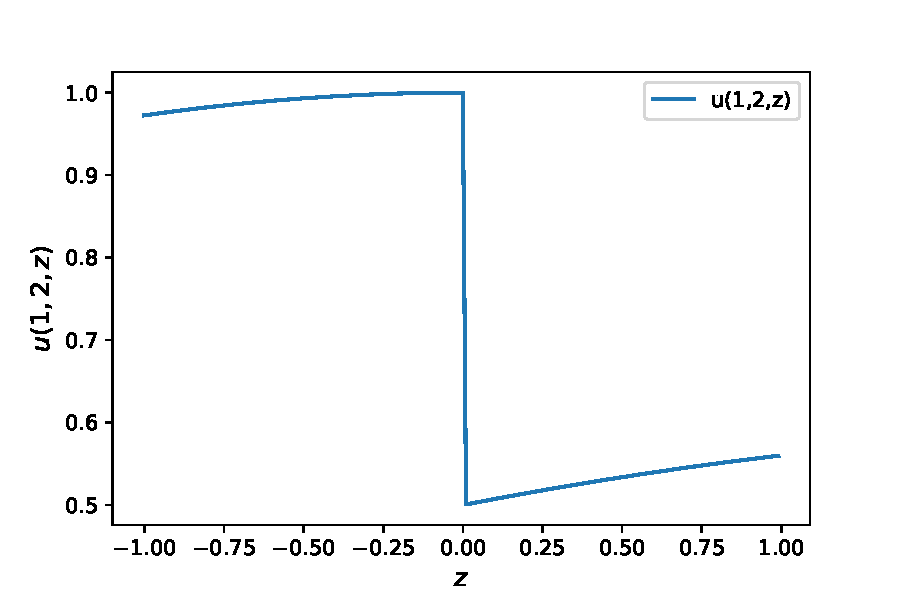
\includegraphics[width=0.8\textwidth]{gPC_hyp/c_discontinuous}
  \bicaption[2-1]{例一:显式解(\ref{ana_sol})在$t=1$和$x=2$处关于$z$间断。}{例一:显式解(\ref{ana_sol})在$t=1$和$x=2$处关于$z$间断。}{Fig}{Example 1. The analytic solution~(\ref{ana_sol}) at $t=1$ and $x=2$ is a discontinuous function of $z$.}
\end{figure}
% Figure\ref{1} shows that the analytic solution(\ref{ana_sol}) has a discontinuity at $z = 0$ when $x = 2$.  Figure\ref{2} shows that the expectation and variance of the analytic solution. In this case, one can expect a low  convergence rate of the standard gPC-SG method. 
图\ref{2-1}显示当$x = 2$时,显式解(\ref{ana_sol})在$z = 0$处有间断。图\ref{2-2}画出了显式解的期望值和方差。 在这种情况下,可以预期标准gPC-SG方法的收敛很慢。 
\begin{figure}[htbp]
  \centering
  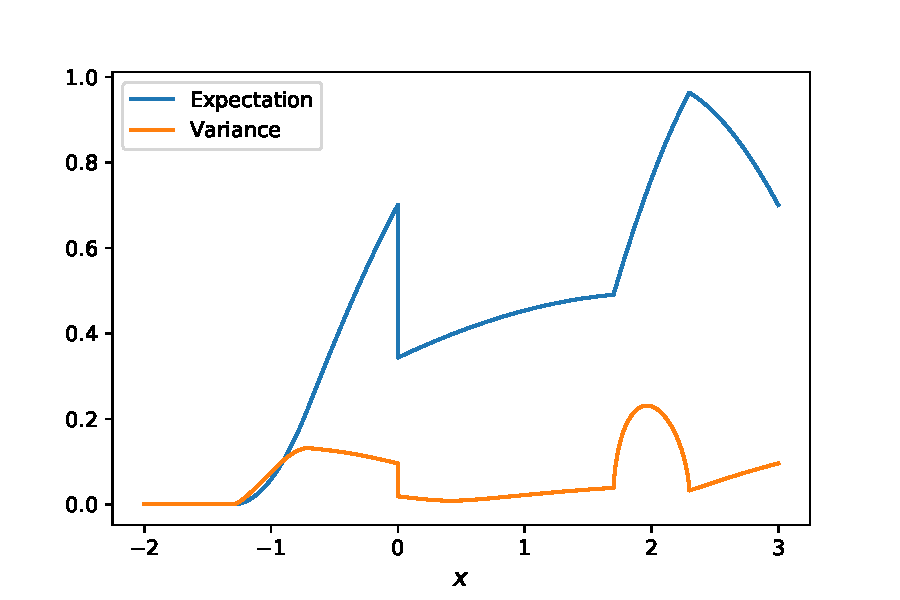
\includegraphics[width=0.8\textwidth]{gPC_hyp/c_exact}
  \bicaption[2-2]{例一:显式解的期望与方差。}{例一:显式解的期望与方差。}{Fig}{Example 1. The expectation and variance of the analytic solution.}
\end{figure}

\subsubsection{一阶差分逼近}
% In this subsection, we will give the numerical results of our discrete gPC-SG method.  Figure\ref{3} shows the numerical expectation and variance compared with the analytic solution with $\Dx = 0.001$, $\Dt = \dfrac{1}{4}\Dx$ and gPC order $K=20$. The discrepancy on the variance is due to the poor resolution of the
% first order spatial discretization, which is improved with the second order
% spatial discretization to be used later.
在本小节中,我们将给出离散gPC-SG方法的数值结果。图\ref{2-3}显示使用$\Dx = 0.001$,$\Dt = \dfrac{1}{4}\Dx$,gPC-SG阶数$K = 20$的数值解与显式解的期望与方差的比较。方差的误差是由一阶空间离散的低分辨率导致的。后面我们将使用二阶离散格式对其进行改进。

% Next we conduct the convergence test only for the gPC approximation.
% We fix $\Dx=0.005$ and $\Dt = \dfrac{1}{5}\Dx$ in all computations with
% different $K$. Figure\ref{4} shows that the $\ell^1$ error decays very fast with respect to the gPC order $K$. When $K=4$, it decays to the numerical error of the finite difference method. 
接下来,我们对gPC-SG进行收敛性测试。我们在所有计算中固定$\Dx=0.005$和$\Dt = \dfrac{1}{5}\Dx$。图\ref{2-4}显示$\ell^1$误差相对于gPC阶数$K$衰减得非常快。当$K=4$时,基本衰减到有限差分法的误差。
\begin{figure}[htbp]
  \includegraphics[width=0.5\textwidth]{gPC_hyp/c_mean}
  \includegraphics[width=0.5\textwidth]{gPC_hyp/c_var}
  \bicaption[2-3]{例一:一阶格式的数值解与显示解比较,$\Dx = 0.001$,$\Dt = \dfrac{1}{4}\Delta x$,gPC阶数$K=20$。}{例一:一阶格式的数值解与显示解比较,$\Dx = 0.001$,$\Dt = \dfrac{1}{4}\Delta x$,gPC阶数$K=20$。}{Fig}{Example 1. The analytic solution compared with the new gPC-SG method using first order finite difference approximation with $\Dx = 0.001$, $\Dt = \dfrac{1}{4}\Delta x$, gPC order $K=20$.}
\end{figure}


\begin{figure}[htbp]
  \centering
  \includegraphics[width=0.8\textwidth]{gPC_hyp/c_gpc_error}
  \bicaption[2-4]{例一:一阶离散格式$\ell^1$误差与gPC阶数的关系,$\Dx=0.005$, $\Dt=\dfrac{1}{5}\Dx$。}{例一:一阶离散格式$\ell^1$误差与gPC阶数的关系,$\Dx=0.005$, $\Dt=\dfrac{1}{5}\Dx$。}{Fig}{Example 1. The first order finite difference approximation with $\Dx=0.005$, $\Dt=\dfrac{1}{5}\Dx$: the $\ell^1$ error versus the gPC order.}
\end{figure}

% However, in Figure\ref{4}, since the finite difference error dominates the
% gPC error, it is difficult to verify the convergence rate of the gPC method. In order to examine the gPC error, we fix $\Dx$ and $\Dt$, and
% compare the numerical solutions with different $K$, with the case of $K=30$ serving as the reference solution.  We measure the $\ell^1$ error between each $K=2,3,\dotsc,20$ and $K=30$. The result is shown 
% in Figure\ref{5}, in which an exponential convergence in the gPC approximation can be observed by using the $\log$-$\log$ plot. Note that if the convergence order is algebraic, the curve should be a line.
% Here the curve shape shows the  exponential decay of the gPC error.

然而,在图\ref{2-4}中,由于有限差分的误差占主导地位(远大于gPC-SG方法的误差),这样很难验证gPC方法的收敛速度。为了验证gPC-SG的收敛性,我们固定$\Dx$和$\Dt$,用作为$K = 30$时的解作为参考解,比较$K$不同时与参考解的差别。 我们测量每个$K=2,3,\dotsc,20$和$K =30$之间的$\ell^1$误差,结果如图\ref{2-5}所示。通过对数图可以观察到gPC-SG方法是指数收敛的。

\begin{figure}[htbp]
  \centering
  \includegraphics[width=0.8\textwidth]{gPC_hyp/c_gpc_error_loglog}
  %\includegraphics[width=0.5\textwidth]{figs/c_gpc_error_logy}
  \bicaption[2-5]{例一:一阶格式的gPC-SG方法误差与gPC阶数的对数关系,$\Dx=0.005$, $\Dt=\dfrac{1}{5}\Dx$。}{例一:一阶格式的gPC-SG方法误差与gPC阶数的对数关系,$\Dx=0.005$, $\Dt=\dfrac{1}{5}\Dx$。}{Fig}{Example 1. The first order finite difference approximation $\Dx=0.005$, $\Dt=\dfrac{1}{5}\Dx$: the gPC error versus the gPC order by a log-log plot
(with other numerical parameters fixed).}
\end{figure}


%
%\begin{equation}
%  \begin{split}
%    &\text{error} \sim \mathrm{e}^{-N} \\
%    \Leftrightarrow&\log(\text{error}) \sim -N \\
%    \Leftrightarrow&\log(\text{error}) \sim -\mathrm{e}^{\log(N)}.
%  \end{split}
%\end{equation}


\subsubsection{二阶差分逼近}
% For the second order scheme, we use the same set up as in the first order case. Figure\ref{mv2} shows the expectation and variance compared with the analytic solution,
% which gives a more accurate solution than the first
% order approximation especially for the variance around $x=2$. 

% Figure\ref{mverr2} and Figure\ref{mverrlog2} show the convergence of the numerical method in the gPC order from which one can observe the fast convergence. Comparing Figure 7 with Figure 4, we can see that the second scheme has a better total $\ell^1$ error. But the rate of the gPC convergence shown in Figure\ref{mverrlog2} is  not as fast as the first order scheme. This is hardly surprising since our spectral convergence
% depends on the smoothness of the discrete solutions, and the smoothness is
% given by the numerical viscosity which is larger 
% for the first order spatial discretization. The second order spatial
% discretization offers better accuracy away from the discontinuities and better
% resolutions at discontinuities, but  because it is closer
% to the analytic solution (which is not smooth) thus less smooth than the first order one, and smoothness of the discrete solution is what 
%  our spectral convergence relies upon, thus its gPC congerence rate, compared with
% the first order one, should be slower.  However this does not mean that 
% the second order method is inferior to the first one, since one has to 
% consider the {\it overall} error, including the contributions of error from
% the spatial discretization in this problem. By comparing  Figure 6 with Figure 3, and 
% Figure 7 with Figure 4, it is obvious that the second order scheme outperforms
% the first order one.

对于二阶格式,我们用与前面一阶格式相同的设置。图\ref{mv2}画出了与显示解相比的期望值和方差,可以看到比一阶格式的结果要好,特别是方差在$x = 2$附近的近似。

图\ref{mverr2}和图\ref{mverrlog2}显示了gPC-SG方法的收敛,从中可以观察到收敛是非常之快的。比较图\ref{mverr2}和图\ref{2-4},我们可以看到二阶格式有更好的总$\ell^1$误差。但是图\ref{mverrlog2}中显示的gPC收敛的速率却不如一节格式。这点并不奇怪,因为我们的收敛速率取决于离散解的光滑性,而一阶格式给出的数值粘性较大,从而光滑性更好。二阶格式因为它更接近
于精确解(其是非常不光滑的),因此与一阶格式相比离散解的光滑性相对比较差,而这正是影响收敛速率的主要因素,所以二阶格式的收敛速度相比一阶而言较慢。然而这并不意味着二阶格式不如一阶,因为必须考虑{\it 整体的}误差,包括空间离散的误差。通过比较图\ref{mv2}与图\ref{2-3},图\ref{mverr2}与图\ref{2-4},显然二阶格式要优于一阶格式。
 
% RecaThis is due to the different treatments we use for gPC-SG method: in the f%irst order scheme we use the standard gPC-SG procedure, \ie, we can compute the% gPC projection matrix analytically, however, in the second order case we use n%umerical integration to compute the projection matrix due to the nonlinearity. %The error of numerical integration affects the convergence here which is shown %clearly between Figure 8 and Figure 5: the gPC error for the second order schem%e is larger than that for the first order scheme, \ie, when gPC $K=20$ error of% second order scheme $O(10^{-4})$ versus $O(10^{-15})$ for the first order sche%me.  
\begin{figure}[htbp]
  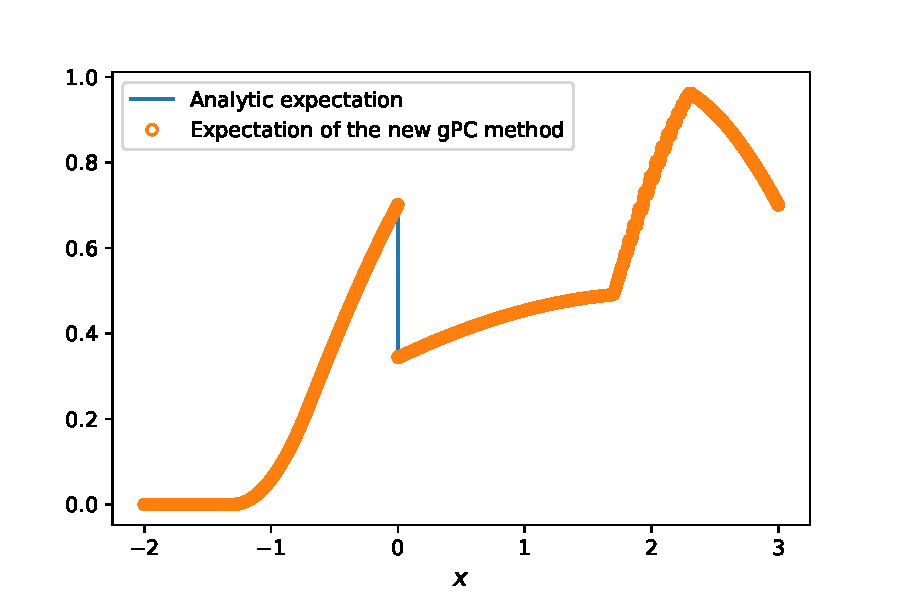
\includegraphics[width=0.5\textwidth]{gPC_hyp/mean2}
  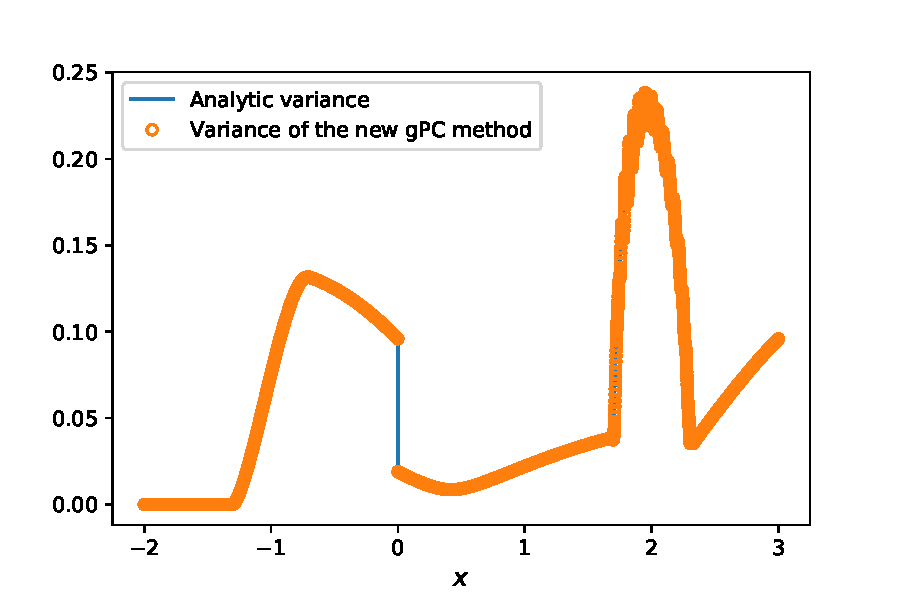
\includegraphics[width=0.5\textwidth]{gPC_hyp/var2}
  \bicaption[mv2]{例一:显式解与二阶空间离散的gPC-SG方法比较,$\Delta x = 0.001$, $\Delta t = \dfrac{1}{4}\Delta x$,gPC-SG的阶数为$K=20$。}{例一:显式解与二阶空间离散的gPC-SG方法比较,$\Delta x = 0.001$, $\Delta t = \dfrac{1}{4}\Delta x$,gPC-SG的阶数为$K=20$。}{Fig}{Example 1. The analytic solution compared with the new gPC-SG method using the second order finite difference approximation with  $\Delta x = 0.001$, $\Delta t = \dfrac{1}{4}\Delta x$, gPC order $K=20$.}
\end{figure}

\begin{figure}[htbp]
  \centering
  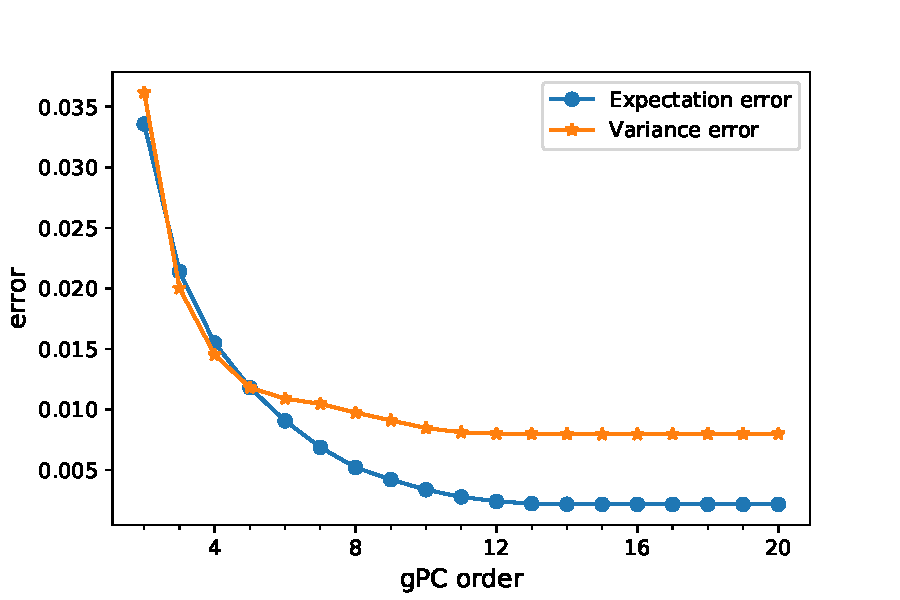
\includegraphics[width=0.8\textwidth]{gPC_hyp/gpc_err2}
  \bicaption[mverr2]{例一:二阶格式$\ell^1$误差与gPC阶数的关系,$\Dx=0.005$,$\Dt=\dfrac{1}{5}\Dx$。}{例一:二阶格式$\ell^1$误差与gPC阶数的关系,$\Dx=0.005$,$\Dt=\dfrac{1}{5}\Dx$。}{Fig}{Example 1. The second order finite difference approximation $\Dx=0.005$, $\Dt=\dfrac{1}{5}\Dx$: the 
  $\ell^1$ error versus the gPC order.}
\end{figure}

\begin{figure}[htbp]
  \centering
  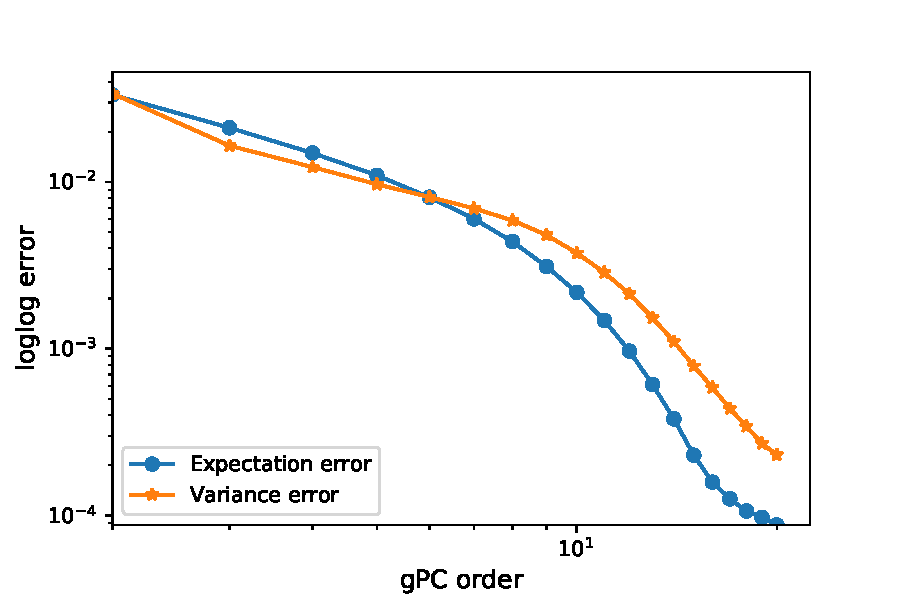
\includegraphics[width=0.8\textwidth]{gPC_hyp/gpc_err2_loglog}
  %\includegraphics[width=0.5\textwidth]{figs/gpc_err2_logy}
  \bicaption[mverrlog2]{例一:二阶格式$\ell^1$误差与gPC阶数的对数关系,$\Dx=0.005$,$\Dt=\dfrac{1}{5}\Dx$。}{例一:二阶格式$\ell^1$误差与gPC阶数的对数关系,$\Dx=0.005$,$\Dt=\dfrac{1}{5}\Dx$。}{Fig}{Example 1. The second order finite difference approximation $\Dx=0.005$, $\Dt=\dfrac{1}{5}\Dx$: the gPC error versus the gPC order by a log-log plot (with other numerical parameters fixed).}
  % \label{mverrlog2}
\end{figure}

%From numerical analysis point of view, you want to estimate the error between final numerical solution $\mathbf{U}^N_{h}$ and the exact solution $u$ on some norm, you can do this in two different ways:
%\begin{equation} \label{error1}
%||\mathbf{U}^N_{h}-u||\leq||\mathbf{U}^N_{h}-\mathbf{U}^N||+||\mathbf{U}^N-u||
%\end{equation}
%or
%\begin{equation} \label{error2}
% ||\mathbf{U}^N_{h}-u||\leq||\mathbf{U}^N_{h}-U_h||+||U_h-u||.
%\end{equation}
%And for our problem if you do as (\ref{error1}), the $||\mathbf{U}^N-u||$ part can not be estimated. If you do in the second way (\ref{error2}), $|U_h-u||$ can be obtained as the same in Qi Peng's paper (that depends on $z$), $||\mathbf{U}^N_{h}-U_h||$ can be obtained in the standard gPC way. 

\subsection{例二:带有随机间断势的刘维尔方程}

再次写出刘维尔方程
\begin{equation}
  u_t+v u_x-V_x u_v=0, \quad t>0, \quad x,v\in R,
\end{equation}
其中随机势如下
\begin{equation}
  V(x,y)=V_0(x)+0.1xz,
\end{equation}
$z$为$(-1,1)$上的均匀分布,
\begin{equation}
  V_0(x)=
  \begin{cases}
    0.2, \quad &x<0, \\
    0, \quad &x>0.
  \end{cases}
\end{equation}

% For the given initial data, one cannot get an analytic solution for this problem. Instead we will use the {\it collocation method} as a comparison. In collocation method, one solves the Liouville equation(\ref{eq_Liou}) at a discrete set of $\{z_i\}_{1\leq i\leq M}$ called sample points in the corresponding random space. For every fixed $z_i$, we only need to solve a {\it deterministic} Liouville equation with discontinuous potential using Hamilton preserving scheme\citen{Wen:2005ueba}. Then the expectation and variance can be obtained by the quadrature rules of(\ref{exp}) and(\ref{var}). In the following examples, we choose $\{z_i\}_{1\leq i\leq M}$ as the roots of $M$th order Legendre polynomials and use the Gauss-Legendre quadrature to obtain the expectation and variance.

对于给定的初始数据,因为无法得到这个问题的显式精确解。所以,我们将使用{\it 配点法}(stochastic collocation method)作为参考解。在配点法中,在对应的随机空间中取$\{z_i\}_{1\leq i\leq M}$的离散点集合,称为抽样点,我们在只需在抽样点上解刘维尔方程(\ref{eq_Liou})。 对于每个固定的$z_i$,我们只需要使用用来解{\it 确定性} 的带间断势的刘维尔方程的哈密顿守恒格式。然后,可以通过(\ref{exp})和(\ref{var})通过数值积分获得期望和方差。在以下示例中,我们选择$\{z_i\}_{1\leq i\leq M}$作为$M$阶勒让德多项式的根,并使用高斯积分来获得期望值和方差。

% For the gPC method we need to evaluate $\int_{-1}^1 V_0(z)P_j(z)P_k(z) \rho(z)\diff z$, which, for this simple case, is given by
对于gPC-SG方法我们需要计算$\int_{-1}^1 V_0(z)P_j(z)P_k(z) \rho(z)\diff z$也就是,
\begin{equation}
  \int_{-1}^1 V_0(z)P_j(z)P_k(z) \rho(z)\diff z =
  \begin{cases}
    \dfrac{j+1}{\sqrt{(2j+1)(2j+3)}}, &k=j+1, \\
    V'_0(x), &k=j, \\
    \dfrac{j}{\sqrt{4j^2-1}}, &k=j-1.
  \end{cases}
\end{equation}
这里我们得到一个对称的三对角矩阵。

% As an illustration of the singularity of the solution caused by the discontinuous potential , we use a continuous initial data:
为了说明由间断的势导致的解的奇异性,我们使用连续的初值:
\begin{equation}
  u(x,v,0)=
  \begin{cases}
  \sin[2\pi(0.25-(x^2+v^2))], &x^2+v^2<0.25, \\
  0, &\text{其他}.
  \end{cases}
\label{ex2-init2}
\end{equation}
% The expectation of the solution by using the collocation method with $M=20$ sample points and our new gPC-SG method with gPC order $K=4$ are shown in Figure\ref{2-8}. 
由配点法($M=20$个抽样点)和我们的$K=4$阶离散gPC-SG方法期望与方差如下图\ref{2-8}所示。
\begin{figure}[htbp]
  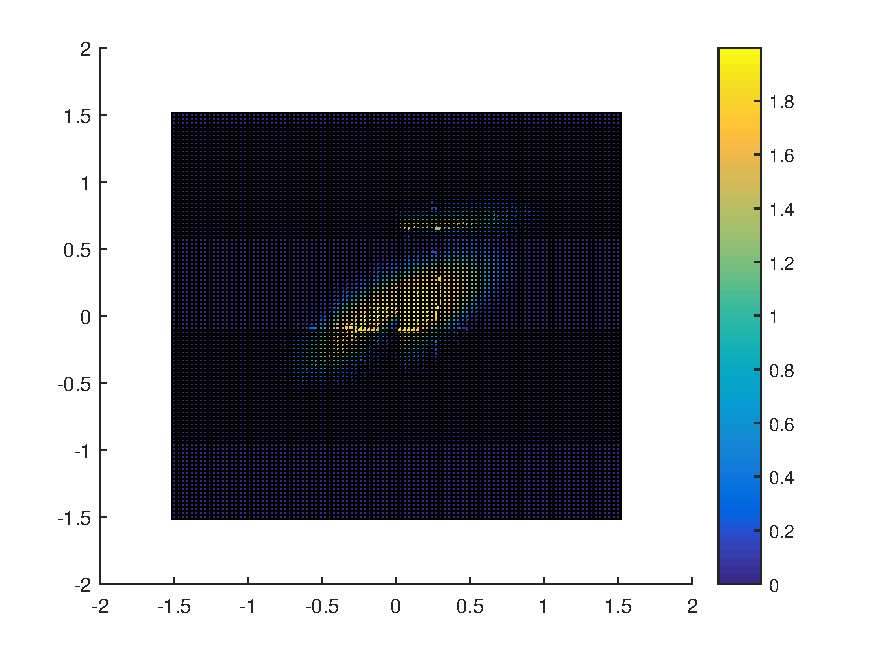
\includegraphics[width=0.5\textwidth]{gPC_hyp/pseudoSpecSmooth}
  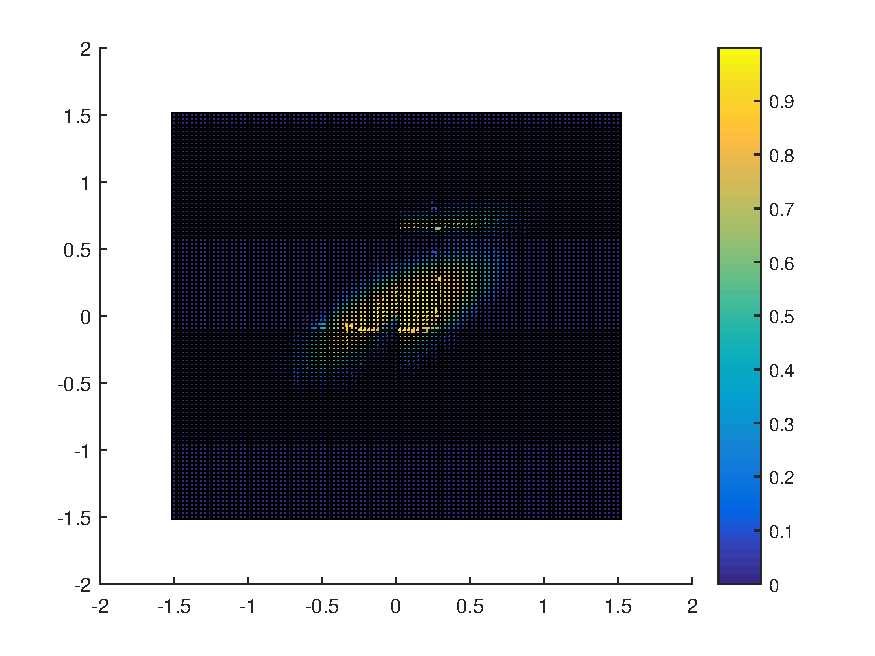
\includegraphics[width=0.5\textwidth]{gPC_hyp/galerkinsmooth}
  \bicaption[2-8]{例二:初值为(\ref{ex2-init2})。由配点法(左)与离散gPC-SG方法(右)得到的期望。}{例二:初值为(\ref{ex2-init2})。由配点法(左)与离散gPC-SG方法(右)得到的期望。}{Fig}{Example 2 with initial data (\ref{ex2-init2}). Expectation of the solution. Left: the collocation method with $20$ sample points. Right: the new gPC-SG method with gPC order $K=4$.}
  % \label{2-8}
\end{figure}
% Although the initial data is continuous, due to the interface condition, the solution may still be discontinuous. This singularity will have a big impact on the convergence of gPC method.
虽然初值是连续的,但由于界面条件的存在,解仍然是间断的。而这种奇异性会大大影响gPC-SG方法的收敛性。

\subsubsection{一阶差分逼近}
在这个例子里,我们考虑初值
\begin{equation}
  u(x,v,0)=
  \begin{cases}
    1, \quad &x\geq 0, v<0, x^2+v^2<1, \\
    1, \quad &x\leq 0, v>0, x^2+v^2<1, \\
    0, \quad &\text{其他}.
  \end{cases}
\label{ex2-init1}
\end{equation}
% Notice that the solution has singularity due to both the initial data and the discontinuous potential. The deterministic version of this example was used in\citen{Wen:2005ueba} and the analytic solution can be obtained by using the method of characteristics. We first plot the analytic solution and numerical solution (using the first order flux) with a fixed $z=0$ in Figure\ref{2-9} corresponding to the deterministic example in\citen{Wen:2005ueba}.

注意,由于初始数据和势的不连续性从而导致解具有奇异性。该示例的确定性版本在\citen{Wen:2005ueba}中被使用过,并且可以通过使用特征线的方法获得显式精确解。 我们首先在画出对应于\citen{Wen:2005ueba}中的确定性示例的图\ref{2-9},包括显示精确解和数值解(使用一阶通量),其中固定$z = 0$。
\begin{figure}
  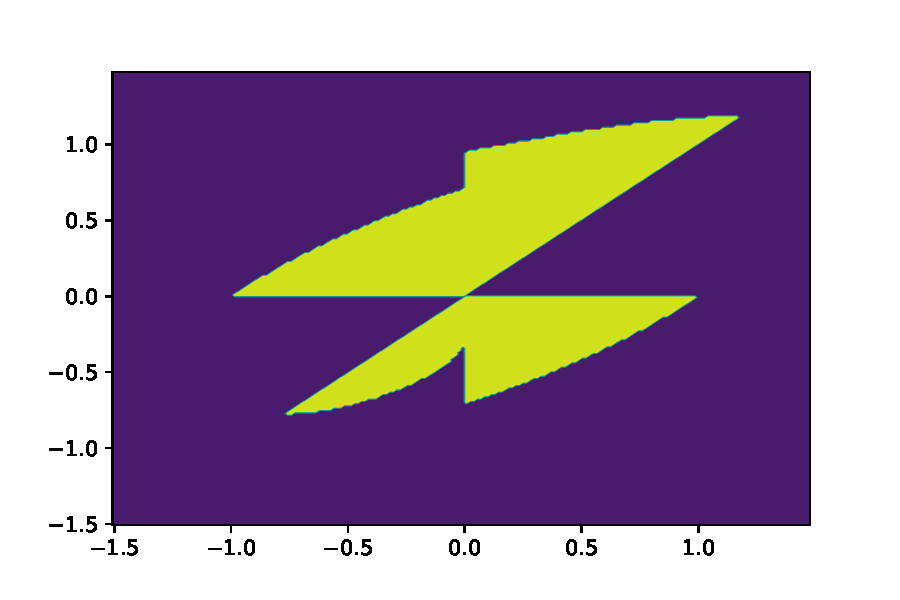
\includegraphics[width=0.5\textwidth]{gPC_hyp/exact}
  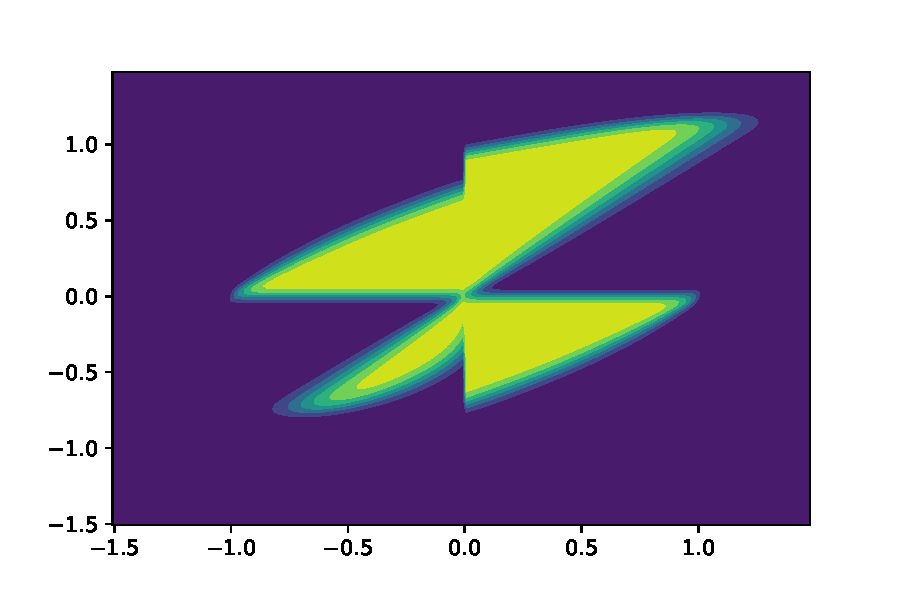
\includegraphics[width=0.5\textwidth]{gPC_hyp/num_1}
  \bicaption[2-9]{例二的确定性版本,初值(\ref{ex2-init1})。显式精确解(左),数值解(右),$\Delta x = \Delta v = 0.015$,$\Delta t = 0.001$。}{例二的确定性版本,初值(\ref{ex2-init1})。显式精确解(左),数值解(右),$\Delta x = \Delta v = 0.015$,$\Delta t = 0.001$。}{Fig}{The deterministic case of Example 2 with initial data (\ref{ex2-init1}). Left: analytic solution of the deterministic problem with $z=0$ and $t=1$. Right: numerical solution using the first order Hamiltonian preserving scheme with $\Delta x = \Delta v = 0.015$, $\Delta t = 0.001$.}
  % \label{2-9}
\end{figure}

% Then we compare the solution computed by the collocation method with $M=20$ sample points (Figures\ref{2-6} and\ref{2-15} left). Figures\ref{2-6} and\ref{2-15} right show the solutions  by our new gPC-SG method with gPC order $K=10$. Here the mesh size is $\Dx=\Dv=0.03$ and time step is $\Dt=0.002$. One can see the difference between the expectation of the stochastic solution and the deterministic case when $z=0$ and this differences can be easily seen on the variance plots as well. The expectation of the stochastic solution is expected to be smoother
% since it integrates over the $z$ variable, thus gains on order of regularity
% (see examples in \citen{Des, HJX}).
% For the computation cost, our new gPC-SG method runs much faster than collocation method. The collocation method takes about $20$ times cost of the deterministic version due to $20$ sample points we choose, however, our new gPC-SG,
% with $K=10$,  takes about $10$ times the cost of the deterministic problem.

然后我们与用配点法计算的解($M = 20$样本点)(图\ref{2-6}和\ref{2-15}左)进行比较。图\ref{2-6}和\ref{2-15}右显示我们的新gPC-SG方法的解,其中gPC阶数$K = 10$。这里的网格大小是$\Dx = \Dv = 0.03$,时间步长是$\Dt = 0.002$。可以看到随机方程的解的期望和当$z = 0$的确定性情况之间的差异,并且这种差异也可以容易地在方差图上看出。随机方程的解的期望更加光滑,因为它对$z$变量进行了积分(相当于平均),从而得到了更好的正则性(参见\citen{Des, HJX})。关于计算的开销,我们的新的离散gPC-SG方法运行比配点法要快得多。 配点法要花费大约$20$倍确定性版本的成本,因为我们使用了$20$个样本点;然而,我们的新的离散gPC-SG,阶数$K = 10$(即可得到优于配点法$20$个样本点的解),花费大约$10$倍确定性问题的成本。

\begin{figure}[htbp]
% \centering
  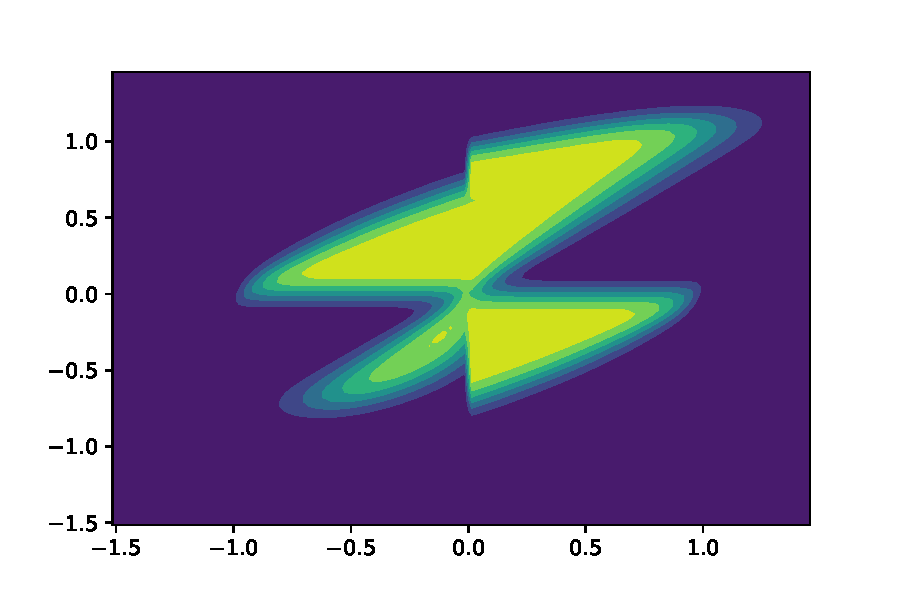
\includegraphics[width=0.5\textwidth]{gPC_hyp/col_mean_1}
  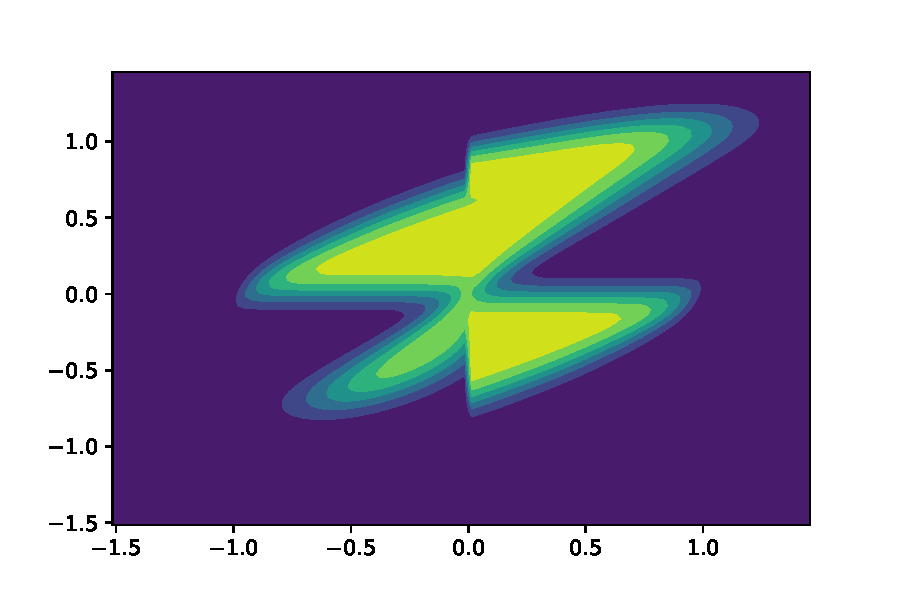
\includegraphics[width=0.5\textwidth]{gPC_hyp/mean_1}
  \bicaption[2-6]{例二:初值为(\ref{ex2-init1}),由一阶差分格式得到的期望,配点法(左)与离散gPC-SG方法(右),$\Dx=\Dv=0.03$,$\Dt=0.002$。}{例二:初值为(\ref{ex2-init1}),由一阶差分格式得到的期望,配点法(左)与离散gPC-SG方法(右),$\Dx=\Dv=0.03$,$\Dt=0.002$。}{Fig}{Example 2 with initial data (\ref{ex2-init1})  by the first order 
finite difference approximation  with $\Dx=\Dv=0.03$ and $\Dt=0.002$.  The expectation of the solution. Left: the collocation method with $M=20$ samples points. Right: the new gPC-SG method using first order finite difference approximation.}
  % \label{2-6}
\end{figure}
\begin{figure}[htbp]
% \centering
  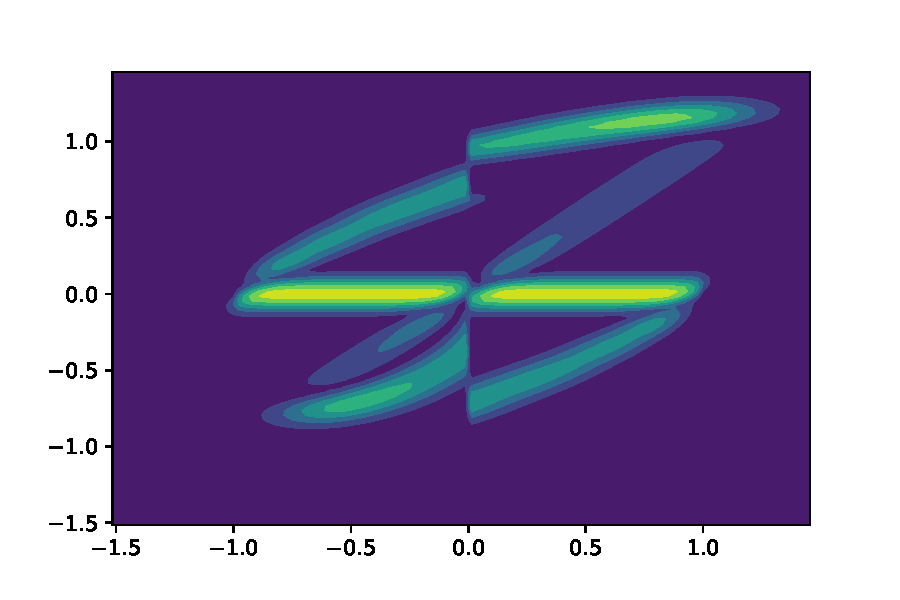
\includegraphics[width=0.5\textwidth]{gPC_hyp/col_var_1}
  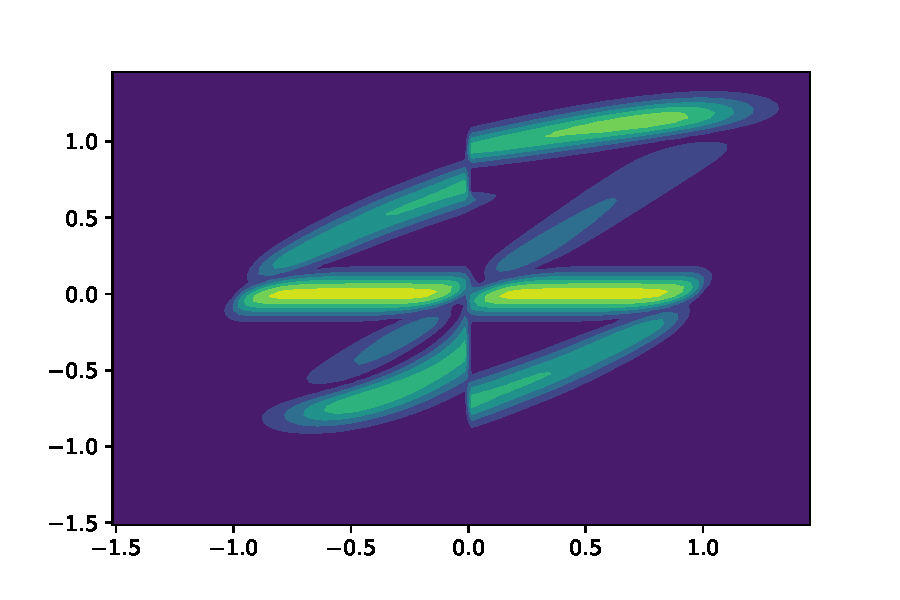
\includegraphics[width=0.5\textwidth]{gPC_hyp/var_1}
  \bicaption[2-15]{例二:初值为(\ref{ex2-init1}),由一阶差分格式得到的方差,配点法(左)与离散gPC-SG方法(右),$\Dx=\Dv=0.03$,$\Dt=0.002$。}{例二:初值为(\ref{ex2-init1}),由一阶差分格式得到的方差,配点法(左)与离散gPC-SG方法(右),$\Dx=\Dv=0.03$,$\Dt=0.002$。}{Fig}{Example 2 with initial data (\ref{ex2-init1}) by the first order 
finite difference approximation  with $\Dx=\Dv=0.03$ and $\Dt=0.002$. The variance of the solution. Left: the collocation method. Right: the new gPC-SG 
method.}
  % \label{2-15}
\end{figure} 

% In Figure\ref{2-7} we plot the $\ell^1$ error of the discrete gPC-SG method as the gPC order $K$ increases. This figure shows the spectral convergence.
在图\ref{2-7},我们画出离散gPC-SG方法的$\ell^1$误差随着gPC阶数$K$增加的变化关系,显示出了谱收敛结果。
\begin{figure}[htbp]
  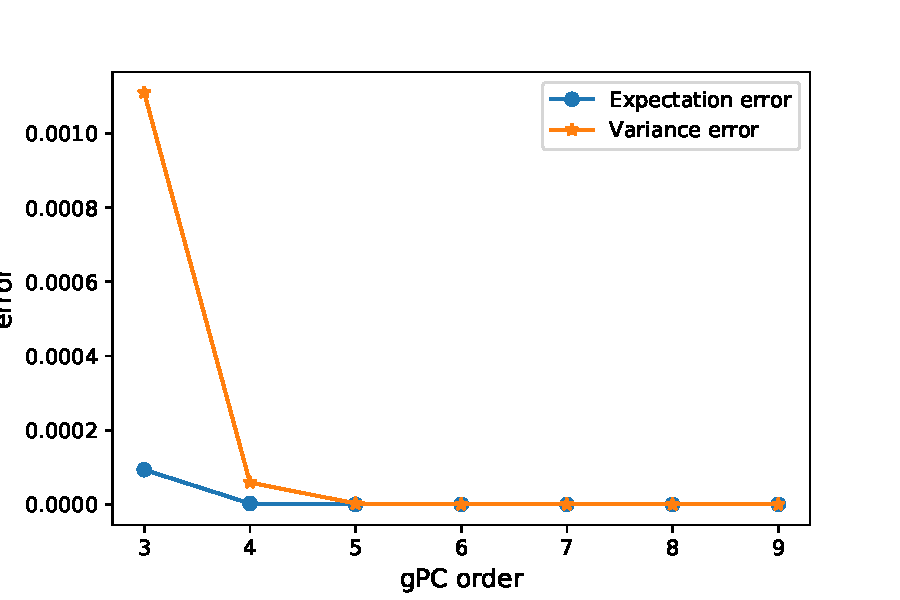
\includegraphics[width=0.5\textwidth]{gPC_hyp/convergence_1}
  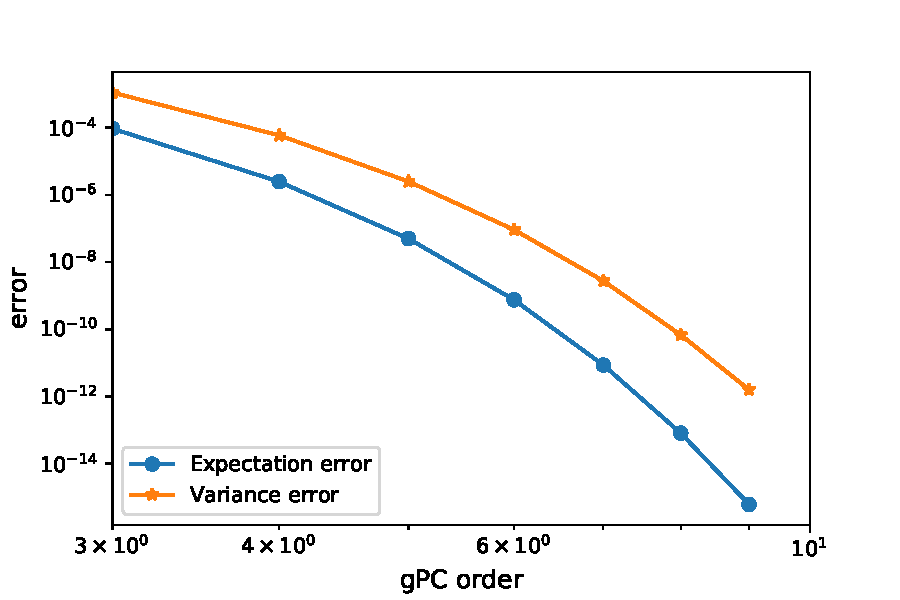
\includegraphics[width=0.5\textwidth]{gPC_hyp/loglog_conv_1}
  \bicaption[2-7]{例二:初值(\ref{ex2-init1}),一阶离散gPC-SG方法的$\ell^1$误差随着gPC阶数$K$增加的变化关系(左)及对数图(右)。}{例二:初值(\ref{ex2-init1}),一阶离散gPC-SG方法的$\ell^1$误差随着gPC阶数$K$增加的变化关系(左)及对数图(右)。}{Fig}{Example 2 with initial data (\ref{ex2-init1}). Convergence of the new gPC-SG method using the first order finite difference approximation. Left: the $\ell^1$ error versus gPC order. Right: the gPC error versus the gPC order by a log-log plot (with other numerical parameters fixed).}
  % \label{2-7}
\end{figure}






\subsubsection{二阶差分格式}
% Here for the second finite difference approximation we still use the same set up as in previous subsection for the first order case. 
这里对于二阶差分格式,我们使用和前面一阶格式类似的参数设定。
% We also calculate the $\ell^1$ error between our numerical method ({\bf Jin remark: is this for deterministic or random potential?  If deterministic, what do you mean ``our method'' and why you need this which was already known previously?}) and the reference solution, and the results are given in Table\ref{10}.
% \begin{table}
% \centering
%   \begin{tabular}{ c|c|c|c| }
%   $\Delta x$ & 0.06 & 0.03 & 0.015 \\ \hline
%   $\ell^1$ error & 0.288 & 0.165 & 0.094 \\
% \end{tabular}
%   \caption{$\ell^1$ error and meshsize}
%   \label{10}
% \end{table}
% We can see that although we use a second order flux, the whole scheme's convergence rate cannot be more than half, as was previously proven
% in \citen{Wen:2005ueba,Qi:2013byba}.

% First as in the first order case, we will show the numerical solution of the deterministic case when $z=0$ using the second order flux in Figure\ref{deter_sec}.  The second order method clearly gives a much sharper resolution for the discontinuities than the first order method (compare the right figures of
% Figure 10 and Figure 15). But due to the Lax-Wendroff scheme we use in the $v$-direction(\ref{vflux}), there exists some oscillations due to numerical dispersion.
首先,如同一阶的情形,我们在\ref{deter_sec}中画出由二阶格式得到的$z=0$时确定性的方程的数值解。二阶格式明显给出了高分辨率的结果(相比一阶格式,见图\ref{2-9}和图\ref{2-11})。但是由于在$v$方向我们用的是Lax-Wendroff格式,所以这里有一些数值振荡。
\begin{figure}{}
  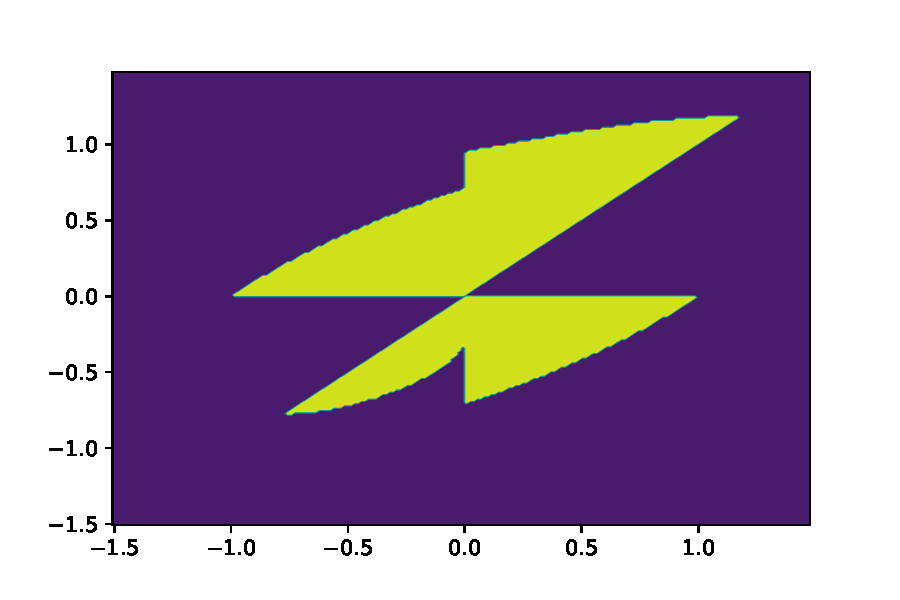
\includegraphics[width=0.5\textwidth]{gPC_hyp/exact}
  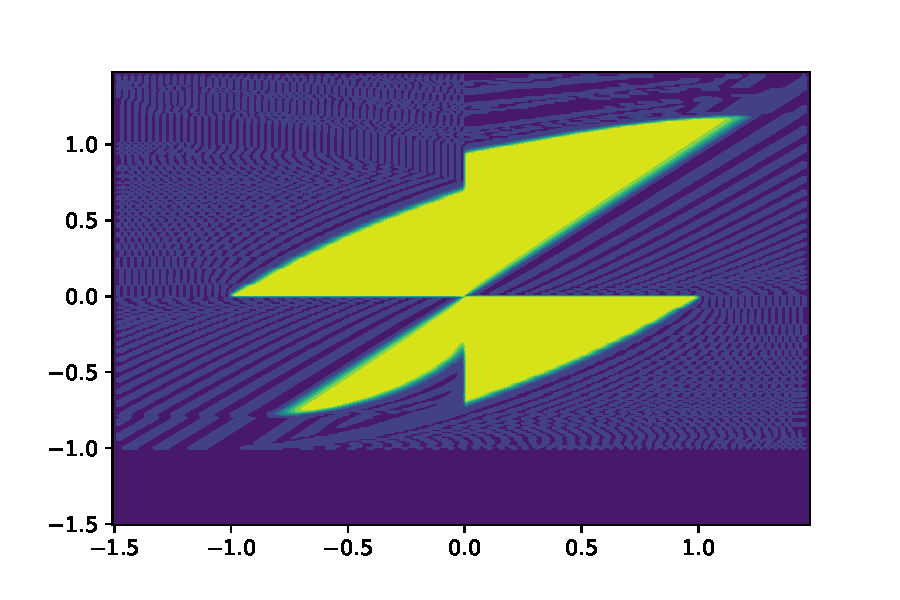
\includegraphics[width=0.5\textwidth]{gPC_hyp/num}
  \bicaption[deter_sec]{例二:初值为(\ref{ex2-init1})的确定性版本。左图为显式精确解($z=0$,$t=1$);右图为二阶格式的数值解,$\Delta x = \Delta v = 0.015$,$\Delta t = 0.001$。}{例二:初值为(\ref{ex2-init1})的确定性版本。左图为显式精确解($z=0$,$t=1$);右图为二阶格式的数值解,$\Delta x = \Delta v = 0.015$,$\Delta t = 0.001$。}{Fig}{The deterministic case of Example 2 with initial data~(\ref{ex2-init1}). Left: analytic solution of the deterministic problem with $z=0$ and $t=1$. Right: numerical solution using the second order Hamiltonian preserving scheme with $\Delta x = \Delta v = 0.015$, $\Delta t = 0.001$}
  % \label{deter_sec}
\end{figure}

% Then we will show the expectation and variance of the solution calculated by the collocation method with $M=20$ sample points and our new gPC-SG method (for the calculation of $\left<\mathrm{RHS}(z)\right>$ we also use 20 Gauss-Legendre quadrature points). See Figure\ref{2-11} and Figure\ref{2-12}.
接下来我们对比由配点法和离散gPC-SG方法计算的期望与方差,见图\ref{2-11}和\ref{2-12}:
\begin{figure}
  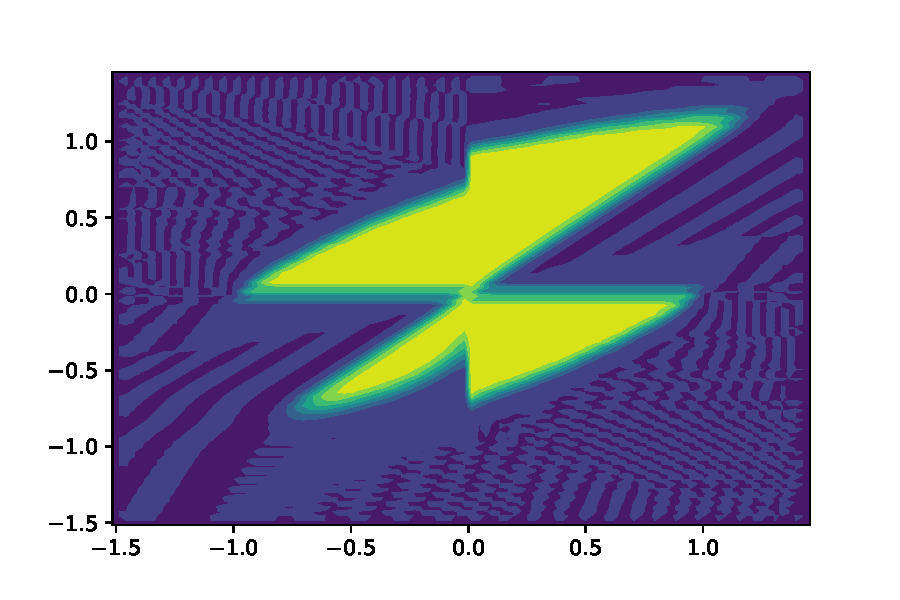
\includegraphics[width=0.5\textwidth]{gPC_hyp/col_mean}
  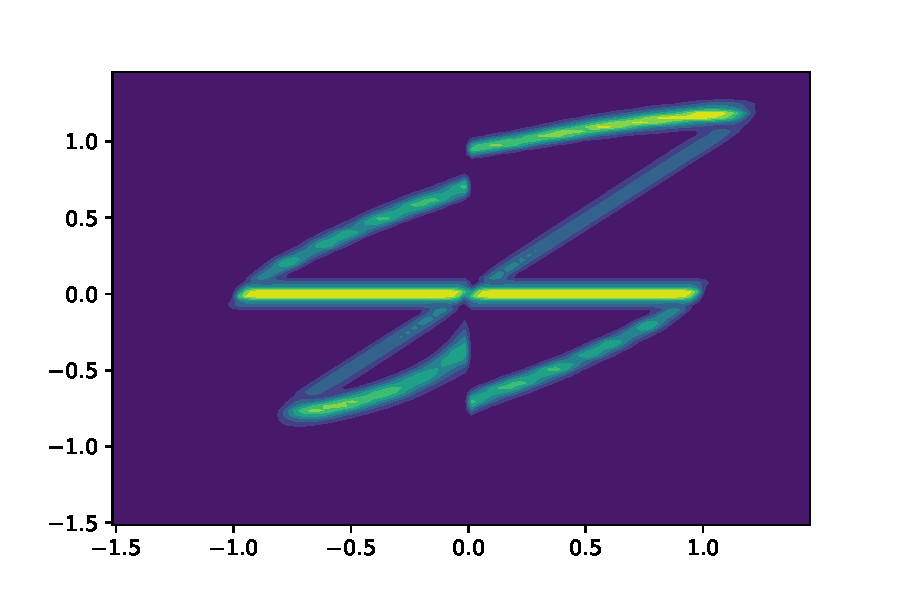
\includegraphics[width=0.5\textwidth]{gPC_hyp/col_var}
  \bicaption[2-11]{例二:初值为\ref{ex2-init1}),二阶离散配点法的解,期望(左)和方差(右),$\Delta x = \Delta v = 0.03$,$\Delta t = 0.002$。}{例二:初值为\ref{ex2-init1}),二阶离散配点法的解,期望(左)和方差(右),$\Delta x = \Delta v = 0.03$,$\Delta t = 0.002$。}{Fig}{Example 2 with initial data (\ref{ex2-init1}) by the second order 
finite difference approximation  with $\Delta x = \Delta v = 0.03$, $\Delta t = 0.002$. Reference solution 
 by the collocation method with 20 sample points at $t=1$. Left: expectation. Right: variance.}
  % \label{2-11}
\end{figure}
\begin{figure}
  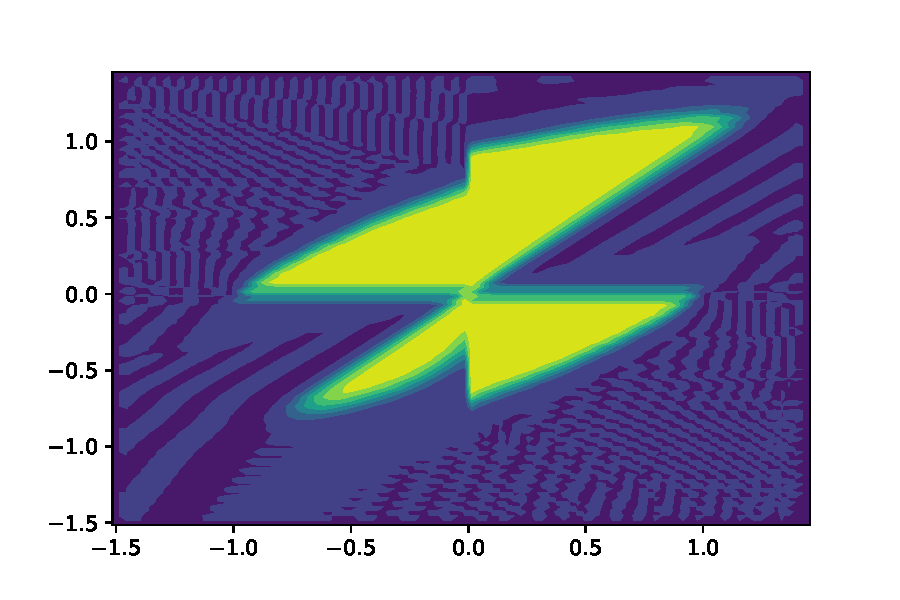
\includegraphics[width=0.5\textwidth]{gPC_hyp/mean}
  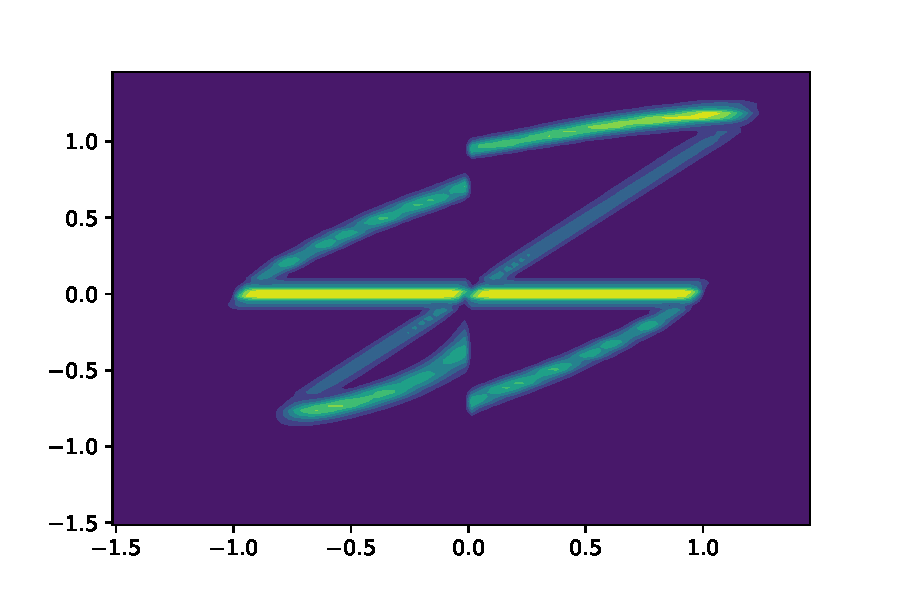
\includegraphics[width=0.5\textwidth]{gPC_hyp/var}
  \bicaption[2-12]{例二:初值为\ref{ex2-init1}),二阶离散gPC-SG的结果,期望(左)和方差(右),$\Delta x = \Delta v = 0.03$,$\Delta t = 0.002$。}{例二:初值为\ref{ex2-init1}),二阶离散gPC-SG的结果,期望(左)和方差(右),$\Delta x = \Delta v = 0.03$,$\Delta t = 0.002$。}{Fig}{Example 2 with initial data (\ref{ex2-init1}) by the second order 
finite difference approximation  with $\Delta x = \Delta v = 0.03$, $\Delta t = 0.002$. Solution at $t=1$ computed by the new gPC-SG method. Left: expectation. Right: variance.}
  % \label{2-12}
\end{figure}
% One can find no difference between these two methods, both giving sharper
% resolutions at discontinuities than their first order counterparts shown in
% Figures 11 and 12. Here for the computation cost, we point out that unlike in the first order case, our new gPC-SG method runs only slightly faster than the collocation method since in the calculation of $\left<\mathrm{RHS}(z)\right>$ we use a similarly technique as the collocation method.
可以看到二者的结果没有显著差异,在街的间断处都给出了比一阶格式更好的结果。这里对于计算的花费,我们的离散gPC-SG方法比配电法要稍快一些,因为在计算$\left<\mathrm{RHS}(z)\right>$时我们用了和配点法类似的思想。

% Finally, we test the convergence rate of our new gPC-SG method. To do this, we first fix our mesh size: $\Delta x = \Delta v = 0.03$, $\Delta t = 0.02$, and output the result at $t=1$. We  use $20$ Gauss-Legendre quadrature points to compute the inner product in (\ref{gPC2}). We choose the gPC order $K=10$ as our reference solution, and see how the error changes when increasing $K$ from $3$ to $10$. From Figure\ref{2-14}, an exponential convergence can be observed.
最后,我们来测试离散gPC-SG方法的收敛速率。首先固定网格参数:$\Delta x = \Delta v = 0.03$,$\Delta t = 0.02$,$t=1$。用$20$个点的高斯积分来计算内积(\ref{gPC2})并选择gPC阶数$K=10$为参考解来看$K$从$3$增加到$10$时误差的变化。从图\ref{2-14}可以看出谱收敛的结果。
% \begin{figure}
%   \centering
%   \includegraphics[width=0.8\textwidth]{figs/convergence}
%   \caption{The relationship between he gPC order and $l^1$ error. Green: the error of variance. Blue: the error of mean value.}
%   \label{13}
% \end{figure}
\begin{figure}
%  \includegraphics[width=0.5\textwidth]{figs/semilog_conv}
  \includegraphics[width=0.5\textwidth]{gPC_hyp/convergence}
  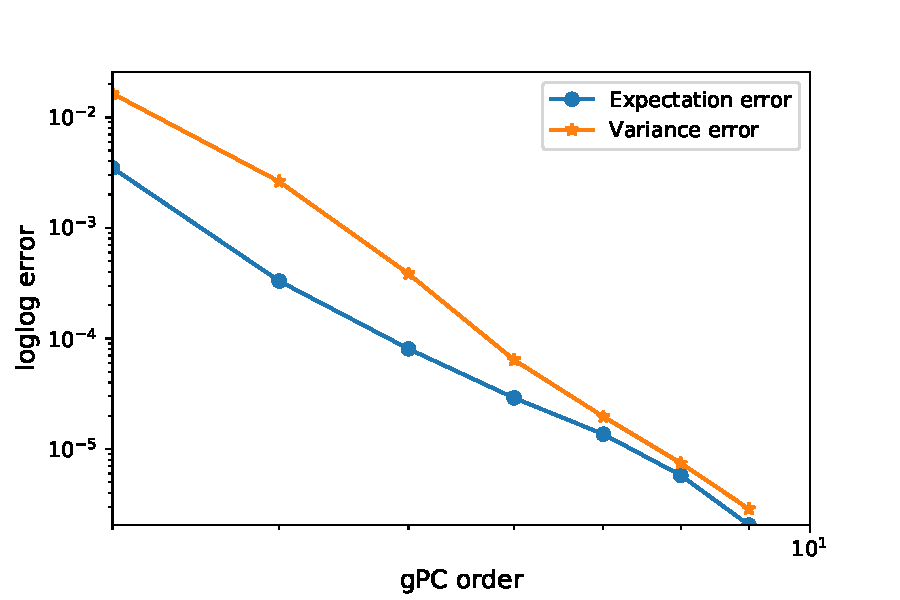
\includegraphics[width=0.5\textwidth]{gPC_hyp/loglog_conv}
  \bicaption[2-14]{例二:初值(\ref{ex2-init1}),二阶离散gPC-SG方法的收敛性,$\ell^1$误差与gPC阶数的关系图(左)和相应的对数图(右)。}{例二:初值(\ref{ex2-init1}),二阶离散gPC-SG方法的收敛性,$\ell^1$误差与gPC阶数的关系图(左)和相应的对数图(右)。}{Fig}{Example 2 with initial data (\ref{ex2-init1}). Convergence of the new gPC-SG method using second order finite difference approximation. Left: the $\ell^1$ error versus the gPC order. Right: the gPC error versus the gPC order by a log-log plot (with other numerical parameters fixed).}
  % \label{2-14}
\end{figure}

\section{本章总结与展望}
在本章中,我们研究了带有间断与随机系数的双曲型方程的数值解法。为了克服由解的奇异性导致的gPC-SG方法收敛速度很慢的问题,我们提出了离散gPC-SG方法,利用离散的解具有较好的正则性,进而改进gPC-SG方法的收敛速度。对于对流方程我们进行了收敛性分析与误差估计。同时为了说明方法的有效性,我们对于对流方程与刘维尔方程进行了大量的数值实验。

对于不光滑的、带有不确定性的问题,gPC-SG方法的应用仍然有很多问题没有解决。上述离散gPC-SG方法在高阶格式构造、非线性问题上仍然存在一定困难,同时如何将该方法向更广泛的问题上进行推广仍然需要大量的研究,会作为未来的研究方向之一。

% \begin{remark}
%   For this second order Liouville equation using our gPC scheme, there still exists many challenges in programming where we need to reduce the CPU time technically. The most time consuming part of this program is the ``FOR'' statements and the condition statements in each ``FOR'' loop (which are very slow in languages such as Python and Matlab). So for our numerical examples, we use $3$ tricks to reduce the computation cost:
%   \begin{itemize}
%     \item Most of the reduced cost is due to the special example we use: the discontinuity of potential only happens at one or few points. So for example we have 100 points in $x$ direction and 100 points in $v$-direction, in general case we should run a $100 \times 100$ loop, however, since the Hamilton preserving condition only takes effect at the two points near by the discontinuity point, we only need to run a $2 \times 100$ loop instead of a full $100 \times 100$ loop. All the left points we don’t need to run any ``FOR'' loop, we just use a vectorized formula (standard second order scheme) to iterate and then modified some of the value using the $2 \times 100$ loop.
%     \item Another part is the condition statements ``if'' in every loop, this is also a huge part of total complexity. We need to determine if $v>0$ or $v<0$ and also $v^2 + 2(V^- - V^+) > 0$ such conditions. The trick here is that we don't want to do the ``if'' judgment, instead because we iterate $v$ in an ascending order, we can know at which step $v$ changes sign (\ie just after the 50th step). So using this trick we can make most of judge statements disappear.
%     \item Some of the index change can be pre-computed. For example, for the reflection part, we can compute it before the whole iteration. But for the transmission part, because it needs a linear interpolation we don’t make it pre-computed so far.
%   \end{itemize}
%   By using these tricks, we can reduce the CPU time by 30 times.
% \end{remark}

%\section{Conclusion}
%In this work, we discuss some new results on the convection equation with disc%ontinuous and random wave speed and the Liouville equation with discontinuous %potentials. The numerical results of our new discrete gPC scheme are shown.


% \subsubsection{The numerical results of the standard gPC scheme}
% In this part, to make a comparison, I will provide the results of a ``standard'' gPC method. All the figures has a one to one corresponding with the figures in above section.

% \begin{figure}[htbp]
%   \includegraphics[width=0.5\textwidth]{c_mean}
%   \includegraphics[width=0.5\textwidth]{c_var}
%   \caption{The standard gPC scheme compared with exact solution: $\Delta x = 0.001$, $\Delta t = 0.25\Delta x$, gPC order $N=30$}
% \end{figure}
% Figure 7 is the validation of the method, which we see a little bit sharper at $x=0$ than the relaxation-gPC method. This is due to the relaxation system is a approximation to the original equation. 
% \begin{figure}[htbp]
%   \centering
%   \includegraphics[width=0.8\textwidth]{c_gpc_error}
%   \caption{The $l^1$ error respect to gPC order.}
% \end{figure}

% Figure 8 also shows the error decay respect to gPC order. In the standard gPC method, the error is smaller than the relaxation one. (The same reason as Figure 7.)

% \begin{figure}[htbp]
%   \includegraphics[width=0.5\textwidth]{c_gpc_error_loglog}
%   \includegraphics[width=0.5\textwidth]{c_gpc_error_logy}
%   \caption{The standard gPC scheme error compared with reference solution. Left: a loglog error. Right: a semilog error.}
% \end{figure}

% Next we choose gPC order $N=30$ as reference solution to test the convergence rate. In Figure 9 shows the results, comparing with the relaxation method, the standard gPC method also shows a exponential convergence which is really surprising me. Although the error is a little larger (See Figure 6 for comparison), this seems a contradiction with the convergence theory. For this issue, I will have a fully discussion in the next section.

% \subsection{Standard gPC method with wavelets as basis}
% In this part, to see the strategy of changing basis, I only give one figure to show the convergence rate to compare with Figure 6, Figure 9. In this test we use the Haar wavelets as basis, and all the other configuration is the same as the standard gPC approach. The results are shown in Figure 10

% \begin{figure}[htbp]
%   \includegraphics[width=0.5\textwidth]{c_wavelet_error_loglog}
%   \includegraphics[width=0.5\textwidth]{c_wavelet_error_logy}
%   \caption{The standard gPC scheme using wavelets as basis: $l^1$ error compared with reference solution. Left: a loglog error. Right: a semilog error.}
% \end{figure}

% We can see the results are really bad, the convergence is very slow compared with previous methods.


% \section{Discussion and analysis of the numerical results}
% In this section, I will go further to discuss the issues I find in the numerical tests and the understanding of this problem.

% At first, from the tests, we can verify that the relaxation-gPC method achieves an exponential convergence, this is not surprising as I have mentioned through all this report. Also, the error of this method (compared to the analytic solution) is a little bit larger than the standard gPC method which is, also not surprising, because the relaxation system is only a approximation of the original equation. Only when $\varepsilon$ is very small, this error should be very small.

% At a second glance at the results, a question comes out: why the ``standard" gPC method also seems to achieve the same exponential converge? It seems unusual and quite surprising. Firstly, let me say, the program is absolutely right. Secondly, the analytic solution indeed has singular which means very very bad regularity in random space as shown in Figure 2. So what's wrong? If so, does it mean the relaxation scheme is useless? To answer these questions, I will give a carefully analysis of these schemes. 

% \subsection{Explaination of the results by ``Standard" gPC Galerkin scheme}
% To make things clear, I first try to following the standard procedure and write down the whole scheme. The notations here is basically the same as in Section 2.2.

% In gPC Galerkin method, we seek an approximate solution in the form of gPC expansion, i.e.
% \begin{equation}\label{expansion}
%   u(t,x,z) = \sum_{k=0}^N\hat{u}_k(t,x)P_k(z)
% \end{equation}
% where $P_k(x)$ are orthonormal polynomial bases with weights $\rho(z)$. The expansion coefficients are determined as
% \begin{equation}
%   \hat{u}_k(t,x)=\int u(t,x,z)P_k(z)\rho(z)\,dz
% \end{equation}

% By utilizing the expansion (\ref{expansion}) and employing a Galerkin projection, it is straightforward to verify that the coefficients $\hat{u}_k(x,t)$ satisfy the following system of equations
% \begin{align}\label{system}
%   &\partial_t\hat{u}_m(t,x)+\partial_x(c(x)\hat{u}_m(t,x))+\sum_{k=0}^N a_{k,m}\partial_x\hat{u}_k(t,x)=0 \quad k=0,1,\cdots,N \\
%   &a_{k,m}=\int z P_k(z)P_m(z)\rho(z)\,dz
% \end{align}
% If we denote by $\mathbf{A}$ the $(N+1)\times(N+1)$ matrix whose entries are $\{a_{k,m}\}_{0\leq k,m\leq N}$ and $\mathbf{u}=(\hat u_0,\cdots,\hat u_N)^T$ a vector of length $(N+1)$, then system (\ref{system}) can be written as
% \begin{equation}
%   \partial_t\mathbf{u}+\partial_x[(c(x)\mathbf{I}+\mathbf{A})\mathbf{u}]=0
% \end{equation}

% After the projection we also have the interface condition corresponding to system (\ref{system}) written as
% \begin{equation}
%   (c^+\mathbf{I}+\mathbf{A})\mathbf{u}(t,0^+)=(c^-\mathbf{I}+\mathbf{A})\mathbf{u}(t,0^-).
% \end{equation}

% Then we solve this system using the immersed upwind method. Let the spatial mesh be $x_i=i\Delta x$, where $i\in\mathbb{Z}$, the set of all integers, and $\Delta x$ is the mesh size. Let $t^n=n\Delta t$ be the discrete time where $\Delta t$ is the time step. Let $\mathbf{U}^n_i=\mathbf{U}(t^n,x_i)$ be the numerical approximation of $\mathbf{u}(t^n,x_i)$. The immersed upwind scheme with interface condition is
% \begin{equation}
% \begin{cases}
% \mathbf{U}_i^{n+1}=(1-\mathbf{\lambda}^-)\mathbf{U}_i^n+\mathbf{\lambda}^-\mathbf{U}_{i-1}^n,\quad \mbox{if } i\leq 0, \\
% \mathbf{U}_i^{n+1}=(1-\mathbf{\lambda}^+)\mathbf{U}_i^n+\mathbf{\lambda}^+\mathbf{\rho}\mathbf{U}_{i-1}^n,\quad \mbox{if } i=1, \\
% \mathbf{U}_i^{n+1}=(1-\mathbf{\lambda}^+)\mathbf{U}_i^n+\mathbf{\lambda}^+\mathbf{U}_{i-1}^n,\quad \mbox{if } i\geq 2, 
% \end{cases}
% \end{equation}
% where $\lambda^{+/-}=(c^{+/-}\mathbf{I}+\mathbf{A})\Delta t/\Delta x$ and $\mathbf{\rho}=(c^{+}\mathbf{I}+\mathbf{A})^{-1}(c^{-}\mathbf{I}+\mathbf{A})$.
% If we explicit put $\rho$ into the scheme we get
% \begin{equation}
% \begin{cases}
% \mathbf{U}_i^{n+1}=(1-\mathbf{\lambda}^-)\mathbf{U}_i^n+\mathbf{\lambda}^-\mathbf{U}_{i-1}^n,\quad \mbox{if } i\leq 0, \\
% \mathbf{U}_i^{n+1}=(1-\mathbf{\lambda}^+)\mathbf{U}_i^n+\mathbf{\lambda}^-\mathbf{U}_{i-1}^n,\quad \mbox{if } i=1, \\
% \mathbf{U}_i^{n+1}=(1-\mathbf{\lambda}^+)\mathbf{U}_i^n+\mathbf{\lambda}^+\mathbf{U}_{i-1}^n,\quad \mbox{if } i\geq 2, 
% \end{cases}
% \end{equation}
% Notice the change in the second equation. This is exactly the scheme I use in the numerical tests. 

% For now, it seems there is no problem. But if I derive the scheme in another way: First, we discretize the origin equation (12) using the method in Qi Peng's paper during which I regard the random $z$ as a fixed parameter. One will obtain the following scheme:
% \begin{equation}
% \begin{cases}
% U_i^{n+1}(z) = (1 - \lambda^-(z))U_i^n+\lambda^-(z)U_{i-1}^n,\quad &\mbox{if } i\leq 0, \\
% U_i^{n+1}(z) = (1 - \lambda^+(z))U_i^n+\lambda^-(z)U_{i-1}^n,\quad &\mbox{if } i=1, \\
% U_i^{n+1}(z) = (1 - \lambda^+(z))U_i^n+\lambda^+(z)U_{i-1}^n,\quad &\mbox{if } i\geq 2, 
% \end{cases}
% \end{equation}

% Wait, if one looks at this scheme you will find: Assume $U^n_{i}$ is analytic respect to $z$ for any $i$, after one time step, the resulting $U^{n+1}_{i}$ is still analytic respect to $z$. The reason is $\lambda^{+/-}$ is a analytic function of $z$! Since the initial data is analytic, as the reason above, the discrete solution at any time $t$ should also be analytic respect to $z$.

% And for this discretized system, if one does the usual gPC Galerin method, you will get to the same system as (51) which is used in numerically tests. From this point of view, the exponential convergence is nothing surprising.

% But why by these two ways you sill get the same system (51)? It is impossible, there must be wrong with one of these two ways. After some time of thinking, in my opinion, the problem comes in the first way. When you do Galerkin approach to the original equation, the interface condition (14) can not be also projected into the space in this way. Such a wrong projection leads to a wrong resulting system. (Still needs more time to think about this problem.)

% So it seems this approach can partially explain the numerical results.

% \subsection{How to understand this phenomenon}
% In this section I want to go further, because the results imply that there should be some ``AP'' or ``uniform accuracy'' like structures which occur in kinetic theory.

% Usually in such problem, there exist two direction limits: the first is gPC expansion when $N\rightarrow\infty$; the second is physical mesh let's say $h\rightarrow 0$. Whether these limits can be exchanged is the nature question of such problem.

% For the standard gPC method in literatures, we first consider $N\rightarrow\infty$ and then let $h\rightarrow 0$. For our problem, when you do like this, in the first step due to the singular of the solution, you will get a bad convergence rate. However, if you first do the second ($h\rightarrow 0$) and then do the Galerkin approach ($N\rightarrow\infty$), you will get a satisfactory results as shown in previous sections.

% From numerical analysis point of view, you want to estimate the error between final numerical solution $\mathbf{U}^N_{h}$ and the exact solution $u$ on some norm, you can do this in two different ways:
% \begin{equation}
% ||\mathbf{U}^N_{h}-u||\leq||\mathbf{U}^N_{h}-\mathbf{U}^N||+||\mathbf{U}^N-u||
% \end{equation}
% or
% \begin{equation}
%   ||\mathbf{U}^N_{h}-u||\leq||\mathbf{U}^N_{h}-U_h||+||U_h-u||.
% \end{equation}
% And for our problem if you do as (53), the $||\mathbf{U}^N-u||$ part can not be estimated. If you do in the second way (54), $|U_h-u||$ can be obtained as the same in Qi Peng's paper (that depends on $z$), $||\mathbf{U}^N_{h}-U_h||$ can be obtained in the standard gPC way. 

% If this idea works for our problem, why we need the relaxation scheme? In relaxation-gPC scheme, there exists one more limit: $\varepsilon\rightarrow 0$. The relation between this limit and gPC limit has been studied recently which is called ``Stocahsitic AP''. In our problem we fix $\varepsilon$ and talk about the other limits. For relaxation-gPC scheme, although the $\varepsilon$ makes the error a bit larger, however, in my opinion, it has a very good property which like the uniform accuracy:
% the other two limits can be exchanged with fixed $\varepsilon$. You can get a uniform error estimate for these two approach. This is the main advantage of such schemes.

% So I think for a large area of problems, this concept I give can be available when building the numerical schemes for some stochastic-physic systems especially for hyperbolic systems.

% \section{Conclusion}
% In this report, I discussed some new results on the convection equation with discontinuous and random wave speed. The numerical results of a new relaxation-gPC scheme are shown. A new understanding of the old standard gPC method are discussed. A new concept for a type of schemes called ``uniform accuracy scheme'' for stochastic-physic system is proposed.
% \bibliographystyle{plain}
% \bibliography{gpc_bibtex}



% \begin{thebibliography}{00}

% %% \bibitem{label}
% %% Text of bibliographic item

% %\bibitem{Babuška:2007kvba} I. Babuska, F. Nobile, R. Tempone, A Stochastic Col%location Method for Elliptic Partial Differential Equations with Random Input %Data, SIAM J. Numer. Anal. 45 (2007) 1005-1034. doi:10.1137/050645142.


% \bibitem{Bijl:2013hkba} H. Bijl, D. Lucor, S. Mishra, C. Schwab, Uncertainty Quantification in Computational Fluid Dynamics, Springer, Cham, 2013. doi:10.1007/978-3-319-00885-1.


% \bibitem{Quarteroni:1982bmba} C. Canuto, A. Quarteroni, Approximation results for orthogonal polynomials in Sobolev spaces, Math. Comp. 38 (1982) 67-86. doi:10.1090/S0025-5718-1982-0637287-3.

% \bibitem{Liu:1998faba} H. Choi, J.G. Liu, The reconstruction of upwind fluxes for conservation laws: its behavior in dynamic and steady state calculations, J. Comput. Phys. 144 (1998) 237-256. doi:10.1006/jcph.1998.5970.

% \bibitem{Des} B. Despres, G. Poette, and D. Lucor. Robust uncertainty propagation in systems of conservation laws with the entropy closure method. In
% Uncertainty Quantication in Computational Fluid Dynamics,
% Volume 92 of
% Lect. Notes Comput. Sci. Eng.,  105-149. Springer, Heidelberg, 2013

% \bibitem{GS} R. G. Ghanem and P. D. Spanos. Stochastic Finite Elements: A Spectral Approach. Springer Verlag,
% New York, 1991.

% \bibitem{GX} D. Gottlieb and D. Xiu, Galerkin method for wave equations with
% uncertain coefficients, Comm. Comp. Phys. 3, 505-518, 2008.

% \bibitem{GWZ} Max D. Gunzburger, Clayton G. Webster, and Guannan Zhang. Stochastic finite element
% methods for partial differential equations with random input data. Acta Numer., 23 (2014), 521-650.

% \bibitem{Jin:2009pro} S. Jin, Numerical methods for hyperbolic systems with singular coefficients: well-balanced scheme, Hamiltonian preservation and beyond, Proc. of the 12th International Conference on Hyperbolic Problems: Theory, Numerics, Applications, Univeristy of Maryland, College Park. Proceedings of Symposia in Applied Mathematics Vol 67-1, 93-104, 2009, American Mathematical Society.

% \bibitem{HJX}  J. Hu, S. Jin, and D. Xiu, A stochastic Galerkin method for Hamilton-Jacobi equations with uncertainty, SIAM J. Sci. Comput. 37, A2246-A2269, 2015. 

% \bibitem{Novak:2006cpba} S. Jin, K.A. Novak, A Semiclassical Transport Model for Thin Quantum Barriers, Multiscale Model. Simul. 5 (2006) 1063-1086. doi:10.1137/060653214.

% \bibitem{Qi:2013byba} S. Jin, P. Qi, $\ell^1$-error estimates on the immersed interface upwind scheme for linear convection equations with piecewise constant coefficients: A simple proof, Science China Mathematics 56 (2013), 2773-2782. doi:10.1007/s11425-013-4738-2.

% %\bibitem{Jin:2014ugba} S. Jin, D. Xiu, X. Zhu, Asymptotic-preserving methods f%or hyperbolic and transport equations with random inputs and diffusive scaling%s, J. Comp. Phys. 289 (2015), 35-52.


% \bibitem{Wen:2005ueba} S. Jin, X. Wen, Hamiltonian-preserving schemes for the Liouville equation with discontinuous potentials, Commun. Math. Sci. 3 (2005) 285-315.

% \bibitem{JinWen-wave} S. Jin and X. Wen, Hamiltonian-preserving schemes for the Liouville equation of geometrical optics with partial transmissions and reflections, SIAM J. Num. Anal. 44 (2006), 1801-1828.

% \bibitem{Tadmor:2000jlba} A. Kurganov, E. Tadmor, New High-Resolution Central Schemes for Nonlinear Conservation Laws and Convection Diffusion Equations, J. Comput. Phys. 160, 241-282, (2000). doi:10.1006/jcph.2000.6459.

% \bibitem{LMK} O. P. Le Maitre and O. M. Knio. Spectral Methods for Uncertainty Quantification, Scientific
% Computation, with Applications to Computational Fluid Dynamics. Springer, New York,
% 2010.

% %\bibitem{Maı̂tre:2004joba} O.P. Le Maitre, O.M. Knio, H.N. Najm, R.G. Ghanem, U%ncertainty propagation using Wiener–Haar expansions, J. Comput. Phys. 197 (200%4) 28-57. doi:10.1016/j.jcp.2003.11.033.

% %\bibitem{Maı̂tre:2004ctba} O.P. Le Maitre, H.N. Najm, R.G. Ghanem, O.M. Knio, M%ulti-resolution analysis of Wiener-type uncertainty propagation schemes, J. Co%mput. Phys. 197 (2004) 502-531. doi:10.1016/j.jcp.2003.12.020.

% \bibitem{LeVeque} R.J. LeVeque, Finite Volume Methods for Hyperbolic Problems,
% Cambridge University Press, 2002.

% %\bibitem{Maître:2007iwba} O.P. Le Maitre, H.N. Najm, P.P. Pebay, R.G. Ghanem, %O.M. Knio, Multi‐Resolution‐Analysis Scheme for Uncertainty Quantification in %Chemical Systems, SIAM J. Sci. Comput. ({\bf Jin remark: publication informati%on})  (2007). doi:10.1137/050643118.

% \bibitem{Motamed:2012gsba} M. Motamed, F. Nobile, R. Tempone, A stochastic collocation method for the second order wave equation with a discontinuous random speed, Numer. Math. 123 (2012) 493-536. doi:10.1007/s00211-012-0493-5.

% \bibitem{PIN} M. P. Pettersson, G. Iaccarino and J. Nordstr\"om, Polynomial Chaos Methods for Hyperbolic Differential Equations, Springer, Switzerland, 2015.

% \bibitem{Tadmor:1990vlba} H. Nessyahu, E. Tadmor, Non-oscillatory central differencing for hyperbolic conservation laws, J. Comput. Phys. (1990).

% \bibitem{Zhou:2010gwba} T. Tang, T. Zhou, Convergence Analysis for Stochastic Collocation Methods to Scalar Hyperbolic Equations with a Random Wave Speed, Commun. Comput. Phys, 8.1 (2010) 226-248. doi:10.4208/cicp.060109.130110a.

% \bibitem{Tryoen:2010djba} J. Tryoen, O. Le Maitre, M. Ndjinga, A. Ern, Intrusive Galerkin methods with upwinding for uncertain nonlinear hyperbolic systems, J. Comput. Phys. 229 (2010) 6485-6511. doi:10.1016/j.jcp.2010.05.007.

% \bibitem{XIU:2009imba} D. Xiu, Fast numerical methods for stochastic computations: a review, Comun. Comput. Phys, 5.2-4 (2009) 242-272. doi:10.1016/j.adhoc.2013.06.001.

% \bibitem{Xiu:2010wxba} D. Xiu, Numerical Methods for Stochastic Computations, Princeton University Press, 2010.

% \bibitem{XiuKar} D. Xiu and  G.E. Karniadakis, The Wiener-Askey polynomial chaos for stochastic
% differential equations. SIAM J. Sci. Comput., 24(2002), 619-644.

% \bibitem{Hesthaven:2005iaba} D. Xiu, J.S. Hesthaven, High-Order Collocation Methods for Differential Equations with Random Inputs, SIAM J. Sci. Comput. 27 (2005) 1118-1139. doi:10.1137/040615201.


% %\bibitem{Zhou:2011ivba} T. Zhou, Stochastic Galerkin methods for elliptic inte%rface problems with random input, J. Comput. Appl. Math. 236 (2011) 782-792. d%oi:10.1016/j.cam.2011.05.033.

% \bibitem{Tang:2012ibba} T. Zhou, T. Tang, Convergence Analysis for Spectral Approximation to a Scalar Transport Equation with a Random Wave Speed, J. Comput. Math. 30 (2012) 643-656. doi:10.4208/jcm.1206-m4012.

% %\bibitem{Zheng:2015deba} M. Zheng, B. Rozovsky, G.E. Karniadakis, Adaptive Wic%k--Malliavin Approximation to Nonlinear SPDEs with Discrete Random Variables, %SIAM J. Sci. Comput. 37 (2015) A1872-A1890. doi:10.1137/140975930.

% \end{thebibliography}
% \end{document}


% !TeX root = ../thesis.tex

%# -*- coding: utf-8-unix -*-

% \documentclass{article}
% \usepackage{geometry}
% %\usepackage{fullpage}
% \usepackage{amsmath}
% \usepackage{amsfonts}
% \usepackage{amsthm}
% \usepackage{bm}
% \usepackage{graphicx}
% %\usepackage{showkeys}
% %\usepackage{fourier}
% \usepackage{nimbusmononarrow}
% \usepackage{microtype}

% theorems, remarks, etc.
  %% types italiques
  %       \theoremstyle{plain}
  %       \newtheorem{lemma}{Lemma}[section]
  %       \newtheorem{proposition}{Proposition}[section]
  %       \newtheorem{theo}{Theorem}[section]
  %       \newtheorem{algo}{Algorithm}[section]
  %       \newtheorem{assump}{\bf Assumption}[section]
  %       \newtheorem{conj}{Conjecture}[section]
  % %% types roman
  %       \theoremstyle{remark}
  %       \newtheorem{remark}{\bf Remark}[section]
  %       \theoremstyle{remark}
  %       \newtheorem{example}{\bf Example}[section]
  %       \theoremstyle{remark}
  %       \newtheorem{definition}{\bf Definition}[section]
  %\newtheorem{appendix}{\bf Definition}[section]


%------------------------------------------------------------------------
%--------------------------- personal macros ---------------------------
%------------------------------------------------------------------------

\renewcommand*\diff{\mathop{}\!\mathrm{d}}
\renewcommand*\Diff[1]{\mathop{}\!\mathrm{d^#1}}

%----- typos
\renewcommand{\ie}{{\it i.e. \/}}

%----- fractions
\newcommand{\demi}{\frac{1}{2}}
\newcommand{\demipi}{\frac{1}{2\pi}}
\newcommand{\tdemi}{\textstyle \frac{1}{2}}
%----- set
\renewcommand{\R}{{\mathbb{R}}}
\renewcommand{\Z}{{\mathbb{Z}}}
\renewcommand{\N}{{\mathbb{N}}}
\renewcommand{\Nm}{{\mathcal{N}}}
\renewcommand{\RN}{\R^{\N}}
\renewcommand{\p}{\mathcal{P}}


%----- derivatives
\renewcommand{\dt}{\partial_t}
\renewcommand{\dx}{\partial_x}
\renewcommand{\dxx}{\partial_{xx}}
\renewcommand{\dyy}{\partial_{yy}}
\renewcommand{\dtt}{\partial_{tt}}
\renewcommand{\dtx}{\partial_{tx}}
\renewcommand{\dxtt}{\partial_{xtt}}
\renewcommand{\dtxx}{\partial_{txx}}
\renewcommand{\grdx}{\nabla_x}
\renewcommand{\dz}{\partial_z}
\newcommand{\dzl}{\partial_z^\ell}
\newcommand{\dzlm}{\partial_z^{\ell-1}}


%----- greek letters
\renewcommand{\eps}{\varepsilon}

%----- initial model
\renewcommand{\av}[1]{\left[ #1 \right]}

%----- numerical scheme
\renewcommand{\Dx}{\Delta x}
\renewcommand{\Dt}{\Delta t}
\renewcommand{\Dv}{\Delta v}

\renewcommand{\tn}{t_n}
\renewcommand{\tnp}{t_{n+1}}
\renewcommand{\x}{x_i}
\renewcommand{\xp}{x_{i+1}}
\renewcommand{\xpd}{x_{i+\demi}}


\renewcommand{\half}{\frac{1}{2}}
\newcommand{\thalf}{\frac{3}{2}}

\newcommand{\Dm}{D^-}
\newcommand{\Dp}{D^+}
\newcommand{\Dc}{D^c}
\newcommand{\Dnot}{D^0}
\newcommand{\dnot}{\delta^0}
\newcommand{\sumi}{\sum_{i\in\Z}}

\newcommand{\rhoi}{\rho_{i}}
\newcommand{\rhon}{\rho^n}
\newcommand{\rhoni}{\rho^n_{i}}
\newcommand{\rhonim}{\rho^n_{i-1}}
\newcommand{\rhonip}{\rho^n_{i+1}}

\newcommand{\rhonp}{\rho^{n+1}}
\newcommand{\rhonpi}{\rho^{n+1}_{i}}


\newcommand{\gi}{g_{i+\half}}
\newcommand{\gn}{g^n}
\newcommand{\gni}{g^n_{i+\half}}
\newcommand{\gnim}{g^n_{i-\half}}
\newcommand{\gnip}{g^n_{i+\frac{3}{2}}}

\newcommand{\gnp}{g^{n+1}}
\newcommand{\gnpi}{g^{n+1}_{i+\half}}
\newcommand{\gnpim}{g^{n+1}_{i-\half}}

\newcommand{\trhoi}{\tilde{\rho}_{i}}
\newcommand{\trhon}{\tilde{\rho}^n}
\newcommand{\trhoni}{\tilde{\rho}^n_{i}}
\newcommand{\trhonim}{\tilde{\rho}^n_{i-1}}
\newcommand{\trhonip}{\tilde{\rho}^n_{i+1}}


\newcommand{\trhonp}{\tilde{\rho}^{n+1}}
\newcommand{\trhonpi}{\tilde{\rho}^{n+1}_{i}}


\newcommand{\tgi}{\tilde{g}_{i+\half}}
\newcommand{\tgn}{\tilde{g}^n}
\newcommand{\tgni}{\tilde{g}^n_{i+\half}}
\newcommand{\tgnim}{\tilde{g}^n_{i-\half}}
\newcommand{\tgnip}{\tilde{g}^n_{i+\frac{3}{2}}}

\newcommand{\tgnp}{\tilde{g}^{n+1}}
\newcommand{\tgnpi}{\tilde{g}^{n+1}_{i+\half}}
\newcommand{\tgnpim}{\tilde{g}^{n+1}_{i-\half}}

\newcommand{\hrhoi}{\hat{\rho}_{i}}
\newcommand{\hrhon}{\hat{\rho}^n}
\newcommand{\hrhoni}{\hat{\rho}^n_{i}}
\newcommand{\hrhonim}{\hat{\rho}^n_{i-1}}
\newcommand{\hrhonip}{\hat{\rho}^n_{i+1}}


\newcommand{\hrhonp}{\hat{\rho}^{n+1}}
\newcommand{\hrhonpi}{\hat{\rho}^{n+1}_{i}}


\newcommand{\hgi}{\hat{g}_{i+\half}}
\newcommand{\hgn}{\hat{g}^n}
\newcommand{\hgni}{\hat{g}^n_{i+\half}}
\newcommand{\hgnim}{\hat{g}^n_{i-\half}}
\newcommand{\hgnip}{\hat{g}^n_{i+\frac{3}{2}}}

\newcommand{\hgnp}{\hat{g}^{n+1}}
\newcommand{\hgnpi}{\hat{g}^{n+1}_{i+\half}}
\newcommand{\hgnpim}{\hat{g}^{n+1}_{i-\half}}

\newcommand{\anpi}{a^{n}_i}
\newcommand{\ani}{a^{n}_i}
\newcommand{\an}{a^{n}}
\newcommand{\anp}{a^{n}}

\newcommand{\bnpi}{b^{n+1}_i}
\newcommand{\bni}{b^{n}_i}
\newcommand{\bn}{b^{n}}
\newcommand{\bnp}{b^{n+1}}

\newcommand{\rnorm}[1]{\|#1\|}
\newcommand{\gnorm}[1]{\||#1\||}
%\newcommand{\innerp}[2]{\left(\!\left(#1 \,|\, #2\right)\!\right)}
\newcommand{\innerp}[2]{\left\langle#1 \, , \, #2\right\rangle}

%------------------------------------------------------------------------
%----------------------- end of personal macros ------------------------
%------------------------------------------------------------------------

% \begin{document}
% %\begin{flushright}
% %  {\it draft, \today}
% %\end{flushright}
% %\begin{center}
%   \title{\bf Uniform spectral convergence of the stochastic Galerkin method for the linear transport equations with random inputs in diffusive regime and a micro-macro decomposition based asymptotic preserving method\footnote{Research was supported by NSF grants DMS-1522184, DMS-1514826, and the NSF RNMS: KI-Net (DMS-1107291 and DMS-1107444). Shi Jin was also supported by NSFC grant No. 91330203, and by the Office of the Vice Chancellor for Research and Graduate Education at the University
% of Wisconsin-Madison with funding from the Wisconsin Alumni Research Foundation.}}
%   \vspace{1cm}
%   \author{Shi Jin\footnote{ Department of Mathematics, University of
%           Wisconsin-Madison, Madison, WI 53706, USA (jin@math.wisc.edu) and
%           Department of Mathematics, Institute of Natural Sciences, MOE-LSEC and SHL-MAC,  Shanghai Jiao Tong University, Shanghai 200240, China.} , Jian-Guo Liu \footnote{Department of Physics and Department of Mathematics, Duke University, Durham, NC 27708, USA (jian-guo.liu@duke.edu)} and Zheng Ma \footnote{Department of Mathematics, Shanghai Jiao Tong Unviersity, Shanghai 200240, China.}}
% %\end{center}
% \maketitle
% %\tableofcontents

% \begin{abstract}

% In this paper we study the stochastic Galerkin approximation for the linear transport equation with random inputs and diffusive scaling. We first establish uniform (in the Knudsen number) stability results in the random space for the
% transport equation with uncertain scattering coefficients, and then prove the uniform spectral convergence (and consequently the sharp stochastic Asymptotic-Preserving property)  of the stochastic Galerkin method. A micro-macro decomposition based fully discrete scheme is adopted for the problem and proved to have a uniform stability. Numerical experiments are conducted to demonstrate the stability and asymptotic properties of the method.

% {\bf Key words.} linear transport equation, random inputs, diffusion limit, uncertainty quantification, stochastic Galerkin method, polynomial chaos, asymptotic-preserving scheme.\\

% \bigskip

% {\bf AMS subject classifications.} \\

% \end{abstract}


%\chapter{基于广义多项式的随机伽辽金方法(gPC-SG)对具有随机输入的线性输运方程在扩散格式下和基于micro-macro分解的渐近保持方法的一致谱收敛结果:分析与数值}
\chapter{gPC-SG方法在带有随机输入及多尺度的线性输运方程中的应用}

%--------------------------------------------------------------------------
%\section{简介}\label{intro}
%--------------------------------------------------------------------------
%--------------------------------------------------------------------------



%--------------------------------------------------------------------------


我们考虑一维平板中的线性输运方程:
\begin{align}\label{eq-onegroup}
  & \eps \dt f + v \dx f = \frac{\sigma}{\eps}{\cal L} f - \eps \sigma^a f + \eps S, \qquad \sigma(x, z) \ge \sigma_{\text{min}} > 0,
  \\
  \label{L}
  & {\cal L} f(t,x,v,z) = \frac{1}{2} \int_{-1}^1 f(t, x,v',z) \diff v' - f(t,x,v,z).
\end{align}
这种方程通常用来描述粒子(如中子)在背景介质中(如一些原子核)转移、传播的过程,例如中子输运方程、辐射输运方程等等。其中$f(t,x,v,z)$表示粒子在$t\ge 0$ 时刻,位置$x \in (0,1)$,速度$v=\Omega\cdot e_x = \cos \theta \in [-1, 1]$的密度分布函数,这里$\theta$是粒子前进方向与$x$轴的夹角。
%$$
%\eps \dt f + \Omega \cdot \nabla f = \frac{\sigma}{\eps}{\cal L} f - \eps \sig%ma_a f + \eps S, \quad
%\sigma \ge \sigma_{min} > 0
%$$
$\sigma(x,z)$,$\sigma^a(x,z)$分别代表总的和吸收部分的碰撞横截面;$S(x,z)$代表源项;$\eps$是无量纲化后的克努森数(Knudsen number),表示粒子平均自由程与系统的特征长度的比值(这里是问题的区间长度)。我们考虑如下的狄利克雷边界条件(只需要对于流入区域的粒子):
\begin{equation}\label{BC}
  \begin{split}
  & f(t,0,v,z) = f_{\mathrm{L}}(t,v,z),  \qquad \mbox{for }v\ge 0\,,
  \\
  & f(t,1,v,z) = f_{\mathrm{R}}(t,v,z),  \qquad\mbox{for } v\le 0\,,
  \end{split}
\end{equation}
初值条件:
\begin{equation}\label{IC}
  f |_{t=0}(x,v,z) = f_0(x,v,z).
\end{equation}
这里我们特别感兴趣的问题是如果方程中的参量像碰撞横截面、源项,甚至是初值或者边界条件有一定的{\it 不确定性}({\it Uncertainty}),这种不确定性最终会随方程如何演化?其中的不确定性我们用概率密度函数为$\omega(z)$的随机变量$z\in \mathbb{R}^d$来刻画。所以在我们的问题中$f$,$\sigma$、$\sigma^a$和$S$都是依赖于$z$的。

近几年来,对于带有不确定性的偏微分方程问题和一些相应的工程问题的研究逐渐引起了许多数学家和工程研究人员的重视,提出了很多新的数值算法。正如同我们在前面几章提到的,我们主要感兴趣的是研究基于所谓的多项式混沌(Polynomial Chaos,简称PC,最早由Wiener引入\citen{Wie})的随机伽辽金方法(stochastic Galerkin)。这种方法已经在许多应用中证明了其高效性,参照\citen{GhaSpa, XiuKar, Xiu-book},并且已经被用于研究带随机系数的线性输运方程\citen{FPW}。显然这种问题同时包含了不确定性(随机性)和多尺度两种困难,这里的多尺度是由克努森数(Kundsen number)$\varepsilon$刻画的。在所谓的光学薄的区域($\varepsilon\ll 1$),由于粒子具有很高的散射率,线性输运方程会趋于一个扩散方程,这就是大家熟知的扩散极限\citen{LarKe, BLP, BSS}。在过去的几十年间,相当多的工作都在研究如何发展(确定性的)线性输运方程在扩散的尺度上渐进保持(asymptotic-preserving(AP))格式,例如\citen{LarMor, LMM1, GJL, Jin-AP, JPT2, Klar,  LM-08, Jin-Rev}。而直到最近,对于既含有不确定性同时由在扩散尺度下的线性输运方程的研究才被引入,见\citen{JXZ}(在随机伽辽金(stochastic Galerkin)的框架下,被称作s-AP格式),更多的关于这方面的工作可以参考\citen{JinHu, JinLiuL, JinLu}。我们称一个格式是s-AP如果随着$\varepsilon \to 0$,线性输运方程的随机伽辽金格式变成对应的扩散极限方程的随机伽辽金格式,最早见于文章\citen{JXZ},其作者意识到对于确定性问题的AP框架可以稍加改动来研究带有随机系数的线性输运方程。更进一步,在文献\citen{JinHu, JinLiuL}中提到,kinetic方程(包括线性和非线性){\it 随着时间演化可以保持初值在随机空间的正则性},使得我们很自然的得到随机伽辽金方法的谱收敛结果。

但是在前面的工作中,当$\varepsilon\ll 1$时,能量估计和由该估计得到的收敛速率依赖并且反比于$\varepsilon$,这就意味着我们在随机伽辽金方法中需要的多项式阶数会随着$\varepsilon$变小而急剧增长。事实上这是很多数值方法应用含有小参数或多尺度问题中常见的现象。AP格式中,数值参数(如网格)不需要依赖于$\varepsilon$(格式收敛关于$\varepsilon$一致),而要严格的证明这点并不容易,仅仅在少数情况下可行,见\citen{GJL, JinTangHan}。证明一致收敛的其中一种方法是通过相应的扩散极限,像文章\citen{GJL}中对于确定性和稍后的文章\citen{JLW}中对于带随机的输运方程的证明,也可以参考相关的综述文章\citen{Jin-Rev}。但是通常这种做法不能给出一个精确的收敛速率。

在本章中,对于含有随机变量的线性输运方程(\ref{eq-onegroup})的随机伽辽金方法,我们将给出一个{\it 精确的}误差估计。这需要我们对于方程的解$f$在随机空间的高阶导数给出精确的(不依赖于$\varepsilon$,或者说关于$\varepsilon$一致的)估计,同时还需要证明$[f]-f$(其中$[f]$表示$f$的速度平均,见(\ref{ave}))在随机空间的高阶导数在$\varepsilon \to 0$时一致有界。这样我们就可以不用借助于扩散极限得到关于$\varepsilon$一致的谱收敛结果。

在文献\citen{JXZ}中的s-AP格式使用了基于对输运方程奇偶速度分解的AP框架\citen{JPT2}。在本章中,我们将使用基于micro-macro分解的方法来构造一个全离散的s-AP格式(见\citen{LM-08})。这种方法的好处是使得我们可以证明{\it 一致的(关于$\varepsilon$)稳定性},类似于相应的确定性问题\citen{LiuMie}。事实上,我们将指出关于s-AP格式的证明可以从\citen{LiuMie}中的证明直接推广得到。

本章的组织结构如下,在\ref{sec:scheme}中我们对于线性输运方程的扩散极限做一个简单的总结。在\ref{sec:gPC}中,我们将给出基于广义多项式混沌(generalized polynomial chaos,gPC)的随机伽辽金方法(gPC-SG)用于求解带有随机系数的线性输运方程,同时我们形式上的证明这个方法是s-AP的。在\ref{sec:unif}中,我们将证明随机伽辽金方法会一致(关于$\varepsilon$)的保持解在随机空间的正则性,进而证明该方法是关于$\varepsilon$一致的谱收敛。接下来,在\ref{sec:stab}中我们将给出一个基于micro-macro分解的全离散格式并在\ref{sec:stab}中证明该格式具有一致的(关于$\varepsilon$)稳定性。在\ref{sec:num}中我们会给出相应的数值实验结果。最后,在\ref{sec:conl}中我们将对本章进行总结。


%When the boundary data  $f_{L}(v,t)$ and $f_{R}(v,t)$ are not in equilibrium, %there is a boundary layer at both end $x=0$ and $x=1$. Correctly compute this %boundary layer is one of the important and challenge problem. We will not addr%ess this question. Instead, we will conduct the analysis in a periodic setting
%$  f(x+1,v,t) = f(x,v,t)$ instead.

%${\cal L}$ is linear operator that describes the interactions of particles wit%h
%the random medium satisfy standard conditions:

\section{扩散极限}\label{sec:scheme}

定义
\begin{equation}\label{ave}
  \av{\phi}=\half\int_{-1}^1\phi(v)\diff v,
\end{equation}
为一个速度依赖函数$\phi$的平均。 对于每个确定的随机变量$z$,存在一个恒为正的函数$\phi(v)>0$,和所谓的绝对平衡态满足$\av{\phi}=1$,$\av{v\phi(v)}=0$(根据Perron-Frobenius定理, cf.\citen{BSS})。

定义希尔伯特空间$L^2\big((-1,1);\;\phi^{-1}\diff v\big)$中的内积和范数
\begin{equation}
  \langle f, g \rangle_{\phi} = \int_{-1}^1 f(v) g(v) \phi^{-1}\diff v, \qquad
  \| f \|_{\phi}^2 = \langle f, f \rangle_{\phi}.
\end{equation}
其中线性算子${\cal L}$具有如下性质\citen{BSS}:
\begin{itemize}
  \item $\av{{\cal L} f} =0$,对于每个$f\in L^2([-1,1])$;
  \item $\cal L$的零空间${\cal N} ({\cal L}) = \mbox{Span } \{\,\phi\mid
  \phi=\av{\phi}\,\}$;
  \item $\cal L$的值域${\cal R} ({\cal L}) = {\cal N} ({\cal L})^{\bot}=\{\,f\mid [f]=0\, \} ;$
  \item ${\cal L}$是空间$L^2((-1,1); \phi^{-1}\diff v)$中的非负、自共轭算子,即存在一个正的常数$s_m$使得
  \begin{equation}
    \langle f, {\cal L} f\rangle_{\phi} \le - 2 s_m \| f\|^2_{\phi},\qquad \forall\, f\in {\cal N} ({\cal L})^{\bot};
  \end{equation}
  \item ${\cal L}$存在一个伪逆(pseudo-inverse),记为${\cal L}^{-1}$,为从${\cal R} ({\cal L})$到${\cal R} ({\cal L})$的映射。
\end{itemize}

设$\rho = \av{f}$。对于每个固定的$z$,经典的线性输运方程的扩散极限理论\citen{LarKe, BLP, BSS}告诉我们,当$\varepsilon \to 0$时,$\rho$收敛到如下的随机扩散方程:
\begin{equation} \label{eq-diff1}
  \dt \rho =  \partial_{x} (\kappa(z)  \partial_{x}\rho)-\sigma^a(z) \rho +S,
\end{equation}
其中扩散系数为
\begin{equation} \label{eq-diff2}
  \kappa(z) =\frac{1}{3} \sigma(z)^{-1}\,.
\end{equation}

%In the general case $\kappa = [v{\cal L}^{-1}\phi]$.

%QUESTION 1. Find conditions on $\sigma(z)$ and $f_{in}(x,v,z)$, so that the di%ffusion limit holds a.s.

Micro-macro是研究玻尔兹曼方程及其流体力学极限\citen{LiuYu}和构造相应的渐近保持格式的有力工具\citen{KlarSch, BLM, LM-08},它具有如下形式
\begin{equation}
\label{mM}
 f(t,x,v,z) = \rho(t,x,z) + \eps g(t,x,v,z)
\end{equation}
其中$[g]=0$。将(\ref{mM})带入(\ref{eq-onegroup}),我们得到相应的micro-macro形式:
\begin{subequations} \label{eq-mM}
  \begin{align}
    & \dt \rho + \dx\av{vg} = -\sigma^a \rho + S ,\label{eq-mMrho}  \\
    & \dt g + \frac{1}{\eps} (I-\av{.}) (v\dx g) = -\frac{\sigma(z)}{\eps^2}g - \sigma^a g - \frac{1}{\eps^2}v \dx\rho.\label{eq-mMg}
  \end{align}
\end{subequations}
现在很容易得到其扩散极限(\ref{eq-diff1})。当$\eps \to 0$,(\ref{eq-mMg})给出
$$
  g = - \frac{v}{\sigma(z)} \partial_x \rho
$$
带入到(\ref{eq-mMrho})中,即得到扩散方程(\ref{eq-diff1})--(\ref{eq-diff2})。

%For simplicity, we only present result for ${\cal L} f =\av{f}-f$ and neglect
%bsorption and source term.
%All the result is valid for general case.

%\begin{equation}  \label{eq-onegroup}
%\eps \dt f + v \dx f = \frac{\sigma(z)}{\eps}(\av{f}-f), \quad   \sigma(z) \ge% \sigma_{min} > 0
%\end{equation}
%with a period BCs and assume random initial data $f_{in}(x,v,z)$ satisfies.
%$$
%  \|f_{in} \|^2 :=  \iiint f_{in} (x,v,z)^2 \omega(z) dx dv dz < \infty
%$$



%- random field $\sigma(z)$, $z$ random variable with density $\omega(z)$.

\section{基于推广多项式混沌的随机伽辽金方法(gPC-SG)在输运方程中的应用}\label{sec:gPC}

假设在希尔伯特空间$H(\mathbb R^d; \omega(z)\diff z)$中权为$\omega(z)$的一组完备的正交多项式的基$\{\phi_i(z), i=0,1, \cdots,\}$,其中$\phi_i(z)$是度为$i$的多项式且满足
$$
   \langle \phi_i, \phi_j \rangle_\omega=\int \phi_i(z)\phi_j(z)\omega(z)\diff z=\delta_{ij}.
$$
这里$\phi_0(z)=1$,$\delta_{i j}$是克罗内克$\delta$(Kronecker delta)函数。在这个空间中定义的内积和范数分别为,
\begin{equation}\label{inner-norm}
  \langle f, g \rangle_\omega= \int_{\R^d} fg\,\omega(z)\diff z,\quad \| f \|_{\omega}^2 = \langle f, f \rangle_{\omega}\,.
\end{equation}
因为$f(t,\cdot,\cdot,\cdot)$定义在
 $L^2\big( (0,1)\times (-1,1)\times \mathbb R^d; \omega(z)\diff x\diff v\diff z\big)$上,我们有广义多项式混沌展开(generalized Polynomial Chaos expansion,简称gPC展开)
$$
   f(t,x,v,z) = \sum_{i=0}^{\infty} f_i(t,x,v) \, \phi_i(z),  \quad
   \hat f = \big(\, f_i\, \big)_{i=0}^\infty:=\big(\bar f, \hat f_1\big).
$$
$f$的均值和方差可以由展开的系数算出,
as
$$
  \bar f= E (f) = \int_{\mathbb R}  f   \omega(z)\diff z = f_0, \quad \mbox{ var }(f) = |\hat f_1|^2\,.
$$

随机伽辽金方法(stochastic Galerkin (SG) approximation)\citen{GhaSpa, XiuKar}的思想是在有限项截断上述无穷级数
\begin{equation}
\label{gPC}
   f_M = \sum_{i=0}^{M} f_i \, \phi_i,  \quad  \hat f^M = \big(\, f_i \, \big)_{i=0}^M
   := \big(\bar f, \hat f_1^M\big),
\end{equation}
$f_M$的均值和方差同样可由展开系数算出
$$
   E (f_M) = \bar f, \quad \mbox{ var }(f_M) = |\hat f_1^M|^2 \le  \mbox{ var }(f)\,.
$$
更进一步,我们定义
\begin{eqnarray}
\nonumber
&& \sigma_{ij}= \big\langle \phi_i,\, \sigma \phi_j \big\rangle_\omega, \quad
\Sigma = \big( \,\sigma_{ij} \, \big)_{M+1, M+1}, \\
\nonumber
&& \sigma^a_{ij}= \big\langle \phi_i, \, \sigma^a \phi_j \big\rangle_\omega, \quad
\Sigma^a = \big(\, \sigma^a_{ij} \,\big)_{M+1, M+1},
\end{eqnarray}
其中$0\le i,j \le M$,$\mbox{ Id }$是$(M+1)\times (M+1)$的单位矩阵,$\Sigma, \Sigma^a$为正定对称矩阵满足
\citen{Xiu-book}
$$
\Sigma \ge \sigma_{\text{min}} \mbox{ Id }.
$$

将截断的gPC展开(\ref{gPC})带入到输运方程(\ref{eq-onegroup})中,然后做伽辽金投影(Galerkin projection),得到\citen{FPW, JXZ}:
%linear transport in PC form
%\begin{equation}  \label{eq-onegroup}
%\eps \dt \hat f + v \dx \hat f = - \frac{1}{\eps}(I-[ \cdot ]) \Sigma  \hat f
%\end{equation}

%linear transport in $m$ term truncated PC (spectral Galerkin approximation)
\begin{equation}\label{eq-gPC}
\eps \dt \hat f + v \dx \hat f = - \frac{1}{\eps}(I-[ \cdot ]) \Sigma  \hat f
-\eps \Sigma^a \hat f - \hat S
\end{equation}
其中$\hat S$的定义和(\ref{gPC})类似。

%Denote $A=(I-[ \cdot ]) \Sigma_m$, then the solution to
%(\ref{eq-onegroup}) can be expressed
%as
%$$
%   \hat f(x,v,t) = e^{-A t/ \eps^2} \hat f_{in}(x-\frac{vt}{\eps}, v)
%$$
%As a direct consequence, if each component of $\hat f_{in}(x-vt, v)$ is nonnega%tive,
%then each component of $\hat f(x,v,t)$ is also nonnegative. ({\bf {Question:
%%o we need this? the coefficients are not positive anyway}})

接下来应用micro-macro分解
\begin{equation}
\label{micro-macro}
   \hat f(t,x,v) = \hat{\rho}(t,x) + \eps \hat{g}(t,x,v)
\end{equation}
其中$\hat \rho=[\hat f]$,$[g]=0$,代回到(\ref{eq-gPC})中得到
\begin{subequations}\label{eq-mM-gPC}
\begin{align}
& \dt \hat \rho + \dx\av{v \hat g} = -\Sigma^a \hat \rho + \hat S,\label{eq-mMrho-gPC}  \\
& \dt \hat g + \frac{1}{\eps} (I-\av{.}) (v\dx \hat g) =
-\frac{1}{\eps^2} \Sigma \hat g - \Sigma^a \hat g
- \frac{1}{\eps^2}v \dx \hat \rho,\label{eq-mMg-gPC}
\end{align}
\end{subequations}
初值为
$$
  \hat \rho(0,x) =  \hat \rho_0(x), \quad
  \hat g(0,x,v) =  \hat g_0(x,v)\,,
$$
满足
$$
   \frac12 \int_{-1}^{1}  (\hat \rho(0,x) + \eps  \hat g(0,x,v))^2 \diff v =
    \hat \rho(0,x)^2 +   \frac{\eps^2}2 \int_{-1}^{1}  \hat g(0,x,v))^2 \diff v
\le C\,.
$$

显然上述系统(\ref{eq-mM-gPC})形式上当$\eps \to 0$扩散极限为:
\begin{equation}  \label{eq-diff-gPC}
\dt \hat \rho =  \partial_{x} (K  \partial_{x}\hat \rho) - \Sigma^a \hat \rho
+ \hat S\,,
\end{equation}
其中
\[K =\frac{1}{3} \Sigma^{-1}\,.
\]
这样gPC-SG方法是s-AP的,见\citen{JXZ}。

%Homogenization QUESTION.
%Derive a close equation for $\bar \rho$ and prove the convergence.

我们可以很容易地得到系统(\ref{eq-mM-gPC})的能量估计
$$
  \int_0^1\hat  \rho(t,x)^2\diff x
  + \frac{\eps^2}2 \int_0^1 \int_{-1}^{1} \hat g(t,x,v)^2 \diff v \diff x  \qquad \ \qquad \
$$
$$
  \le
    \int_0^1 \hat \rho(0,x)^2 \diff x+   \frac{\eps^2}2 \int_0^1 \int_{-1}^{1}  \hat g(0,x,v)^2 \diff v \diff x\,.
$$

另一方面,对随机扩散方程(\ref{eq-diff1})--(\ref{eq-diff2})直接应用gPC-SG方法得到:
\begin{equation}  \label{eq-diff-gPC-approx}
\dt \hat \rho =  \partial_{x} (K_d \partial_{x}\hat \rho)- \Sigma^a \hat \rho
+ \hat S,
\end{equation}
其中$K_d = (\kappa_{ij})$, $\kappa_{i,j}= \langle \phi_i, \kappa\phi_j \rangle_\omega$。

%Discrepancy QUESTION. What is the difference between $K$ and $K_d$? Numerical study?
%({\bf {I and Dongbin studied this very hard but could not prove that
%they are inverse of each other with a spectral accuracy}})%

%Risk management QUESTION.

%The mean $\rho_0$ is dynamically coupled with high moments $\rho_i, i = 1, \cd%ots$.
%The homogenization problem becomes an very complicated averaging process. The %question
%on how many terms we needed in the gPC approximation become an important to ca%pture the correct mean, variance, skewness,  kurtosis, fat tail statistics,  a%nd extreme values  in the risk management.


\section{gPC-SG方法在随机空间的正则性和一致谱收敛分析}\label{sec:unif}

在这节中,为了方便起见假设$\sigma^a=S=0$和周期边界条件
\begin{equation}\label{PBC}
  f(t, 0, v, z) = f(t, 1, v, z).
\end{equation}
我们将证明在给$\sigma(z)$一定的假设条件下,带有随机参数的线性输运方程的解会{\it 一致的(关于$\varepsilon$)}保持初值在随机空间的正则性。然后基于该正则性的结果,给出gPC-SG方法谱收敛的分析并给出误差估计,并且该误差估计是不依赖于$\varepsilon$的。

\subsection{证明中要用到的记号}
首先回忆前面一节引入的随机变量的希尔伯特空间\ref{sec:gPC},
\begin{equation}
  H(\R^d;\;\omega\diff z) = \Big\{\,f\mid \R^d \rightarrow \R, \;\int_{\R^d} f^2(z)\omega(z)\diff z < +\infty\,\Big\},
\end{equation}
和相应的内积与范数(\ref{inner-norm})。记关于$z$的$k$阶求导算子为
\begin{equation}
  D^k f(t,x,v,z) := \partial^k_z f(t,x,v,z),
\end{equation}
和$H$中的索伯列夫范数
\begin{equation}
  \|f(t,x,v,\cdot)\|_{H^k}^2 := \sum_{\alpha\le k} \|D^\alpha f(t,x,v,\cdot)\|_\omega^2.
\end{equation}
最后,我们引入如下的关于相空间的范数
\begin{align}
  & \|f(t,\cdot,\cdot,\cdot)\|_{\Gamma}^2:=\int_Q \|f(t,x,v,\cdot)\|_{\omega}^2\,\diff x\diff v,\qquad t\geq 0,
  \\
  & \|f(t,\cdot,\cdot,\cdot)\|_{\Gamma^k}^2:=\int_Q \|f(t,x,v,\cdot)\|_{H^k}^2\,\diff x\diff v,\qquad t\geq 0,
\end{align}
其中$Q=[0,1]\times [-1,1]$表示相空间。方便起见,我们将在证明中省略$t$,用$\|f\|_\Gamma$, $\|f\|_{\Gamma^k}$表示上述范数。

\subsection{随机空间的正则性}

为了研究$f$关于随机变量$z$的正则性,首先我们给出如下引理。简单起见,下述引理及其证明的叙述均是一维情况,对于高维情况证明是一样的,仅仅是部分系数略有不同。
\begin{lem}\label{rg:lemma}
  假设$\sigma(z)\ge \sigma_{\mathrm{min}}>0$,对于任意正整数$k$和$\sigma\in W^{k,\infty}$, $g\in H^k$我们有
  \begin{equation}
    -\langle D^k (\sigma g), D^k g\rangle_\omega \le -\frac{\sigma_{\mathrm{min}}}{2}\|D^k g\|^2_\omega + \frac{4^k}{2\sigma_{\mathrm{min}}}\big(\max\limits_{0\le j\le k}\|D^j \sigma\|^2_{L^\infty}\big)\|g\|_{H^{k-1}}^2\,.
  \end{equation}
\end{lem}
\begin{proof}
  因为
  \begin{equation}
    D^k (\sigma g) = \sum_{j = 0}^k \binom{k}{j} (D^{k-j} \sigma) (D^j g) = \sigma D^k g + \sum_{j = 0}^{k-1} \binom{k}{j}(D^{k-j} \sigma) (D^j g)\,,
  \end{equation}
  我们有
  \begin{equation}\label{ineq:Dk}
    \begin{split}
      -\langle D^k\big(\sigma g\big), D^k g\rangle_\omega
      & = -\langle \sigma D^k g, D^k g \rangle_\omega -\Big\langle \sum_{j=0}^{k-1} \binom{k}{j}(D^{k-j} \sigma) (D^j g), D^k g \Big\rangle_\omega\,
      \\
      & \le -\sigma_{\mathrm{min}}\|D^k g\|^2_\omega -\Big\langle \sum_{j=0}^{k-1} \binom{k}{j}(D^{k-j} \sigma) (D^j g), D^k g \Big\rangle_\omega\,.
    \end{split}
  \end{equation}
  根据Young不等式(Young's inequality)
  \begin{equation}\label{ineq:Dkm}
    \begin{split}
      -\Big\langle \sum_{j=0}^{k-1} \binom{k}{j}(D^{k-j} \sigma) (D^j g), D^k g \Big\rangle_\omega \le
      {} & \frac{\sigma_{\mathrm{min}}}{2}\|D^k g\|^2_\omega
      \\
      {} & + \frac{1}{2\sigma_{\mathrm{min}}}\Big\|\sum_{j=0}^{k-1} \binom{k}{j}(D^{k-j} \sigma) (D^j g)\Big\|^2_\omega\,,
    \end{split}
  \end{equation}
  和柯西不等式(Cauchy-Schwarz inequality)
  \begin{equation}\label{ineq:Hkm}
    \begin{split}
      \Big\|\sum_{j=0}^{k-1} \binom{k}{j}(D^{k-j} \sigma) (D^j g)\Big\|^2_\omega
      & \le \Big(\sum_{j=0}^{k-1} \binom{k}{j}^2\|D^{k-j} \sigma\|^2_{L^\infty}\Big)\Big(\sum_{j=0}^{k-1}\|D^{j} g\|_\omega^2\Big)
      \\
      & \le \Big\{\sum_{j=0}^{k} \binom{k}{j}^2\Big\}\max\limits_{0\le j\le k}\|D^{j} \sigma\|^2_{L^\infty}\|g\|_{H^{k-1}}^2,
      \\
      & \le 4^k\big(\max\limits_{0\le j\le k}\|D^{j} \sigma\|^2_{L^\infty}\big)\|g\|_{H^{k-1}}^2\,.
    \end{split}
  \end{equation}
  结合(\ref{ineq:Dk}), (\ref{ineq:Dkm})和(\ref{ineq:Hkm}),得到
  \begin{equation}
    -\langle D^k\big(\sigma\cdot g\big), D^k g\rangle \le -\frac{\sigma_{\mathrm{min}}}{2}\|D^k g\|^2_\omega + \frac{4^k}{2\sigma_{\mathrm{min}}}\big(\max\limits_{0\le j\le k}\|D^{j} \sigma\|^2_{L^\infty}\big)\|g\|_{H^{k-1}}^2\,.
  \end{equation}
  证毕。
\end{proof}

现在我们可以给出如下正则性结果
\begin{thm}[{\bf 一致正则性}]\label{rgl1}
  假设
  \[
    \sigma(z)\ge\sigma_{\mathrm{min}}>0\,.
  \]
  如果对于整数$m\ge 0$,
  \begin{equation}
    \|D^k\sigma(z)\|_{L^\infty}\le C_\sigma, \qquad \|D^k f_{0}\|_{\Gamma}\le C_0,\qquad k=0,\dots,m, 
  \end{equation}  
  输运方程(\ref{eq-onegroup})--(\ref{L})的解$f$,在$\sigma^a = S = 0$和周期边界条件(\ref{PBC})下,满足
  \begin{equation}
    \|D^k f\|_{\Gamma} \le C, \qquad k=0,\cdots,m, \qquad \forall t>0,
  \end{equation}
  其中$C_\sigma$, $C_0$和$C$是不依赖$\eps$的常数。
\end{thm}
\begin{proof}
  因为$\sigma^a = S = 0$,形式上方程(\ref{eq-onegroup})关于$z$的$k$($0\le k\le m$)阶导数为
  \begin{equation}\label{dz_l}
    \eps^2 \dt (D^k f) + \eps v \dx (D^k f) = D^k\big(\sigma(z)(\av{f}-f)\big),
  \end{equation}
  其中$\av{\cdot}$是速度平均算符,见(\ref{ave})。方程(\ref{dz_l})两边同乘$D^k f$并在$Q=[0,1]\times [-1,1]$上积分,得到
  \begin{equation}\label{E_z}
    \begin{split}
      \frac{\eps^2}{2}\dt\|D^k f\|^2_{\Gamma}
      & + \eps\int_Q v\langle D^k f, \dx(D^k f)\rangle_\omega\diff x\diff v
      \\
      & = \int_Q \langle D^k\big(\sigma(z)(\av{f}-f)\big),D^k f \rangle_{\omega}\diff x\diff v\,.
    \end{split}
  \end{equation}
  分部积分得到
  \begin{equation}
    \eps\int_{Q}v\langle D^k f, \dx(D^k f)\rangle_\omega\diff x\diff v = \frac{\eps}{2}\int_{Q\times \R^d}v \dx(D^k f)^2 \omega \diff z\diff x\diff v=0,
  \end{equation}
  注意这里用到了周期边界条件(\ref{PBC})。注意到
  \begin{equation}\label{meanzero}
    \int_Q \langle D^k\big(\sigma(z)(\av{f}-f)\big),\av{D^k f} \rangle_{\omega}\diff x\diff v = 0\,,
  \end{equation}
  结合(\ref{E_z})可以推出
  \begin{equation}\label{ineq:dk}
    \frac{\eps^2}{2}\dt\|D^k f\|^2_{\Gamma} = -\int_Q \langle D^k\big(\sigma(z)(\av{f}-f)\big),D^k (\av{f}-f) \rangle_{\omega}\diff x\diff v
  \end{equation}
  {\bf 能量估计}:我们将对$k$用数学归纳法建立如下能量估计,对于任意正整数$k\ge 0$,存在$k$个常数$c_{kj}>0$,$j=0,\dots, k-1$使得
  \begin{equation}\label{ineq:hk}
    \eps^2\dt\Big(\|D^k f\|^2_{\Gamma} + \sum_{j=0}^{k-1} c_{kj}\|D^j f\|^2_{\Gamma}\Big) \le
    \begin{cases}
      -2\sigma_{\mathrm{min}}\big\|\av{f} - f\big\|^2_{\Gamma}, \; & k=0,
      \\ \\
      -\sigma_{\mathrm{min}}\big\|D^k(\av{f} - f)\big\|^2_{\Gamma}, \; & k \ge 1.
    \end{cases}
  \end{equation}

  当$k=0$时,(\ref{ineq:dk})变成
  \begin{equation}
    \begin{split}
      \eps^2\dt\|f\|^2_{\Gamma} & = -2\int_Q \langle \sigma(z)([f]-f), ([f]-f) \rangle_{\omega}\diff x\diff v
      \\
      & \le -2\sigma_{\mathrm{min}} \|[f] - f\|^2_{\Gamma}\,,
    \end{split}
  \end{equation}
  满足(\ref{ineq:hk}),归纳奠基成立。
  %\vspace{0.1cm}

  假设对于任意$k\le p$,$p\in\mathbb{N}$, (\ref{ineq:hk})成立。将这些不等式加在一起得到
  \begin{equation}
    \eps^2\dt\Big(\frac{1}{2}\|f\|^2_{\Gamma} + \sum_{i=1}^{p}\|D^i f\|^2_{\Gamma} + \sum_{i=1}^{p}\sum_{j=0}^{i-1}c_{ij}\|D^j f\|^2_{\Gamma}\Big)\le -\sigma_{\mathrm{min}}\big\|[f]-f\big\|^2_{\Gamma^{p}}\,,
  \end{equation}
  等价于
  \begin{equation}\label{eq:dk_sum}
    \eps^2\dt\Big(\sum_{j=0}^{p}c'_{p+1, j}\|D^j f\|^2_{\Gamma}\Big)\le -\sigma_{\mathrm{min}}\big\|[f]-f\big\|^2_{\Gamma^{p}}\,,
  \end{equation}
  其中
  \begin{equation}
    c'_{p+1, j} =
    \begin{cases}
      \dfrac{1}{2} + \sum\limits_{i=1}^p c_{i 0}, \qquad & j=0,
      \\
      1 + \sum\limits_{i=1}^p c_{i j}, \qquad & 1\le j\le p-1,
      \\
      1, \qquad & j=p.
    \end{cases}
  \end{equation}

  当$k=p+1$时,(\ref{ineq:dk})为
  \begin{equation}
    \eps^2\dt\|D^{p+1} f\|^2_{\Gamma} = -2\int_Q \langle D^{p+1}\big(\sigma(z)(\av{f}-f)\big),D^{p+1} ([f]-f) \rangle_{\omega}\diff x\diff v\,.
  \end{equation}
  在{\bf 引理}\ref{rg:lemma}中令$g = D^{p+1}([f] - f)$以及假设$\|D^k\sigma(z)\|_{L^\infty}\le C_\sigma$,等式右端有估计
  \begin{equation}
    \begin{split}
      % -2\int_Q \langle D^{p+1}\big(\sigma(z)\cdot([f]-f)\big),D^{p+1} ([f]-f) \rangle_{\omega}\diff x\diff v
      \mathrm{RHS}
      \le {} & -\sigma_{\mathrm{min}}\int_Q \big\|D^{p+1}([f] - f)\big\|^2_\omega\diff x\diff v
      \\
      {} & + \frac{4^{p+1}}{\sigma_{\mathrm{min}}}\big(\max\limits_{0\le j\le p+1}\|D^{j} \sigma\|^2_{L^\infty}\big)\int_Q\big\|[f] - f\big\|_{H^{p}}^2\diff x\diff v
      \\
      \le {} & -\sigma_{\mathrm{min}}\big\|D^{p+1}([f] - f)\big\|^2_{\Gamma} + \frac{C_\sigma^2 C'_{p+1}}{\sigma_{\mathrm{min}}}\big\|[f] - f\big\|^2_{\Gamma^{p}}\,.
    \end{split}
  \end{equation}
  其中$C'_{p+1} = (p+1)4^{p+1}$。现在可以得到估计
  \begin{equation}\label{eq:est}
    \eps^2\dt\|D^{p+1} f\|^2_{\Gamma} \le -\sigma_{\mathrm{min}}\big\|D^{p+1}([f] - f)\big\|^2_{\Gamma} + \frac{C_\sigma^2 C'_{p+1}}{\sigma_{\mathrm{min}}}\big\|[f] - f\big\|^2_{\Gamma^{p}}.
  \end{equation}
  将(\ref{eq:dk_sum})乘以$C_\sigma^2 C'_{p+1}/ \sigma_{\mathrm{min}}^2$然后与(\ref{eq:est})相加,
  \begin{equation}\label{f:k=p+1}
    \eps^2\dt\Big(\|D^{p+1} f\|^2_{\Gamma} + \sum_{j=0}^{p} c_{p+1, j}\|D^j f\|^2_{\Gamma}\Big) \le -\sigma_{\mathrm{min}}\big\|D^{p+1}([f] - f)\big\|^2_{\Gamma}\,,
  \end{equation}
  其中
  \begin{equation}
    c_{p+1, j} = \frac{C_\sigma^2 C'_{p+1}}{\sigma_{\mathrm{min}}}c'_{p+1, j}\,.
  \end{equation}
  这说明(\ref{ineq:hk})对于$k= p+1$仍然成立。根据数学归纳法, (\ref{ineq:hk})对所有整数$k\in\mathbb{N}$成立。

  最后,根据(\ref{ineq:hk}),我们有
  \begin{equation}
    \dt\Big(\|D^k f\|^2_{\Gamma} + \sum_{j=0}^{k-1} c_{kj}\|D^j f\|^2_{\Gamma}\Big) \le 0, \qquad c_{kj}>0,\;k\in\mathbb{N}.
  \end{equation}
  推出
  \begin{equation}
    \begin{split}
      \|D^k f\|^2_{\Gamma}
      & \le\|D^k f\|^2_{\Gamma} + \sum_{j=0}^{k-1} c_{kj}\|D^j f\|^2_{\Gamma}
      \\
      & \le \|D^k f_0\|^2_{\Gamma} + \sum_{j=0}^{k-1} c_{kj}\|D^j f_0\|^2_{\Gamma}
      \\
      & \le C_0^2\Big(1 + \sum_{j=0}^{k-1} c_{kj}\Big) := C^2,
    \end{split}
  \end{equation}
  这里$C$显然不依赖于$\varepsilon$,证毕。
\end{proof}
\noindent
{\bf 定理\ref{rgl1}}说明解关于$z$的导数可以被初值控制住。特别的,$\|D^k f\|_{\Gamma}$的界{\it 不依赖于}$\varepsilon$!这在证明格式是s-AP中非常关键。但是仅有这个估计是不能够保证整个gPC-SG方法是关于$\eps$一致的谱收敛(因为投影误差前面的系数是$O(1/\varepsilon^2)$,所以我们需要一个关于$\av{f} - f$的导数的$O(\varepsilon^2)$的估计来抵消这个系数)。 我们接下来给出一个引理。
\begin{lem}\label{lemma2}
  假设对于某个整数$m \ge 0$,
  \begin{equation}\label{lemma2-assum}
    \|D^k(\dx f_0)\|_{\Gamma} \le C_x, \qquad k=0,\dots,m, \qquad t>0.
  \end{equation}
  那么有如下结果:
  \begin{equation}
    \int_Q \eps\langle vD^k(\dx f), D^k(\av{f}-f) \rangle_\omega \diff x\diff v\le \frac{\sigma_{\mathrm{min}}}{4}\|D^k(\av{f}-f)\|^2_{\Gamma} + \frac{C_1\eps^2}{\sigma_{\mathrm{min}}}.
  \end{equation}
\end{lem}
\begin{proof}
  首先注意到$\dx f$和$f$满足一样的方程,
  \begin{equation}
    \eps^2\dt(\dx f) + \eps v\dx(\dx f) = \sigma(z)(\av{\dx f}-\dx f).
  \end{equation}
  所以由{\bf 定理\ref{rgl1}}和假设(\ref{lemma2-assum}),
  \begin{equation}
    \|D^k(\dx f)\|_{\Gamma} \le C, \qquad t>0,
  \end{equation}
  $C$与$\varepsilon$无关。根据Young不等式,
  \begin{equation}
    \begin{split}
      & \int_Q\eps\langle vD^k(\dx f), D^k(\av{f}-f) \rangle_\omega\diff x\diff v
      \\
      & \le \frac{\sigma_{\mathrm{min}}}{4}\|D^k(\av{f}-f)\|^2_{\Gamma} + \frac{\eps^2}{\sigma_{\mathrm{min}}}\|vD^k(\dx f)\|_{\Gamma}^2
      \\
      & \le \frac{\sigma_{\mathrm{min}}}{4}\|D^k(\av{f}-f)\|^2_{\Gamma} + \frac{\eps^2}{\sigma_{\mathrm{min}}}\|D^k(\dx f)\|_{\Gamma}^2
      \\
      & \le \frac{\sigma_{\mathrm{min}}}{4}\|D^k(\av{f}-f)\|^2_{\Gamma} + \frac{C_1\eps^2}{\sigma_{\mathrm{min}}},
    \end{split}
  \end{equation}
  $C_1 = C^2$为常数,证毕。
\end{proof}
现在我们来证明如下定理。
\begin{thm}[{\bf $\varepsilon^2$-estimate on $\av{\bm{f}}-\bm{f}$}]\label{rgl2}
  在定理\ref{rgl1}和引理\ref{lemma2}中的所有假设下,对于给定的时间$T>0$,有如下$\av{f} - f$的正则性结果:
  \begin{equation}\label{est2}
    \begin{split}
      &\|D^k(\av{f}-f)\|^2_{\Gamma
      }
      \\
      &\le \mathrm{e}^{-\sigma_{\mathrm{min}}t/2\eps^2}\|D^k(\av{f_0}-f_0)\|^2_{\Gamma} + C'\eps^2
      \\
      & \le C\eps^2,
    \end{split}
  \end{equation}
  对任意$t\in(0,T]$和$0\le k\le m$,其中$C'$与$C$是与$\eps$无关的常数。
\end{thm}
\begin{proof}
  首先注意到$\av{f}$满足
  \begin{equation}
    \eps^2\dt\av{f} + \eps \dx\av{v f} = 0,
  \end{equation}
  所以$\av{f}-f$满足如下方程
  \begin{equation}
    \eps^2\dt(\av{f}-f) + \eps\dx(\av{v f} - vf) = -\sigma(z)(\av{f}-f).
  \end{equation}
  如同{\bf 定理\ref{rgl1}}的证明,将该方程对$z$求导$k$次,然后乘以$D^k(\av{f}-f)$,在$Q$上积分,得到
  \begin{equation}
    \begin{split}
      \eps^2\dt\big\|D^k(\av{f}-f)\big\|^2_{\Gamma} =
      {} & -2\int_Q\eps\langle D^k(\dx\av{v f} - v\dx f), D^k(\av{f}-f)\rangle_\omega\diff x\diff v
      \\
      {} & -2\int_Q \langle D^k\big(\sigma(z)(\av{f}-f)\big),D^k (\av{f}-f) \rangle_{\omega}\diff x\diff v
      \\
      := {} & I + II.
    \end{split}
  \end{equation}
  注意到
  \begin{equation}
    \int_Q\eps\langle D^k(\dx\av{v f}), D^k(\av{f}-f)\rangle_\omega\diff x\diff v=0,
  \end{equation}
  和{\bf 引理\ref{lemma2}},推出
  \begin{equation}
    I \le \frac{\sigma_{\mathrm{min}}}{2}\|D^k(\av{f}-f)\|^2_{\Gamma} + \frac{2C_1\eps^2}{\sigma_{\mathrm{min}}}.
  \end{equation}
  对于第二部分根据{\bf 引理\ref{rg:lemma}},
  \begin{equation}
    II\le -\sigma_{\mathrm{min}}\big\|D^{k}([f] - f)\big\|^2_{\Gamma} + \frac{C_\sigma^2 4^{k}}{\sigma_{\mathrm{min}}}\big\|[f] - f\big\|^2_{\Gamma^{k-1}}.
  \end{equation}
  这样得到如下估计,
  \begin{equation}\label{ee2}
    \begin{split}
      \eps^2\dt\big\|D^k(\av{f}-f)\big\|^2_{\Gamma} \le
      {} & -\frac{\sigma_{\mathrm{min}}}{2}\big\|D^{k}([f] - f)\big\|^2_{\Gamma}  + \frac{2C_1\eps^2}{\sigma_{\mathrm{min}}}
      \\
      {} & + \frac{C_\sigma^2 4^{k}}{\sigma_{\mathrm{min}}}\big\|[f] - f\big\|^2_{\Gamma^{k-1}}.
    \end{split}
  \end{equation}

  接下来我们仍然使用数学归纳法,但$k=0$时(\ref{ee2})
  \begin{equation}
    \eps^2\dt\big\|\av{f}-f\big\|^2_{\Gamma} \le -\frac{\sigma_{\mathrm{min}}}{2}\big\|[f] - f\big\|^2_{\Gamma}  + \frac{2C_1\eps^2}{\sigma_{\mathrm{min}}}.
  \end{equation}
  由Gr\"onwall不等式(Gr\"onwall's inequality),
  \begin{equation}
    \begin{split}
      \big\|\av{f}-f\big\|^2_{\Gamma}
      & \le \mathrm{e}^{-\sigma_{\mathrm{min}}t/2\eps^2}\big\|[f_0] - f_0\big\|^2_{\Gamma}  + \frac{4C_1}{\sigma^2_{\mathrm{min}}}\eps^2
      \\
      & \le C_0\eps^2, \qquad \mbox{for } t>0,
    \end{split}
  \end{equation}
  满足(\ref{est2}),奠基成立。

  假设对于任意,$k\le p$其中$p\in\mathbb{N}$, (\ref{est2})都成立。意味着
  \begin{equation}
    \big\|[f] - f\big\|^2_{\Gamma^{p}(t)} \le C_p\eps^2.
  \end{equation}
  所以当$k=p+1$时由(\ref{ee2}),
  \begin{equation}
    \begin{split}
      \eps^2\dt\big\|D^{p+1}(\av{f}-f)\big\|^2_{\Gamma} \le
      {} & -\frac{\sigma_{\mathrm{min}}}{2}\big\|D^{p+1}([f] - f)\big\|^2_{\Gamma}  + \frac{2C_1\eps^2}{\sigma_{\mathrm{min}}}
      \\
      {} & + \frac{C_\sigma^2 C'_{p+1}}{\sigma_{\mathrm{min}}}C_p\eps^2,
    \end{split}
  \end{equation}
  即
  \begin{equation}
    \dt\big\|D^{p+1}(\av{f}-f)\big\|^2_{\Gamma} \le
    -\frac{\sigma_{\mathrm{min}}}{2\eps^2}\big\|D^{p+1}([f] - f)\big\|^2_{\Gamma} + C''_{p+1}.
  \end{equation}
  同样的,用Gr\"onwall不等式得到
  \begin{equation}
    \begin{split}
      \big\|D^{p+1}(\av{f}-f)\big\|^2_{\Gamma}
      & \le \mathrm{e}^{-\sigma_{\mathrm{min}}t/2\eps^2}\big\|D^{p+1}([f_0] - f_0)\big\|^2_{\Gamma}  + C''_{p+1}\eps^2
      \\
      & \le C_{p+1}\eps^2, \qquad \mbox{for } t>0,
    \end{split}
  \end{equation}
  $C_{p+1}$是不依赖$\eps$的常数。根据数学归纳法,证毕。
\end{proof}
\begin{rem}
  以上的引理和定理都是在$z\in\R$并且$\sigma$只依赖与$z$的条件下证明的。但是,我们的结论和技术并不局限于这些简单情况。对于$z\in\R^d$,推广是直接的而对于$\sigma(x,z)$也依赖于$x$的情况,只需要用{\bf 定理\ref{rgl1}}的证明中的类似技术来修改{\bf 引理\ref{lemma2}}的证明即可。
\end{rem}

\subsection{一致的谱收敛}
令$f$是线性输运方程(\ref{eq-onegroup})--(\ref{L})的解,我们定义$M$阶投影算子
\[
  \mathcal{P}_M f = \sum_{i=0}^M \langle f,\phi_i \rangle_\omega \phi_i.
\]
gPC-SG方法产生的误差可以分为两部分$r_N$和$e_N$,
\begin{equation}\label{split}
  f - f_M = f - \p_M f + \p_M f - f_M:= r_M + e_M,
\end{equation}
其中$r_M=f - \p_M f$是截断误差,$e_M = \p_M f -f_M$是投影误差。

对于截断误差$r_M$,我们有以下引理
\begin{lem}\label{tr_e}
  在定理\ref{rgl1}和定理\ref{rgl2}的所有假设下,我们有对$t\in(0,T]$和任意整数$k=0,\ldots,m$,
  \begin{equation}
    \|r_M\|_{\Gamma} \le \frac{C_1}{M^k}.
  \end{equation}
  进一步的我们有,
  \begin{equation}
    \big\|\av{r_M}-r_M\big\|_{\Gamma}\le \frac{C_2}{M^k}\eps,
  \end{equation}
  其中$C_1$和$C_2$不依赖于$\eps$。
\end{lem}
\begin{proof}
根据正交多项式近似的标准误差估计和{\bf 定理\ref{rgl1}},对于$0\le t\le T$,
\begin{equation}\label{r_k}
\|r_M\|_{\Gamma} \le C M ^ {-k} \ |D ^ k f\ | _ {\Gamma} \le \frac{C_1}{M^k},
\end{equation}
其中$C$独立于$M$。

用相同的方法,根据{\bf 定理\ref{rgl2}},
\begin{equation}\label{[r]_k}
\begin{split}
\big\|\av{r_M}-r_M\|_{\Gamma} & = \big\|(\av{f}-f)-(\av{\p_M f}-\p_M f) \big\|_ {\Gamma}
\\
& \le C M ^ {-k} \ |D ^ k (\av {f}-f) \ | _ {\Gamma}
\\
& \le \frac{C_2}{M^k}\eps,
\end{split}
\end{equation}
证毕。
\end{proof}

接下来我们要估计$e_M$,为了这个目的,我们首先注意到$f_M$满足
\begin{equation}\label{f_N}
  \eps^2 \dt f_M + \eps v \dx f_M = \p_M\big\{\sigma(z)(\av{f_M}-f_M)\big\}.
\end{equation}
另一方面,通过直接对原始线性输运方程做$M$阶投影,我们得到
\begin{equation}\label{p_nf}
  \eps^2 \dt (\p_M f) + \eps v \dx (\p_M f) = \p_M\big\{\sigma(z)(\av{f}-f)\big\}.
\end{equation}
(\ref{p_nf})减去(\ref{f_N})得到
\begin{equation}\label{e_n}
  \begin{split}
    \eps^2 \dt e_M + \eps v \dx e_M
    = \p_M\Big\{\sigma(z)\big\{{} & \av{f}-f - (\av{f_M}-f_M)\big\}\Big\}
    \\
    = \p_M\Big\{\sigma(z)\big\{{} & \av{f}-f - (\av{\p_M f}-\p_M f)
    \\
    {} & + (\av{\p_M f}-\p_M f) - (\av{f_M}-f_M)\big\}\Big\}
    \\
    = \p_M\Big\{\sigma(z)\big({} & \av{r_M}-r_M \big)\Big\} + \p_M\Big\{\sigma(z)\big(\av{e_M}-e_M\big)\Big\}.
  \end{split}
\end{equation}

现在我们可以给出投影误差$e_M$的如下估计,
\begin{lem}\label{pr_e}
  在定理\ref{rgl1}和定理\ref{rgl2}的所有假设下,我们有对$t\in(0,T]$和任意整数$k=0,\ldots,m$,
  \begin{equation}
    \|e_M\|_{\Gamma} \le \frac{C(T)}{M^k},
  \end{equation}
  $C(T)$是与$\eps$无关的常数。
\end{lem}
\begin{proof}
  我们使用与之前基本相同的能量估计:用$e_M$乘(\ref{e_n})并在$Q$上积分,注意到
  \begin{align}
    \int_Q \langle \p_M\big\{\sigma(z)\big(\av{r_M}-r_M \big)\big\}, \av{e_M}\rangle_\omega\diff x\diff v = 0,
    \\
    \int_Q \langle \p_M\big\{\sigma(z)\big(\av{e_M}-e_M \big)\big\}, \av{e_M}\rangle_\omega\diff x\diff v = 0,
  \end{align}
  然后得到
  \begin{equation}
    \begin{split}
      \eps^2\dt\|e_M\|^2_{\Gamma} =
      {} & -\int_Q \langle \p_M\big\{\sigma(z)\big(\av{e_M}-e_M \big)\big\}, \av{e_M} - e_M\rangle_\omega\diff x\diff v
      \\
      {} & -\int_Q \langle \p_M\big\{\sigma(z)\big(\av{r_M}-r_M \big)\big\}, \av{e_M}-e_M\rangle_\omega\diff x\diff v.
    \end{split}
  \end{equation}
  注意到投影算符$\p_M$是一个自共轭算符
  \[
    \langle \p_M f, g\rangle_\omega = \langle f, \p_M g\rangle_\omega,
  \]
  以及
  \[
    \p_M e_M = e_M,
  \]
  所以
  \begin{equation}
    \begin{split}
      \eps^2\dt\|e_M\|^2_{\Gamma} =
      {} & -\int_Q \langle\sigma(z)\big(\av{e_M}-e_M \big), \av{e_M} - e_M\rangle_\omega\diff x\diff v
      \\
      {} & -\int_Q \langle\sigma(z)\big(\av{r_M}-r_M \big), \av{e_M}-e_M\rangle_\omega\diff x\diff v
      \\
      \le {} & -\sigma_{\mathrm{min}}\big\|\av{e_M}-e_M\|^2_{\Gamma} + \frac{\sigma_{\mathrm{min}}}{2}\big\|\av{e_M}-e_M\|^2_{\Gamma}
      \\
      {} & + \frac{C_\sigma}{2\sigma_{\mathrm{min}}}\big\|\av{r_M}-r_M\|^2_{\Gamma}
      \\
      \le {} & -\frac{\sigma_{\mathrm{min}}}{2}\big\|\av{e_M}-e_M\|^2_{\Gamma} + \frac{C_\sigma}{2\sigma_{\mathrm{min}}}\Big(\frac{C'}{M^k}\Big)^2\eps^2
      \\
      \le {} & \Big(\frac{C}{M^k}\Big)^2\eps^2,
    \end{split}
  \end{equation}
  其中对于最后两个不等式,我们使用了Young不等式和{\bf 引理\ref{tr_e}}。然后对$t$积分得到
  \begin{equation}
    \|e_M\|^2_{\Gamma} \le \|e^0_M\|^2_{\Gamma} + \Big(\frac{C(T)}{M^k}\Big)^2,
  \end{equation}
  因为$e ^ 0_M = \p_M f_0 - f^0_M = 0$,证毕。
\end{proof}

最后,我们陈述主要的收敛定理:
\begin{thm}[{\bf 关于}$\bm{\eps}${\bf 的一致收敛}]\label{uni_conv}
  假设
  \[
    \sigma(z)\ge\sigma_{\mathrm{min}}>0\,.
  \]
  如果对于某个整数$m\ge 0$,
  \begin{equation}
    \|\sigma(z)\|_{H^k}\le C_\sigma, \quad \|D^k f_{0}\|_{\Gamma}\le C_0, \quad \|D^k(\dx f_0)\|_{\Gamma} \le C_x, \quad k=0,\dots,m,
  \end{equation}
  那么整个gPC-SG方法的误差
  \begin{equation}\label{err}
  \|f - f_M\|_{\Gamma}\le \frac{C(T)}{M^k},
  \end{equation}
  $C(T)$是与$\eps$无关的常数。
\end{thm}
\begin{proof}
  由{\bf 引理\ref{tr_e}}和{\bf 引理\ref{pr_e}},
  \begin{equation*}
    \|f - f_M\|_{\Gamma} \le \|r_M\|_{\Gamma} +  \|e_M\|_{\Gamma}\le \frac{C(T)}{M^k},
  \end{equation*}
  证毕。
\end{proof}

\begin{rem}
  {\bf 定理\ref{uni_conv}}给出了一个关于$\eps$一致的谱收敛速率,因此可以选择$M$独立于$\eps$,这是一个非常强的s-AP性质。在各向异性散射的情况,即$\sigma$依赖于$v$,则通常获得需要$ M\gg\eps$的收敛速率(参见例如\citen{JinLiuL})。 在这种情况下,s-AP的证明要困难得多,并且通常需要借助于扩散极限方程。在确定性情况的情况下参见\citen{GJL},在确定性情况的情况下参见\citen{JLW}。
\end{rem}      


\section{全离散格式}\label{sec:full}
如同在\citen{JXZ}中所指出的,通过使用gPC-SG方法,我们会得到关于原始的确定性输运方程的向量化版本。 这使得能够应用原本对于确定性问题构造的AP格式。在本节中,我们将对gPC-SG系统(\ref{eq-mM-gPC})应用在文章\citen{LM-08}中提出的AP格式。

线性输运方程中非常重要而又具有挑战性的问题之一是边界条件的处理,这里我们并不考虑这个问题。相关工作可以参考参考Jin和Levermore的早期工作\citen{JL-91}以及Lemou和M\'ehats的最近的工作\citen{LM-12},他们对AP性质和物理边界条件的数值处理做了相当深入的研究。

我们采用均匀网格$x_i = ih, i = 0, 1, \cdots N$,其中$h = 1 / N$是网格大小,时间方向$t^n = n \Delta t$,$\rhoni$是$\rho$在网格点$(x_i, t ^ n)$的近似值,$\gnpi$则定义在交错格点$x_{i + 1/2} =(i + 1/2)h$, $i = 0, \cdots N-1$上。
%The fully discrete scheme for system (\ref{eq-mM}) for $i = 0, 1, \cdots N-1$
 %is \citen{LM-08}:
%\begin{subequations} \label{eq-scheme}
%\begin{align}
%& \frac{\rhonpi-\rhoni}{\Dt} +
%\av{v\frac{\gnpi-\gnpim}{\Dx}} = -\sigma^a_i \rho_i^{n+1} + S_i,
% \label{eq-schrho}  \\
%& \frac{\gnpi-\gni}{\Dt} + \frac{1}{\eps\Dx} (I-\av{.})
%\left(v^+(\gni-\gnim)+v^-(\gnip-\gni)\right)
%\label{eq-schg}  \\
%& \qquad\qquad =
%- \frac{\sigma(z)}{\eps^2} \gnpi -
%\frac{1}{\eps^2}v\frac{\rhonip-\rhoni}{\Dx},
%\nonumber
%\end{align}
%\end{subequations}
%where $v^\pm=\frac{v\pm|v|}{2}$.

%For simplicity we use periodic BCs: $ \rho^n_N=\rho^n_0$, $g^{n}_{-1/2}=g^{n}_%{N-1/2}$.  ({\bf {is this necessary?}}, yes)

%For each $z$, as $\eps \to 0$, this scheme formally has the following random diffusion limit
%\citen{LM-08}:
%\begin{equation}  \label{eq-sdiff}
%\frac{\rhonpi-\rhoni}{\Dt} +
%\kappa(z) \, \frac{\rhonip-2\rhoni+\rhonim}{\Dx^2}= -\sigma^a_i \rho_i + S_i.
%\end{equation}
%with $\kappa(z) =\frac{1}{3} \sigma(z)^{-1}$.
gPC-SG系统(\ref{eq-mM})的全离散格式为
\begin{subequations} \label{eq-scheme}
\begin{align}
& \frac{\hrhonpi-\hrhoni}{\Dt} +
\av{v\frac{\hgnpi-\hgnpim}{\Dx}} = -\Sigma^a_i \hat \rho^{n+1}_i + \hat S_i,
 \label{eq-schrho}  \\
& \frac{\hgnpi-\hgni}{\Dt} + \frac{1}{\eps\Dx} (I-\av{.})
\left(v^+(\hgni-\hgnim)+v^-(\hgnip-\hgni)\right)
\label{eq-schg}  \\
& \qquad\qquad =
- \frac{1}{\eps^2}\Sigma_i \hgnpi  - \Sigma^a \hgnpi -
\frac{1}{\eps^2}v\frac{\hrhonip-\hrhoni}{\Dx}. \nonumber
\end{align}
\end{subequations}
当$\eps \rightarrow 0$时可以很容易得出其形式上的扩散极限,
\begin{equation}  \label{eq-sdiff}
\frac{\hrhonpi-\hrhoni}{\Dt} -
K \, \frac{\hrhonip-2\hrhoni+\hrhonim}{\Dx^2}= -\Sigma^a_i \hat \rho^{n+1}_i + \hat S_i,
\end{equation}
其中$K = \dfrac{1}{3}\Sigma^{-1}$,而这正是(\ref{eq-diff-gPC})的全离散格式。因此,按照\citen{JXZ}中的定义,该格式是s-AP的。

我们还注意到$\av{\hgni} = 0$对于每个$n$,后面我们将会反复用到这个性质。
%\begin{proposition} \label{prop:gav}
%\end{proposition}




%--------------------------------------------------------------------------
\section{一致稳定性}
%--------------------------------------------------------------------------
\label{sec:stab}
AP格式的一个重要性质是具有不依赖于$\varepsilon$的稳定性条件。因此当$\varepsilon$很小时,可以取$\Delta t \gg O(\varepsilon)$。在本节中,我们将证明上述结果,证明基本上按照文章\citen{LiuMie}中证明确定性问题的思路进行。

为了说明清楚,在本节中,我们假设$\sigma^a=S=0$。关于稳定性的主要结果是以下定理:
\begin{thm} \label{theo:stab} 记
$$
\sigma_{ij}= \langle \phi_i, \sigma \phi_j \rangle_\omega, \quad
\Sigma = ( \sigma_{ij}), \quad
\Sigma \ge \sigma_{\mathrm{min}} \mbox{ Id } \,.
$$
如果$\Dt$满足如下的CFL条件
\begin{equation}  \label{eq-CFL}
\Dt\leq  \frac{\sigma_{\mathrm{min}}}{3}\Dx^2 + \frac{2 \eps}{3}\Dx,
\end{equation}
那么格式(\ref{eq-scheme})中的$\hrhon$和$\hgn$满足能量估计
\begin{equation*}
%  \rnorm{\rhon}^2+ \eps^2\gnorm{\gn}^2 \leq \rnorm{\rho^0}^2+ \eps^2\gnorm{g^0}^2
\Dx \sum_{i=0}^{N-1} \left(  \left(\hrhoni\right)^2 + \frac{\eps^2}2 \int_{-1}^{1} \left(\hgni\right)^2\diff v \right)
\leq
\Dx \sum_{i=0}^{N-1}
\left(  \left(\hat \rho^0_i\right)^2 + \frac{\eps^2}2 \int_{-1}^{1}\left(\hat g^0_{i+\half}\right)^2 \diff v \right)
\end{equation*}
对每个$n$成立,故格式(\ref{eq-scheme})是稳定的。
\end{thm}

\begin{rem}
因为式(\ref{eq-CFL})的右端当$\eps \to 0$时有下界(且这个下界恰好是离散后的扩散方程(\ref{eq-sdiff})的稳定性条件),所以格式是渐近稳定的并且$\Dt$即使在$\eps \to 0$时仍然可以是有限的。
\end{rem}


%=========
\subsection{一些记号和相关引理}
   \label{subsec:lemma}
%=========

我们给出一些将在分析中用到的记号。对于每个在格点上有定义的函数$\mu=(\mu_i)_{i=0}^{N-1}$:
\begin{equation}  \label{eq-rnorm}
\rnorm{\mu}^2=\Dx\sum_{i=0}^{N-1}  \mu_i^2\,.
\end{equation}
对于每个依赖速度的格点函数$v\in[-1,1]\mapsto\phi(v)=(\phi_{i+\half}(v))_{i=0}^{N-1}$,定义:
\begin{equation}  \label{eq-gnorm}
\gnorm{\phi}=\Dx\sum_{i=0}^{N-1} \av{\phi_{i+\half}^2}.
\end{equation}
如果$\phi$和$\psi$是两个依赖于速度的函数,他们的内积定义如下:
\begin{equation}  \label{eq-inner}
\innerp{\phi}{\psi}= \Dx \sum_{i=0}^{N-1} \av{\phi_{i+\half}\psi_{i+\half}}.
\end{equation}

现在我们定义在格式(\ref{eq-scheme})中用到的有限差分算子。对于每个格点函数$\phi=(\phi_{i+\half})_{i\in\Z}$, 定义单侧差分算子:
\begin{equation} \label{eq-diff_onesided}
 \Dm \phi_{i+\half} = \frac{\phi_{i+\half}-\phi_{i-\half}}{\Dx}
\quad \text{ and }\quad  \Dp \phi_{i+\half} = \frac{\phi_{i+\thalf}-\phi_{i+\half}}{\Dx}
\end{equation}
以及中心差分算子:
\begin{equation} \label{eq-diff_centered}
\Dc \phi_{i+\half} = \frac{\phi_{i+\thalf}-\phi_{i-\half}}{2\Dx}
\quad \text{ and }\quad  \Dnot \phi_i=\frac{\phi_{i+\half}-\phi_{i-\half}}{\Dx} (=\Dm\phi_{i+\half}).
\end{equation}
最后对于每个格点函数$\mu=(\mu_{i})_{i\in\Z}$,定义如下的中心算子:
\begin{equation} \label{eq-diff_centered2}
 \dnot \mu_{i+\half}=\frac{\mu_{i+1}-\mu_{i}}{\Dx}.
\end{equation}

我们先指出一些基本事实:对于$\phi=(\phi_{i+\half})_{i=0}^{N-1}$, $\psi=(\psi_{i+\half})_{i=0}^{N-1}$,和$\mu=(\mu_{i})_{i=0}^{N-1}$,有(见\citen{LiuMie})
\begin{eqnarray}
&&
  \left(v^+\Dm + v^-\Dp \right)\phi_{i+\half}=v\Dc\phi_{i+\half} -\frac{\Dx}{2}|v|\Dm\Dp\phi_{i+\half};\\
&& \Dx \sumi{\left(\Dp\phi_{i+\half}\right)^2} \leq \frac{4}{\Dx^2} \Dx\sum_i\phi_{i+\half}^2;  \\
&&\left|\innerp{\left(v^+\Dp + v^-\Dm \right)\psi}{\phi}\right| \leq \alpha
\gnorm{\phi}^2 + \frac{1}{4\alpha}\gnorm{|v|\Dp\psi}^2, \mbox{ }
\forall \alpha>0; \\
&& \Dx \sumi \mu_i\Dnot\phi_i  = - \Dx\sumi  \bigl(\dnot\mu_{i+\half}\bigr)\phi_{i+\half}; \\
&&  \Dx\sumi \psi_{i+\half}\Dm\phi_{i+\half}\Dx  = -\Dx \sumi  \bigl(\Dp\psi_{i+\half}\bigr)\phi_{i+\half}; \\
&& \Dx \sumi \phi_{i+\half}\Dc\phi_{i+\half}  = 0;\\
&& {\text  {如果}} \quad g\in L^2([-1,1]), \quad {\text {那么}} \quad
  \av{vg}^2\leq \half \av{|v|g^2}.
\end{eqnarray}

%=========
   \subsection{能量估计}
   \label{subsec:ener}
%=========

现在我们给出能量估计的细节,证明基本和确定性问题的证明\citen{LiuMie}类似。

首先,用$\hat \rho^{n+1}$ and $\varepsilon^2 \hat g^{n+1}$分别乘(\ref{eq-schrho}) and(\ref{eq-schg})。根据假设$\sigma_i^a=0$, $\hat S_i=0$,以及$\Sigma \ge \sigma_{\text{min}} Id$,我们有
\begin{equation*}
\begin{split}
\frac{1}{2\Dt} & \left(  \rnorm{\hrhonp}^2-\rnorm{\hrhon}^2+\rnorm{\hrhonp-\hrhon}^2\right)
 + \Dx \sum_{i=0}^{N-1} \hrhonpi\Dnot\av{v\hgnp_i} \\
& + \frac{\eps^2}{2\Dt} \left( \gnorm{\hgnp}^2-\gnorm{\hgn}^2 +
  \gnorm{\hgnp-\hgn}^2  \right) \\
& + \eps
\innerp{\hgnp}{\left(v^+\Dm+v^-\Dp\right)\hgn} \\
\le & -\sigma_\text{{min}} \gnorm{\hgnp}^2 + \Dx \sum_{i=0}^{N-1} \av{v\Dnot\hgnp_i} \hrhoni.
\end{split}
\end{equation*}
结合左边的第二项和右边的最后一项,得到
\begin{equation*}
\begin{split}
\frac{1}{2\Dt} & \left(  \rnorm{\hrhonp}^2-\rnorm{\hrhon}^2+\rnorm{\hrhonp-\hrhon}^2\right)\\
& + \frac{\eps^2}{2\Dt} \left( \gnorm{\hgnp}^2-\gnorm{\hgn}^2 +
  \gnorm{\hgnp-\hgn}^2  \right) \\
& + \eps
\innerp{\hgnp}{\left(v^+\Dm+v^-\Dp\right)\hgn} \\
\le & -\sigma_{\text{min}} \gnorm{\hgnp}^2 + \Dx \sum_{i=0}^{N-1} \av{v\Dnot\hgnp_i} (\hrhoni - \hrhonpi).
\end{split}
\end{equation*}

使用Young不等式,
$$
\Dx\sum_{i=0}^{N-1} \av{v\Dnot\hgnp_i}(\hrhoni-\hrhonpi)
\leq \frac{1}{2\Dt} \rnorm{\hrhonp-\hrhon}^2
+\frac{\Dt}{2}\Dx \sum_{i=0}^{N-1} \av{v\Dnot\hgnp_i}^2.
$$
给出
\begin{equation*}
\begin{split}
\frac{1}{2\Dt} & \left(  \rnorm{\hrhonp}^2-\rnorm{\hrhon}^2\right)
 + \frac{\eps^2}{2\Dt} \left( \gnorm{\hgnp}^2-\gnorm{\hgn}^2 +  \gnorm{\hgnp-\hgn}^2  \right) \\
& + \eps \innerp{\hgnp}{\left(v^+\Dm+v^-\Dp\right)\hgn} \\
\leq &
-\sigma_{\text{min}} \gnorm{\hgnp}^2 +\frac{\Dt}{2} \Dx \sum_{i=0}^{N-1} \av{v\Dnot\hgnpi}^2.
\end{split}
\end{equation*}

做如下分解
\begin{equation*}
\begin{split}
& \innerp{\hgnp}{\left(v^+\Dm+v^-\Dp\right)\hgn}
= \innerp{\hgnp}{\left(v^+\Dm+v^-\Dp\right)\hgnp} \\
&    + \innerp{\hgnp}{\left(v^+\Dm+v^-\Dp\right)(\hgn-\hgnp)} =: A+B,
\end{split}
\end{equation*}
其中
$$
A = \frac{\Dx}{2} \Dx \sum_{i=0}^{N-1} \av{|v|\left(\Dp\hgnpi\right)^2}.
$$
$$
B= -\innerp{\left(v^+\Dp+v^-\Dm\right)\hgnp}{\hgn-\hgnp}.
$$
由Young不等式,
$$
|B|\leq \frac{\eps}{2\Dt} \gnorm{\hgnp-\hgn}^2+\frac{\Dt}{2\eps}\gnorm{|v|\Dp\hgnp}^2.
$$
推出
\begin{equation*}
\begin{split}
\frac{1}{2\Dt} & \left(  \rnorm{\hrhonp}^2-\rnorm{\hrhon}^2\right)
+ \frac{\eps^2}{2\Dt} \left( \gnorm{\hgnp}^2-\gnorm{\hgn}^2 \right) \\
& + \eps\frac{\Dx}{2} \sum_{i=0}^{N-1}  \av{|v|\left(\Dp\hgnpi\right)^2}\Dx
  - \frac{\Dt}{2}\gnorm{|v|\Dp\hgnp}^2   \\
\leq & - \sigma_{\text{min}} \gnorm{\hgnp}^2 +\frac{\Dt}{2}\Dx \sum_{i=0}^{N-1} \av{v\Dnot\hgnpi}^2.
\end{split}
\end{equation*}
因为$|v| \le 1$,
$$
\frac{\Dt}{2}\gnorm{|v|\Dp\hgnp}^2  \leq \frac{\Dt}{2}\Dx \sum_{i=0}^{N-1} \av{|v|\left(\Dp\hgnpi\right)^2},
$$
$$
\frac{\Dt}{2}\Dx\sumi\av{v\Dnot\hgnpi}^2 \leq \frac{\Dt}{4}\Dx \sum_{i=0}^{N-1} \av{|v|\left(\Dp\hgnpi\right)^2}.
$$
这意味着
\begin{equation*}
\begin{split}
& \frac{1}{2\Dt} \left(  \rnorm{\hrhonp}^2-\rnorm{\hrhon}^2\right)
+ \frac{\eps^2}{2\Dt} \left( \gnorm{\hgnp}^2-\gnorm{\hgn}^2 \right)   \\
& \leq  - \sigma_{\text{min}} \gnorm{\hgnp}^2
+ \left(\frac{3\Dt}{4}- \eps\frac{\Dx}{2}\right)
\Dx \sum_{i=0}^{N-1} \av{|v|\left(\Dp\hgnpi\right)^2}.
\end{split}
\label{abc}
\end{equation*}
注意
\begin{equation*}\label{eq-enerfb}
\begin{split}
 & \left(\frac{3\Dt}{4}- \eps\frac{\Dx}{2}\right)
\Dx \sum_{i=0}^{N-1} \av{|v|\left(\Dp\hgnpi\right)^2}
  \leq   \left(\frac{3\Dt}{4}- \eps\frac{\Dx}{2}\right)_{+}
\Dx  \sum_{i=0}^{N-1}\av{\left(\Dp\hgnpi\right)^2} \\
& \leq   \left(\frac{3\Dt}{4}- \eps\frac{\Dx}{2}\right)_{+}\frac{4}{\Dx^2} \gnorm{\hgnp}^2,
\end{split}
\end{equation*}
其中$(a)_+=\max(0, a)$表示$a$中正的部分.
带入到(\ref{abc}),得到
$$
   \frac{1}{2\Dt} \left(  \rnorm{\hrhonp}^2-\rnorm{\hrhon}^2\right)
+ \frac{\eps^2}{2\Dt} \left( \gnorm{\hgnp}^2-\gnorm{\hgn}^2 \right)
$$
$$
\leq \left( \left(\frac{3\Dt}{4}- \eps\frac{\Dx}{2}\right)_{+} \frac{4}{\Dx^2}-\sigma_{\text{min}}\right) \gnorm{\hgnp}^2.
$$
最终得到估计
\begin{equation*}
  \rnorm{\hrhonp}^2+ \eps^2\gnorm{\hgnp}^2 \leq \rnorm{\hrhon}^2+ \eps^2\gnorm{\hgn}^2
\end{equation*}
如果$\Dt$满足
\begin{equation*}
  \left(\frac{3\Dt}{4}- \eps\frac{\Dx}{2}\right)_+ \frac{4}{\Dx^2}\leq\sigma_{\text{min}}.
\end{equation*}
由于$\sigma_{\text{min}} > 0$,等价于$(\dfrac{3\Dt}{4}- \eps\dfrac{\Dx}{2})
\dfrac{4}{\Dx^2}\leq\sigma_{\text{min}}$,这给出了一个充分条件。
\begin{equation*}
  \Dt\leq \frac{\Dx^2\sigma_{\text{min}}}{3} + \frac{2}{3}\eps\Dx\,.
\end{equation*}

至此{\bf 定理6.1}证明结束。

\section{数值例子}
\label{sec:num}
在这部分,我们将给出一些数值结果来证明方法的有效性。我们考虑带有随机系数$\sigma(z)$的线性输运方程:
\begin{equation}  \label{eq-onegroup-1}
\eps \dt f + v \dx f = \frac{\sigma(z)}{\eps}(\av{f}-f),   \quad 0 < x < 1\,,
\end{equation}
初值为:
$$
   f(0,x,v,z) = 0\,,
$$
边界条件为:
$$
   f(t, 0, v, z) =1, \quad v\ge 0; \qquad   f(t, 1, v, z) = 0, \quad v\le 0. \qquad
$$

\subsection{例一:收敛性测试}
首先考虑随机系数依赖于一维的随机变量:
$$
\sigma(z) = 2 + z, \quad z \text{ 均匀分布于 } (-1, 1).
$$
该方程(\ref{eq-onegroup-1})的随机扩散极限方程为
\begin{equation}\label{eq-limiting} 
   \partial_t\rho = \frac1{3\sigma(z)} \partial_{xx}\rho\,,
\end{equation}
初边值条件为:
$$
  \rho(t,0,z) =1, \quad \rho(t,1,z) =0, \quad  \rho(0,x,z) =0.
$$
在该条件下极限方程(\ref{eq-limiting})有解析解
\begin{equation}\label{limiting solution}
   \rho(t,x,z) = 1 - \mbox{ erf } \left( \frac{x}{\sqrt{\dfrac{4}{3\sigma(z)} t}} \right).
\end{equation}
当$\eps$很小时,我们使用它作为参考解,因为它于精确解的误差至多为$O(\eps^2)$。这里我们设$\eps = 10^{-8}$。对于$\eps$较大时,由于方程没有显示的解,我们将使用所谓的配点法(collocation method,参见\citen{Xiu-book}),并对micro-macro系统(\ref{eq-mM})用相同的时间、空间离散来作为比较。 关于配点法的更多细节,尤其是s-AP性质,请参考Jin和Liu的工作中的讨论\citen{JinLiuL}。 此外,在以下示例中,在速度空间我们用30个高斯积分点来计算$\rho$。

为了测试方法的准确性,我们使用均值和标准差在$x$方向的$\ell^2$范数:
\begin{equation*}
  e_{mean}(t) = \big\|\mathbb{E}[u^h]-\mathbb{E}[u]\big\|_{\ell^2}\,,
\end{equation*}
\begin{equation*}
  e_{std}(t) = \big\|\sigma[u^h]-\sigma[u]\big\|_{\ell^2}\,,
\end{equation*}
其中$u^h,u$分别是数值解和参考解。
\begin{figure}[htbp]  
  \centering
  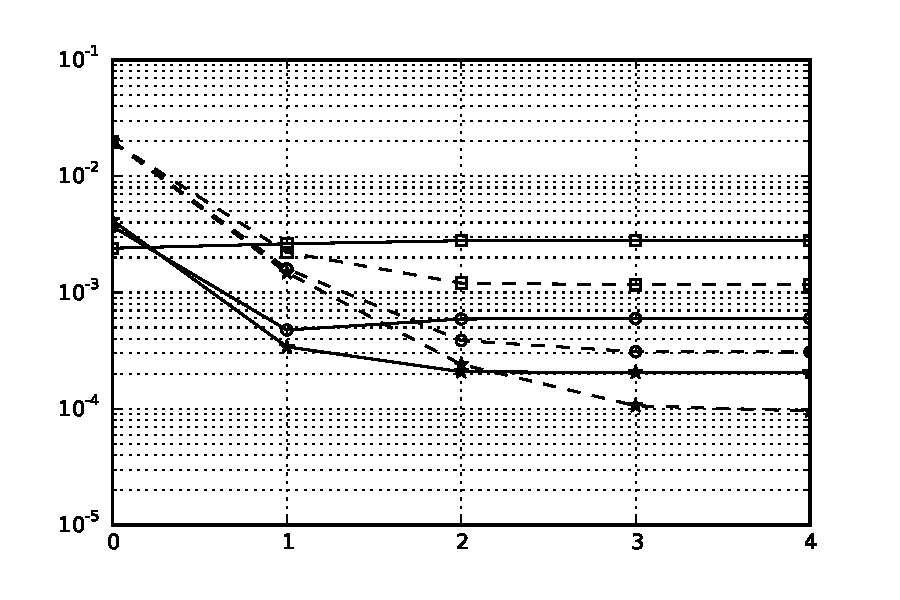
\includegraphics[width=0.8\textwidth]{UQAP/convergence1D}
  \bicaption[Fig:1]{例一:$\rho$均值的误差(实线)和标准差的误差(虚线)与gPC阶数的关系。这里$\eps = 10^{-8}$: $\Delta x = 0.04$(方形),$\Delta x = 0.02$(圆圈),$\Delta x = 0.01$(星号)。}{例一:$\rho$均值的误差(实线)和标准差的误差(虚线)与gPC阶数的关系。这里$\eps = 10^{-8}$: $\Delta x = 0.04$(方形),$\Delta x = 0.02$(圆圈),$\Delta x = 0.01$(星)。}{Fig}{Example 1. Errors of the mean (solid line) and standard deviation (dash line) of $\rho$ with respect to the gPC order at $\eps = 10^{-8}$: $\Delta x = 0.04$ (squares), $\Delta x = 0.02$ (circles), $\Delta x = 0.01$ (stars).}
\end{figure}

在图\ref{Fig:1}中,我们绘制了gPC数值解的均值和标准偏差的误差在$t = 0.01$与gPC阶数关系。三组结果包括:$\Delta x = 0.04$(正方形),$\Delta x = 0.02$(圆圈),$\Delta x = 0.01$(星)。这里$\Delta t = 0.0002 / 3$。可以看到,误差随着$N$增大快速衰减,然后在空间离散误差占优势变缓。很明显,即使$\eps = 10^{-8}$,由gPC展开导致的误差在$M = 4$时就可以被忽略。解的均值和标准偏差的曲线分别显示在图\ref{Fig:2}的左边和右边。

图\ref{Fig:6}中我们还绘制了的通量$vf$的平均值和标准偏差的曲线。在这里我们观察到gPC-SG方法和配点法以及参考解(\ref{limiting solution})之间良好的一致性。
\begin{figure}[htbp]
  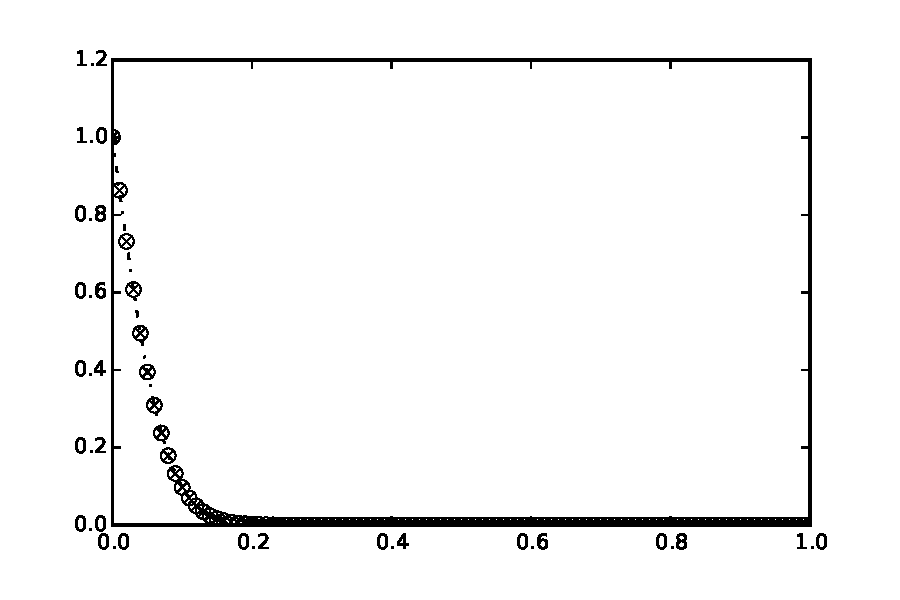
\includegraphics[width=0.5\textwidth]{UQAP/mean1D}
  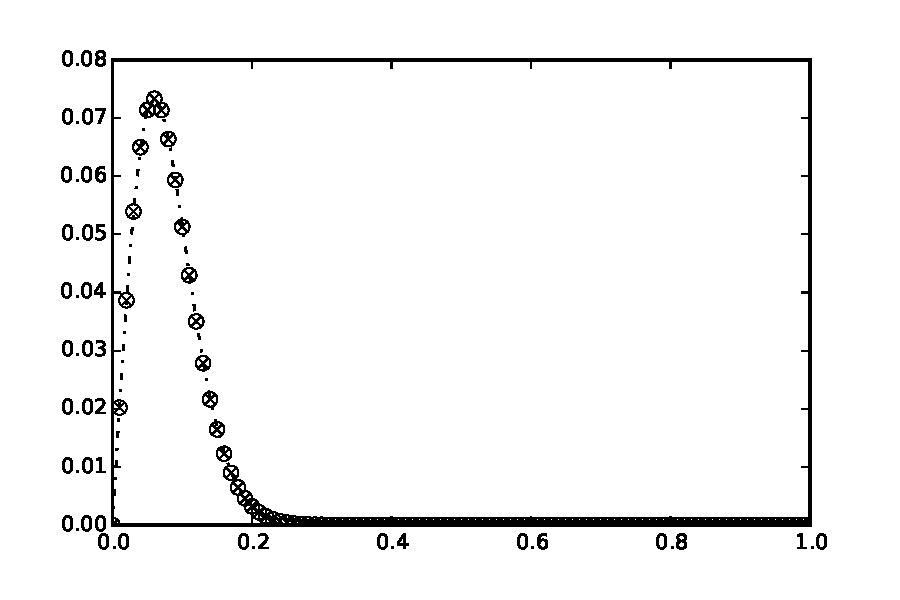
\includegraphics[width=0.5\textwidth]{UQAP/std1D}
  \bicaption[Fig:2]{例一:$\rho$的均值(左)和标准差(右)。$ \eps = 10 ^ {-8}$,gPC-SG方法$M = 4$(圆圈),配点法(叉)和极限解析解(\ref{limiting solution})。}{例一:$\rho$的均值(左边)和标准差(右边)。$ \eps = 10 ^ {-8}$,gPC-SG方法$M = 4$(圆圈),配点法(叉)和极限解析解(\ref{limiting solution})。}{Fig}{Example 1. The mean (left) and standard deviation (right) of $\rho$ at $\eps=10^{-8}$, obtained by the gPC Galerkin at order $M=4$ (circles), the stochastic collocation method (crosses), and the limiting analytical solution~(\ref{limiting solution}).}
\end{figure}
\begin{figure}[htbp]
  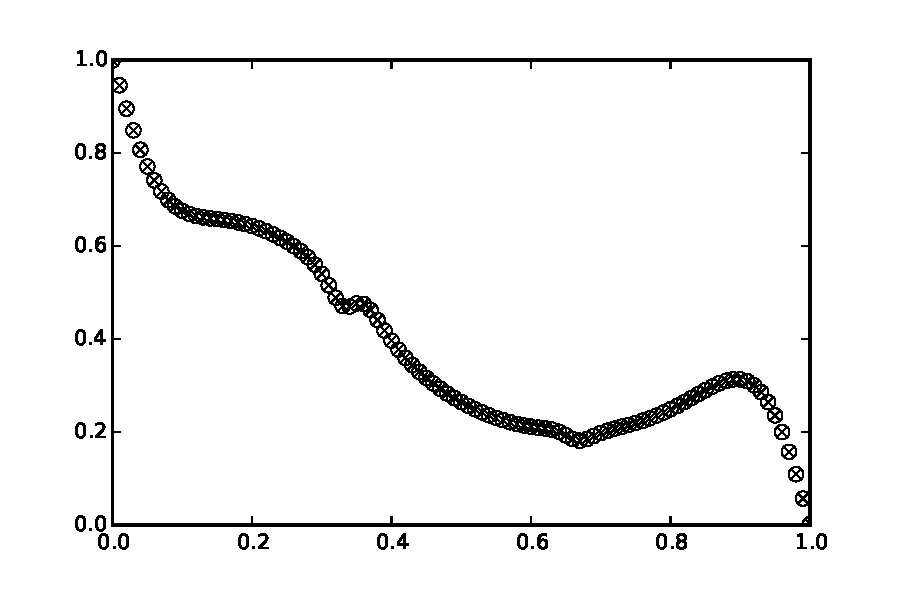
\includegraphics[width=0.5\textwidth]{UQAP/mean1D001}
  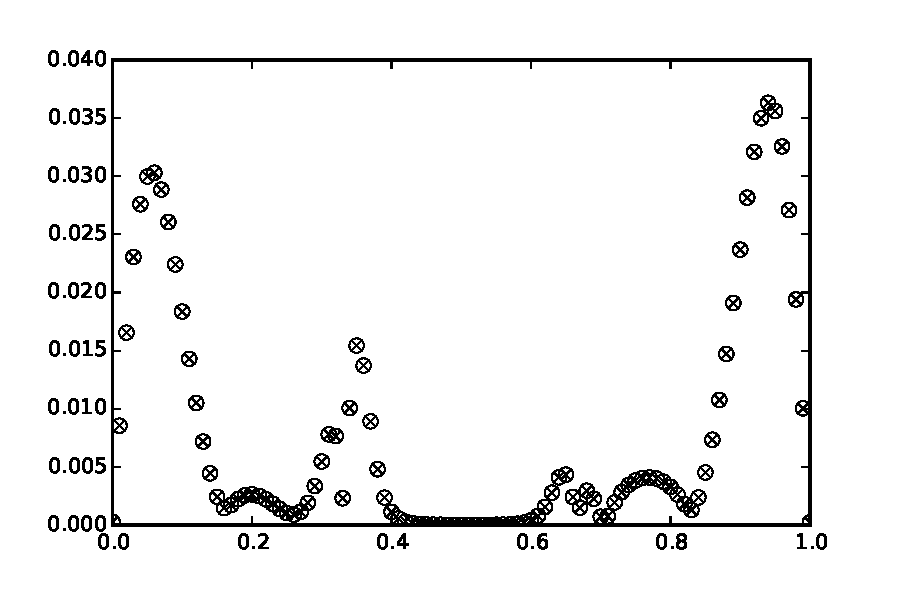
\includegraphics[width=0.5\textwidth]{UQAP/std1D001}
  \bicaption[Fig:6]{例一:均值(左)和标准差(右),gPC-SG方法(圆圈)和配点法(叉),$t=0.01$。}{例一:均值(左)和标准差(右),gPC-SG方法(圆圈)和配点法(叉),$t=0.01$。}{Fig}{Example 1. The mean (left) and standard deviation (right) obtained by gPC-Galerkin (circle) and collocation method (cross) at time $t=0.01$}
\end{figure}
\begin{figure}[htbp]  
  \centering
  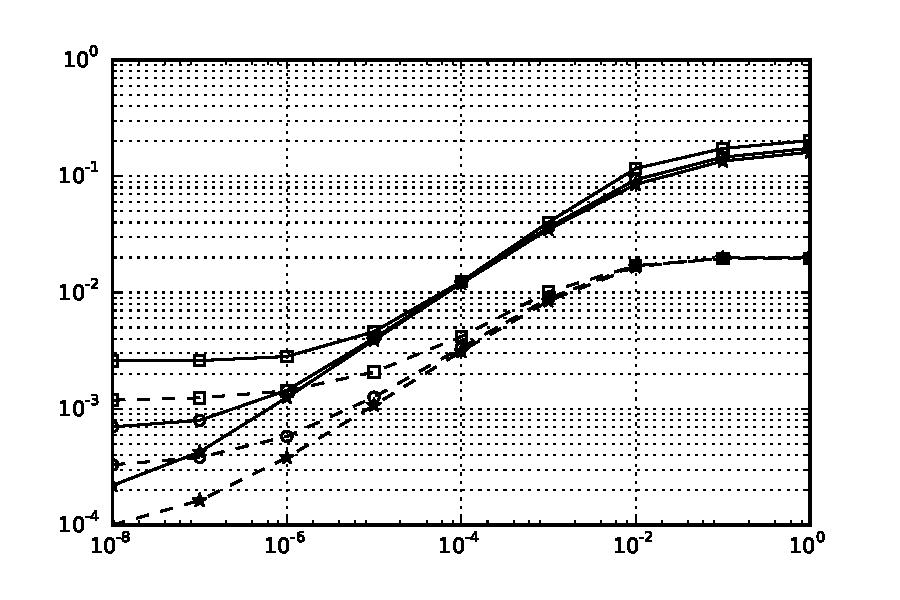
\includegraphics[width=0.8\textwidth]{UQAP/EPS_1D}
  \bicaption[Fig:3]{例一:两种解:解析解(\ref{limiting solution})和四阶gPC-SG方法,$\rho$的均值误差(实线)和标准差误差(虚线)与$\eps^2$的关系。$\Delta x = 0.04$ (方形), $\Delta x = 0.02$ (圆圈) and $\Delta x = 0.01$ (星)。}{例一:两种解:解析解(\ref{limiting solution})和四阶gPC-SG方法,$\rho$的均值误差(实线)和标准差误差(虚线)与$\eps^2$的关系。$\Delta x = 0.04$ (方形), $\Delta x = 0.02$ (圆圈) and $\Delta x = 0.01$ (星)。}{Fig}{Example 1. Differences in the mean (solid line) and standard deviation (dash line) of $\rho$ with respect to $\eps^2$, between the limiting analytical solution(\ref{limiting solution}) and the 4th-order gPC solution with $\Delta x = 0.04$ (squares), $\Delta x = 0.02$ (circles) and $\Delta x = 0.01$ (stars).}
\end{figure}

在图\ref{Fig:3}中,我们检查由四阶gPC-SG方法获得的解在$t = 0.01$时$\Delta x = 0.01$,$\Delta t = \Delta x^2/12$与极限方程解析解(\ref{limiting solution})的误差。正如预期,在数值误差占主导之前当$\eps^2$变小的时候误差会随之变小。
\subsection{例二:混合尺度}
在这个测试中,我们仍然令$\sigma = 2 + z$。考虑如果$\eps>0$也在一个较大的混合尺度上依赖于空间变量:
\begin{equation}
\eps(x)=10^{-3}+\frac{1}{2}[\tanh(6.5-11x)+\tanh(11x-4.5)]
\end{equation}
并光滑地从$O(10^{-3})$变到$O(1)$,如图\ref{Fig:7}。这种情况下会验证我们格式在混合多尺度下的适应能力,尤其是关于$\eps$的一致收敛性。
\begin{figure}[htbp]
  \centering
  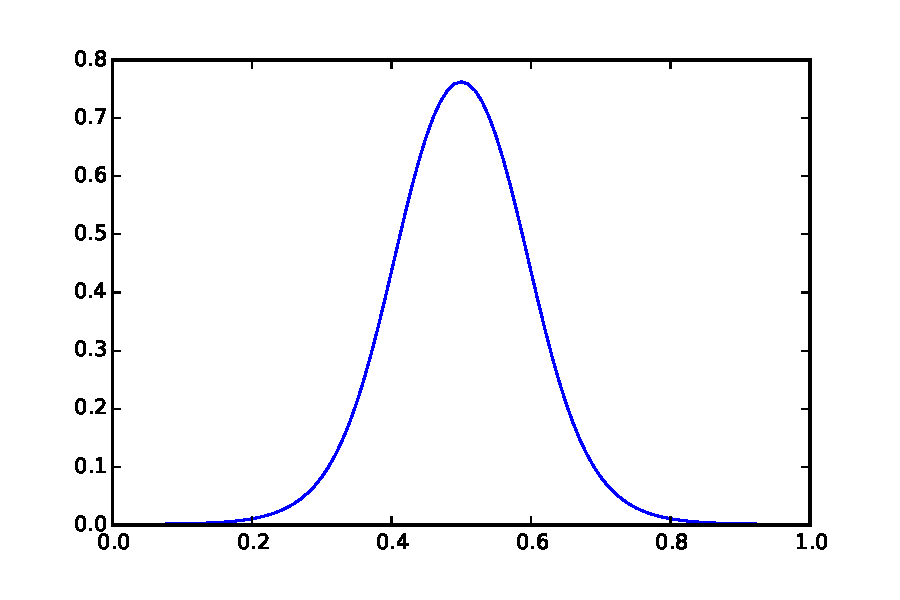
\includegraphics[width=0.8\textwidth]{UQAP/epsilon}
  \bicaption[Fig:7]{$\eps(x)$}{$\eps(x)$}{Fig}{$\eps(x)$}
\end{figure}

为了使质量仍然守恒,正确的线性输运方程为如下的形式,
\begin{equation}
  \dt f + v \dx\Big(\frac{1}{\varepsilon(x)} f\Big) = \frac{\sigma}{\eps^2(x)}{\cal L} f - \sigma^a f + S, \qquad \sigma(x, z) \ge \sigma_{\text{min}} > 0,
\end{equation}
那么micro-macro分解(\ref{eq-mM})修改为
\begin{subequations}
  \begin{align}
    & \dt \rho + \dx\av{vg} = -\sigma^a \rho + S ,  \\
    & \dt g + \frac{1}{\eps(x)} (I-\av{.}) (v\dx g) = -\frac{\sigma(z)}{\eps^2(x)}g  - \sigma^a g - \frac{1}{\eps(x)}v \dx\Big(\frac{1}{\varepsilon(x)}\rho\Big).
  \end{align}
\end{subequations}
可以发现只有最后一项发生了变化。对于极限方程(\ref{eq-diff1}),也需要修改为
\begin{equation}
  \dt \rho =  \partial_{x} (\kappa(z)  \partial_{x}\rho) - \dx(\kappa(z)a(x)\rho)-\sigma^a(z) \rho +S,
\end{equation}
其中我们假设
\begin{equation}
  a(x) =\lim\limits_{\varepsilon\rightarrow 0}\frac{\varepsilon'(x)}{\varepsilon(x)},
\end{equation}
存在。对于相应的数值格式,我们也只需要把(\ref{eq-schg})中的最后一项
\begin{equation}
  -\frac{1}{\eps^2}v\frac{\hrhonip-\hrhoni}{\Dx}
\end{equation}
替换为
\begin{equation}
   -\frac{1}{\eps(x_{i+1/2})}v\Bigg(\frac{\hrhonip}{\eps(x_{i+1})}-\frac{\hrhoni}{\eps(x_i)}\Bigg)\frac{1}{\Dx}.ß
\end{equation}

初值为
\begin{equation}\label{eg2-ini1}
f_{\text{in}}(x,v,z)=\frac{\rho_0}{2}\big [\exp\big(-(\frac{v-0.75}{T_0})^2\big)+\exp\big(-(\frac{v+0.75}{T_0})^2\big)\big ]
\end{equation}
其中
\begin{equation}\label{eg2-ini2}
\rho_0(x)=\frac{2+\sin(2\pi x)}{2},\quad T_0(x)=\frac{5+2\cos(2\pi x)}{20}.
\end{equation}

参考解是由配点法(30样本)得到。相关参数如下:网格空间$\Delta x = 0.01$,时间$\Delta t = \Delta x^2/3$。我们用五阶gPC-SG方法分别演化到时刻$t=0.005$,$t=0.01$, $t=0.05$, $t=0.1$。对于$v$方向的积分,我们使用30个点的高斯积分。

图\ref{Fig:8}显示了均值和标准差的$\ell^2$误差与gPC阶数的关系,可以看出收敛的非常快(谱收敛)。
\begin{figure}[htbp]
  \centering
  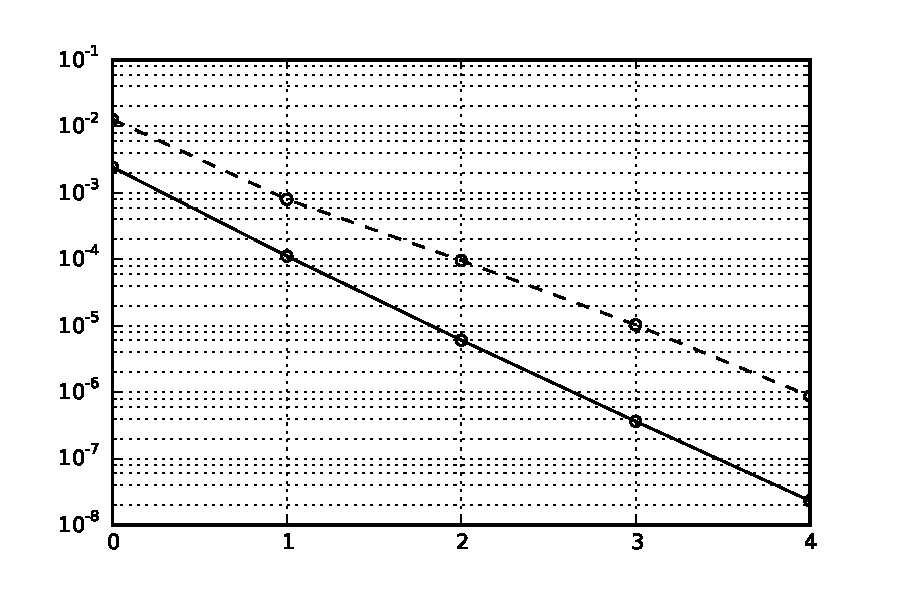
\includegraphics[width=0.8\textwidth]{UQAP/convergence1Deps}
  \bicaption[Fig:8]{例二:均值(实线)和标准差(虚线)的$\ell^2$误差与gPC阶数的关系}{例二:均值(实线)和标准差(虚线)的$\ell^2$误差与gPC阶数的关系}{Fig}{Example 2 with initial data(\ref{eg2-ini1})--(\ref{eg2-ini2}). The $\ell^2$ error of mean and standard deviation (dash line) with respect to gPC order. }
\end{figure}

\subsection{例三:随机初值}
接下来我们在初值上加入随机性($\sigma=2+z$仍然随机)。
\begin{equation}
f(0,x,v,z) = f(0,x,v)+0.2z
\end{equation}
其中$f(x,v,0)$和(\ref{eg2-ini1})中一样。这次$\Dx=0.01$,$\Delta t = \Delta x^2/12$以及最终时间$T=0.01$。首先我们测试流体极限$\varepsilon=10^{-8}$,如图\ref{Fig:9}。
\begin{figure}[htbp]
  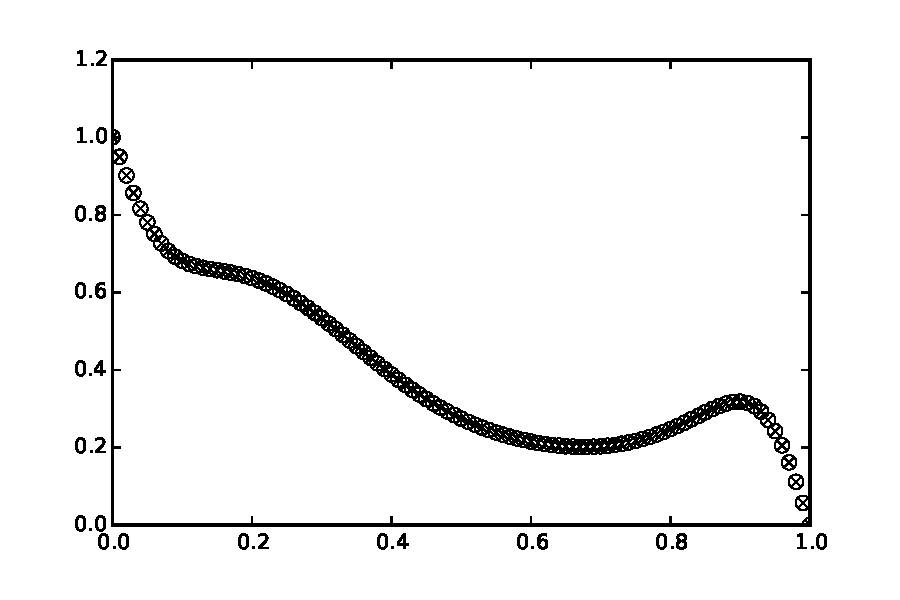
\includegraphics[width=0.5\textwidth]{UQAP/mean1Dir}
  \includegraphics[width=0.5\textwidth]{UQAP/std1Dir}
  \bicaption[Fig:9]{例三:均值(左)和标准差(右),gPC-SG方法(圆圈)和配点法(叉),$t=0.1$,$\varepsilon=10^{-8}$。}{例三:均值(左)和标准差(右),gPC-SG方法(圆圈)和配点法(叉),$t=0.1$,$\varepsilon=10^{-8}$。}{Fig}{Example 3. The mean (left) and standard deviation (right) obtained by gPC-Galerkin (circle) and collocation method (cross) at time $t=0.1$, $\varepsilon=10^{-8}$.}
\end{figure}
接下来我们测试$\varepsilon=1$,如图\ref{Fig:10}。
\begin{figure}[htbp]
  \includegraphics[width=0.5\textwidth]{UQAP/mean1DirO1}
  \includegraphics[width=0.5\textwidth]{UQAP/std1DirO1}
  \bicaption[Fig:10]{例三:均值(左)和标准差(右),gPC-SG方法(圆圈)和配点法(叉),$t=0.1$, $\varepsilon=1$。}{例三:均值(左)和标准差(右),gPC-SG方法(圆圈)和配点法(叉),$t=0.1$, $\varepsilon=1$。}{Fig}{Example 3. The mean (left) and standard deviation (right) obtained by gPC-Galerkin (circle) and collocation method (cross) at time $t=0.1$, $\varepsilon=1$}
  % \label{Fig:10}
\end{figure}
可以看到两种方法吻合度很高。

\subsection{例四:随机边界条件}
这个例子中,我们在边界条件中加入随机性:
\begin{equation}
f_L(t,v,z) = 2 + z,\quad f_R(t,v,z) = 1 + z.
\end{equation}
我们也测试了当$\varepsilon=10^{-8}$和$\varepsilon=10$两种情况,如图\ref{Fig:11}和图\ref{Fig:12},同样的gPC-SG方法和参考解高度吻合。
\begin{figure}[htbp]
  \includegraphics[width=0.5\textwidth]{UQAP/mean1Dbr}
  \includegraphics[width=0.5\textwidth]{UQAP/std1Dbr}
  \bicaption[Fig:11]{例四:均值(左)和标准差(右),gPC-SG方法(圆圈)和配点法(叉),$t=0.1$, $\varepsilon=10^{-8}$。}{例四:均值(左)和标准差(右),gPC-SG方法(圆圈)和配点法(叉),$t=0.1$, $\varepsilon=10^{-8}$。}{Fig}{Example 4. The mean (left) and standard deviation (right) obtained by gPC-Galerkin (circle) and collocation method (cross) at time $t=0.1$, $\varepsilon=10^{-8}$}
\end{figure}
\begin{figure}[htbp]
  \includegraphics[width=0.5\textwidth]{UQAP/mean1DbrO10}
  \includegraphics[width=0.5\textwidth]{UQAP/std1DbrO10}
  \bicaption[Fig:12]{例四:均值(左)和标准差(右),gPC-SG方法(圆圈)和配点法(叉),$t=0.1$, $\varepsilon=10$。}{例四:均值(左)和标准差(右),gPC-SG方法(圆圈)和配点法(叉),$t=0.1$, $\varepsilon=10$。}{Fig}{Example 4. The mean (left) and standard deviation (right) obtained by gPC-Galerkin (circle) and collocation method (cross) at time $t=0.1$, $\varepsilon=10$}
\end{figure}


\subsection{例五:二维随机空间}
最后,我们来考察具有如下形式的二维随机场:
\begin{equation}
  \sigma(x,z_1,z_2) = 1 - \frac{\sigma z_1}{\pi^2}\cos(2\pi x) - \frac{\sigma z_2}{4\pi^2}\cos(4\pi x)
\end{equation}
% where we set $\sigma=4$ and $z_1, z_2$ are both uniformly distributed in $(-1,1)$. The mean and standard deviation of the solution $\rho$ at $t=0.01$ obtained by the 5th-order gPC Galerkin with $\Delta x = 0.025$, $\Delta t = 0.0002/3$ are shown in Figure\ref{Fig:4}. We then use the high-order stochastic collocation  method over 40$\times$40 Gauss-Legendre quadrature points to compute the reference mean and standard deviation of the solutions. In Figure\ref{Fig:5}, we show the errors of the mean (solid lines) and standard deviation (dash lines) of $\rho$ with respect to the order of gPC expansion. The fast spectral convergence of the errors can be clearly seen.

其中我们设置$\sigma = 4$和$z_1,z_2$为均匀分布在$(-1,1)$上的随机变量。由$\Delta x = 0.025$,$\Delta t = 0.0002 / 3$的五阶gPC-SG方法得到在$t = 0.01$的解$\rho$的均值和标准偏差见图\ref{Fig:4}。然后我们使用高阶配点法(40$\times$40高斯 - 勒让德积分点)来计算解的参考解的均值和标准差。在图\ref{Fig:5}中,我们画出$\rho$的均值(实线)和标准差(虚线)的误差与gPC阶数的关系。可以清楚地看到误差的快速谱收敛。
\begin{figure}[H]  
  \includegraphics[width=0.5\textwidth]{UQAP/mean2D}
  \includegraphics[width=0.5\textwidth]{UQAP/std2D}
  \bicaption[Fig:4]{均值(左)和标准差(右),五阶gPC-SG方法(圆圈)和配点法(叉),二维随机变量。}{均值(左)和标准差(右),五阶gPC-SG方法(圆圈)和配点法(叉),二维随机变量。}{Fig}{The mean (left) and standard deviation (right) of $\rho$ at $\eps = 10^{-8}$, obtained by 5th-order gPC Galerkin (circles) and the stochastic collocation method (crosses). The random input has dimension $d=2$.}
\end{figure}
\begin{figure}[H]  
  \centering
  \includegraphics[width=0.8\textwidth]{UQAP/convergence2D}
  \bicaption[Fig:5]{$\rho$的均值误差(实线)和标准差误差(虚线)与gPC-SG阶数的关系,二维随机变量。}{$\rho$的均值误差(实线)和标准差误差(虚线)与gPC-SG阶数的关系,二维随机变量。}{Fig}{Errors of the mean (solid line) and standard deviation (dash line) of $\rho$ with respect to gPC order, with the $d=2$ dimensional random input.}
\end{figure}


%\includegraphics[scale=.8]{mean.pdf}

%\includegraphics[scale=.8]{deviation.pdf}

%\includegraphics[scale=.8]{err_gpc_order_1.pdf}


%\includegraphics[scale=.8]{error_eps.pdf}

\section{本章总结与展望} \label{sec:conl}

在本章中,我们建立了随机伽辽金方法对带有随机散射系数的线性输运方程关于克努森数一致的谱精度分析,从而允许我们证明该方法具有随机渐近保持性质(s-AP)。对于基于micro-macro分解的全离散格式,我们证明了一致的稳定性结果。这是首次有人证明了关于这类问题的一致性结果。

关于一致性的分析在带有多尺度与不确定性的问题中非常重要。我们的分析对于线性问题具有一般的指导意义,进而可以推广到更多的kinetic方程或其他方程上去。而对于非线性的问题,仍然非常困难,将作为未来的研究的内容。


% \bibliographystyle{plain}
% \bibliography{UQAP_bibtex}

% \end{document}

% ==============

% We proceed in five short steps.

% \noindent {\it Step 1.} \\
% Here we derive a first energy relation. With the finite difference operators defined
% in(\ref{eq-diff_onesided})--(\ref{eq-diff_centered2}), our scheme can
% be written in the following compact form:
% \begin{subequations}\label{eq-cscheme}
%   \begin{align}
% & \frac{\hrhonpi-\hrhoni}{\Dt} + \Dnot\av{v\hgnp_i} = 0 \label{eq-srho}
% \\
% & \frac{\hgnpi-\hgni}{\Dt} + \frac{1}{\eps} (I-\av{.})
% \left(v^+\Dm+v^-\Dp\right)\hgni = - \frac{\Sigma}{\eps^2} \hgnpi
% - \frac{1}{\eps^2}v\,\dnot \hrhon_{i+\half}.\label{eq-sg}
%   \end{align}
% \end{subequations}


% We define the energy of system(\ref{eq-mM}) as $\int_\R \hat \rho^2 \, \diff x +
% \eps^2 \int \av{\hat g^2} \, \diff x$. It is clear that our scheme can be proved
% to be stable if the energy at time $n+1$ can be controlled by the
% energy at time $n$. Consequently, we first multiply(\ref{eq-srho}) by
% $\hrhonpi$, then we take the sum over $i\in\Z$, and finally, we use
% the standard equality $a(a-b)=\half(a^2-b^2+|a-b|^2)$ to get:
% \begin{subequations}
% \begin{equation}  \label{eq-Erho}
% \frac{1}{2\Dt} \left(  \rnorm{\hrhonp}^2- \rnorm{\hrhon}^2+\rnorm{\hrhonp-\hrhon}^2\right)
% + \sumi \hrhonpi\Dnot\av{v\hgnp_i}\Dx = 0.
% \end{equation}
% Second, we multiply(\ref{eq-sg}) by $\hgnpi$, we take the velocity
% average, we sum over $i\in \Z$, and we get:
% \begin{equation}  \label{eq-Eg}
% \begin{split}
% & \frac{1}{2\Dt} \left( \gnorm{\hgnp}^2-\gnorm{\hgn}^2 + \gnorm{\hgnp-\hgn}^2  \right)
% + \frac{1}{\eps}\innerp{\hgnp}{(I-\av{.})\left(v^+\Dm+v^-\Dp\right)\hgn} \\
% &  = - \frac1{\eps^2}  \langle \hgnp, {\hat \sigma} \hgnp \rangle - \frac{1}{\eps^2}\sumi \av{v\hgnpi}\dnot \hrhon_{i+\half}\Dx.
% \end{split}
% \end{equation}
% \end{subequations}
% $$
%    \langle \hgnp, \Sigma \hgnp \rangle \ge \sigma_m \gnorm{\hgnp}^2
% $$
% Now we use proposition\ref{prop:gav}: since $\av{\hgnpi}=0$ for every
% $i$, a simple expansion of the inner product of(\ref{eq-Eg}) shows
% that it can be reduced to:
% \begin{equation}  \label{eq-Innp}
% \begin{split}
% & \innerp{\hgnp}{(I-\av{.})\left(v^+\Dm+v^-\Dp\right)\hgn}   \\
% & =  \innerp{\hgnp}{\left(v^+\Dm+v^-\Dp\right)\hgn}
% -  \sumi \av{\hgnpi}\av{\left(v^+\Dm+v^-\Dp\right)\hgni}\Dx \\
% & = \innerp{\hgnp}{\left(v^+\Dm+v^-\Dp\right)\hgn}.
% \end{split}
% \end{equation}
% Consequently, we add up(\ref{eq-Erho}) and $\eps^2$
% times(\ref{eq-Eg}), then we use(\ref{eq-Innp}) and
% the discrete integration by parts of lemma\ref{lemma:intbp} to get our preliminary energy relation:
% \begin{equation}  \label{eq-ener}
% \begin{split}
% & \frac{1}{2\Dt} \left(  \rnorm{\hrhonp}^2-\rnorm{\hrhon}^2+\rnorm{\hrhonp-\hrhon}^2\right)
% + \sumi \hrhonpi\Dnot\av{v\hgnp_i}\Dx \\
% & + \frac{\eps^2}{2\Dt} \left( \gnorm{\hgnp}^2-\gnorm{\hgn}^2 +
%   \gnorm{\hgnp-\hgn}^2  \right) + \eps
% \innerp{\hgnp}{\left(v^+\Dm+v^-\Dp\right)\hgn} \\
% & \le  -\sigma_m \gnorm{\hgnp}^2 + \sumi \av{v\Dnot\hgnp_i} \hrhoni\Dx.
% \end{split}
% \end{equation}

% \bigskip
% \noindent {\it Step 2.} \\
% In this step, we show how the $\hrhonp-\hrhon$ term can be eliminated
% in(\ref{eq-ener}). First, it is useful to write $\hrhoni$ in the
% right-hand side of(\ref{eq-ener}) as $(\hrhoni-\hrhonpi)+\hrhonpi$:
% indeed, the terms $\sumi \hrhonpi\Dnot\av{v\hgnp_i}$ and $\sumi
% \av{v\Dnot\hgnp_i} \hrhonpi$ in the left and right-hand sides cancel
% out and we obtain:
% \begin{equation}  \label{eq-enerbis}
% \begin{split}
% & \frac{1}{2\Dt} \left(  \rnorm{\hrhonp}^2-\rnorm{\hrhon}^2+\rnorm{\hrhonp-\hrhon}^2\right) \\
% & + \frac{\eps^2}{2\Dt} \left( \gnorm{\hgnp}^2-\gnorm{\hgn}^2 +
%   \gnorm{\hgnp-\hgn}^2  \right) + \eps��
% \innerp{\hgnp}{\left(v^+\Dm+v^-\Dp\right)\hgn} \\
% & \le  -\sigma_m \gnorm{\hgnp}^2 + \sumi \av{v\Dnot\hgnp_i} (\hrhoni-\hrhonpi)\Dx.��
% \end{split}
% \end{equation}
% Now, we use
% the following Young inequality:
% \begin{equation}  \label{eq-Yrho}
% \sumi \av{v\Dnot\hgnp_i}(\hrhoni-\hrhonpi)\Dx \leq \alpha \rnorm{\hrhonp-\hrhon}^2
% +\frac{1}{4\alpha}\sumi\av{v\Dnot\hgnp_i}^2\Dx.
% \end{equation}

%  the $\hrhonp-\hrhon$ terms cancel out in(\ref{eq-enerbis}) if $\alpha=\frac{1}{2\Dt}$
% and we get
% \begin{equation}  \label{eq-fener}
% \begin{split}
% & \frac{1}{2\Dt} \left(  \rnorm{\hrhonp}^2-\rnorm{\hrhon}^2\right)
% + \frac{\eps^2}{2\Dt} \left( \gnorm{\hgnp}^2-\gnorm{\hgn}^2 +  \gnorm{\hgnp-\hgn}^2  \right) \\
% & + \eps \innerp{\hgnp}{\left(v^+\Dm+v^-\Dp\right)\hgn} \leq
% -\sigma_m \gnorm{\hgnp}^2 +\frac{\Dt}{2}\sumi\av{v\Dnot\hgnpi}^2\Dx.
% \end{split}
% \end{equation}


% \bigskip
% \noindent {\it Step 3.} \\
% Here, we work on the inner product of(\ref{eq-fener}) to show that
% the $\hgnp-\hgn$ terms can also be eliminated. First, we insert $\hgnp$
% in this inner product to get:
% \begin{equation}  \label{eq-vDgg1}
% \begin{split}
% & \innerp{\hgnp}{\left(v^+\Dm+v^-\Dp\right)\hgn}  \\
% & = \innerp{\hgnp}{\left(v^+\Dm+v^-\Dp\right)\hgnp}
%      + \innerp{\hgnp}{\left(v^+\Dm+v^-\Dp\right)(\hgn-\hgnp)} \\
% & = A+B,
% \end{split}
% \end{equation}
% and we rewrite terms $A$ and $B$ as follows. For $A$, we use the
% centered form of the upwind operator (lemma\ref{lemma:5}) and
% the discrete integration by parts of lemma\ref{lemma:intbp} to get:
% \begin{equation}\label{eq-vDgg2}
% \begin{split}
% A & = \innerp{\hgnp}{v\Dc\hgnp} -\frac{\Dx}{2} \innerp{\hgnp}{|v|\Dm\Dp\hgnp} \\
% &  = \frac{\Dx}{2} \innerp{\Dp\hgnp}{|v|\Dp\hgnp} \\
% & = \frac{\Dx}{2} \sumi \av{|v|\left(\Dp\hgnpi\right)^2}\Dx.
% \end{split}
% \end{equation}
% For $B$, we also use the discrete integration by parts of
% lemma\ref{lemma:intbp} to get:
% \begin{equation}\label{eq-vDgg3}
% \begin{split}
% B= -\innerp{\left(v^+\Dp+v^-\Dm\right)\hgnp}{\hgn-\hgnp}.
% \end{split}
% \end{equation}
% Then we apply the inequality of lemma\ref{lemma:3} to $B$ to get
% \begin{equation}  \label{eq-YB}
% |B|\leq \alpha \gnorm{\hgnp-\hgn}^2+\frac{1}{4\alpha}\gnorm{|v|\Dp\hgnp}^2.
% \end{equation}
% Therefore, using(\ref{eq-fener}),(\ref{eq-vDgg1}),(\ref{eq-vDgg2})
% and(\ref{eq-YB}), we see that the $\hgnp-\hgn$ terms cancel out
% in(\ref{eq-fener}) if $\alpha=\frac{\eps}{2\Dt}$, and we get
% \begin{equation}\label{eq-enera}
% \begin{split}
% & \frac{1}{2\Dt} \left(  \rnorm{\hrhonp}^2-\rnorm{\hrhon}^2\right)
% + \frac{\eps^2}{2\Dt} \left( \gnorm{\hgnp}^2-\gnorm{\hgn}^2 \right) \\
% & + \eps\frac{\Dx}{2} \sumi \av{|v|\left(\Dp\hgnpi\right)^2}\Dx
%   - \frac{\Dt}{2}\gnorm{|v|\Dp\hgnp}^2   \\
% & \leq   - \sigma_m \gnorm{\hgnp}^2 +\frac{\Dt}{2}\sumi\av{v\Dnot\hgnpi}^2\Dx.
% \end{split}
% \end{equation}

% \bigskip
% \noindent {\it Step 4.} \\
% Now, we show how all the $\Dp \hgnp$ and the $\Dnot \hgnp$ terms can be
% controlled by $\gnorm{\hgnp}$. First, note that the term
% $\frac{\Dt}{2}\gnorm{|v|\Dp\hgnp}^2$ of the left-hand side
% of(\ref{eq-enera}) can be estimated as follows:
% \begin{equation}\label{eq-majDg}
% \begin{split}
% \frac{\Dt}{2}\gnorm{|v|\Dp\hgnp}^2 & =  \frac{\Dt}{2} \sumi \av{|v|^2\left(\Dp\hgnpi\right)^2}\Dx \\
% & \leq \frac{\Dt}{2} \sumi \av{|v|\left(\Dp\hgnpi\right)^2}\Dx,
% \end{split}
% \end{equation}
% since $|v|\leq 1$. Moreover, using lemma\ref{lemma:2} and a change
% of indices shows that the
% last term of the right-hand side of(\ref{eq-enera}) satisfies
% \begin{equation}  \label{eq-majDnotg}
% \frac{\Dt}{2}\sumi\av{v\Dnot\hgnpi}^2\Dx \leq \frac{\Dt}{4}\sumi\av{|v|\left(\Dp\hgnpi\right)^2}\Dx.
% \end{equation}
% Finally, we use these two estimates in(\ref{eq-enera}) to obtain:
% \begin{equation}\label{eq-enerf}
% \begin{split}
% & \frac{1}{2\Dt} \left(  \rnorm{\hrhonp}^2-\rnorm{\hrhon}^2\right)
% + \frac{\eps^2}{2\Dt} \left( \gnorm{\hgnp}^2-\gnorm{\hgn}^2 \right)   \\
% & \leq  - \sigma_m\gnorm{\hgnp}^2 + \left(\frac{3\Dt}{4}- \eps\frac{\Dx}{2}\right) \sumi \av{|v|\left(\Dp\hgnpi\right)^2}\Dx.
% \end{split}
% \end{equation}
% Now, taking the positive part of the factor $(\frac{3\Dt}{4}- \eps\frac{\Dx}{2})$ of the
% right-hand side of(\ref{eq-enerf}), we have the estimate
% \begin{equation}\label{eq-enerfb}
% \begin{split}
%   \left(\frac{3\Dt}{4}- \eps\frac{\Dx}{2}\right) \sumi \av{|v|\left(\Dp\hgnpi\right)^2}\Dx
% & \leq   \left(\frac{3\Dt}{4}- \eps\frac{\Dx}{2}\right)^+ \sumi \av{\left(\Dp\hgnpi\right)^2}\Dx \\
% & \leq   \left(\frac{3\Dt}{4}- \eps\frac{\Dx}{2}\right)^+ \frac{4}{\Dx^2} \gnorm{\hgnp}^2,
% \end{split}
% \end{equation}
% where we have used $|v|\leq 1$ and the estimate of lemma\ref{lemma:estimDp}.


% \bigskip
% \noindent {\it Step 5.}  \\
% Finally, estimates(\ref{eq-enerf}) and(\ref{eq-enerfb}) show that
% \begin{equation*}
%    \frac{1}{2\Dt} \left(  \rnorm{\hrhonp}^2-\rnorm{\hrhon}^2\right)
% + \frac{\eps^2}{2\Dt} \left( \gnorm{\hgnp}^2-\gnorm{\hgn}^2 \right)
% \leq \left( \left(\frac{3\Dt}{4}- \eps\frac{\Dx}{2}\right)^+ \frac{4}{\Dx^2}-\sigma_m\right) \gnorm{\hgnp}^2.
% \end{equation*}
% This means that we have the final energy estimate
% \begin{equation*}
%   \rnorm{\hrhonp}^2+ \eps^2\gnorm{\hgnp}^2 \leq \rnorm{\hrhon}^2+ \eps^2\gnorm{\hgn}^2
% \end{equation*}
% if $\Dt$ is such that
% \begin{equation*}
%   \left(\frac{3\Dt}{4}- \eps\frac{\Dx}{2}\right)^+ \frac{4}{\Dx^2}\leq\sigma_m.
% \end{equation*}
% Since $\sigma_m > 0$, an equivalent condition is $(\frac{3\Dt}{4}- \eps\frac{\Dx}{2})
% \frac{4}{\Dx^2}\leq\sigma_m$, which gives the sufficient condition
% \begin{equation*}
%   \Dt\leq \frac{\Dx^2\sigma_m}{3} + \frac{2}{3}\eps\Dx,
% \end{equation*}
% which proves the theorem.


% !TeX root = ../thesis.tex

% \documentclass[preprint,3p]{elsarticle} 
% %\journal{J. Comput. Phys.}

% \usepackage{geometry}                		% See geometry.pdf to learn the layout options. There are lots.                		% ... or a4paper or a5paper or ... 
% \usepackage{graphicx}				% Use pdf, png, jpg, or eps§ with pdflatex; use eps in DVI mode
% \usepackage{wrapfig}
% \usepackage{amsmath,amssymb,amsthm}							% TeX will automatically convert eps --> pdf in pdflatex
% \usepackage{multirow}
% \usepackage{tabularx,epsfig,color,caption}
% \usepackage{algorithm,algorithmic,mathtools,bm}
% \usepackage{epstopdf}

%%%%%%%%%%%%%%%%% author macros %%%%w%%%%%%%%%
% \renewcommand{\theequation}{\arabic{section}.\arabic{equation}}  % numbering the equation by section
% \newtheorem{theorem}{THEOREM}[section]
% \newtheorem{remark}{Remark}[section]
% \newtheorem{lemma}{LEMMA}[section]
% \newtheorem{exmp}{Example}[section]
% \newcommand*\note[1]{{\color{red}{(NOTE: #1)}}}
% \newcommand*\todo[1]{{\color{red}{(TODO: #1)}}}

\newcommand{\be}{\begin{equation}}
\newcommand{\ee}{\end{equation}}
\newcommand{\ba}{\begin{array}}
\newcommand{\ea}{\end{array}}
\newcommand{\bea}{\begin{eqnarray}}
\newcommand{\eea}{\end{eqnarray}}
\newcommand{\beas}{\begin{eqnarray*}}
\newcommand{\eeas}{\end{eqnarray*}}


\newcommand\bR{\mathbb{R}}
\renewcommand{\bx}{{\bf x}}
\renewcommand{\by}{{\bf y}}
\renewcommand{\bk}{{\bf k}}
\renewcommand{\bz}{{\bf 0}}



% \begin{document}


% \begin{frontmatter}


% \title{An improved semi-Lagrangian time splitting spectral method for the semi-classical Schr\"odinger equation with vector potentials using NUFFT}
% \author[sjit]{Zheng MA}
% \ead{mayuyu@sjtu.edu.cn}

% \address[sjit]{Department of Mathematics,
% Shanghai Jiao Tong University,
% 800 Dongchuan RD, Shanghai, 200240, China}

% \author[irmar,wpi]{Yong ZHANG\corref{5}}
% \ead{yong.zhang@univ-rennes1.fr}
% \address[irmar]{Universit\'e de Rennes 1, IRMAR, Campus de Beaulieu, 35042 Rennes Cedex, France}
% \address[wpi]{Wolfgang Pauli Institute c/o Fak. Mathematik, University Wien, Oskar-Morgenstern-Platz 1, 1090 Vienna, Austria}

% \author[duke]{Zhennan ZHOU}
% \ead{zhennan@math.duke.edu}
% \address[duke]{Departments of Mathematics, Duke University, Box 90320, Durham, NC, 27708, USA}

% \cortext[5]{Corresponding author.}




% %%%%% Begin Abstract %%%%%%%%%%%
% \begin{abstract}
% In this paper, we propose a new time splitting Fourier spectral method for the semi-classical Schr\"{o}dinger equation with vector potentials. 
% Compared with the results in \citen{SemiJZ}, our method achieves spectral accuracy in space by interpolating the Fourier series via the 
% NonUniform Fast Fourier Transform (NUFFT) algorithm in the convection step.
% The NUFFT algorithm helps maintain high spatial accuracy of Fourier method, and at the same time improve the efficiency from $O(N^{2})$ (of direct computation) to $O(N\log N)$ operations, where $N$ is the total number of grid points.
% The kinetic step and potential step are solved by analytical solution with pseudo-spectral approximation,  and, 
% therefore, we obtain spectral accuracy in space for the whole method.  
% We prove that the method is unconditionally stable, and we show improved error estimates for both the wave function and physical observables, which agree with the results in \citen{BaoJM} for vanishing potential cases and are superior to those in  \citen{SemiJZ}.
% Extensive one and two dimensional numerical studies are presented to verify the properties of the proposed method, and simulations of 3D problems are demonstrated to show its potential for  future practical applications.

% \end{abstract}



% \begin{keyword}
% semi-classical Schr\"{o}dinger equation, vector potential, semi-Lagrangian time splitting method, nonuniform FFT
% \end{keyword}


% \end{frontmatter}

\chapter{使用NUFFT的半拉格朗日时间算子分裂法在具有向量势的薛定谔方程的应用}

%------------------------------------------------------
%\section{简介}
%\subsection{Background and outline}

% Quantum effects play a significant role in many scientific and engineering areas, such as theoretical chemistry, solid-state mechanics and quantum optics, and the mathematical analysis and numerical simulation of Schr\"{o}dinger equations 
% are of fundamental importance. This type of equations form a canonical class of dispersive PDEs, i.e., equations where waves of different wavelengths propagate at different phase velocities. Whenever the magnetic field is considered,  we need to incorporate the vector potentials in the  Schr\"{o}dinger equation.

量子效应在许多科学和工程领域中发挥重要作用,例如理论化学,固态力学和量子光学。而对于薛定谔方程的数学分析和数值模拟具有根本的重要性。这种类型的方程形成了一类的色散偏微分方程,即不同波长的波在不同相速度下传播的方程。而当考虑磁场时,我们需要将向量势函数引入到薛定谔方程中。

% In this paper, we consider the semi-classical Schr\"odinger equation with vector potentials, which has the form
在本章中,我们考虑具有向量势函数的半经典薛定谔方程,其具有形式
\begin{equation} \label{eq:main1}
i\varepsilon\partial_{t}u^{\varepsilon}=\frac{1}{2}\left(-i\varepsilon\nabla_x-\mathbf{A}(x)\right)^{2}u^{\varepsilon}+V(x)u^{\varepsilon},\quad t\in\mathbb{R}^{+},\quad x\in\mathbb{R}^{3},
\end{equation}
\begin{equation}
u^{\varepsilon}({x},0)=u_{0}({x}),\quad x \in\mathbb{R}^{3}\label{eq:initial cond},
\end{equation}
% where $u^{\varepsilon}({x},t)$ is the complex-valued
% wave function, $V({x})\in\mathbb{R}$  is the scalar potential and $\mathbf{A}({x})\in\mathbb{R}^{3}$
% is the vector potential. The scalar potential  and the vector
% potential  are introduced to mathematically describe the electromagnetic field, i.e., the electric
% field $\mathbf{E}({x})\in\mathbb{R}^{3}$ and the magnetic
% field $\mathbf{B}({x})\in\mathbb{R}^{3}$ given as follows
其中$u^{\varepsilon}({x},t)$是复值波函数,$V({x})\in\mathbb{R}$是标量势函数,$\mathbf{A}({x})\in\mathbb{R}^{3}$是向量势函数。数学上我们用标量势和向量势来描述电磁场,即电场$\mathbf{E}({x})\in\mathbb{R}^{3}$和磁场$\mathbf{B}({x})\in\mathbb{R}^{3}$如下
\begin{equation}
\mathbf{E}=-\nabla V(x),\qquad\mathbf{B}=\nabla\times\mathbf{A}\left( x \right).
\end{equation}


% The Schr\"{o}dinger equation \eqref{eq:main1}
% above can be derived from the equation in the absence of the vector potential
% by local gauge transformation (see \citen{QO}). The quantum dynamics in the presence of the external
% electromagnetic field results in many far-reaching consequences in
% quantum mechanics, such as Landau levels, Zeeman effect and superconductivity.
% In the aspect of analysis, the Hamiltonian has different features in spectral and scattering properties (see
% \citen{magstudy}). Numerically, it gives new challenges as well,
% especially in the semi-classical regime. The presence of the vector
% potential introduces a convection term in the Schr\"{o}dinger
% equation and in the meanwhile effectively modifies the scalar potential
% (see \citen{SemiJZ}).
薛定谔方程\eqref{eq:main1}可以由不带向量势的方程通过局部规范变换(参见\citen{QO})导出。外部电磁场的存在的量子力学演化会导致许多深远的结果,例如朗道能级、塞曼效应和超导性。
在分析方面,哈密顿算子在光谱和散射性质上具有不同的特征(见\citen{magstudy})。数值上,它也带来了新的挑战,特别是在半经典格式中。向量势函数的存在使得薛定谔方程中引入对流项
并且同时标量势函数也产生了一定影响(参见\citen{SemiJZ})。


% In fact, one can simplify the potential description by imposing one
% more condition, namely, specifying the gauge. The electric field $\mathbf{E}(x)\in\mathbb{R}^{3}$
% and magnetic field $\mathbf{B}(x)\in\mathbb{R}^{3}$ stay invariant
% in different gauges. One natural choice is, $\nabla_{x}\cdot\mathbf{A}=0$, which is the so-called
% Coulomb gauge. In this gauge, the vector potential and the canonical
% momentum operator commute, $[\mathbf{A},\,-i\varepsilon\nabla_x]=0$,
% so that the modified ``kinetic'' part of the Schr$\ddot{\textrm{o}}$dinger
% equation \eqref{eq:main1} can be simplified  as follows
事实上,可以通过额外添加一个条件来简化势函数,即给出一个指定的规范。电场$\mathbf{E}(x)\in\mathbb{R}^{3}$
和磁场$\mathbf{B}(x)\in\mathbb{R}^{3}$具有所谓的规范不变性。一个自然的选择是$\nabla_{x}\cdot\mathbf{A}=0$,这就是所谓的库仑规范。在这个规范中,矢量势和正则动量互为对易,$[\mathbf{A},\,-i\varepsilon\nabla_x]=0$
使得修改后的薛定谔方程\eqref{eq:main1}的动能(``kinetic'')部分可以简化为如下
\begin{equation}\label{eq:reform}
\frac{1}{2}(-i\varepsilon\nabla_{x}-\mathbf{A})^{2}u^{\varepsilon}=-\frac{\varepsilon^{2}}{2}\Delta_{x}u^{\varepsilon}+i\varepsilon\mathbf{A}\cdot\nabla_{x}u^{\varepsilon}+\frac{1}{2}|\mathbf{A}|^{2}u^{\varepsilon}.
\end{equation}


% In the Schr$\ddot{\textrm{o}}$dinger equation, the wave function acts as an auxiliary quantity used to compute macroscopic physical quantities (physical observables)
% such as the position density
在薛定谔方程中,波函数作为辅助量用于计算宏观物理量(物理可观测量),例如位置密度
\begin{equation}
n(x,t)=|u^{\varepsilon}(x,t)|^{2},
\end{equation}
和修正的电流密度
\begin{equation}
\mathbf{J}(x,t)=\frac{1}{2}\left(\overline{u^{\varepsilon}}\left(-i\varepsilon\nabla_{x}-{\mathbf A}\right)u^{\varepsilon}-
u^{\varepsilon}\left(-i\varepsilon\nabla_{x}-{\mathbf A}\right)\overline{u^{\varepsilon}}\right),
\end{equation}
% where $\bar{f}$ denotes the complex conjugate of $f$. Actually, we have the following mass conservation equation
其中$\bar{f}$表示$f$的复共轭。实际上,我们有以下质量守恒方程
\begin{equation}
\frac{\partial}{\partial t}n+\nabla_{x}\cdot\mathbf{J}=0.
\end{equation}
% We remark that $n$ and $\mathbf{J}$ are gauge invariant quantities. Another two important physical quantities are the {\it mass}
我们指出$n$和$\mathbf{J}$都是规范不变量。另外两个重要的物理量是{\it 质量}
\begin{equation}
m(t):=\|u^{\varepsilon}(x,t)\|^2_{L^2}=\int_{\mathbb R^3} n(t,x) dx,
\end{equation}
和{\it 能量}
\begin{equation}
\mathcal E(t):=\frac{1}{2}\|(-i\varepsilon\nabla-\mathbf{A})u^{\varepsilon}\|_{L^2}^2+\langle u^{\varepsilon},Vu^{\varepsilon}\rangle,
\end{equation}
% where $\langle f,g\rangle \equiv\int_{\mathbb{R}^d}f(x)\overline{ g(x)}\,dx$ is the standard inner product. For $u^\varepsilon \in C(\mathbb{R}_t;L^2(\mathbb{R}^d) \cap \mathcal S (\mathbb R^d))$, these quantities are conserved through dynamics. We refer the readers to appendixes for detailed proofs.
其中$\langle f,g\rangle \equiv\int_{\mathbb{R}^d}f(x)\overline{ g(x)}\,dx$是标准的内积。对于$u^\varepsilon \in C(\mathbb{R}_t;L^2(\mathbb{R}^d) \cap \mathcal S (\mathbb R^d))$,这些量在动力学演化中是守恒的。我们把详细的证明放在本章的附录\ref{app_nufft}中。


% In the semi-classical regime, namely $\varepsilon \ll 1$, the wave function  $u^{\varepsilon}$ is highly oscillatory both in space and time on the scale
% $O(\varepsilon)$, therefore it does not converge in the strong sense as $\varepsilon\rightarrow0$. When $\varepsilon\ll1$, several approximate methods
% other than directly solving the Schr\"{o}dinger equation have been proposed, such as the level
% set method and the moment closure method based on the WKB analysis and the Wigner transform, see, for example, \citen{high_freq_waves,level_set,multi-phase,reviewsemiclassical}.
% The Gaussian beam method (or the Gaussian wave packet approach) is
% another important one, which allows accurate computation around caustics and captures phase information (see, for example, \citen{Ejheller,Popov,Gaussian_propagation,EGB}) with $O(\varepsilon^{1/2})$ model error.
% To improve the approximation accuracy, higher order Gaussian beam methods were introduced with an error $C_{k}(T)\varepsilon^{k/2}$
% (see \citen{HGBT,HEGB}). However, it has been shown in \citen{ErrorestiGB,HagedornV}
% that, for fixed $\varepsilon$, higher order Gaussian beam methods may not be a practical way to reduce the error. 
% Whereas, the Hagedorn wave packets, studied by Hagedorn \citen{Hagedornraising}, analyzed and implemented as a computational tool in \citen{Hagedornraising,Newsplitting,HagedornV}, 
% can effectively reduce the error for all $\varepsilon\in(0,1]$. In \citen{HagedornV}, Zhou has extended this method to the vector potential case and provided a rigorous proof for the higher order convergence with the Galerkin approximation. 
% Recently, Russo and Smereka in \citen{GBTrans,GBTrans2} proposed a new approach based on the so-called Gaussian Wave packet transform, which is another worthy alternative.

在半经典格式下,即$\varepsilon \ll 1$时,波函数$u^{\varepsilon}$在空间和时间上都是高度振荡的,振荡的尺度为$O(\varepsilon)$。因此当$\varepsilon\rightarrow0$时,它在强意义下并不收敛。当$\varepsilon\ll 1$时,相比于直接求解薛定谔方程,更多的是一些近似方法,如水平集方法和基于WKB分析和Wigner变换的矩封闭方法,参见\citen{high_freq_waves,level_set,multi-phase,reviewsemiclassical}。
高斯波束法(或高斯波包法)是另一类重要的方法,它允许精确计算焦散和捕获相位信息(参见例如\citen{Ejheller,Popov,Gaussian_propagation,EGB}),这种模型误差为$O(\varepsilon^{1/2})$。
为了提高近似精度,人们引入了高阶高斯波束方法,其具有误差$C_{k}(T)\varepsilon^{k/2}$
(见\citen{HGBT,HEGB})。然而,在\citen{ErrorestiGB,HagedornV}中已经证明
对于固定的$\varepsilon$,更高阶的高斯波束方法可能不是减少误差的实用方法。然而,Hagedorn在\citen{Hagedornraising}中提出,在\citen{Hagedornraising,Newsplitting,HagedornV}中分析和实现的Hagedorn波包
可以有效地减少所有$\varepsilon\in(0,1]$中的误差。在\citen{HagedornV}中,Zhou已经将该方法扩展到向量势函数,并为伽辽金近似的高阶收敛提供了严格的证明。
最近,Russo和Smereka在文献\citen{GBTrans,GBTrans2}中提出了一种基于所谓的高斯波包变换的新方法,这是另一个值得选择的方法。

% Numerically, if one wants to directly simulate the Schr\"{o}dinger equation \eqref{eq:main1},
% the oscillatory nature of the wave function gives rise to significant computational
% burdens. The computation of physical observables, like $n(x,t)$ and $\mathbf{J}(x,t)$, faces the same
% challenges. To our best knowledge, one of the best methods is the time splitting spectral method, introduced by Bao, Jin and Markowich
% in \citen{BaoJM,BaoJM2,reviewsemiclassical}, where the meshing strategy $\Delta t=O(\varepsilon)$ and $\Delta x=O(\varepsilon)$ is sufficient to guarantee an accurate approximation of the wave function.
% To compute correct physical observables, the time step can be relaxed to $O(1)$.

在数值上,如果想直接模拟薛定谔方程\eqref{eq:main1},波函数的振荡性质会使计算开销十分巨大。对于物理可观测量的计算,如$n(x,t)$和$\mathbf{J}(x,t)$,
也是如此。据我们所知,最好的方法之一是时间分裂谱方法,由Bao,Jin和Markowich在\citen{BaoJM,BaoJM2,reviewsemiclassical}中提出,其中网格策略$\Delta t=O(\varepsilon)$和$\Delta x=O(\varepsilon)$就足以保证波函数的准确近似。而为了计算正确的物理可观察量,时间步长可以放松到$O(1)$。

% Due to the presence of the vector potential, compared with the classical case, there are two major changes in \eqref{eq:reform}:  a modified scalar potential and a new convection term. 
% In order to design an unconditional stable scheme, a semi-Lagrangian time splitting method was introduced by Jin and Zhou \citen{SemiJZ}, where the meshing strategy $\Delta t=O(\varepsilon)$ and $\Delta x=O(\varepsilon)$ is sufficient to guarantee an accurate approximation 
% of the wave function. Similarly, one can use $\varepsilon$ independent time steps to capture correct physical observables. 
% In the convection step, a polynomial interpolation technique was analyzed and implemented in \citen{SemiJZ}, where the spatial accuracy was sacrificed for efficiency consideration.
% In fact, a spectral interpolation can be applied instead to improve spatial accuracy, unfortunately, it would increase the computational complexity from $O(N)$ (polynomial interpolation) to $O(N^2)$ (direct Fourier series summation), 
% where $N$ is the number of grid points. The primary issue is that the standard inverse FFT no longer applies since the evaluation points are not necessarily uniformly spaced.
% Hence, a balance between efficiency and accuracy is desired for the semi-Lagrangian method. 

由于向量势函数的存在,与经典情况相比,在\eqref{eq:reform}中存在两个主要变化:修正的标量势和新的对流项。
为了设计一个无条件稳定的格式,Jin和Zhou在\citen{SemiJZ}中引入了半拉格朗日时间分裂方法(semi-Lagrangian time splitting method),其中网格划分策略$\Delta t=O(\varepsilon)$ 和$\Delta x=O(\varepsilon)$足以保证准确的近似的波函数。类似地,可以使用$\varepsilon$时间步长来捕获正确的物理可观察量。在对流步骤中,在\citen{SemiJZ}中分析和实现了多项式插值技术,其中为了效率考虑牺牲了空间精度。
事实上,可以代替地应用谱插值以改善空间精度,不幸的是,它将使计算复杂度从$O(N)$(多项式插值)增加到$O(N^2)$(直接傅里叶级数求和)其中$N$是网格点的数量。这里主要问题是取样点不一定均匀分布,标准逆FFT不再适用,因此,半拉格朗日方法需要效率和精度之间的平衡。

% Thanks to the nonuniform Fast  Fourier transform (NUFFT), (see, for example, \citen{nufft2,nufft6}), the problem can be solved idealy.
% This is the major motivation of our work. The nonuniform Fourier transform arises in a variety of application areas, from medical imaging to radio astronomy to the numerical solution of partial differential equations. When the sampling is uniform and the Fourier transform is desired at equispaced frequencies, the classical fast Fourier transform (FFT) has played a fundamental role in computation which requires only $O(N\log N)$ operations to compute $N$ Fourier modes from $N$ points rather than $O(N^2)$ operations. However, when the data is not sampled on an evenly partitioned mesh in either the ``physical'' or ``frequency" domain, unfortunately, the FFT does not apply. Over the last few years, a number of algorithms have been developed to overcome this limitation and are often referred to as nonuniform FFT's (NUFFT's).

由于非均匀快速傅立叶变换(NUFFT)(参见例如\citen{nufft2,nufft6}),可以是该问题得到理想的解决。
这是我们工作的主要出发点。非均匀傅里叶变换在各种应用领域中产生,从医学成像到射电天文学到偏微分方程的数值解。当采样是均匀的并且在等间隔频率处需要傅立叶变换时,经典快速傅里叶变换(FFT)在计算中起到重要作用,其仅需要$O(N\log N)$复杂度来计算$N$个傅里叶系数而不是$O(N^2)$的复杂度。然而,当数据不是在“物理”或“频率”域中的均匀分割的网格上进行采样时,不幸的是,FFT并不适用。在过去几年中,已经开发了许多算法来克服了这种限制,通常被称为非均匀FFT(NUFFT)。



% In this paper, we incorporate the NUFFT algorithm into the time splitting semi-Lagrangian method, and the computational complexity is $O(N \log N)$.
% The new method is proved to be unconditionally stable. Unlike the polynomial case, where special care is needed for the interpolation stencil, 
% the interpolation is now done by a global spectral approximation. When time and space oscillations are resolved, namely, $\Delta x =O(\varepsilon)$ and $\Delta t = O(\varepsilon)$, 
% we prove that our method is spectrally accurate in space and first order accurate in time.  We also showed, in the framework of Wigner transform, that $\varepsilon$-independent time steps are allowed to compute the correct physical observables.

在本章中,我们将NUFFT算法结合到时间分裂半拉格朗日方法中,计算复杂度为$O(N \log N)$。可以证明新方法是无条件稳定的。与多项式插值的情况不同(插值模板需要特别处理),
现在通过全局谱近似来进行插值。当需要还原时间和空间振荡时,即$\Delta x = O(\varepsilon)$和$\Delta t = O(\varepsilon)$,我们证明我们的方法在空间具有谱精度和一阶时间精度。我们还在Wigner变换的框架中证明,允许不依赖于$\varepsilon$时间步长来计算正确的物理可观察量。

% Extensive numerical experiments were carried out to validate our methods. The temporal error can easily be improved with a high order splitting scheme. 
% In practice, the Strang splitting was applied in our simulation.
% In the one dimensional case, we have verified that the method converges spectrally in space and second order in time. 
% We also show that when computing the physical observables, there is no need to resolve the time oscillations.  Numerical experiments in two and three dimensions are presented.

我们进行了大量的数值实验来验证我们的方法。通过高阶分裂方案可以容易地提高时间方向的精度。在数值中,我们使用Strang算子分裂。在一维情况下,我们已经验证了该方法在时间上二阶收敛,在空间上谱收敛。
我们还表明,当计算物理可观测量时,没有必要还原时间振荡。我们同时给出了二维和三维数值实验。

% The rest of the paper is organized in the following way. In Section 2, we present a detailed construction of the numerical method as well as a brief review of the NUFFT algorithm. Rigorous stability analysis and error estimates of the wave function are provided in Section 3, where we also analyzed the meshing strategy when computing the physical observables only. 
% In section 4, we present various numerical tests to verify the properties of our method. We conclude in the last section with some comments and future directions. 

本章的其余部分按以下方式组织。在4.1节中,我们提出了数值方法的详细结构以及对NUFFT算法的简要回顾。 在4.2节中提供了波函数的严格稳定性分析和误差估计,其中我们还分析了计算物理可观测量时网格划分策略。
在4.3节,我们提出了各种数值测试来验证我们的方法的性质。我们在最后一节总结一些评论和未来的方向。





%% == Section II ===
%------------------------------------------------------


%------------------------------------------------------
\section{数值方法}

\subsection{时间算子分裂与谱逼近}

% In this section, we shall adapt the time splitting spectral method introduced in \citen{BaoJM,SemiJZ}.
% For simplicity, we focus on the one dimensional problem with periodic boundary condition.
% The extension to multidimensional cases is straightforward by tensor product. 
% Here, we only present a first order time splitting scheme and the extension to higher order scheme has been described in \citen{SemiJZ}.

在本节中,我们将应用在\citen{BaoJM,SemiJZ}中引入的时间分裂谱方法。为了简单起见,我们考虑周期边界条件的一维问题。对多维情况的可以通过张量积直接推广。
这里,我们只描述一阶时间分裂格式,在\citen{SemiJZ}中描述了对高阶格式的推广。

考虑在计算区域$[a,b]$上的均匀网格$x_j = a+ j \Delta x,\,j =0,\ldots,N-1$, 其中$\Delta x = (b-a)/N$,$N$正的偶数。时间步长$\Delta t$,定义$t_n=n\Delta t$,$U^{n} = (U_{0}^{n}, \ldots, U_{N-1}^{n})^{T}$的分量$U_{j}^{n}$为$u^{\varepsilon}(x_{j},t_{n})$的数值近似,$V_{j}$是$V(x_{j})$的数值近似。

% We consider the one dimensional Schr\"odinger equation, which is reminiscent of equation (\ref{eq:main1}) with the Coulomb gauge,
我们考虑一维薛定谔方程,即库仑规范下的(\ref{eq:main1}),
\begin{equation}\label{main-1d}
    i\varepsilon\partial_t u^\varepsilon=-\frac{\varepsilon^2}{2}\Delta u^\varepsilon+i\varepsilon\mathbf{A}\cdot\nabla u^\varepsilon+\frac{1}{2}|\mathbf{A}|^2 u^\varepsilon+Vu^\varepsilon,
    \quad a<x<b, \quad t>0,
\end{equation}
和周期边界条件
\begin{equation}
    \quad u^\varepsilon(a,t)=u^\varepsilon(b,t),\quad u^\varepsilon_x(a,t)=u^\varepsilon_x(b,t),
\end{equation}
及初值
\bea
u^\varepsilon(x,0)=u^\varepsilon_0(x).
\eea
% Note that, in one dimensional cases, $\mathbf A$ is a scalar function and  the potential gauge is not a well defined concept, but the numerical methods designed for equation \eqref{main-1d} can naturally be extended to the multidimensional cases. In the framework of the time splitting method, to evolve \eqref{main-1d} from $t_n$ to $t_{n+1}$, 
% we can first solve the {Schr\"{o}dinger} equation with the kinetic part only
注意,在一维情况下,$\mathbf{A}$是一个标量函数,这时势函数的规范计没有明确定义,但方程\eqref{main-1d}数值方法可以推广到多维情况。在时间算子分裂法的框架中,要将\eqref{main-1d}从$t_n$演变为$t_{n + 1}$,我们可以先街薛定谔方程的动能算子部分,
\begin{equation}\label{kin-1d}
    i\varepsilon\partial_t u^\varepsilon=-\frac{\varepsilon^2}{2}\Delta u^\varepsilon, \quad t\in [t_n,t_{n+1}],
\end{equation}
接着解势函数的部分
\begin{equation}\label{pot-1d}
    i\varepsilon\partial_t u^\varepsilon=\frac{1}{2}|\mathbf{A}|^2 u^\varepsilon+Vu^\varepsilon,\quad t\in[t_n,t_{n+1}],
\end{equation}
最后解对流的部分
\begin{equation}\label{convection}
    \partial_t u^\varepsilon=\mathbf{A}\cdot\nabla u^\varepsilon,\quad t\in[t_n,t_{n+1}].
\end{equation}
% To solve the above equations numerically, we first introduce a function space $S_N$ as follows
为了数值解上面的方程,我们首先引入如下函数空间$S_N$
\bea
S_N= {\rm span}\{e^{i \mu_k (x-a)},\;\mu_k = (2\pi k )/(b-a) \quad k = -N/2, \ldots, N/2-1 \}.
\eea
设${\rm II_N}: S_{\rm p}:=\{u(x) | u \in C^1([a,b]), u(a) =u(b), u'(a)=u'(b)\} \rightarrow S_N$为标准的投影算子\citen{ST}, 即 
\bea
\left({\rm II_N}\,u\right)(x)=\sum_{k=-N/2}^{N/2-1}\widetilde{u}_k \, e^{i\mu_k\,(x-a)},\quad x\in[a,b],\qquad
\forall\; u(x)\in S_{\rm p},
\eea
以及
\bea\label{fr:coeff}
\widetilde{u}_k = \frac{1}{b-a}\int_a^b u(x)\,e^{-i\mu_k\,(x-a)}dx,\qquad k=-N/2,\ldots,N/2-1.
\eea
% To compute the Fourier coefficient $\widetilde{u}_{k}$,  we approximate the integral in \eqref{fr:coeff} by a numerical quadrature, i.e., the trapezoidal rule, 
% on the uniform grid points, and the resulting summation is implemented with FFT efficiently. 
% Equivalently, this numerical approximation allows us to define an interpolation of $u(x)$ on the grid points as 
为了计算傅立叶系数$\widetilde{u}_{k}$,我们用数值积分(梯形法)在均匀网格点上来近似\eqref{fr:coeff}中的积分,并且所得的求和是由FFT实现。等价地,这个数值近似允许我们在网格点上定义$u(x)$的插值,如下
\bea\label{interp}
u_I(x)=\sum_{k=-N/2}^{N/2-1}\, \hat{u}_k \,e^{i\mu_k(x-a)},  \quad x \in [a,b],
\eea
其中
\bea
\hat{u}_k=\frac{1}{N}\sum_{j=0}^{N-1}U_j\,e^{-i\mu_{k}(x_j-a)} = \frac{1}{N}\sum_{j=0}^{N-1} U_{j} e^{-i\frac{2\pi   j k}{N}} , \quad  k= -N/2, \ldots, N/2-1.
\eea
% Numerically, we can solve the free {Schr\"{o}dinger} equation \eqref{kin-1d} analytically in the Fourier space
数值上,我们可以在傅立叶空间精确的得到\eqref{kin-1d}的解
\begin{equation}\label{kin-1d-numeric}
    U^*_j=\sum^{N/2-1}_{k=-N/2}e^{-i \frac{\Delta t}{2} \varepsilon \mu^2_k}\, \hat{u}^n_k\; e^{i\mu_k(x_j-a)},
\end{equation}
势能的方程由可以在物理空间得到精确解
\begin{equation}\label{pot-1d-numeric}
    U^{**}_j=e^{-i(\frac{1}{2}|\mathbf{A}|^2 u^{*}_{j}+V_{j}) \Delta t/\varepsilon}\,U^*_j.
\end{equation}

% Generally speaking, for arbitrary vector potential $\mathbf{A}(x)$, it is not possible to solve the convection equation \eqref{convection} analytically.  Although many numerical methods are available for this equation, most of the prevailing ones have the CFL constraints which prevent large time steps compared with spatial mesh sizes. However, to capture accurate physical observables by solving the oscillatory wave function with unresolved time steps, it is necessary to apply an unconditionally stable method. 
一般来说,对于任意向量势函数$\mathbf{A}(x)$,不可能得到对流方程\eqref{convection}的精确解。 虽然许多数值方法可用于解该方程,但是大多数主要的方法具有CFL条件,使得时间步长不能选的很大。为了用较大的时间步长来得到物理观测量,有必要应用无条件稳定的方法。

% To solve the convection step numerically with improved stability condition, a semi-Lagrangian method with  polynomial  interpolations has been proposed in \citen{SemiJZ}. 
% The semi-Lagrangian method consists of backtracing along the characteristic and interpolation. To be precise, we solve the convection equation with periodic boundary conditions
为了用改进的稳定性条件数值地解对流方程,在\citen{SemiJZ}中提出了具有多项式插值的半拉格朗日方法。半拉格朗日方法包括沿着特性线回溯和插值。准确地说,我们用周期边界条件求解对流方程
\begin{equation}\label{conv-1d}
    \partial_t u^\varepsilon-\mathbf{A}\cdot \nabla u^\varepsilon=0,\quad t\in[t_n,t_{n+1}].
\end{equation}
对应的特征线方程为
\begin{equation}\label{ODE}
    \frac{dx(t)}{dt}=-\mathbf{A}(x(t)),\quad x(t_{n+1})=x_j.
\end{equation}

% We name the solution $x(t_n) = x_j^0$, which is obtained numerically by solving the ODE  \eqref{ODE},
% as shifted target points hereafter. Along the characteristic line, we have  $u^{\varepsilon}(x_{j},t_{n+1})=  u^{\varepsilon}(x^0_j,t_{n})$.
% However, since the shifted target points are not necessarily grid points, an interpolation is needed to approximate $u^{\varepsilon}(x_j^0,t_{n})$. 
% We can employ either global spectral interpolation, e.g., Fourier pseudo-spectral interpolation,  
% or local polynomial interpolation, e.g., $M$-th order Lagrange polynomial interpolation  \citen{SemiJZ}.
我们令常微分方程\eqref{ODE}的数值解$x(t_n) = x_j^0$。沿着特性线,我们有$u^{\varepsilon}(x_{j},t_{n+1})=  u^{\varepsilon}(x^0_j,t_{n})$。然而,由于经移位的目标点不一定是网格点,因此需要插值以近似估计$u^{\varepsilon}(x_j^0,t_{n})$。我们可以采用全局谱插值,例如傅里叶伪谱差值,或局部多项式插值,例如$M$阶拉格朗日多项式插值\citen{SemiJZ}。

% When local polynomial interpolation applies, for each shifted target point $x_j^0$, one needs to construct a polynomial interpolant from its adjacent grid points. 
% Take the $M$-th order Lagrange polynomial interpolation for example, for each $x_j^0$,  one chooses $M$ adjacent grid points to construct Lagrange polynomial interpolant with $O(\Delta x^M)$ errors.
% The total cost of the local polynomial interpolation is $O(N)$  for each step. 
当应用局部多项式插值时,对于每个移位的目标点$x_j^0$,需要从其相邻网格点构建多项式插值。以$M$阶的拉格朗日多项式插值为例,对于每个$x_j^0$,选择$M$个相邻的网格点来构造具有$O(\Delta x^M)$误差的拉格朗日多项式插值。局部多项式插值的总计算量每个时间步为$O(N)$。

% While in the global spectral interpolation, we first construct a spectral interpolation on grid points, 
% and then evaluate the interpolation function at shifted target points. For the Fourier spectral interpolation, all the Fourier coefficients are computed within $O(N\log N)$ arithmetic operation with FFT.
% It is worthwhile to point out that FFT does not apply in evaluations simply because $\{x^0_j\}$ are not necessarily the uniformly distributed grid points. 
% Direct evaluation of the finite Fourier series for each target point $x_j^0$ requires $N$ operations. 
% Therefore, the total evaluation process cost is $O(N^2)$ and it is quite time consuming, especially in higher dimensions.
而在全局谱插值中,我们首先在网格点上构建谱插值,然后算出在移位的目标点处的插值函数。对于傅立叶谱插值,所有傅里叶系数在用FFT的计算量为$O(N\log N)$。值得指出的是,FFT不能用于计算在移位的目标点处的差值函数,因为$\{x^0_j\}$不一定是均匀分布的网格点。对每个目标点的有限傅立叶级数的直接估计$x_j^0$ 需要$O(N)$的计算量。
因此,总评估过程成本是$O(N^2)$,并且它是相当耗时的,特别是在高维时。

% Compared with local polynomial interpolation, the Fourier interpolation is spectrally accurate in space but is bottlenecked in efficiency. 
% With the NUFFT algorithm \citen{nufft6}, we can improve the efficiency from $O(N^2)$ to $O(N\log N)$ without sacrificing its spectral accuracy.
% Note that the NUFFT is simply a fast algorithm for computing a discrete Fourier summation as encountered here. We would like to first present the semi-Lagrangian  method with NUFFT before giving a brief review.
与局部多项式插值相比,傅里叶插值在空间上是谱精度的,但是在效率方面是瓶颈。使用NUFFT算法\citen{nufft6},我们可以把效率从$O(N^2)$提高到到$O(N\log N)$,而不牺牲其谱精度。注意,NUFFT仅仅是用于计算这里遇到的离散傅里叶加法的快速算法。我们将介绍使用NUFFT的半拉格朗日方法给出一个简要的介绍。

% We conclude this section with the following remarks. When the vector potential $\mathbf A$ is time independent, the backward characteristic
% tracing step is also independent of time. In other words, one just
% needs to solve (\ref{ODE}) for the set of shifted target point $\left\{ x_{j}^{0}\right\} $
% once with sufficiently small time step, and
% use them for all future time steps. This step can be done
% in a preprocessed step with great precision. When the vector potential  
% is time dependent, i.e., $\mathbf A(x,t)$, the backward characteristic tracing step needs
% to be done for every time step with $O(N)$ operations.  And still, the choice of the time step for backward tracing is independent of $\varepsilon$ or the time step for the whole method.
% 我们用以下的话来结束这一节。 当矢量势能$ \ mathbf A $是时间无关的时,向后的特性
% 跟踪步骤也与时间无关。 换句话说,一个只是
% 需要为移位的目标点$ \ left \ {x_ {j} ^ {0} \ right \} $的集合求解(\ ref {ODE}
% 一次以足够小的时间步长,和
% 使用它们以后的所有时间步骤。 此步骤可以完成
% 在高精度的预处理步骤。 当矢量电位
% 是时间相关的,即,反向特性跟踪步骤需要的$ \ mathbf A(x,t)$
% 对于每个时间步骤用$ O(N)$操作来完成。 而且,向后跟踪的时间步长的选择与$ \ varepsilon $或整个方法的时间步长无关。

\subsection{使用NUFFT的半拉格朗日方法解对流方程}
% To solve the convection equation (\ref{convection}) with the semi-Lagrangian method, 
% as shown in previous sections, we are now faced with the following evaluation
按照前面一节的分析,为了使用半拉格朗日方法解对流方程(\ref{convection}),我们需要计算
\begin{equation}\label{NUFFT}
    U^{n+1}_j=u^{\varepsilon}(x^0_j,t_{n}) \approx \sum^{N/2-1}_{k=-N/2}\,\hat{u}^n_k e^{i\mu_k(x^0_j-a)} = \sum^{N/2-1}_{k=-N/2}\,\hat{u}^n_k e^{i k \frac{2\pi (x^0_j-a) }{b-a}}.
\end{equation}

% In general, the shifted target points $x^0_j$ are not necessarily uniformly distributed, therefore FFT does not apply to the Fourier series summation \eqref{NUFFT} due to the loss of algebraic structure of the transform matrix.
% The direct summation, which requires $O(N^2)$ arithmetic operations, will bottleneck the efficiency, especially for 2D and 3D problems. 
% With the NUFFT algorithm, the evaluation \eqref{NUFFT} can be done within $O(N\log N)$ operations. Compared with the $O(N^{2})$ complexity, the efficiency improvement to $O(N\log N)$
% is quite spectacular. We then incorporate the NUFFT algorithm to the semi-Lagrangian method, and details of the improved method are given as follows 

一般来说,移位的目标点$x^0_j$不一定均匀分布,因此由于变换矩阵的代数结构的破坏,FFT不适用于傅里叶级数求和\eqref{NUFFT}。直接求和,需要$O(N^2)$的运算量,将大大影响效率,特别是对于二维和三维问题。使用NUFFT算法,计算\eqref{NUFFT}可以在$O(N\log N)$的复杂度内完成。与$O(N^{2})$复杂度相比,效率提高到$O(N\log N)$是相当可观的。然后我们将NUFFT算法结合到半拉格朗日方法中,并将改进方法的细节给出如下

\begin{algorithm}
\caption{使用NUFFT的半拉格朗日方法}
\label{alg1}
\begin{algorithmic}[1]
\State 回溯解出错位的目标点$x_j^0$. 
\State 使用FFT,由网格点$x_j$计算出$u^{\varepsilon}(x,t_{n})$的傅立叶谱插值。
\State 使用NUFFT计算\eqref{NUFFT}中的$U^{n+1}_{j}= u^{\varepsilon}(x_j^0,t_{n+1})$。
\end{algorithmic}
\end{algorithm}

% The total cost of \ref{alg1} is composed of three parts.
% Step 1 can be solved by ODE solvers within $O(N)$ operations. The Fourier coefficients in Step 2 can be computed by forward{} FFT within $O(N\log N)$ operations.
% The evaluation in Steps 3 can be done within  $O(N\log N+N)$ operations by NUFFT. In summary, the total cost is $O(N+N\log N)$.
% The spatial accuracy is improved from polynomial accuracy to spectral accuracy and numerical confirmation will be presented.  
% Extensions to multi-dimensional cases are simple and straightforward.

算法\ref{alg1}的总计算复杂度由三部分组成。步骤1可以通过$O(N)$的ODE求解器求解。步骤2中的傅立叶系数可以由$O(N\log N)$复杂度的向前FFT(forward FFT)来计算。步骤3中的计算可以在NUFFT的$O(N\log N+N)$操作内完成。总之,总复杂度是$O(N+N\log N)$,空间精度从多项式精度提高到谱精度。我们将给出出数值验证。对多维情况的推广是简单和直接的。


\subsection{NUFFT算法简介}
% In this section, we present a quite brief review of the NUFFT algorithm.
% The algorithm is aimed to accelerate Fourier series evaluation, which involves nonuniform points in the physical and/or Fourier domains,
% up to a complexity of $O(N \log N )$. There exist many versions, here we follow the discussion in \citen{nufft6},
% which describes a  simple and fast implementation  using Gaussian kernels for interpolation.

在本节中,我们将简要介绍一下NUFFT算法。该算法旨在加速傅里叶级数的计算,其涉及物理空间和频率空间的不均匀点,复杂度最多为$O(N \log N )$。该算法有有很多版本,我们在这里按照\citen{nufft6}中描述的使用高斯内核进行插值的简单且快速的实现。

% We define the nonuniform discrete Fourier transform of type 1 and 2 in one dimension as follows
我们在一维中定义了类型1和2的不均匀离散傅里叶变换,如下
\bea
\label{NUFFT1}
\text{ 类型 \;1:}&&   F(k)=\sum_{j=0}^{N-1}f_j e^{-i kx_j}, \quad k=-M/2,\ldots,M/2-1,\\[0.5em]
\label{NUFFT2}
\text{ 类型 \;2:}&& f(x_j)=\sum^{M/2-1}_{k=-M/2}F(k)e^{i k x_j}, \quad j  =0, 1,\ldots, N,
\eea
% where $x_j\in[0,2\pi]$ are nonequispaced  grid points and $f_j$ are complex numbers. 
其中$x_j\in[0,2\pi]$是不均匀的格点,$f_j$为复数。

% For simplicity, to illustrate the basic underlying idea, we consider the one dimensional type 1 case. The type 2 summation, used in our semi-Lagrangian method, can be viewed as an inverse of type 1 and we refer the readers to \citen{nufft6} for details. Note that equation (\ref{NUFFT1}) describes the exact Fourier coefficients of the function
简单起见,为了说明基本的基本思想,我们考虑一维类型1的情况。在我们的半拉格朗日方法中使用的类型2求和可以看作是类型1的逆,可以参见\citen{nufft6}。 请注意,方程(\ref{NUFFT1})描述了函数的精确傅里叶系数
\begin{equation}\label{delta}
f(x)=\sum_{j=0}^{N-1}f_j\delta(x-x_j),
\end{equation}
可以看作$[0,2\pi]$上的周期函数。这里$\delta(x)$是狄拉克$\delta$函数。通过与一维热核(heat kernal)在$[0,2\pi]$上进行卷积,即$g_\tau(x)=\sum_{l=-\infty}^\infty e^{-(x-2l\pi)^2/4\tau}$,我们可以构建一个周期为$2\pi$,$C^{\infty}$的函数$f_{\tau}$如下
\begin{equation}
f_\tau(x)=f*g_\tau(x)=\int_0^{2\pi}f(y)g_\tau(x-y)\,dy.
\end{equation}
实际上,$f_\tau$是$f$的一个很好的逼近并且可以在$x$的均匀网格上被计算出来。
%whose  spacing is determined by $\tau$.  
傅立叶系数$F_\tau(k)=\frac{1}{2\pi}\int_0^{2\pi}f_\tau(x)e^{-i kx}\,dx$可由标准的FFT在一个过抽样(oversampled)的网格上准确的逼近,
\begin{equation}\label{sFFT}
F_\tau(k)\approx\frac{1}{M_r}\sum_{m=0}^{M_r-1}f_\tau(2\pi m/M_r)e^{-ik2\pi m/M_r},
\end{equation}
这里
\begin{equation}\label{conv}
f_\tau(2\pi m/M_r)=\sum_{j=0}^{N-1}f_j g_\tau(2\pi m/M_r-y_j).
\end{equation}
一旦我们知道了$F_\tau(k)$,根据卷积理论我们有, 
\bea
F(k) = \sqrt{\frac{\pi}{\tau}} e^{k^2 \tau} F_\tau(k).
\eea

% Optimal choice of related parameters  involves a bit of analysis and we omit it here. Following the argument in \citen{nufft6}, we choose
% $M_r = 2 M$ and $\tau=12/M^2$ and use a Gaussian to spread each source to its nearest 24 points, then it yields about 12 digits accuracy. 
% For 6 digits accuracy, we choose $\tau =6/M^2$ and  spread each source to its nearest 12 points.
% In computation practice, we choose the 12-digit accuracy if not stated otherwise.
相关参数的最佳选择涉及一些深入的分析,我们在此省略。根据在\citen{nufft6}中的讨论,我们选择$M_r = 2M$和$\tau = 12 / M^2$,并使用高斯函数将每个源扩展到最近的24个点,那么它产生大约12位数的精度。
对于6位数精度,我们选择$\tau = 6 / M^2$并将每个源分散到最接近的12点。在数值实验中,如果没有另外说明,我们选择12位精度。

%------------------------------------------------------


\section{数值分析} 
% In this section, we shall study the stability, convergence of the wave function and physical observables.
在这节中,我们将研究波函数与物理观测量的稳定性、收敛性。
\subsection{稳定性分析}
对任意函数$u(x) \in  S_{\rm p}$,令$\mathbf{U}=(u(x_0),\cdots,u(x_{N-1}))^T$为$u$的网格向量。定义$\|\cdot\|_{l^2}$为离散的$l^2$范数,
 $\|\cdot\|_{L^2}$为函数空间$S_{\rm p}$的$L^2$范数
\begin{equation}
\|\mathbf{U}\|_{l^2}= \Big(\Delta x \sum_{j=0}^{N-1}|U_j|^2\Big)^{1/2},\quad\|u\|_{L^2}=\Big(\int_a^b |u(x)|^2\,dx\Big)^{1/2}.
\end{equation}
经过简单的计算,我们有$\|u_I(x)\|_{L^2}=\|U\|_{l^2}$对于任意的$u \in S_{\rm p}$成立。

\begin{lem}\label{kin-pot-stab}
	% For every time step $t\in[t_n,t_{n+1}]$, after solving the kinetic step \eqref{kin-1d} and the potential step \eqref{pot-1d}, we have
	对于每个时间步$t\in[t_n,t_{n+1}]$,在解动能方程\eqref{kin-1d}和势能方程\eqref{pot-1d}后,我们有
	\begin{equation}
	\|\mathbf{U}^{**}\|_{l^2}=\|\mathbf{U}^n\|_{l^2}.
	\end{equation}
%	where $\mathbf{U}^{**}=(U^{**}_0,\cdots,U^{**}_{N-1})^T$ and $\mathbf{U}^n=(U^n_0,\cdots,U^n_{N-1})^T$.
\end{lem}

\begin{proof}
证明和在\citen{BaoJM}中的非常类似,简洁起见我们将其省略。
\end{proof}


% To solve the convection equation with semi-Lagrangian method, one first follows backwards along the characteristics. For the characteristics equation with arbitrary initial point $x_0\in[a,b]$,
为了用半拉格朗日方法求解对流方程,首先沿着特征回溯。特征线方程在任意给定的初值点$x_0\in[a,b]$,
\begin{equation}\label{evolution}
\frac{dx(t)}{dt}=-\mathbf{A}(x(t)),\quad x(t_0)=x_0, \quad x_0\in[a,b].
\end{equation}
我们定义$S_{\rm p}$上的映射$E(t,t_{0})$如下
\begin{equation}
(E(t,t_0)v)(x_0):=v(x(t)),\quad \; v\in S_{\rm p}.
\end{equation}
% Since (\ref{evolution}) is an autonomous system, $E(t,t_0)$ is a function of $t-t_0$ only. For this reason, we will write $E(t-t_0)$ instead of $E(t,t_0)$.
% If errors coming from the backward tracing and the spectral interpolation are negligible, i.e., $u^{n+1}_I(x_j)$ is ``exact'',  the semi-Lagrangian method using NUFFT can be described as
由于(\ref{evolution})是一个自治系统,所以$E(t,t_0)$仅是$t-t_0$的函数。 因此,我们将用$E(t-t_0)$表示$E(t,t_0)$。
如果来自回溯和谱插值的误差是可以忽略的,即$u^{n+1}_I(x_j)$是``精确的'',使用NUFFT的半拉格朗日方法可以描述为
\begin{equation}\label{sl-method}
	u_I^{n+1}(x)={\rm II}_{N}E(\Delta t)u_I^{**}(x),
\end{equation}
其中$u_I^{**}(x)$是$u^{**}(x)$的谱插值。

\begin{lem}\label{sl-stab}
	假设$\mathbf{A}\in C^1([a,b])$并且是无旋的,即$\nabla\cdot\mathbf{A}=0$,则半拉格朗日格式(\ref{sl-method})是\textit{无条件稳定的}并且我们有
	\begin{equation}
		\|u_I^{n+1}\|_{L^2}\leq \|u_I^{**}\|_{L^2}.
	\end{equation}
\end{lem}

\begin{proof}
	由(\ref{sl-method}),
	\begin{equation}
		\|u_I^{n+1}\|_{L^2}=\|{\rm II}_{N}E(\Delta t)u_I^{**}\|_{L^2}\leq \|E(\Delta t)u_I^{**}\|_{L^2},
	\end{equation}
	因为$\mathbf{A}$是无旋的,我们有$\|E(\Delta t)\|_{(L^2)^*}\leq 1$及$\|u_I^{n+1}\|_{L^2}\leq \|u_I^{**}\|_{L^2}$.
\end{proof}
\begin{rem}
% The Lemma can also be easily extended to more general $\mathbf{A}$. We refer to \citen{suli} for more discussions.
该引理很容易推广到更一般的$\mathbf{A}$,可以参见\citen{suli}中更多的讨论。
\end{rem}


结合引理\ref{kin-pot-stab}和\ref{sl-stab},我们得到如下的稳定性结果,
\begin{thm}
	使用NUFFT的半拉格朗日时间分裂谱方法,\eqref{kin-1d-numeric}、\eqref{pot-1d-numeric}及\eqref{NUFFT},是无条件稳定的。事实上,对于任何网格大小和时间步 
	\begin{equation}
	\|\mathbf{U}^{n+1}\|_{l^2}\leq \|\mathbf{U}^{n}\|_{l^2},\quad n=1,2,\cdots
	\end{equation}
\end{thm}
\begin{proof}
	根据引理\ref{kin-pot-stab},$\|\mathbf{U}^{**}\|_{l^2}=\|\mathbf{U}^n\|_{l^2}$。由引理\ref{sl-stab},我们有
	\begin{equation*}
	\|\mathbf{U}^{n+1}\|_{l^2}=\|u_I^{n+1}\|_{L^2}\leq\|u_I^{**}\|_{L^2}=\|\mathbf{U}^{**}\|_{l^2}=\|\mathbf{U}^n\|_{l^2}.
	\end{equation*}
\end{proof}


\subsection{波函数的误差估计}
% In this section, we study the numerical approximation error of the wave function and the meshing strategy. We assume that the wave function is $\varepsilon-$oscillatory in both space and time. % but the potentials are not.  
%  More specifically, there exist positive constants $B_m$, $C_m$, $D_m$, 
% which are independent  of $t$,\,$x$ and $\varepsilon$, such that
在这节中,我们研究波函数数值逼近的误差及网格策略。我们假设波函数载空间和时间上都是$\varepsilon$振荡的。更具体地说,存在独立于$t$,$x$和$\varepsilon$的正的常数$B_m$,$C_m$,$D_m$使得
\bea\label{Theo-Assum1}
&&\left|\left|\frac{\partial^{m_1+m_2}}{\partial x^{m_1}\partial t^{m_2}}u(x,t)\right|\right|_{C([0,T];L^2)}\leq\frac{1}{\varepsilon^{m_1+m_2}}C_{m_{1}+m_{2}}, \quad  m = m_{1}+m_{2}, \;m_{1}, m_{2}\in \mathbb N^{+},\quad  \\
\label{Theo-Assum2} &&\left|\left|\frac{\partial^m}{\partial x^m}\mathbf{A}(x)\right|\right|_{L^2}\leq D_m,\quad \quad \quad \left|\left|\frac{\partial^m}{\partial x^m}V(x)\right|\right|_{L^2}\leq B_m.
\eea
% Note that in \eqref{Theo-Assum1}, the differentiation operator is unbounded for general smooth functions, but it is bounded in the subspace of smooth $L^2$ function which are at most $\varepsilon-$oscillatory. The assumptions \eqref{Theo-Assum2} imply that the potentials are  smooth with $\varepsilon$ independent bounds. We use $f_I$ to denote the spectral approximation based on the discrete data $f(x_j)$ as mentioned in the previous section. Now we can prove the following error estimate for the first order semi-Lagrangian time splitting method (abbreviated by SL-TS) using NUFFT. 
注意,在\ref{Theo-Assum1}中,差分运算符对于一般光滑函数是无界的,但它在光滑$L^2$函数的子空间中是有界的,最多为$\varepsilon$振荡的。假设\eqref{Theo-Assum2}意味着这些势能函数是光滑的,并且上解独立于$\varepsilon$。我们使用$f_I$来表示基于前面部分提到的离散数据$f(x_j)$的谱近似。现在我们可以证明使用NUFFT的半拉格朗日一阶时间分裂谱方法法(缩写为SL-TS)的以下误差估计。

% The proof basically follows Theorem 4 in \citen{SemiJZ} and also Theorem 4.1 in \citen{BaoJM}, but it differs from the previous versions because it shows spectral accuracy in space in the presence of vector potentials.
证明基本上遵循\citen{SemiJZ}中的定理4和\citen{BaoJM}中的定理4.1,但与以前的版本不同,因为这是在向量势函数存在的情况下显示了空间中的谱精度。

\begin{thm}\label{err:est}
	设$u^\varepsilon(x,t)$是方程\eqref{main-1d}的精确解,$u^{\varepsilon,n}$是用一阶SL-TS方法的离散逼近。我们假设能够以可以忽略的误差数值解特征线方程\eqref{ODE},而且在SL-TS方法中对流步的NUFFT的误差可以忽略。在假设\eqref{Theo-Assum1}-\eqref{Theo-Assum2}下,我们进一步假设$\Delta x=O(\varepsilon)$和$\Delta t=O(\varepsilon)$,那么对于任何时间$t\in[0,T]$,我们有 
	\begin{equation}
	\|u^\varepsilon(t_n)-u^{\varepsilon,n}_I\|_{L^2}\leq G_m\frac{T}{\Delta t}\left(\frac{\Delta x}{\varepsilon}\right)^m+\frac{CT\Delta t}{\varepsilon},
	\end{equation}
	其中$m\in \mathbb N^{+}$是$u^{\varepsilon}(x,t)$的正则指标,$C$为独立于$\Delta t$,$\Delta x$,$\varepsilon$,$m$的正常数,$G_m$是不依赖于$\Delta t$, $\Delta x$和$\varepsilon$的正常数。
\end{thm}
\begin{proof}	
	% In the proof, the constants involved are assumed to be independent  of $\varepsilon$ if not stated clearly.
	% For clarity, we rewrite the equation \eqref{main-1d} as
	在证明中,如果没有明确说明,所涉及的常数被假定为独立于$\varepsilon$。为了清楚起见,我们重写方程\eqref{main-1d}
	\begin{equation}
	\partial_t u^\varepsilon=(\mathcal{A}+\mathcal{B}+\mathcal{C})u^\varepsilon,
	\end{equation}
	其中
	$$
	\mathcal{A}=\frac{i\varepsilon}{2}\Delta,\quad \mathcal{B}=-\frac{i}{\varepsilon}\left(\frac{1}{2}|\mathbf{A}|^2+V\right),\quad \mathcal{C}=\mathbf{A}\cdot\nabla.
	$$
	设$u^\varepsilon(t_n)$是在$t=t_n$时的精确解,那么 
	\begin{equation}
	u^\varepsilon(t_{n+1})=e^{(\mathcal{A}+\mathcal{B}+\mathcal{C})\Delta t}u^\varepsilon(t_n).
	\end{equation}
	% Define the solution obtained by the (first order) operator splitting (without spatial discretization) as
	定义由(一阶)时间算子分裂获得的解(无空间离散)为
	\begin{equation}
	w^{n+1}=e^{\mathcal{C}\Delta t}e^{\mathcal{B}\Delta t}e^{\mathcal{A}\Delta t}u^\varepsilon(t_n).
	\end{equation}
	% Note that $w^{n+1}$ differs from $u^\varepsilon(t_{n+1})$ due to the operator splitting error. As shown in \citen{SemiJZ}, the local splitting error  is
	请注意,由于算子分裂误差,$w^{n+1}$与$u^\varepsilon(t_{n+1})$不同。如\citen{SemiJZ}所示,局部分裂误差是
	\begin{equation}\label{split-err}
	\|u^\varepsilon(t_{n+1})-w^{n+1}\|_{L^2}=O\left(\frac{\Delta t^2}{\varepsilon}\right).
	\end{equation}
	由三角不等式,得到
	\begin{equation}\label{local-target}
	\|u^\varepsilon(t_{n+1})-u^{\varepsilon,n+1}_I\|_{L^2}\leq \|u^\varepsilon(t_{n+1})-w^{n+1}\|_{L^2}+\|w^{n+1}-w^{n+1}_I\|_{L^2}+\|w^{n+1}_I-u^{\varepsilon,n+1}_I\|_{L^2},
	\end{equation}
	其中$w^{n+1}_I$是$w^{n+1}$的谱插值逼近。 
  % The first term of \eqref{local-target} is  the splitting error \eqref{split-err}, the second term gives the spectral approximation error and it is bounded by $C_m(\frac{\Delta x}{\varepsilon})^m$. Up to this point, the analysis agrees with the previous results. But, we need to analyze the last term,  which is the one-step error term introduced by numerical approximations. Especially, since spectral approximation is utilized in the convection step, the resulting error is different from the one in \citen{SemiJZ}, and hence needs to be carefully investigated.
  \eqref{local-target}的第一项是分裂误差\eqref{split-err},第二项给出了谱逼近的误差,其上界为$C_m(\frac{\Delta x}{\varepsilon})^m$。到目前为止,分析与以前的结果一致。但是,我们需要分析最后一项,这是通过数值近似引入的误差项。特别的,由于在对流步骤中利用了谱逼近,因此产生的误差与\citen{SemiJZ}不同,因此需要仔细研究。

% In the SL-TS method, the potential step governed by operator $\mathcal{B}$ is solved analytically, while the kinetic step and convection step governed by operators $\mathcal{A}$ and $\mathcal{C}$ are evolved by numerical approximations, denoted by $\mathcal{A}_{SP}$ and $\mathcal{C}_{SL}$ respectively. By triangle inequality:
在SL-TS方法中,由算子$\mathcal{B}$控制的势能步是通过解析求解的,而算子$\mathcal{A}$和$\mathcal{C}$的动能步骤和对流步是通过数值近似演化的,分别由$\mathcal{A}_{SP}$和$\mathcal{C}_{SL}$表示。由三角不等式:
	\begin{align}\label{ineq:tri}
	\|w^{n+1}_I-u^{\varepsilon,n+1}_I\|_{L^2}&=\|w^{n+1}-u^{\varepsilon,n+1}\|_{l^2} \nonumber\\
	&=\|e^{\mathcal{C}\Delta t}e^{\mathcal{B}\Delta t}e^{\mathcal{A}\Delta t}u^\varepsilon(t_n)-e^{\mathcal{C}_{SL}\Delta t}e^{\mathcal{B}\Delta t}e^{\mathcal{A}_{SP}\Delta t}u^{\varepsilon,n}\|_{l^2} \nonumber\\
	&\leq \|e^{\mathcal{C}\Delta t}e^{\mathcal{B}\Delta t}e^{\mathcal{A}\Delta t}u^\varepsilon(t_n)-e^{\mathcal{C}\Delta t}e^{\mathcal{B}\Delta t}e^{\mathcal{A}_{SP}\Delta t}u^\varepsilon(t_n)\|_{l^2} \nonumber\\
	&+\|e^{\mathcal{C}\Delta t}e^{\mathcal{B}\Delta t}e^{\mathcal{A}_{SP}\Delta t}u^\varepsilon(t_n)-e^{\mathcal{C}_{SL}\Delta t}e^{\mathcal{B}\Delta t}e^{\mathcal{A}_{SP}\Delta t}u^\varepsilon(t_n)\|_{l^2} \nonumber\\
	&+\|e^{\mathcal{C}_{SL}\Delta t}e^{\mathcal{B}\Delta t}e^{\mathcal{A}_{SP}\Delta t}u^\varepsilon(t_n)-e^{\mathcal{C}_{SL}\Delta t}e^{\mathcal{B}\Delta t}e^{\mathcal{A}_{SP}\Delta t}u^{\varepsilon,n}\|_{l^2}.
	\end{align}
	\eqref{ineq:tri}右端的第一项表示$u^\varepsilon(t_n)$在动能步的谱逼近,所以如同在\citen{BaoJM,SemiJZ}中的分析,这项的误差为是$O((\frac{\Delta x}{\varepsilon})^m)$(对于任意的正整数$m$)。
	\eqref{ineq:tri}右端的第二项表示$e^{\mathcal{B}\Delta t}e^{\mathcal{A}_{SP}\Delta t}u^\varepsilon(t_n)$在对流步的数值逼近。根据对动能步和势能步的稳定性分析,
	$$
	\| e^{\mathcal{B}\Delta t}e^{\mathcal{A}_{SP}\Delta t}u^\varepsilon(t_n) \|_{l^2}=\| u^\varepsilon(t_n) \|_{l^2}.
	$$   
	% Then,  the local error analysis in Section 2 implies that, when the errors in computing the shifted grid points and NUFFT are minimal, the second term is of order $O((\frac{\Delta x}{\varepsilon})^m)$ for any positive integer $m$, which is dominated by the spectral interpolation error. 
	然后,第2节中的局部误差分析意味着,当计算偏移的网格点和NUFFT的误差很小时,第二项是$O((\frac{\Delta x}{\varepsilon})^m)$,$m$为任意正整数,这里谱插值的误差占主导。
	
	% \eqref{ineq:tri}右端的最后一项 links the numerical error of the numerical solutions between two consecutive time steps, where numerical stability is crucial.
	% It can also easily be shown that the operator $e^{\mathcal{A}\Delta t}$, $e^{\mathcal{B}\Delta t}$ and $e^{\mathcal{C}\Delta t}$ (in the Coulomb gauge) are unitary operators with respect to periodic smooth functions in the $L^2$ norm, which implies $\|e^{\mathcal{A}\Delta t}\|_{L^2}=\|e^{\mathcal{B}\Delta t}\|_{L^2}=\|e^{\mathcal{C}\Delta t}\|_{L^2}=1$. By stability analysis in the previous section, we have shown that \[
	% \|e^{\mathcal{A}_{SP}\Delta t}\|_{L^2}= 1\quad \|e^{\mathcal{C}_{SL}\Delta t}\|_{L^2}\leq 1.
	% \] 
	% So, we conclude the following estimate for  the last term of the right hand side of \eqref{ineq:tri}
	\eqref{ineq:tri}右端的最后一项连接两个连续时间步长之间的数值解的数值误差,其中数值稳定性至关重要。也可以很容易地看出,运算符$e^{\mathcal{A}\Delta t}$,$e^{\mathcal{B}\Delta t}$和$e^{\mathcal{C}\Delta t}$(在库仑规范下)是$L^2$范数下中的周期光滑函数类的酉运算符,这意味着$\|e^{\mathcal{A}\Delta t}\|_{L^2}=\|e^{\mathcal{B}\Delta t}\|_{L^2}=\|e^{\mathcal{C}\Delta t}\|_{L^2}=1$。 通过上一节的稳定性分析,我们已经证明,
	\[
	\|e^{\mathcal{A}_{SP}\Delta t}\|_{L^2}= 1\quad \|e^{\mathcal{C}_{SL}\Delta t}\|_{L^2}\leq 1.
	\] 
    因此,我们得出以下估估计,即\eqref{ineq:tri}右侧的最后一项
	\begin{align}
	&\|e^{\mathcal{C}_{SL}\Delta t}e^{\mathcal{B}\Delta t}e^{\mathcal{A}_{SP}\Delta t}u^\varepsilon(t_n)-e^{\mathcal{C}_{SL}\Delta t}e^{\mathcal{B}\Delta t}e^{\mathcal{A}_{SP}\Delta t}u^{\varepsilon,n}\|_{l^2} \nonumber\\
	&\leq \|e^{\mathcal{C}_{SL}\Delta t}\|_{L^2}\|e^{\mathcal{B}\Delta t}e^{\mathcal{A}_{SP}\Delta t}u^\varepsilon(t_n)-e^{\mathcal{B}\Delta t}e^{\mathcal{A}_{SP}\Delta t}u^{\varepsilon,n}\|_{l^2} \nonumber\\
	&\leq \|e^{\mathcal{C}_{SL}\Delta t}\|_{L^2}\|u^\varepsilon(t_n)-u^{\varepsilon,n}_I\|_{L^2} \nonumber\\
	&\leq \|u^\varepsilon(t_n)-u^{\varepsilon,n}_I\|_{L^2}.
	\end{align}
	推出
	\begin{equation}
	\|w^{n+1}_I-u^{\varepsilon,n}_I\|_{L^2}\leq \|u^\varepsilon(t_n)-u^{\varepsilon,n}_I\|_{L^2}+C'_m\left(\frac{\Delta x}{\varepsilon}\right)^m,
	\end{equation}
	$C'_m$是独立于$t$,$x$,$\varepsilon$的常数。现在我们有递推关系
	\begin{equation}
	\|u^\varepsilon(t_{n+1})-u^{\varepsilon,n+1}_I\|_{L^2}\leq \|u^\varepsilon(t_n)-u^{\varepsilon,n}_I\|_{L^2}+C_1(\frac{\Delta x}{\varepsilon})^m+C_2(\frac{\Delta t^2}{\varepsilon}),
	\end{equation}
	$C_1$,$C_2$是独立于$t$,$x$,$\varepsilon$的常数。
	
	由$\|u^\varepsilon(t_n)-u^{\varepsilon,n}_I\|_{L^2}$的递推关系和归纳法,我们有
	\begin{equation}
	\|u^\varepsilon(t_n)-u^{\varepsilon,n}_I\|_{L^2}\leq G_m\frac{T}{\Delta t}(\frac{\Delta x}{\varepsilon})^m+\frac{CT\Delta t}{\varepsilon}.
	\end{equation}
	证毕。	
\end{proof}

% This theorem implies if $\delta>0$ is the desired error bound in $L^2$ norm such that $\|u^\varepsilon(t_n)-u^{\varepsilon,n}_I\|_{L^2}<\delta$, the corresponding meshing strategy is
这个定理意味着如果$\delta>0$是$L^2$范数中的误差界,那么$\|u^\varepsilon(t_n)-u^{\varepsilon,n}_I\|_{L^2}<\delta$,相应的网格划分策略是
\begin{equation}\label{mesh_str}
\frac{\Delta t}{\varepsilon}=O(\delta),\quad \frac{\Delta x}{\varepsilon}=O(\delta^{1/m}\Delta t^{1/m}),
\end{equation}
$m\geq 1$为任意整数。对于高阶算子分裂技术,可以进行类似的分析,这在本文中被省略。
% For higher order operator splitting technique, similar analysis can be done, which is omitted in this paper. 

% We remark that, the meshing strategy \eqref{mesh_str} agrees with the results in \citen{BaoJM} where only the vector potential is absent, and is obviously better than those in \citen{SemiJZ}, because in that work polynomial interpolation is applied in the semi-Lagrangian method and thus the whole numerical scheme does not have spectral accuracy in space.
我们指出,网格划分策略\eqref{mesh_str}与\citen{BaoJM}中的结果(没有向量势函数)一致,并且明显优于\citen{SemiJZ},在这篇参考文献中多项式插值应用于半拉格朗日方法,因此整个数值方案在空间上不具有谱精度。


%------------------------------------------------------
\subsection{物理观测量的误差估计}
% In general, if one only cares about the physical observables, weaker conditions in the meshing strategy may be sufficient (see \citen{BaoJM,SemiJZ}), where the Wigner transform can be used to illustrate this point. For $f,g\in L^2(\mathbb{R}^d)$, the Wigner transform is defined as a phase-space function
一般来说,如果只关心物理观测值,则网格划分策略中的条件较弱可能就足够了(参见\citen{BaoJM,SemiJZ}),其中可以使用Wigner变换来说明这一点。对于$f,g\in L^2(\mathbb{R}^d)$,Wigner变换被定义为相空间函数
\begin{equation}
w^\varepsilon(f,g)(t,x,\xi)=\frac{1}{(2\pi)^d}\int_{\mathbb{R}^d}e^{iy\cdot\xi}\bar{f}(x-\frac{\varepsilon}{2}y)g(x+\frac{\varepsilon}{2}y)\,dy.
\end{equation}

定义$w^\varepsilon=w^\varepsilon(u^\varepsilon,u^\varepsilon)$,当$\varepsilon\rightarrow 0$时,Wigner变换收敛到Wigner测度$w^0=\lim\limits_{\varepsilon\rightarrow 0}w^\varepsilon(u^\varepsilon,u^\varepsilon)$,其中的收敛是在弱意义下的。


% Let $a(x,\xi)$ be a smooth real-valued phase space function with sufficient decay at infinity, called a semi-classical symbol. Then the self-adjoint pseudo-differential operator $A^\varepsilon:=a(x,\varepsilon D)^W$ is called an observable, here $D=i\nabla_x$ and $W$ stands for the Weyl quantization. Then the average of this observable in this state is defined as
设$a(x,\xi)$是一个光滑的实值相空间函数,在无限远处有足够的衰减,称为半经典符号。那么,自共轭的拟微分算子$A^\varepsilon:=a(x,\varepsilon D)^W$被称为可观察值,这里$D=i\nabla_x$和$W$表示Weyl量化。那么在这种状态下可观察到的平均值被定义为
\begin{equation}
E^\varepsilon_a(t)=\int_{\mathbb{R}^d}\bar{u}^\varepsilon(t,x)(a(x,\varepsilon D)^W u^\varepsilon(t,x))\,dx.
\end{equation}
一个重要的性质是对偶等式
\begin{equation}
\int_{\mathbb{R}^d}\bar{u}^\varepsilon(t,x)(a(x,\varepsilon D)^W u^\varepsilon(t,x))\,dx=\int_{\mathbb{R}^d\times\mathbb{R}^d}w^\varepsilon(t,x,\xi)a(x,\xi)\,dxd\xi.
\end{equation}
$E^\varepsilon_a(t)$可以取半经典极限
\begin{equation}
\lim\limits_{\varepsilon\rightarrow 0}E^\varepsilon_a(t)=\int_{\mathbb{R}^d\times\mathbb{R}^d}w^0(t,x,\xi)a(x,\xi)\,dxd\xi.
\end{equation}

% Let $\tilde{w}^\varepsilon$ be the Wigner transform of the numerical approximation solution. One can easily prove the following inequality
$\tilde{w}^\varepsilon$是数值近似解的Wigner变换。可以很容易地证明以下的不等式
\begin{equation}\label{est:ob}
|E^\varepsilon_a-\tilde{E}^\varepsilon_a|\leq \|a\|_\mathcal{E}\cdot \|w^\varepsilon-\tilde{w}^\varepsilon\|_{\mathcal{E}^*}\leq C\|a\|_\mathcal{E}\cdot \|u^\varepsilon-\tilde{u}^\varepsilon\|_{L^2(a,b)},
\end{equation}
对于$a\in\mathcal{E}$,是如下的巴拿赫空间
\[
\mathcal{E}=\left\{\phi\in C_0(\mathbb{R}_x^d\times\mathbb{R}_\xi^d):(\mathcal{F}_{\xi\rightarrow v}\phi)\in L^1(\mathbb{R}^d_v;C_0(\mathbb{R}^d_x))\right\}.
\]
% $\mathcal{F}$ denotes the Fourier transform and $\mathcal{E}^*$ is the dual space of $\mathcal{E}$. We remark that, when the wave function is decaying sufficiently fast at infinity, the Banach space can be extended.
$\mathcal{F}$表示傅里叶变换,$\mathcal{E}^*$是$\mathcal{E}$的对偶空间。 我们指出,当波函数在无穷远下衰减得足够快时,可以对Banach空间进行延拓。

% In each time step $t\in[t_n,t_{n+1}]$ after operator splitting, the error in the wave function is introduced due to the spectral approximation and NUFFT (which is minimal). By Theorem \eqref{err:est} and above inequality \eqref{est:ob}, the error in the corresponding Wigner transform can be estimated. 
在算子分裂后的每个时间步长$t\in[t_n,t_{n+1}]$中,波函数由于谱逼近和NUFFT(很小)导致。根据定理\ref{err:est}及上面的不等式\eqref{est:ob},可以估计相应Wigner变换中的误差。

% The estimate \eqref{est:ob} implies that, the spatial meshing strategy $\Delta x /{\varepsilon}=O(\delta^{1/m}\Delta t^{1/m})$ is sufficient to guarantee an $O(\delta)$ error in all physical observables caused by spectral approximations on the time interval $[0,T]$.
估计\eqref{est:ob}意味着,空间网格划分策略$\Delta x / {\varepsilon} = O(\delta^{1 / m} \Delta t^{1 / m})$足以保证在时间间隔$[0,T]$上由谱插值引起的所有物理观察值中的$O(\delta)$误差。

% The splitting error in computing the physical observables, as discussed in \citen{SemiJZ}, is $O(\varepsilon)$ since the limit classical equation is  $\varepsilon$-independent and the time splitting of the Schr\"odinger equation corresponds to the time splitting of the Wigner equation. In the kinetic step and the potential step, the time integrations are performed exactly. In the convection part, the backward characteristic tracing is done in a preprocessed step with sufficiently fine yet $\varepsilon$ independent time steps. Therefore, there is no $\varepsilon$-dependent error at all in time discretizations.
如\citen{SemiJZ}中讨论的计算物理观测值的分裂误差为$O(\varepsilon)$,因为经典极限方程独立于$\varepsilon$,并且薛定谔方程的时间分裂对应于Wigner方程的分裂。在动能步骤和势能步骤中,时间的演化是精确的,在对流部分中,向后特征回溯在预处理步骤中完成(足够精细的、独立于$\varepsilon$的时间步长) 因此,在时间离散化中,根本没有依赖于$\varepsilon$的误差。

% After all these considerations, we conclude that the SL-TS using NUFFT, can be taken to capture correct physical observables. It means that with time step $\Delta t=O(\delta)$ and spatial meshing strategy $\Delta x = O(\varepsilon)$, one gets numerical solutions with $O(\delta)$ error in the Wigner transforms $\varepsilon\rightarrow 0$, and as a result, $O(\delta)$ error in all the physical observables.
在所有这些考虑之后,我们得出结论,使用NUFFT的SL-TS可以用于捕获正确的物理观测值。这意味着用时间步长$\Delta t = O(\delta)$和空间网格划分策略$\Delta x = O(\varepsilon)$,数值解在Wigner变换中得到$O(\delta)$误差(当$\varepsilon \rightarrow 0$时),因此所有物理观察值的误差为$O(\delta)$。



\section{数值例子}
% In this section, we shall confirm the accuracy and efficiency of the proposed method with extensive one dimensional numerical studies, and  provide simulation examples in two and three dimensional cases. 
% The reference solutions are obtained by the time-explicit spectral method (TESP) with fine mesh size and time step, 
% especially the convection equation is solved by the standard fourth order Runge-Kutta method and the spatial derivative was approximated by 
% the Fourier spectral method \citen{SemiJZ}. Errors in wave function are computed  in $l^2$ norm, while errors of physical observables are measured 
% by their cumulative function's  $l^2$ norm. 
在本节中,我们将通过大量的一维数值例子来确认所提方法的准确性和有效性,并在二维和三维情况下提供仿真实例。参考解是通过具有精细网格大小和时间步长的时间显式谱方法(TESP)获得的,其中通过标准四阶Runge-Kutta方法来求解对流方程,空间导数近似由
傅立叶谱方法\citen{SemiJZ}得到。 波函数的误差以$l^2$范数计算,而物理观测值的误差则被测量通过它们的累积函数的$l^2$范数。
  
  
 \begin{exmp}\label{exmp1d}{\sl 依赖时间的向量势函数}
 \end{exmp}
 %  In this example, we take the same one-dimensional  example in  \citen{SemiJZ} with a
 % time-dependent vector potential. The computation domain is $C = [0,2\pi]$ and the final time is $T = 0.4$. The scalar potential is $V(x) =1$ and the vector potential is $\mathbf{A}(x,t) = \sin(x-2t)/10$. The initial value is $u_0(x) = e^{-10 (x-\pi)^2} e^{i \cos(x)/\varepsilon}$.
 在这个例子中,我们使用与\citen{SemiJZ}中相同的一维示例,计算域为$C = [0,2\pi]$,最终时间为$T = 0.4$。标量势为$V(x) =1$,向量势为$\mathbf{A}(x,t) = \sin(x-2t)/10$。初始值为$u_0(x) = e^{-10 (x-\pi)^2} e^{i \cos(x)/\varepsilon}$。
 
 
 
% Errors of wave function, position density and current density are defined as follows:
波函数,位置密度和电流密度的误差定义如下:
\bea 
E_{u }= \| u_{\Delta t}^{N}-u^{\textrm{ ref}} \|_{l^2} , \quad E_{n }= \| \tilde n_{\Delta t}^{N}-\tilde n^{\textrm{ ref}} \|_{l^1},\quad E_{I  }= \| \tilde I_{\Delta t}^{N}-\tilde I^{\rm ref} \|_{l^1}, 
\eea
其中$u_{\Delta t}^{N}$为数值解($\Delta x = \frac{2\pi}{N}$,$\Delta t $),$u^{\rm ref}$是有非常精细的网格用TESP方法得到的。$\tilde n, \tilde I $是相应的累积函数
\bea
\tilde n (x) = \int_0^x n(s) ds , \quad \quad \tilde I (x) = \int_0^x I(s) ds, \quad  0 <x <2\pi.
\eea
电流密度定义如下,$I(t,x) = \varepsilon{\rm Im} (\overline u^{\varepsilon}(t,x) \nabla_{x} u^{\varepsilon}(t,x)) 
= \frac{\varepsilon}{2 {\it i} } ( \overline u^{\varepsilon} \nabla_{x} u^{\varepsilon} - u^{\varepsilon} \nabla_{x} \overline{u^{\varepsilon}})$。
 
 % We show in Table \eqref{ex1_spatial} and Figure \eqref{fig:spat:ex1} that with sufficient fine time step $\Delta t=10^{-6} \varepsilon$, when $\Delta x=O(\varepsilon)$, the errors in the wave function and in the physical observables decrease exponentially fast as the spatial grid points increase until they reach a minimal number, which is dominated by the error in the NUFFT algorithm. Therefore, if the error in NUFFT is negligible, we have confirmed that the proposed method achieves spectral accuracy in space.
 我们在表\ref{ex1_spatial}和图\ref{fig:spat:ex1}中看出,当$\Delta x=O(\varepsilon)$时,使用足够的精细时间步长$\Delta t=10^{-6} \varepsilon$,随着空间网格点的增加,波函数和物理观测值中的误差呈指数级降低,直到达到最小,这是由NUFFT算法中的误差所主导的。 因此,如果NUFFT的误差可以忽略不计,我们已经确认了所提出的方法可以实现空间的谱精度。
 
 % For various $\varepsilon$, with correspondingly sufficiently fine spatial mesh size, $\Delta x= \frac{2\pi}{32}\varepsilon$,  we show  the convergence studies in time steps in Table \eqref{ex1_tempo}, and the numerical errors are plotted in Figure \eqref{fig:ex1}. The plots obviously show that we have the second order convergence in $\Delta t$ for both wave functions and physical observables. This agrees with the Strang splitting we have used in the time splitting. 
 % Also, from Table \eqref{ex1_tempo} we see that, even if $\Delta t \gg \Delta x$ and $\Delta t \gg \varepsilon$, the numerical method is still stable. This verifies the unconditional stability of the whole time splitting spectral method.
 对于不同的$\varepsilon$,使用足够精细的空间网格大小,$\Delta x= \frac{2\pi}{32}\varepsilon$,在表\ref{ex1_tempo}中列出关于时间步长的收敛关系,并将数字误差绘制在图\ref{fig:ex1}中。 显然曲线表明,对于波函数和物理观察值,我们都有$\Delta t$的二阶收敛。 这与我们在时间分裂中使用的Strang分裂一致。另外,从表\ref{ex1_tempo}我们看到,即使$\Delta t \gg \Delta x$及$\Delta t \gg \varepsilon$,数值方法仍然是稳定的。这验证了全时间分裂谱方法的无条件稳定性。

% Another important observation to make is, by checking each column of Table \eqref{ex1_tempo}, we learn that, for fixed $\Delta t$, as $\varepsilon$ decreases, the error in the wave functions increases  proportionally, while the error in the physical observables stay almost unchanged. Especially, we observe that (for example, in the first column of Table \eqref{ex1_tempo}), when $\Delta t \gg \Delta x$ and $\Delta t \gg \varepsilon$,
% the  accuracy in the physical observables are pretty accurate. It justifies that we can take $\varepsilon$ independent time steps to capture correct physical observables. 
% The simulation time scales like $O(1/\varepsilon)$ if we only compute the physical observables, and it scales like $O(1/\varepsilon^{2})$ if one needs to simulate the wave functions as well.
另一个重要观察是通过检查表\ref{ex1_tempo}的每一列,我们看到,对于固定的$\Delta t$,当$\varepsilon$减少时,波函数中的误差成比例地增加,而物理观察中的误差几乎保持不变。特别地,我们观察到(例如,在表\ref{ex1_tempo}的第一列中),当$\Delta t \gg \Delta x$和$\Delta t \gg \varepsilon $时,物理观测的准确性非常高。 它证明我们可以采取$\varepsilon$独立的时间步骤来捕获正确的物理观测值。
如果我们只计算物理观察值,时间步长只需$O(1/\varepsilon)$,如果需要模拟波函数,步长就要$O(1/\varepsilon^{2})$。




 

\begin{table}[htbp]
\tabcolsep 0pt 
\bicaption[ex1_spatial]{例\ref{exmp1d}的空间误差。$\Delta x  =\frac{2\pi}{N}$,$\Delta t = 10^{-6} \varepsilon$,$\varepsilon = 1/32$。参考解由TESP得出,$\Delta x  =\frac{2\pi}{4096}$和$\Delta  t= 10^{-6} \varepsilon$。}{例\ref{exmp1d}的空间误差。$\Delta x  =\frac{2\pi}{N}$,$\Delta t = 10^{-6} \varepsilon$,$\varepsilon = 1/32$。参考解由TESP得出,$\Delta x  =\frac{2\pi}{4096}$和$\Delta  t= 10^{-6} \varepsilon$。}{Table}{Spatial errors computed with  $\Delta x  =\frac{2\pi}{N}$ and very fine time step  $\Delta t = 10^{-6} \varepsilon$ 
for $\varepsilon = 1/32$  in Example \ref{exmp1d}.  Reference solution is obtained by TESP with  $\Delta x  =\frac{2\pi}{4096}$ and $\Delta  t= 10^{-6} \varepsilon$.}
%\label{ex1_spatial}
\begin{center}\vspace{-0.5em}
\def\temptablewidth{1\textwidth}
{\rule{\temptablewidth}{1pt}}
\begin{tabularx}{\temptablewidth}{@{\extracolsep{\fill}}p{1.25cm}lccccc}
$N$ & $8$ & $16$ & $32$ & $64$ & $128$ & $256$ \\
\hline
$E_{u}$& 1.4844E-01  & 2.0897E-01  & 5.4851E-02   &1.1685E-04  & 2.2790E-08 &  2.2602E-08  \\
$E_{n}$& 1.2187      & 9.3894E-02  & 6.9707E-03   &2.1646E-06  & 6.6955E-09 &  6.3930E-09 \\
$E_{I}$   & 4.8682E-02  & 3.8011E-02  & 4.5217E-03   &1.4634E-06  & 4.3334E-10 &  4.4653E-10 \\
\end{tabularx}
{\rule{\temptablewidth}{1pt}}
\end{center}
\end{table}


\begin{figure}[t!]
\centerline{ \psfig{figure=SL_NUFFT/1d/ex1_spat_err.eps,height=6.0cm,width=8cm}}
\bicaption[fig:spat:ex1]{例\ref{exmp1d}中波函数的$l^2$误差,位置密度的$l^1$误差和电流密度的$l^1$误差与$\Delta x$的对数曲线,$\varepsilon = 1/32$。}{例\ref{exmp1d}中波函数的$l^2$误差,位置密度的$l^1$误差和电流密度的$l^1$误差与$\Delta x$的对数曲线,$\varepsilon = 1/32$。}{Fig}{Log-log plot of errors of the wave function ($l^2$ norm) , the position densities ($l^1$ norm), 
and current densities ($l^1$ norm) versus mesh sizes $\Delta x$ for $\varepsilon = 1/32$ in Example \ref{exmp1d}.}
%\label{fig:spat:ex1}
\end{figure}










\begin{table}[htbp]
\tabcolsep 0pt 
\bicaption[ex1_tempo]{时间方向误差,$\Delta x  =\frac{2\pi}{32}\varepsilon$,$\Delta t_j = \frac{1}{10\times 2^j}, j= 1,\ldots,6$。参考解由TESP得到。}{时间方向误差,$\Delta x  =\frac{2\pi}{32}\varepsilon$,$\Delta t_j = \frac{1}{10\times 2^j}, j= 1,\ldots,6$。参考解由TESP得到。}{Table}{Temporal errors computed with $\Delta x  =\frac{2\pi}{32}\varepsilon$ and different time steps 
$\Delta t_j = \frac{1}{10\times 2^j}, j= 1,\ldots,6$ in Example \ref{exmp1d}.
Reference solution is obtained by TESP with $\Delta x  =\frac{2\pi}{32}\varepsilon$ and $\Delta  t= 10^{-6} \varepsilon$.}
%\label{ex1_tempo}
\begin{center}\vspace{-0.5em}
\def\temptablewidth{1\textwidth}
{\rule{\temptablewidth}{1pt}}
\begin{tabularx}{\temptablewidth}{@{\extracolsep{\fill}}p{1.25cm}lcccccc}
$E_{u}$&  $\Delta t_1$ & $\Delta t_2$ &$\Delta t_3$ &$\Delta t_4$ &$\Delta t_5$ & $\Delta t_6$  \\
\hline
$\varepsilon = \frac{1}{16}$&  1.1461E-05 &  2.8641E-06 &  7.1595E-07 &  1.7898E-07 &  4.4740E-08 &  1.1181E-08\\ 
%{order}  &&                    2.0005 &  2.0001 &  2.0001 &  2.0001 &  2.0005            \\
$\varepsilon = \frac{1}{32}$&  1.2923E-05 &  3.2295E-06 &  8.0728E-07 &  2.0181E-07 &  5.0446E-08 &  1.2606E-08\\
%{order}  &&                    2.0006 &  2.0002 &  2.0001 &  2.0002 &  2.0007            \\
$\varepsilon = \frac{1}{64}$&  2.0866E-05 &  5.2144E-06 &  1.3034E-06 &  3.2585E-07 &  8.1458E-08 &  2.0361E-08\\
%{order}  &&                    2.0006 &  2.0002 &  2.0001 &  2.0001 &  2.0002            \\
$\varepsilon = \frac{1}{128}$& 3.9232E-05 &  9.8038E-06 &  2.4507E-06 &  6.1266E-07 &  1.5316E-07 &  3.8293E-08\\
%{order}  &&                    2.0006 &  2.0002 &  2.0000 &  2.0000 &  1.9999            \\
$\varepsilon = \frac{1}{256}$& 7.7212E-05 &  1.9295E-05 &  4.8231E-06 &  1.2057E-06 &  3.0140E-07 &  7.5325E-08\\
%{order}  &&                    2.0006 &  2.0002 &  2.0001 &  2.0001 &  2.0005            \\

\hline
$E_{n}$&  $\Delta t_1$ & $\Delta t_2$ &$\Delta t_3$ &$\Delta t_4$ &$\Delta t_5$ & $\Delta t_6$  \\
\hline
$\varepsilon = \frac{1}{16}$&  1.2604E-06  & 3.1537E-07  & 7.8930E-08  & 1.9808E-08 &  5.0278E-09  & 1.3343E-09\\ 
%{order}  &&                    1.9987  & 1.9984  & 1.9945  & 1.9781 &  1.9138            \\
$\varepsilon = \frac{1}{32}$&  1.0910E-06  & 2.7306E-07  & 6.8388E-08  & 1.7209E-08 &  4.4144E-09  & 1.2172E-09\\
%{order}  &&                    1.9984  & 1.9974  & 1.9906  & 1.9629 &  1.8586            \\
$\varepsilon = \frac{1}{64}$&  1.0466E-06  & 2.6205E-07  & 6.5737E-08  & 1.6647E-08 &  4.3745E-09  & 1.3086E-09\\
%{order}  &&                    1.9977  & 1.9951  & 1.9815  & 1.9281 &  1.7411            \\
$\varepsilon = \frac{1}{128}$& 1.0356E-06  & 2.5952E-07  & 6.5318E-08  & 1.6756E-08 &  4.6157E-09  & 1.5836E-09\\
%{order}  &&                    1.9965  & 1.9903  & 1.9628  & 1.8601 &  1.5433            \\
$\varepsilon = \frac{1}{256}$& 1.0338E-06  & 2.5990E-07  & 6.6230E-08  & 1.7801E-08 &  5.6972E-09  & 2.6858E-09\\
%{order}  &&                    1.9920  & 1.9724  & 1.8955  & 1.6436 &  1.0849            \\

\hline
$E_{I}$&  $\Delta t_1$ & $\Delta t_2$ &$\Delta t_3$ &$\Delta t_4$ &$\Delta t_5$ & $\Delta t_6$  \\
\hline
$\varepsilon = \frac{1}{16}$&  7.1615E-07 &  1.7901E-07 &  4.4738E-08  & 1.1171E-08 &  2.7788E-09  & 6.8085E-10\\ 
%{order}  &&                    2.0002 &  2.0005 &  2.0018  & 2.0072 &  2.0291  &          \\
$\varepsilon = \frac{1}{32}$&  5.1362E-07 &  1.2839E-07 &  3.2084E-08  & 8.0066E-09 &  1.9871E-09  & 4.8226E-10\\
%{order}  &&                    2.0001 &  2.0006 &  2.0026  & 2.0105 &  2.0428  &          \\
$\varepsilon = \frac{1}{64}$&  4.6330E-07 &  1.1581E-07 &  2.8932E-08  & 7.2115E-09 &  1.7815E-09  & 4.2398E-10\\
%{order}  &&                    2.0002 &  2.0010 &  2.0043  & 2.0172 &  2.0710  &          \\
$\varepsilon = \frac{1}{128}$& 4.5076E-07 &  1.1267E-07 &  2.8138E-08  & 7.0051E-09 &  1.7219E-09  & 4.0109E-10\\
%{order}  &&                    2.0003 &  2.0015 &  2.0060  & 2.0244 &  2.1020  &          \\
$\varepsilon = \frac{1}{256}$& 4.4759E-07 &  1.1183E-07 &  2.7889E-08  & 6.9018E-09 &  1.6551E-09  & 3.4344E-10\\
%{order}  &&                    2.0008 &  2.0036 &  2.0146  & 2.0601 &  2.2688  &           \\

\end{tabularx}
{\rule{\temptablewidth}{1pt}}
\end{center}
\end{table}


\begin{figure}[t!]
\centerline{ \psfig{figure=SL_NUFFT/1d/ex1_wave_err.eps,height=4.5cm,width=5cm}
\psfig{figure=SL_NUFFT/1d/ex1_dens_err.eps,height=4.5cm,width=5cm} 
\psfig{figure=SL_NUFFT/1d/ex1_current_err.eps,height=4.5cm,width=5cm} }
\bicaption[fig:ex1]{例\ref{exmp1d}的波函数(左)、位置密度(中)及电流密度(右)的误差在不同的$\varepsilon$下与时间步长$\Delta t$的对数关系}{例\ref{exmp1d}的波函数(左)、位置密度(中)及电流密度(右)的误差在不同的$\varepsilon$下与时间步长$\Delta t$的对数关系}{Fig}{Log-log plot of the errors of the wave function (left), the position densities (middle), and current densities (right) versus time steps $\Delta t$ for different $\varepsilon$ in Example \ref{exmp1d}.}
% \label{fig:ex1}
\end{figure}



  
 
\begin{exmp}\label{exmp2d}
{\sl 二维系统的模拟}
\end{exmp}
在这个例子中,我们将新方法应用于在\citen{SemiJZ}中详细描述的基本2D模型。向量势为$\mathbf{A} = \frac{1}{2}(-\cos(y),\sin(x))^T$,标量势$V= 0$。初始的波位于$(x_0,y_0) = (0.1, -0.02)$,振荡为$O(\varepsilon)$
\bea\label{2dInit}
 u_0(x,y) = e^{-20(x-x_0)^2-20(y-y_0)^2} e^{i \sin(x) \sin(y)/\varepsilon}. 
\eea
计算区域为$[-\pi,\pi]\times [-\pi,\pi]$。这里我们对于不同的$\varepsilon = 1/16,1/32,1/64,1/128$数值计算其密度,网格$ h_x = h_y = \frac{2\pi}{16}\varepsilon$,时间步长$\Delta t = 1/50$。
%  The  reference solution is obtained by our method with the same mesh size but using a very fine time step, i.e., $\Delta t = 1/100\, \,\varepsilon $.
% Table \eqref{ex2-spatial} shows the spatial errors of the wave function and the position density at time $T = 0.4$ for different $\varepsilon$. Here the position density error is not calculated for cumulative function but for the position density itself.
% Figure \eqref{fig:ex2}  presents the density's contour plot obtained with large $\Delta t$ for different $\varepsilon =1/32,1/64, 1/128$ (rows from top to bottom with each row corresponding to the same $\varepsilon$ ) at different times $t = 0.4, 0.8$, and the 
%  the second and the forth columns are reference densities computed with very fine $\Delta t$.  Results shown in Table \eqref{ex2-spatial} and Figure \eqref{fig:ex2} confirm that our method can capture the correct observables with large time step and the spatial errors coincide our analysis
% given in Theorem \eqref{err:est}.
参考解是通过我们的方法以相同的网格大小获得的,但使用非常精细的时间步长,即$\Delta t = 1/100\, \,\varepsilon $。表\ref{ex2-spatial}显示了不同的$\varepsilon$的波函数的空间误差和时间$T = 0.4$的位置密度。 这里的位置密度误差不是针对累积函数计算的,而是位置密度本身。图\ref{fig:ex2}显示了对于不同的$\varepsilon = 1 / 32,1 / 64,1 / 128$(从上到下的行,每行对应于相同的$\varepsilon$)在不同的时间$t = 0.4,0.8$,
 第二列和第四列是以非常精细$\Delta t$计算的参考密度。表\ref{ex2-spatial}和图\ref{fig:ex2}中显示的结果确认我们的方法可以捕获具有较大时间步长的正确观察值,空间误差与我们的分析相符。
 

\begin{table}[htbp]
\tabcolsep 0pt 
\bicaption[ex2-spatial]{例\ref{exmp2d}:对于不同的$\varepsilon$,空间方向的误差。$\Delta x  =\frac{2\pi}{16}\varepsilon$,$\Delta t = 1/50$。参考解的由非常小的时间步长$\Delta  t= \varepsilon/100 \,$算出。}{例\ref{exmp2d}:对于不同的$\varepsilon$,空间方向的误差。$\Delta x  =\frac{2\pi}{16}\varepsilon$,$\Delta t = 1/50$。参考解的由非常小的时间步长$\Delta  t= \varepsilon/100 \,$算出。}{Table}{Spatial errors computed with  $\Delta x  =\frac{2\pi}{16}\varepsilon$ and a fixed  time step  $\Delta t = 1/50$ for different $\varepsilon$ in Example \ref{exmp2d}. 
 Reference solution is obtained with the same mesh size  $\Delta x  =\frac{2\pi}{16}\varepsilon$ and a fine time step $\Delta  t= \varepsilon/100 \,$.}
% \label{ex2-spatial}
\begin{center}\vspace{-0.5em}
\def\temptablewidth{1\textwidth}
{\rule{\temptablewidth}{1pt}}
\begin{tabularx}{\temptablewidth}{@{\extracolsep{\fill}}p{1.25cm}lccc}
$\varepsilon$ &  $1/16$ & $1/32$ & $1/64$ & $1/128$  \\
\hline
$E_{u}$ &  4.7093E-06  & 7.3482E-06     &  1.3777E-05 &  2.7109E-05 \\ 
$E_{n}$   &1.0472E-06 &  1.0528E-06   &1.2366E-06 &  1.3789E-06\\
%$E_{I}$   & 4.8682E-02  & 3.8011E-02  & 4.5217E-03   &1.4634E-06  & 4.3334E-10 &  4.4653E-10 \\
\end{tabularx}
{\rule{\temptablewidth}{1pt}}
\end{center}
\end{table}




\begin{figure}[t!]
%\centerline{ \psfig{figure=SL_NUFFT/2d/eps_1_16_dens_4.eps,height=4.0cm,width=4.0cm}
%\psfig{figure=SL_NUFFT/2d/eps_1_16_dens_8.eps,height=4.0cm,width=4cm} 
%\psfig{figure=SL_NUFFT/2d/eps_1_16_dens_4_bench.eps,height=4.0cm,width=4cm}
%\psfig{figure=SL_NUFFT/2d/eps_1_16_dens_8_bench.eps,height=4.0cm,width=4cm} }

\centerline{ \psfig{figure=SL_NUFFT/2d/eps_1_32_dens_4.eps,height=4.0cm,width=4.0cm}
\psfig{figure=SL_NUFFT/2d/eps_1_32_dens_4_bench.eps,height=4.0cm,width=4cm}
\psfig{figure=SL_NUFFT/2d/eps_1_32_dens_8.eps,height=4.0cm,width=4cm} 
\psfig{figure=SL_NUFFT/2d/eps_1_32_dens_8_bench.eps,height=4.0cm,width=4cm} }

\centerline{ \psfig{figure=SL_NUFFT/2d/eps_1_64_dens_4.eps,height=4.0cm,width=4.0cm}
\psfig{figure=SL_NUFFT/2d/eps_1_64_dens_4_bench.eps,height=4.0cm,width=4cm}
\psfig{figure=SL_NUFFT/2d/eps_1_64_dens_8.eps,height=4.0cm,width=4cm} 
\psfig{figure=SL_NUFFT/2d/eps_1_64_dens_8_bench.eps,height=4.0cm,width=4cm} }

\centerline{ \psfig{figure=SL_NUFFT/2d/eps_1_128_dens_4.eps,height=4.0cm,width=4.0cm}
\psfig{figure=SL_NUFFT/2d/eps_1_128_dens_4_bench.eps,height=4.0cm,width=4cm}
\psfig{figure=SL_NUFFT/2d/eps_1_128_dens_8.eps,height=4.0cm,width=4cm} 
\psfig{figure=SL_NUFFT/2d/eps_1_128_dens_8_bench.eps,height=4.0cm,width=4cm} }



\bicaption[fig:ex2]{例\ref{exmp2d}:不同时刻$t = 0.4, 0.8$、不同的$\varepsilon= 1/32,1/64,1/128$(从上到下)密度的等值线图,其中第二、四列为参考解。}{例\ref{exmp2d}:不同时刻$t = 0.4, 0.8$、不同的$\varepsilon= 1/32,1/64,1/128$(从上到下)密度的等值线图,其中第二、四列为参考解。}{Fig}{Contour plot of the density computed with $\Delta t = 1/50$ at different times $t = 0.4, 0.8$ for $\varepsilon= 1/32,1/64,1/128$ (rows from top to bottom) in Example \ref{exmp2d}, where
the second and the forth columns are reference solutions.}
% \label{fig:ex2}
\end{figure}


 
\begin{exmp}\label{exmp3d}{\sl  三维系统的模拟} \end{exmp}
% In this example,we study a 3D system with constant magnetic field $\vec{B} = B \,(1,1,1)^T$. 
%The vector potential is chosen as  $\mathbf{A} =-\frac{1}{2} B (y-z,z-x,x-y)^T$ and an homogeneous scalar potential , i.e., $V= 0$.  
% The last example we want to study is a  3D model, which is the most physics relevant, since  most magnetic effects of quantum systems take place in the 3D space, which in general can not be reduced to lower dimensional subspaces.
我们要研究的最后一个例子是一个3D模型,这是最具物理意义的,因为量子系统的大多数磁效应发生在3D空间中,通常不能将其减小到较小维度的子空间。

% It is worth pointing out that the model \eqref{eq:main1} we have studied is highly related to the Pauli equation, which  describes quantum evolution of spin-half particles in  an external electromagnetic field.
% In an electromagnetic field described by the vector potential $\mathbf {A} $ and scalar electric potential $V({x})$, the Pauli equation reads as
值得指出的是,我们研究的模型\eqref{eq:main1}与Pauli方程高度相关,Pauli方程描述了外部电磁场中自旋半粒子的量子演化。
在由向量势$\mathbf{A}$和标量势$V({x})$描述的电磁场中,Pauli方程为
\begin{equation}\label{eq: Stern-Gerlach}
	i\varepsilon\partial_t\bm{u}^\varepsilon = \big[\frac{1}{2}(-i\varepsilon\nabla-\bm{A})^2 + V({x})\big]\bm{I}\bm{u}^\varepsilon - \frac{1}{2}(\bm{\sigma}\cdot\mathbf{B})\bm{u}^\varepsilon,
\end{equation}
% where $\bm{\sigma} = (\sigma_x, \sigma_y, \sigma_z)$ are the Pauli matrices and $\bm{u}^\varepsilon = (u^\varepsilon_+, u^\varepsilon_-)^T$ is the two-component spinor wave function. 
% Here, $\bm{I}$ is the $2\times 2$ identity matrix which acts as an identity operator and $\bm{B} = \nabla\times\bm{A}$ is the magnetic field.
其中$\bm{\sigma} = (\sigma_x, \sigma_y, \sigma_z)$是Pauli矩阵,$\bm{u}^\varepsilon = (u^\varepsilon_+, u^\varepsilon_-)^T$是双分量旋转波函数。
这里,$\bm{I}$是作为运算符的$2\times 2$单位矩阵,$\bm{B} = \nabla\times\bm{A}$是磁场。

% The last term of (\ref{eq: Stern-Gerlach}), the so-called  Stern-Gerlach term, leads to the anomalous Zeeman effect. If we drop this Stern-Gerlach term and consider a simplified version:
% (\ref{eq: Stern-Gerlach})的最后一项,即所谓的Stern-Gerlach项,导致了反常塞曼效应。 如果我们删除这个Stern-Gerlach项,并考虑一个简化版本:
\begin{equation}
	i\varepsilon\partial_t\bm{u}^\varepsilon = \big[\frac{1}{2}(-i\varepsilon\nabla-\bm{A})^2 + V(\bm{x})\big]\bm{I}\bm{u}^\varepsilon.
\end{equation} 
% Then, $\bm{u}^\varepsilon$ can be decoupled and the equation for each component takes the same form as (\ref{eq:main1}). 
然后,$\bm{u}^\varepsilon$可以解耦,每个分量的方程与(\ref{eq:main1})的形式相同。


% In this test, we study a 3D system with constant magnetic field $\bm{B} = B \,(0,0,1)^T$. 
% The vector potential is chosen as  $\mathbf{A} =\frac{B}{2}  (-y,x,0)^T$ and we choose a homogeneous scalar potential , i.e., $V= 0$.  
% The initial wave function is chosen as a double-well function with $O(\varepsilon)$ oscillation in phase, i.e., 
在这个测试中,我们研究了具有恒定磁场的三维系统$\bm{B} = B \,(0,0,1)^T$。
向量势选择为$\mathbf{A} =\frac{B}{2} (-y,x,0)^T$。
初始波函数为具有$O(\varepsilon)$振荡的双阱函数,即,
 \bea\label{3dInit}
 u_0(x,y,z) = (e^{-20(x-x_0)^2-20y^2-20z^2}+e^{-20(x+x_0)^2-20y^2-20z^2}) e^{i \sin(y)\sin(z)/\varepsilon} ,
 \eea
% with $x_0= 0.5$. 
% The computation domain is chosen as $[-4,4]^3$.
% Here, we numerically compute the density evolution for $\varepsilon = 1/16$ with mesh size $ h_x = h_y = h_z = \frac{1}{32}$ 
% and time step $\Delta t = 1/40$. 
其中$x_0 = 0.5$。计算域为$[-4,4]^3$。
在这里,我们以网格大小$ h_x = h_y = h_z = \frac{1}{32} $的数值计算$\varepsilon = 1/16 $的密度演化,时间步长$\Delta t = 1/40 $。


图\ref{fig:ex3}展示了在不同的时间呈现密度的等值面,$n(\bx)= 10^{-4}$。
\begin{figure}[t!]
\centerline{ 
\psfig{figure=SL_NUFFT/3d/dens_kth_0.pdf, height=4.5cm,width=5cm}
\psfig{figure=SL_NUFFT/3d/dens_kth_15.pdf,height=4.5cm,width=5cm}
\psfig{figure=SL_NUFFT/3d/dens_kth_25.pdf,height=4.5cm,width=5cm}
}

\centerline{ 
\psfig{figure=SL_NUFFT/3d/dens_kth_40.pdf, height=4.5cm,width=5cm}
\psfig{figure=SL_NUFFT/3d/dens_kth_55.pdf,height=4.5cm,width=5cm}
\psfig{figure=SL_NUFFT/3d/dens_kth_65.pdf,height=4.5cm,width=5cm}
}

\centerline{ 
\psfig{figure=SL_NUFFT/3d/dens_kth_75.pdf, height=4.5cm,width=5cm}
\psfig{figure=SL_NUFFT/3d/dens_kth_90.pdf, height=4.5cm,width=5cm}
\psfig{figure=SL_NUFFT/3d/dens_kth_110.pdf,height=4.5cm,width=5cm}
}

\bicaption[fig:ex3]{例\ref{exmp3d}:不同时刻的密度的等值面。$n(x,y,z) = 10^{-4}$,$\varepsilon= 1/16$。}{例\ref{exmp3d}:不同时刻的密度的等值面。$n(x,y,z) = 10^{-4}$,$\varepsilon= 1/16$。}{Fig}{Isosurface of the density, $n(x,y,z) = 10^{-4}$, at different times for $\varepsilon= 1/16$ in Example \ref{exmp3d}.}
% \label{fig:ex3}
\end{figure}

 


\section{本章总结与展望}

% In this paper, we have proposed and analyzed a new time splitting spectral method for the  semi-classical Schr\"odinger equation with vector potentials, where the NUFFT technique is applied in the interpolation step of the semi-Lagrangian method for the convection part. We have analyzed stability and accuracy of this method in approximating the wave function and in computing physical observables. Various numerical tests in one dimensional and up to three dimensional cases have been shown to verify the analytical results.
在本章中,我们提出并分析了具有向量势的半经典薛定谔方程的新的时间分裂谱方法,其中在对流部分的半拉格朗日方法的插值步骤中应用NUFFT技术。 我们分析了近似波函数和计算物理观测值的方法的稳定性和准确性。并且通过大量一维和三维情况下的各种数值测试来验证分析结果。

% The semi-classical Schr\"odinger equation in electromagnetic field itself is of great significance both in theory and in applications, 
% and studies of this model prepare us well for more complicated and important quantum mechanical models. For example, by incorporating the  Stern--Gerlach term, the 
% Schr\"{o}dinger equation becomes the Pauli equation, which is the quantum wave equation for spinors. Also, if the wave function models the quantum state of a charged particle, one can consider self-induced field by coupling the current equation with the Poisson equation or the Maxwell equations. 
电磁场的半经典薛定谔方程在理论和应用上都具有重要的意义,这个模型的研究为更复杂和重要的量子力学模型提供了好的基础(例如,通过并入Stern-Gerlach项)。另外,如果要通过波函数模拟带电粒子的量子态,那么可以通过将电流方程与泊松方程与麦克斯韦方程联立进行计算,将作为未来的研究方向。


% \section*{Acknowledgments}
% We acknowledge the support from the ANR-FWF Project Lodiquas ANR-11-IS01-0003,  
% the Schr\"{o}dinger Fellowship J3784-N32, the ANR project Moonrise ANR-14-CE23-0007-01 and the Natural Science Foundation of China grants  11261065, 91430103 and 11471050 (Y. Zhang), 
% support from the NSF Grant RNMS (Ki--Net) 1107444 (Z. Zhou), 
% the NSF grant DMS--1522184, DMS--1107291: RNMS (KI-Net) and Natural Science Foundation of China grant 91330203 (Z. Ma).



%\appendix
% redefine the command that creates the equation no.
%\setcounter{equation}{0}  % reset counter


% \section{质量和能量守恒的证明}
% % In this appendix, we briefly present the proof for mass and energy conservation.  We assume the wave function lies in 
% % Schwartz space $S(\mathbb R^d)$ hereafter.
% 在本附录中,我们简要介绍了质量和能量守恒的证明。我们假设波函数在
% Schwartz空间$S(\mathbb R^d)$中。

% \subsection{质量守恒}
% \begin{proof}
% 对于$u^{\varepsilon}\in C(\mathbb{R}_t;L^2(\mathbb{R}^d))$,首先注意到$(-i\varepsilon\nabla-\mathbf{A})$是自共轭算子,即,
% \begin{equation}
% \langle(-i\varepsilon\nabla-\mathbf{A})f,g\rangle=-i\varepsilon\langle\nabla f,g\rangle-\langle\mathbf{A}f,g\rangle
% =\langle f,(-i\varepsilon\nabla-\mathbf{A})g\rangle.
% \end{equation}
% 直接计算得出
% \begin{equation}\nonumber
% \frac{d}{dt}\| u^{\varepsilon}\|_{L^2}=\frac{d}{dt}\langle u^{\varepsilon},u^{\varepsilon}\rangle=\langle\partial_t u^{\varepsilon},u^{\varepsilon}\rangle+\langle u^{\varepsilon},\partial_t u^{\varepsilon}\rangle =0.
% \end{equation}
% \end{proof}
% \vspace{-1.0cm}
% \subsection{能量守恒}
% \begin{proof}
% 对$\mathcal E(t)$求导,我们有 
% \[
% \frac{d}{dt}\mathcal E(t)=(I)+(II),
% \]
% 其中
% \begin{align*}
% (I)&:=\frac{1}{2}\langle(-i\varepsilon\nabla-\mathbf{A})\partial_t u^{\varepsilon},(-i\varepsilon\nabla-\mathbf{A})u^{\varepsilon}\rangle+\frac{1}{2}\langle (-i\varepsilon\nabla-\mathbf{A})u^{\varepsilon},(-i\varepsilon\nabla-\mathbf{A})\partial_t u^{\varepsilon}\rangle, \\
% (II)&:=\langle\partial_t u^{\varepsilon},Vu^{\varepsilon}\rangle+\langle u^{\varepsilon},V\partial_t u^{\varepsilon}\rangle.
% \end{align*}
% 由$(-i\varepsilon\nabla-\mathbf{A})$是自共轭算子,我们有
% \begin{align*}
% (I)=&\frac{1}{2}\langle(-i\varepsilon\nabla-\mathbf{A})\left(\frac{1}{2i\varepsilon}(-i\varepsilon\nabla-\mathbf{A})^2 u^{\varepsilon}+\frac{V}{i\varepsilon}u^{\varepsilon}\right),(-i\varepsilon\nabla-\mathbf{A})u^{\varepsilon}\rangle\\
% &+\frac{1}{2}\langle(-i\varepsilon\nabla-\mathbf{A})u^{\varepsilon},(-i\varepsilon\nabla-\mathbf{A})\left(\frac{1}{2i\varepsilon}(-i\varepsilon\nabla-\mathbf{A})^2 u^{\varepsilon}+\frac{V}{i\varepsilon}u^{\varepsilon}\right)\rangle\\
% =&\frac{1}{2}\langle\frac{1}{2i\varepsilon}(-i\varepsilon\nabla-\mathbf{A})^2 u^{\varepsilon}+\frac{V}{i\varepsilon}u^{\varepsilon},(-i\varepsilon\nabla-\mathbf{A})^2u^{\varepsilon}\rangle\\
% &+\frac{1}{2}\langle(-i\varepsilon\nabla-\mathbf{A})^2 u^{\varepsilon},\frac{1}{2i\varepsilon}(-i\varepsilon\nabla-\mathbf{A})^2 u^{\varepsilon}+\frac{V}{i\varepsilon}u^{\varepsilon}\rangle\\
% =&\frac{1}{2i\varepsilon}\langle Vu^{\varepsilon},(-i\varepsilon\nabla-\mathbf{A})^2 u^{\varepsilon}\rangle-\frac{1}{2i\varepsilon}\langle(-i\varepsilon\nabla-\mathbf{A})^2 u^{\varepsilon},Vu^{\varepsilon}\rangle. 
% \end{align*}
% 类似的,
% \begin{align*}
% (II)=&\langle \frac{1}{2i\varepsilon}(-i\varepsilon\nabla-\mathbf{A})^2 u^{\varepsilon}+\frac{V}{i\varepsilon}u^{\varepsilon},Vu^{\varepsilon}\rangle+\langle Vu^{\varepsilon},\frac{1}{2i\varepsilon}(-i\varepsilon\nabla-\mathbf{A})^2 u^{\varepsilon}
% +\frac{V}{i\varepsilon}u^{\varepsilon}\rangle \\
% =&\frac{1}{2i\varepsilon}\langle(-i\varepsilon\nabla-\mathbf{A})^2 u^{\varepsilon},Vu^{\varepsilon}\rangle-\frac{1}{2i\varepsilon}\langle Vu^{\varepsilon},(-i\varepsilon\nabla-\mathbf{A})^2 u^{\varepsilon}\rangle = -(I).
% \end{align*}
% 因此我们有$(I)+(II)=0$,也就说明了$\mathcal E(t) = \mathcal E(0)$。
% \end{proof}





%%%%%%%%%%%%%%%%%%%%%%%%%%%%%%%%%%%
% \begin{thebibliography}{00}


% %% === B %%
% %

% \bibitem{magstudy}
% J. Avron, I. Herbst and B. Simon, Schr\"{o}dinger
% operators with magnetic fields. I. General interactions, Duke Math. J. 45 (1978) 847-883.

% \bibitem{SP-NUFFT}
% W. Bao, S. Jiang,  Q. Tang and Y. Zhang,
% Computing the ground state and dynamics of the nonlinear Schr\"{o}dinger equation with nonlocal interactions via the nonuniform FFT,
% J. Comput. Phys. 296 (2015) 72-89.


% \bibitem{BaoJM}
% W. Bao, S. Jin and P.A. Markowich, Time-splitting spectral
% approximations for the Schr\"{o}dinger equation in the semiclassical regime, J.
% Compt. Phys. 175 (2002) 487-524.

% \bibitem{BaoJM2}
% W. Bao, S. Jin and P.A. Markowich, Numerical studies of time-splitting
% spectral discretizations of nonlinear Schr\"{o}dinger equations in the
% semiclassical regime, SIAM J. Sci. Compt. 25 (2003) 27-64.


% \bibitem{Dip-NUFFT}
% W. Bao, Q. Tang and Y. Zhang, Accurate and efficient numerical methods for computing ground states and dynamics
% of dipolar Bose-Einstein condensates via the nonuniform FFT, Commun. Comput. Phys. 19 (5) (2016) 1141-1166.



% \bibitem{ME}
% S. Blanes, F. Casas, J.A. Oteo and J. Ros, The Magnus expansion and some of its applications, Phys. Rep. 470 (2009) 151-238.


% \bibitem{SplitNonAuto}
% S. Blanes, F. Diele, C. Marangi and S. Ragni, Splitting and composition methods for explicit time dependence in separable dynamical systems,
%  J. Comput. Appl. Math. 235 (2010) 646-659.

% \bibitem{nufft2}
%  A. Dutt and V. Rokhlin, Fast Fourier transforms for nonequispaced data, SIAM J. Sci. Comput. 14 (1993) 1368-1393.
 
%  \bibitem{high_freq_waves}
%  B. Engquist and O. Runborg, Computational high
% frequency wave propagation, Acta Numer. 12 (2003) 181-266.
 
%  \bibitem{FGL}
%  E. Faou, V. Gradinaru and Ch. Lubich, Computing
% semiclassical quantum dynamics with Hagedorn wavepackets, SIAM J. Sci. Comput. 31(2009) 3027-3041 .
 
%  \bibitem{Newsplitting}
% V. Gradinaru and G.A. Hagedorn, Convergence of
% a semiclassical wavepacket based time-splitting for the Schr\"{o}dinger equation, Numer. Math. 126 (2013) 1-21 .

%  \bibitem{nufft6}
%  L. Greengard and J-Y. Lee,  Accelerating the nonuniform fast Fourier transform, SIAM Rev. 46 (2004) 443-454.


% \bibitem{Hagedornraising}
% G.A. Hagedorn, Raising and lowering operators
% for semi-classical wave packets, Ann. Phys. 269 (1998) 77-104 .

% \bibitem{Ejheller}
% E.J. Heller, Time dependent approach to semiclassical dynamics, J. Chem. Phys. 62 (1975) 1544-1555 .

% \bibitem{JGB}
%  S. Jiang, L. Greengard and W. Bao, Fast and accurate evaluation of  nonlocal
% Coulomb and  dipole-dipole  interactions via the nonuniform FFT, SIAM J. Sci. Comput. 36 (2014) B777-B794.

% \bibitem{multi-phase}
% S. Jin and X. Li, Multi-phase computations of the
% semiclassical limit of the Schr$\ddot{\textrm{o}}$dinger equation
% and related problems: Whitham vs Wigner, Phys. D: Nonlinear Phenom.
% 182  (2003) 46-85.

% \bibitem{reviewsemiclassical}
% S. Jin, P. A. Markowich and C. Sparber, Mathematical and computational methods for semiclassical Schr\"{o}dinger
% equations, Acta Numer.  20 (2011) 121-209 .


% \bibitem{level_set}
% S. Jin and S. Osher, A level set method for the computation
% of multi-valued solutions to quasi-linear hyperbolic PDE's and Hamilton-Jacobi
% equations, Commun. Math. Sci. 1 (2003) 575-591.


% \bibitem{EGB}
% S. Jin, H. Wu and X. Yang, Gaussian beam methods for
% the Schr\"{o}dinger equation in the semi-classical
% regime: Lagrangian and Eulerian formulations, Commun. Math. Sci. 6  (2008) 995-1020.

% \bibitem{HEGB}
% S. Jin, H. Wu and X. Yang, Semi-Eulerian and high
% order Gaussian beam methods for the Schr\"{o}dinger
% equation in the semiclassical regime, Commun. Comput. Phys. 9 (2011) 668-687.

% \bibitem{SemiJZ}
% S. Jin and Z. Zhou, A semi-Lagrangian time splitting method for the Schr\"{o}dinger equation with vector potentials, 
% Communications in Information and Systems 13 (2013) 247-289.

% \bibitem{ErrorestiGB}
% H. Liu, O. Runborg and Tanushev, Error estimates for Gaussian beams, Math. Comp. 82 (2013) 919-952 .

% \bibitem{Popov}
% M. M. Popov, A new method of computation of wave fields
% using Gaussian beams, Wave Motion 4 (1982) 85-97.

% \bibitem{FGBtrans}
% J. Qian and L. Ying, Fast Gaussian wave pack transforms and Gaussian beams for the Schr\"{o}dinger equation,
% J. Comput. Phys. 229 (2010) 7848-7873.

% \bibitem{Gaussian_propagation}
% J. Ralston, Gaussian beams and the
% propagation of singularities, Studies in partial differential equations 23 (1982) 206-248.


% \bibitem{GBTrans}
% G. Russo and P. Smereka, The Gaussian wave packet
% transform: Efficient computation of the semi-classical limit of the
% Schr\"{o}dinger equation. Part 1-Formulation and the
% one dimensional case, J. Comput. Phys. 233 (2013) 192-209.

% \bibitem{GBTrans2}
% G. Russo and P. Smereka, The Gaussian wave packet transform: Efficient computation of the semi-classical limit of the  Schr$\ddot{\textrm{o}}$dinger equation. Part 2. Multidimensional case, J. Comput. Phys. 257 (2014) 1022-1038.

% \bibitem{ST}
% J. Shen and T. Tang, Spectral and High-Order Methods with
% Applications, Science Press, Beijing, 2006.

% \bibitem{QO}
% M.O. Scully and M.S. Zubairy, Quantum optics, Cambridge University Press (1997).


% \bibitem{suli}
% E. S\"{u}li and A. Ware, A spectral method of characteristics for hyperbolic problems, SIAM J. Appl. Math. 28 (1991) 423--445.

% \bibitem{HGBT}
% N.M. Tanushev, Superpositions and higher order Gaussian
% beams, Commun. Math. Sci. 6 (2008) 449-475.

% \bibitem{interfaceGB}
% D. Yin and C. Zheng, Gaussian beam formulation
% and interface conditions for the one-dimensional linear Schr\"{o}dinger
% equation, Wave Motion 48 (2011) 310-324.

% \bibitem{HagedornV}
% Z. Zhou, Numerical approximation of the Schr\"{o}dinger equation with the electromagnetic field by the Hagedorn wave packets, J. Comput. Phys. 
% 272  (2014) 386-40.

% \end{thebibliography}

% \end{document}


% !TeX root = ../thesis.tex

% \documentclass[12pt]{article}   

% %\usepackage[latin9]{inputenc}
% \usepackage[margin=0.75in]{geometry}
% \usepackage{amsthm}
% \usepackage{amsmath}
% \usepackage{amssymb}
% \usepackage{amsrefs}
% \usepackage{graphicx}
% \usepackage{esint}
% \usepackage{hyperref}
% \usepackage{subfigure}
	


%\usepackage{fourier}
% \usepackage{xcolor} 
%\usepackage{epstopdf}

\renewcommand{\R}{{\mathbb{R}}}
\renewcommand{\Z}{{\mathbb{Z}}}
\renewcommand{\N}{{\mathbb{N}}}

\def\le{\leqslant}% lessoreqal
\def\ge{\geqslant}%greaterorequal

\newcommand{\re}{\mathrm{Re}}
\newcommand{\im}{\mathrm{Im}}
\renewcommand{\eps}{\varepsilon}
\newcommand{\e}{\varepsilon}

% \theoremstyle{plain}
% \newtheorem{lemma}{Lemma}[section]
% \newtheorem{proposition}{Proposition}[section]
% \newtheorem{theo}{Theorem}[section]
% \newtheorem{algo}{Algorithm}[section]
% \newtheorem{assump}{\bf{Assumption}}[section]
% \newtheorem{conj}{Conjecture}[section]
% \newtheorem{cor}{Corollary}[section]
% %% types roman
% \theoremstyle{remark}
% \newtheorem{remark}{\bf{Remark}}[section]
% \theoremstyle{remark}
% \newtheorem{example}{\bf{Example}}[section]
% \theoremstyle{remark}
% \newtheorem{definition}{\bf{Definition}}[section]

% \newcommand{\zz}[1]{\textbf{\textcolor{blue}{ZZ: #1}}}

% \title{Explicit and implicit TVD schemes for conservation laws with Caputo derivatives}
% \author{Jian-Guo Liu\thanks{Department of Mathematics and Department of Physics, Duke University, Box 90320, Durham NC 27708, USA (jliu@phy.duke.edu)}, \, \, Zheng Ma\thanks{Department of Mathematics,
% Shanghai Jiao Tong University,
% 800 Dongchuan RD, Shanghai, 200240, China (mayuyu@sjtu.edu.cn)}, \, \, Zhennan Zhou\thanks{Department of Mathematics, Duke University, Box 90320, Durham NC 27708, USA (zhennan@math.duke.edu)}}
% \date{} % Activate to display a given date or no date (if empty),
%          % otherwise the current date is printed 

% \begin{document}
% \maketitle

% \begin{abstract}
% In this paper, we investigate numerical approximations of  the scalar conservation law with the Caputo derivative, which introduces the memory effect.  We construct the first order and the second order explicit upwind schemes for such equations, which are shown to be conditionally $\ell^1$ contracting and TVD. However, the Caputo derivative leads to the modified CFL-type stability condition, $ (\Delta t)^{\alpha} = O(\Delta x)$, where $\alpha \in (0,1]$ is the fractional exponent in the derivative. When $\alpha$ is small, such strong constraint makes the numerical implementation extremely impractical. We have then proposed the implicit upwind scheme to overcome this issue, which is proved to be unconditionally $\ell^1$ contracting and TVD. Various numerical tests are presented to validate the properties of the methods and provide more numerical evidence in interpreting  the memory effect in conservation laws. 
  
% \end{abstract}
\chapter{带Caputo导数的分数阶守恒律方程的显示与隐式TVD算法}
%\section{Introduction}
%\citen{Xu:2007eaba}


% In this paper, we study numerical approximations to the scalar conservation law with Caputo derivatives. The governing equation is  the following conservation law with fractional time derivative:
在本章中,我们将研究时间方向为Caputo导数的标量守恒定律的数值近似。控制方程是以下分数阶时间导数的守恒律:
\begin{equation}\label{eq:main}
\partial_t^\alpha u(x,t) + f(u(x,t))_x = 0, \quad  x\in\R, \,\, t>0,
\end{equation}
% $u(x,t)$ is a certain density function or concentration, and $f(u)$ is the flux function. This equation is completed by an initial condition:
$u(x,t)$是密度或浓度函数,$f(u)$是通量。方程的初值为:
\begin{equation}
u(x, 0) = u_0(x), \quad x\in\R.
\end{equation}
这里,当$\alpha\in (0,1)$时,$\partial_t^\alpha$为所谓的Caputo导数(分数阶导数):
\[
\partial_t^\alpha u(t)=C_\alpha \int_0^t (t-s)^{-\alpha} \partial_s u(s)ds,
\]
其中$C_\alpha=1/\Gamma(1-\alpha)$。当$\alpha=1$时,$\partial_t^\alpha u (t)$即为通常的导数$\partial_t u(t)$。

% The Caputo derivative was introduced in \citen{Caputo} for diffusion of fluids in porous media with the memory effect.  It has been shown that the Caputo derivative is effective in modeling plasma transport (see \citen{Plasma1,Plasma2}), and fractional functions have been made use of to construct physics models for long--range or nonlocal interactions in space and time, see for e.g., \citen{MeltzlerKlafter,Zaslavsky}. Recently in \citen{Caffarelli},  Allen, Caffarelli and Vasseur proved the existence of the weak solutions and the H\"older continuity for such solutions when with both a fractional potential pressure and fractional time derivative. The scalar conservation law with Caputo derivatives \eqref{eq:main} models the time evolution of a distribution of interest with general flux function and memory effect.  However, while the physical interpretation is clear, not much mathematical research has been done for such equations.
Caputo导数最早在文献\citen{Caputo}中被引入,用于描述在具有{\it 记忆效应}的多孔介质中的扩散。一些之前的工作已经表明,Caputo导数对等离子体传输的建模是有效的(参见\citen{Plasma1,Plasma2}),并且已经利用分数函数来构建空间和时间中长距离或非局部相互作用的物理模型, 参见例如\citen{MeltzlerKlafter,Zaslavsky}。最近在\citen{Caffarelli}中,Allen,Caffarelli和Vasseur证明了当有分数势能压力和分数时间导数时,该方程的弱解是存在的并且是H\"older连续的。带有Caputo导数的标量守恒定律方程\eqref{eq:main}描述了具有一般通量函数和记忆效应的分布进行的时间演化,虽然相关的物理解释很清楚,但是对于这种方程并没有太多的数学研究。


% In the aspect of numerical approximation, many numerical methods have been introduced and analyzed for ODE's or diffusion equations with the Caputo derivative, see e.g., \citen{Xu:2013jjba,Xu:2007eaba,Zhao:2015gfba,Cao2013154,Kumar20062602}, and most of which can be extended to fractional space-time advection-diffusion equations (see \citen{LZATB}) with additional treatment in the space (fractional) derivatives.  Also, there have been a few worthy studies in numerical approximations of fractional space-time advection-dispersion equation, see \citen{ZLPM}. It has been shown in different equations that, a consistent discretization of   the Caputo derivative will introduce dissipation in time, which can help stabilize a numerical scheme. Therefore, at least for linear equations, the Caputo derivative does not cause extra challenges in numerical approximations. In \citen{Zhao:2015gfba}, Zhao, Sun and Karniadakis proposed  a numerical method to approximate viscous Burgers' equation, however the methods suffered from the Gibbs phenomenon at jumps since the Fourier collocation method was used for the space discretization. To our best knowledge, this was still the only successful attempt for nonlinear conservation laws, although the presence of the diffusion terms helped avoid the issue of weak solution.
在数值近似方面,已经有很多数值方法被提出,对带有Caputo导数的ODE或扩散方程也进行了大量分析,参见例如\citen{Xu:2013jjba,Xu:2007eaba,Zhao:2015gfba,Cao2013154,Kumar20062602}。其中大多数可以推广到分数阶时空平流扩散方程(参见\citen{LZATB}),对空间(分数阶)导数中进行了特殊处理。此外,对于分数时空对流--扩散方程的数值近似,已经有一些值得研究的参考文献,参见\citen{ZLPM}。在不同的方程中的研究已经表明,Caputo导数的相容的离散将引入时间耗散,这有助于稳定数值格式。因此,至少对于线性方程,Caputo导数不会在数值近似中引起额外的挑战。在\citen{Zhao:2015gfba}中,Zhao,Sun和 Karniadakis提出了一种逼近粘性Burgers方程的数值方法,但是由于他们将傅里叶配点法应用于空间离散化,所以得到的解在间断处出现了吉布斯现象。据我们所知,这仍然是分数阶非线性守恒定律目前唯一的尝试。

% In this paper, we aim to construct and analyze explicit and implicit upwind schemes for the scalar conservation law with the Caputo derivative  \eqref{eq:main}. We propose the first order and the second upwind schemes to equation \eqref{eq:main}, and show that with modified CFL conditions, the numerical schemes are TVD. However, the modified CFL conditions are becoming more restricted as $\alpha \rightarrow 0$, which makes the explicit schemes not feasible for small $\alpha$. Motivated by this, we further design an implicit upwind method for the conservation law which is shown to be $\ell^1$ contracting and thus TVD. And in particular, for the linear advection case, we also show that the implicit scheme is also energy stable and satisfies the entropy condition.
在本章中,我们的目的是对带有Caputo导数的标量守恒律方程\eqref{eq:main}构建显式和隐式迎风格式并进行分析。我们提出了方程\eqref{eq:main}的一阶和二阶格式,并且显示了在修改的CFL条件下,数值格式是全变差下降的(total variation diminishing,TVD)。然而,由于修改的CFL条件当$\alpha \rightarrow 0$时过于严格,这使得显式格式对于小的$\alpha$不可行。在此基础上,我们进一步设计了一种隐式的迎风格式,并且证明了该格式的$\ell^1$范数递减,因此是TVD的。特别地,对于线性对流的情况,我们还表明隐式格式也是能量稳定的,并满足熵条件。

% The rest of the paper is outline as follows. We summarize some preliminary knowledge of the scalar conservation law with the Caputo derivative in the second part of this section. In Section 2, we briefly summarize existing results on numerical approximation of the Caputo derivative. We first propose and show stability analysis of the first order and the second order explicit upwind scheme in Section 3, which is followed by the introduction of an implicit upwind scheme to avoid the CFL conditions. We carry out various numerical tests in Section 4, not only to verify the properties of the proposed schemes, but also investigate the interpretations of the Caputo derivative  by conducting some designed tests.
本章的其余部分概述如下。 我们在本节的第二部分总结了带Caputo导数的标量守恒定律的一些初步知识。 在第2节中,我们简要总结了Caputo导数的近似值的现有结果。 我们首先提出并展示了第3节第一阶和第二阶明显逆风方案的稳定性分析,然后引入了一种隐性的逆风方案来避免CFL条件。 我们在第4节进行各种数值测试,不仅要验证拟议方案的性质,还要通过进行一些设计的测试来调查Caputo导数的解释。

\section{基本知识和定义}
% In this part, we start by introducing the Mittag-Leffler function for the time fractional linear advection equation and conclude with discussions on weak solutions to the nonlinear conservation law with the Caputo derivative. We consider the following equation with fractional time derivative
在这部分中,我们首先介绍时间为分数阶导数的对流方程的Mittag-Leffler函数,并用Caputo导数讨论了非线性守恒律的弱解。我们考虑以含分数阶时间导数的方程
\begin{equation}\label{eq:FT}
\partial_t^\alpha u = -A u,\quad u(x,0)=g(x).
\end{equation}
$A$是一个某个给定的算子。根据拉普拉斯变换,
% By the standard Laplace transformation,
\[
\mathcal L u(s):=\hat u(s)= \int_0^\infty e^{-st} u(t)dt,
\]
方程\eqref{eq:FT}变成
\[
(s^\alpha + A)\hat u = s^{\alpha-1} g. 
\]
由拉普拉斯逆变换
\begin{equation}
u(t)=E_\alpha (-t^\alpha A) g,
\end{equation}
$E_\alpha(z)$是Mittag-Leffler函数
\begin{equation}
E_\alpha(z)=\sum_{n=0}^\infty \frac{z^n}{\Gamma (\alpha n+1)}.
\end{equation}
如果令$A = -a\partial_x$,其中$a$为常数,则相应的对流方程为,
\begin{equation}
\partial_t^\alpha u + a\partial_x u = 0,
\end{equation}
它的解可以写为
\begin{equation}
u(x,t) = \sum_{n=0}^\infty \frac{\partial_x^{n} g}{\Gamma(\alpha n + 1)}a^n t^{\alpha n}.
\end{equation}
%\zz{how is $\partial_x^{\alpha n}$ defined?}
% Notice that, when $\alpha = 1$, the equation reduces to the normal scalar conservation law, and from the above equation we get nothing but
注意,当$\alpha =1$时,该方程即变成通常的标量守恒律方程以及它的解
\begin{equation}
u(x,t) = g(x+at) = \sum_{n=0}^\infty \frac{\partial^n_x g}{n!} a^n t^n.
\end{equation}

%\subsection{Weak solutions}
% However, for general conservation laws \eqref{eq:main}, there is lack of representations, and it is more convenient to work with its weak solutions due to the nonlinear flux. We give the following definition:
然而,对于一般守恒定律\eqref{eq:main},由于非线性的通量使得解不能够显式表示,使用弱解更方便。 我们给出以下定义:
\begin{defn}\label{def_ws}
	$u(x,t)$是方程\eqref{eq:main}的{\it 弱解},如果$\partial_t^\alpha u\in L^1_{\mathrm{loc}}(\R)$,$f(u)\in L^1_{\mathrm{loc}}(\R)$及对于任何测试函数$\phi \in \mathcal{D}(\R)$,有
	\begin{equation}
	\int_\R \left(\partial_t^\alpha u \phi - f(u)\partial_x\phi\right)\,dx = 0.
	\end{equation}
\end{defn}
% One can easily verify that the notion of a weak solution extends that of a classical solution: every classical solution of (\ref{eq:main}) is also a weak solution.
人们可以很容易地验证弱解的概念是到经典解的推广:(\ref{eq:main})的每个经典解都是弱解。

%\subsection{Non-uniqueness for the Cauchy problem}
% However, like standard conservation laws, the weak solutions to  \eqref{eq:main} may not be unique. To construct a Cauchy problem which admits more than one weak solution, we choose the fractional Burgers' equation
然而,像标准守恒律一样,\eqref{eq:main}的弱解可能不唯一。 为了说明这点,我们考虑如下分数阶的Burgers'方程
\begin{equation}\label{burgers}
	\partial_t^\alpha u + \partial_x\left(\frac{1}{2}u^2\right) = 0,
\end{equation}
及初值
\begin{equation}
	u(x,0) = \begin{cases}
		1, \quad & x > 0, \\
		-1, \quad & x < 0.
	\end{cases}
\end{equation}

% First we claim that the initial data itself serves as one weak solution,  which means we have a static discontinuous solution, (see Figure \ref{non_uniq} left)
首先初值本身就是一个弱解,这意味着我们有一个静止的间断解(见图\ref{non_uniq}左)
\begin{equation}
u(x,t) = \begin{cases}
1, \quad & x > 0, \\
-1, \quad & x < 0.
\end{cases}
\end{equation}
% We now verify that this solution satisfies definition of the weak solution. First, we have
我们来验证这个解满足弱解的定义。首先,我们有
\[
\partial_t^\alpha u \equiv 0 \quad\mbox{for } \forall x\ne 0,
\]
同时还有
\[
f(u) = \frac{1}{2}u^2 \equiv \frac{1}{2} \quad\mbox{for } \forall x \ne 0.
\]
根据{\bf 定义}\ref{def_ws},对于每个``测试''函数$\phi\in\mathcal{D}(\R)$
\[
\int_\R \left(\partial_t^\alpha u \phi - f(u)\partial_x\phi\right)\,dx = 0 - \frac{1}{2}\int_\R \phi_x\,dx = 0.
\]
% So it's a weak solution of equation (\ref{burgers}). But obviously, this is not an entropy solution since the characteristics are moving outwards from the discontinuous jump.
所以这是方程(\ref{burgers})的一个弱解。但是显然,这不是一个熵解,因为特征线从间断处向外移动。

% To construct another solution, we use the numerical method we will introduce later in this paper,  and the numerical result is plotted in Figure \ref{non_uniq} right for $t=0.02$ and $\alpha=0.8$.
为了构建另一个解,我们使用我们将在本章稍后介绍的数值方法,数值结果绘制在图\ref{non_uniq}右侧,$t = 0.02$和$\alpha = 0.8$。
%\zz{please add time and $\alpha$} 
% We see that, intuitively, the solution is between the static discontinuous solution and the standard rarefaction solution, which manifests the memory effect. 
我们看到,直观地,该解处在静态不连续解和标准稀疏解之间,这表现出了记忆效应。
%\zz{for the right picture: 1. use the same plot domain as left. 2. draw a dashed line of rarefaction solution when $\alpha=1$ for comparison.}
\begin{figure}[htbp]
	\includegraphics[width=0.5\textwidth]{frac_time/non_uniq_0}
	\includegraphics[width=0.5\textwidth]{frac_time/non_uniq}	
	\bicaption[non_uniq]{弱解不唯一性。左:静态的间断解;右:实线为带记忆效应的稀疏解,虚线普通为Burgers'方程的稀疏解。}{弱解不唯一性。左:静态的间断解;右:实线为带记忆效应的稀疏解,虚线普通为Burgers'方程的稀疏解。}{Fig}{Non-uniqueness of the solution. Left: the static discontinuous solution. Right: solid line is the rarefaction solution with memory effect; dashed line is the rarefaction solution for the Burgers' equation with the standard time derivative.}
	% \label{non_uniq}
\end{figure}

%\subsection{Entropy solutions}
% In order to define the entropy solutions, we consider the conservation law with artificial viscosity
为了定义熵解,我们考虑了具有人工粘性的守恒律
\begin{equation}\label{viscousity}
\partial_t^\alpha u + \partial_x f(u) = \varepsilon \partial_{xx} u.
\end{equation}
% Here, $\varepsilon>0$ is a diffusion coefficient, $\varepsilon\ll 1$. The Cauchy problem for (\ref{viscousity}) can be shown to have one and only one classical solution $u^\varepsilon$ which satisfies the maximum principle. If the sequence $\{u^\varepsilon\}$ converges almost everywhere to a function $u$ when $\varepsilon\to 0$, we call that $u$ is an entropy solution of (\ref{eq:main}). 
这里,$\varepsilon>0$是扩散系数,$\varepsilon\ll 1$。可以证明,(\ref{viscousity})的Cauchy问题具有满足最大原理的唯一一个经典解$u^\varepsilon$ 。 如果当$\varepsilon \to 0$时,序列$\{u^\varepsilon\}$收敛到函数$u$,我们称$u$是方程(\ref{eq:main})的熵解。

% We conclude this section by the following remark. It is entirely possible for one to define the entropy solutions by constructing the convex entropy function and entropy flux pairs and link that to the vanishing viscosity limit, but that will be quite analysis involved and is off the focus of the current paper. We will save the rigorous analysis of the entropy solutions to \eqref{eq:main} as one of the possible future directions. 
我们指出,通过构建一对函数,即凸熵函数和熵通量来定义熵解是完全有可能的,其粘性极限的定义是等价的,但这将涉及到大量分析,并不是本章的重点。


%%%%%%%%%%%%%%%%%%%%%%%

\section{Caputo导数的数值逼近}

%\zz{you need to rewrite the whole section with citing ref's and presenting main results in thm's}
%\subsection{Discretization}

% While there has been thorough understanding on numerical approximation of standard ordinary differential equations, the investigation of numerical methods for fractional ODEs (FODEs) is quite limited since rigorous numerical analysis of numerical methods of FODEs has met additional difficulties. However, there has been a growing interest in the research of this area. 
虽然人们对标准的常微分方程的数值近似有了深入的了解,但是由于分数阶时间导数的常微分方程(FODE)数值方法的严格分析会遇到额外的困难,因此对分数阶时间导数的ODE(FODE)数值方法的研究非常有限。但是最近人们对于这个研究领域的兴趣逐渐增加。

% Langlands and Henry \citen{Langlands2005719} considered the diffusion equation with fractional order time derivatives, and introduced an $L_1$-stable scheme for this equation. Sun and Wu \citen{SUN2006193} constructed a finite difference scheme with $L_1$ approximation for the fractional time derivative. Lin and Xu \citen{Xu:2007eaba} analyzed a finite difference scheme for the time discretization of the time fractional diffusion equation, and proved that the convergence in time is of $2-\alpha$ order. Lv and Xu \citen{LvXu} improved the error estimates by giving a more accurate coefficient. Zhao, Sun and Karniadakis \citen{Zhao:2015gfba} derived two second-order approximation formulas for fractional time derivatives involved in anomalous diffusion and wave propagation. Lin and Liu \citen{Lin2007856} analyzed a linear multistep method and proved the stability and convergence of the method. Kumar and Agrawal \citen{Kumar20062602} proposed  another numerical approach for a class of FODEs, which can be reduced into a Volterra type integral equation. Based on this approach, Cao and Xu \citen{Cao2013154} presented a general technique to construct high order numerical schemes for FODEs. 
Langlands和Henry\citen{Langlands2005719}考虑了具有分数阶时间导数的扩散方程,并为此方程引入了$ L_1 $稳定的数值格式。Sun和Wu\citen{SUN2006193}为分数阶时间导数构造了一个$L_1$近似的有限差分格式。Lin和Xu\citen{Xu:2007eaba}分析了分数阶扩散方程的时间离散化的有限差分格式,并证明了时间的收敛是$2-\alpha$阶。Lv和Xu\citen{LvXu}通过给出更准确的系数改进了误差估计。Zhao,Sun和Karniadakis\citen{Zhao:2015gfba}导出了涉及异常扩散和波传播的分数阶时间导数的两个二阶近似公式。Lin和Liu\citen{Lin2007856}分析了线性多步法,证明了该方法的稳定性和收敛性。Kumar和Agrawal\citen{Kumar20062602}提出了FODE的另一类数值方法,可以将其化减为Volterra型积分方程。基于这种方法,Cao和Xu\citen{Cao2013154}提出了一种构建FODE高阶数值方案的一般技术。

% In this paper, we use the following numerical approximation of the Caputo derivative, which basically follows the work done by  Lin and Xu in \citen{Xu:2007eaba}. We assume uniform time step size $\tau$, and denote $t^n=n\tau$, $n=0,1,2,\cdots$. We denote numerical approximation of $u(t^n)$ by $U^n$.
在本章中,我们使用如下Caputo导数的数值逼近(见\citen{Xu:2007eaba})。假设对于均匀的时间步长$\tau$,记$t^n=n\tau$, $n=0,1,2,\cdots$,$u(t^n)$的数值逼近记为$U^n$。为了构建一阶格式,假设

% To construct a first order method, for $t=t^{n+1}$,  we assume uniform partition in time,
\[
0=t_0<t_1<\cdots<t_n<t_{n+1}=t.
\]
% Afterwards, each standard time derivative is approximated by the forward difference. 
时间导数用向前差分逼近,即
% That is, 
\begin{align}
\partial_t^\alpha u (t^{n+1}) & \approx \frac 1 {\Gamma (1-\alpha)} \sum_{k=0}^n \int_{t_k}^{t_{k+1}} \frac{U^{k+1} - U^{k}}{
\tau(t_{n+1}-s)^\alpha}\,ds 
\nonumber \\
& =  \frac 1 {\Gamma (1-\alpha)(1-\alpha)} \sum_{k=0}^n \frac{(n+1-k)^{1-\alpha}-(n-k)^{1-\alpha}}{\tau^\alpha} (U^{k+1}-U^k) \nonumber \\
& =  \frac{1}{\Gamma(2-\alpha)\tau^\alpha} \left(U^{n+1}- \sum_{n=0}^k c^{n+1}_k U^k\right):=D_t^\alpha U^{n+1}, \label{eq:Cdev}
\end{align}
其中
\[
c^{n+1}_k = 2(n+1-k)^{1-\alpha}-(n+2-k)^{1-\alpha}-(n-k)^{1-\alpha}, \quad k=1,\cdots,n.
\]
\[
c^{n+1}_0=(n+1)^{1-\alpha}-n^{1-\alpha}.
\]
% By direct calculation, and note that $y=x^{1-\alpha}$ is an increasing and concave function for $x>0$, we get,
直接计算并注意到$y=x^{1-\alpha}$是单调递增的凹函数,有
\begin{equation}\label{cond:ck}
\sum_{k=0}^n c^{n+1}_k=1,\quad c^{n+1}_k >0, \quad k=0,\cdots,n.
\end{equation}
% Hence, while the standard time derivative gives the instantaneous rate of change, from its numerical approximation, from \eqref{eq:Cdev}, the Caputo derivative can be interpreted as the rate of change of a quantity from a convex combination of its history values, and the coefficients $c_k^{n+1}$ specifies the influence strength due to the memory effect. And the influence strength of a history values decreases in time since its memory effect becomes weaker. 
因此,正如标准时间导数可以给出瞬时变化率一样,从其数值近似,及\eqref{eq:Cdev}得出,Caputo导数可以被解释为从其历史值的凸组合中的量的变化率,并且系数$c_k^{n + 1}$表示出由于记忆效应引起的影响的强度。历史的影响随着记忆效应的变弱而逐渐减小。

% It is worth remarking that, we have for fixed $\alpha$,
值得指出,对于固定的$\alpha$,
\[
c^{n+1}_n=2-2^{1-\alpha}-0^{1-\alpha}=2-2^{1-\alpha},
\]
独立于$n$。因此,我们记$c^{n+1}_n$为$\tilde c$,它将是显式迎风格式的CFL中一个重要的量,将在后面予以说明。

% The consistency error has been proved by Lv and Xu \citen{LvXu}, which is the following Theorem, 
相容性误差由Lv和Xu在\citen{LvXu}中证明,如下述定理,
\begin{lem}
对于任意$\alpha\in(0,1)$,这个格式的截断误差为,
\begin{equation}
\partial^\alpha_{t} u (t^{n}) = D_t^\alpha u (t^{n})+ r^{n}_{\tau},
\end{equation}
满足如下误差估计
\begin{equation}
|r^k_\tau| \le CM(u)\tau^{2-\alpha}, \quad \forall k=0,1,\cdots, n,
\end{equation}
$C$独立于$u$和$\tau$,$M(u) = \max\limits_{t\in (0,t^n]}|\partial_t^2 u(t)|$.
\end{lem} 

% It is worth remarking that, the focus of the current paper is to construct and analyze numerical methods for conservation laws with the Caputo derivative, so we choose to use a prevailing method for numerical approximation of the Caputo derivative.  Actually, since many higher order approximation are available for the Caputo derivative, (see, e.g. \citen{Zhao:2015gfba,Cao2013154}), the accuracy in time of the numerical methods proposed in the following can easily be improved  with these results. 
值得指出的是,本章的重点是用Caputo导数构建和分析守恒律的数值方法,所以我们选择使用了一个常见的Caputo导数的数值近似。实际上,由于Caputo导数有许多较高阶的近似(参见,例如\citen{Zhao:2015gfba,Cao2013154}),以下结果和提出的数值方法的时间精度可以很容易地改善。
%%%%%%%%%%%%%%%%%%%%%%%


\section{数值方法和稳定性分析}

% In this section, we utilize the numerical approximation of the Caputo derivative introduced in the previous section to design numerical schemes for ODE's and conservation laws.  We focus on the stability condition for each scheme, especially how they differ from the models with standard time derivatives.
在本节中,我们利用上一节介绍的Caputo导数的数值近似来设计FODE和守恒定律的数值格式。我们专注于每个格式的稳定性条件,特别是它们与标准时间导数的模型不同之处。
\subsection{FODE模型的向后欧拉格式}
考虑如下ODE模型
\begin{equation}\label{mod:ode}
\partial_t^\alpha u(t)=\lambda u(t).
\end{equation}
$\lambda$为复数${\bf Re} (\lambda) \le 0$,表示离散算子的特征值。

% The stability analysis of several numerical schemes for ODE models with Caputo derivatives have been shown in some previous works, see~\citen{Xu:2013jjba,Xu:2007eaba,LvXu,xu2014alternating,gao2015three}. However, in this work, since we aim to design fully implicit schemes for nonlinear conservations laws in  Section 3.3, we need to utilize the numerical methods for the ODE models where the time discretization is given by a backward differentiation formula (BDF), which have not been studied yet.  Thus, we start by considering the backward Euler method for such ODE models.
Caputo导数的ODE模型的几个数值方案的稳定性分析已经在以前的一些文献中有所提及,见\citen{Xu:2013jjba,Xu:2007eaba,LvXu,xu2014alternating,gao2015three}。 然而,在这项工作中,由于我们的目标是设计非线性守恒律的全隐式格式,所以我们需要利用ODE模型的数值方法,其中时间离散化由后向微分公式(BDF)给出, 而这个工作尚未有人研究。因此,我们首先考虑这种ODE模型的向后欧拉方法。
\begin{equation}\label{backE}
D_t^\alpha U^{n+1}=\lambda U^{n+1}.
\end{equation}
两边同乘$\tau^{\alpha}\Gamma (2-\alpha)$得到
\[
\left(1-\lambda\tau^\alpha\Gamma(2-\alpha) \right)U^{n+1} = \sum_{k=0}^{n} c_k^{n+1} U^{k}.
\]
如果记$z=\lambda\tau^\alpha\Gamma (2-\alpha)$,格式对应的稳定多项式$\pi(\xi;z)$
\[
\pi(\xi;z)=\left(1-z \right)\xi^{n+1} - \sum_{k=0}^{n} c^{n+1}_k \xi^{k}.
\]

% In the following, we discuss two different situations, i.e., when $\lambda \ne 0$ and when $\lambda=0$.
下面考虑两种情况,即当$\lambda \ne 0$和当$\lambda=0$时,

当$\lambda \ne 0$时,${\bf Re} (z) \le 0$,$z\ne 0$,可以得到
$|1-z|>1$.
假设$\xi_0$及$|\xi_0|\ge1$是$\pi(\xi;z)$的根,对于$k\le n$有,
\[
|\xi_0^k| \le |\xi_0|^k \le |\xi_0^{n+1}|.
\]
可以得到
\begin{align*}
|(1-z)\xi_0^{n+1}|& = |1-z||\xi_0|^{n+1 }=|\sum_{k=0}^n c^{n+1}_k \xi_0^k| \\
& \le \sum_{k=0}^n c^{n+1}_k |\xi_0|^k  \le \left( \sum_{k=0}^n c^{n+1}_k \right) |\xi_0|^{n+1}=|\xi_0|^{n+1},
\end{align*}
矛盾。这说明,稳定多项式只有模小于$1$的根,即格式是绝对稳定的。

% When $\lambda=0$, then $z=0$, and the stability analysis reduces to the zero stability of the time discretization. If the modulus of the root of the stability polynomial is strictly larger than $1$, then the analysis above still carries out, and one can show that no such roots exist. 
当$\lambda=0$时,那么$z = 0$,并且稳定性分析简化到时间离散化的零稳定性。如果稳定性多项式的根的模严格地大于$1$,那么上面的分析仍然成立,并且可以证明没有这样的根存在。

如果多项式的根的模恰好是$1$,可以假设根为$\xi_0=e^{i\theta}$。如果$\theta=0$,那么$\xi_0=1$,我们有 
\[
\pi(1;0)= 1^{n+1} - \sum_{k=0}^{n} c^{n+1}_k=0.
\]
计算
\[
\frac{d \pi (\xi;0)}{d \xi} =(n+1)\xi^n - \sum_{k=0}^{n} c^{n+1}_k k \xi^{k-1}.
\]
注意,系数$\{ c^{n+1}_k\}^n_{k=0}$满足条件\eqref{cond:ck},因此
\[
\left| \sum_{k=0}^{n} c^{n+1}_k k \right|<\left| \sum_{k=0}^{n} c^{n+1}_k n\right|=n.
\]
由此推出
\[
\frac{d \pi (1;0)}{d \xi}=(n+1) - \sum_{k=0}^{n} c_k k >n+1-n=1 \ne 0.
\]
所以$1$不是稳定性多项式的重根。

如果$\theta\ne 0$,我们得到如下方程,
\[
e^{i(n+1)\theta}=\sum_{k=0}^{n} c^{n+1}_k e^{ik\theta}.
 \]
两边同时除以$e^{i(n+1)\theta}$,
 \[
 1=\sum_{k=0}^{n} c^{n+1}_k e^{i(k-1-n)\theta}.
  \] 
% Since $\theta\ne 0$, at least one $e^{i(k-1-n)\theta}$ is not real-valued. Therefore, the right hand side of the above equation is a convex combination of $n+1$ unit complex numbers. So, we conclude that the right hand side never add up to $1$. Therefore, $e^{i\theta}$ with $\theta \ne 0$ is not a root to the stability polynomial.
由于$\theta\ne 0$,至少有一个$e^{i(k-1-n)\theta}$不是实值。因此,上述方程的右边是$n + 1$单位复数的凸组合。所以,我们得出结论,右边的和不可能超过$1$。因此,$e^{i\theta}$ with $\theta \ne 0$不是稳定多项式的根。

% Finally, we conclude that, when ${\bf Re} (\lambda) \le 0$, the backward Euler method for the ODE model is unconditionally stable. In other words, we have proved that %the proposed numerical method is A-stable.

最后我们得出,当${\bf Re} (\lambda) \le 0$,ODE模型的向后欧拉格式是无条件稳定的。换句话说,我们已经证明
\begin{thm}
对于ODE模型\eqref{mod:ode}的向后欧拉方法\eqref{backE}是A-稳定的。
\end{thm}
% This result agrees with the stability results in \citen{Xu:2007eaba} for ODE's and parabolic equations, which is not very surprising since it is believed that the fractional time derivative adds dissipation in time \citen{Xu:2007eaba,Zhao:2015gfba}. However, stability analysis for fractional time hyperbolic problems is quite open, and in the next section, we aim to focus on the scalar conservation laws. 
这个结果与对于ODE和抛物线方程的\citen{Xu:2007eaba}的稳定性结果是一致的,这并不是令人惊讶,因为分数阶时间导数在相当于在时间上增加了耗散量\citen{Xu:2007eaba,Zhao:2015gfba}。 然而,分数阶时间导数的双曲线问题的稳定性分析还是公开的问题,在下一节中,我们主要关注标量守恒律。

% To provide some intuitive knowledge of the stability region of the Backward Euler method \eqref{backE}, we use the boundary locus method for linear multistep methods to numerically plot the boundary points of this method for different $\alpha$ and $n$ in the complex plane of the $z$ variable. As shown in Figure \ref{astability}, the stability regions are the exteriors to the closed curves. We observe that, the stability region not only depends on $\alpha$, but also, it depends on n, which modifies the coefficients and is in proportion to the length of memory effect.  As $n \rightarrow \infty$, we see that the boundary is asymptotically approaching a limit curve.
为了提供一些对后向欧拉方法\eqref{backE}的稳定性区域的直观了解,我们使用线性多步法的边界轨迹法来数值绘制不同的$\alpha$和$n$的$z$变量的复平面边界点。 如图\ref{astability}所示,稳定区域是封闭曲线的外部。 我们观察到,稳定区域不仅取决于$\alpha$,而且还取决于与记忆效应长度成比例的$n$。作为$n\rightarrow \infty$,我们看到边界渐近地接近某个极限曲线。

\begin{figure}[htbp]
\begin{centering}
	\includegraphics[width=0.45\textwidth]{frac_time/a}
	\includegraphics[width=0.45\textwidth]{frac_time/b}
	\bicaption[astability]{左:$\alpha=0.8$,$n=10,50,100$的绝对稳定区域。右:$\alpha=0.4$,$n=10,50,100$的绝对稳定区域。参考:普通导数的向后欧拉方法的稳定区域。}{左:$\alpha=0.8$,$n=10,50,100$的绝对稳定区域。右:$\alpha=0.4$,$n=10,50,100$的绝对稳定区域。参考:普通导数的向后欧拉方法的稳定区域。}{Fig}{Left: Absolute stability zone for $\alpha=0.8$, $n=10,50,100$. Right: Absolute stability zone for $\alpha=0.4$, $n=10,50,100$. Reference: backward Euler for the standard derivative.}
	% \label{astability}
	\end{centering}
\end{figure}


% Notice that, our stability region include the imaginary axis ${\bf Re} (\lambda) = 0$, which is the same case for backward Euler method with standard time derivatives, and thus it has the potential to apply for hyperbolic equations. Although, for hyperbolic problems with standard time derivatives, explicit methods are in general preferred, we shall see that the Caputo time derivatives cause additional constraint in stability, which motivates us to design implicit schemes for \eqref{eq:main}.
请注意,我们的稳定区域包括虚轴${\bf Re}(\lambda)= 0$,这与使用标准时间导数的向后欧拉方法是一样的,因此它可以应用双曲型方程。 虽然,对于标准时间导数的双曲型问题,通常优先选择显式方法,我们将看到Caputo时间导数在稳定性中引起额外的约束,这促使我们为\eqref{eq:main}设计隐式格式。

%\zz{it would be good, if we can add some plots of the stability regions for two different $\alpha$'s.}
\subsection{标量守恒律方程的显示迎风格式}

\subsubsection{一阶格式}
考虑一维的守恒律方程
\begin{equation}\label{eq:cons}
\partial_t^\alpha u+ (f(u))_x=0,
\end{equation}
通量可以分解为
\begin{equation}\label{cond:flux}
f=f^+ + f^- ,\quad (f^+)' \ge 0,\quad (f^-)'\le 0.
\end{equation}
% We make this technique assumption to simplify our analysis. Note that, the flux decomposition is not essential in designing such numerical schemes. The readers may refer to~\citen{wang2003positivity,shu1992numerical} for general discussion on this issue. Without loss of generality, the flux function $f(u)$ might be nonlinear. But obviously, it also includes the linear advection case, when $f=au$.
我们做这个假设来简化我们的分析。注意,在设计这种数值方案时,通量分解不是必不可少的。 读者可以参考\citen{wang2003positivity,shu1992numerical}关于这个问题的一般性讨论。不失一般性,通量函数$f(u)$可能是非线性的。 但是显然,当$f = au$时,它也包括线性对流的情况。

% Again, we assume uniform time step size $\tau$, and denote $t^n=n\tau$, $n=0,1,2,\cdots$. Also, on the computation domain $[a,b]$, we assume uniform spatial grids $x_j= a+j h$, for $j=0,1,\cdots, M$, where the spatial grid size $h=\frac{b-a}{M}$. We denote the numerical approximation of $u\left(x=x_j,t=t^k\right)$ by $U_j^k$. Then, the first order upwind method for the nonlinear conservation law is,
再次,我们假设均匀的时间步长$\tau $,并且记$t ^ n = n\tau $,$ n = 0,1,2,\cdots $。 此外,在计算域$ [a,b] $,我们假设均匀的空间网格$ x_j = a + jh $,对于$ j = 0,1,\cdots,M $,其中空间网格大小$h=\frac{b-a}{M}$。 我们用$ U_j ^ k $表示$u\left(x=x_j,t=t^k\right)$的数值近似值。 然后,非线性守恒律的一阶迎风法格式为,
\begin{equation}\label{firstorder}
D_t^\alpha U^{n+1}_j + \frac{1}{h} \left(f^+ (U_j^n)- f^+(U_{j-1}^n) \right)+\frac{1}{h}\left(f^-(U_{j+1}^n)-f^-(U_j^n)\right) =0.
\end{equation}

如果记
\[
\lambda^{+,n}_j = \frac{a^{+,n}_j  \tau^\alpha \Gamma (2-\alpha)}  {h}, \quad \lambda^{-,n}_j = \frac{a^{-,n}_j  \tau^\alpha \Gamma (2-\alpha)}  {h},
\]
对于在$U^n_{j-1}$和$U^n_{j}$中的$\xi^n_j$以在$U^n_j$ and $U^n_{j+1}$中的$\eta^n_j$,有
\[
a^{+,n}_j=\frac{f^+ (U_j^n)- f^+(U_{j-1}^n)}{U^n_j-U^n_{j-1}}=(f^+)' (\xi^n_j) \ge 0,
\]
\[
a^{-,n}_j=\frac{f^- (U_{j+1}^n)- f^-(U_{j}^n)}{U^n_{j+1}-U^n_{j}}=(f^-)' (\eta^n_j) \le 0,
\]
数值格式可以写为
\begin{equation}\label{reform}
U_j^{n+1}=(\tilde c-\lambda^{+,n}_j +\lambda^{-,n}_j )U_j^{n}+ \lambda^{+,n}_j  U_{j-1}^n -\lambda^{-,n}_j U^n_{j+1}+ \sum_{k=0}^{n-1} c^{n+1}_k U_j^k.
\end{equation}
% Therefore, we propose the following CFL condition for the first order upwind method:
据此,我们给出如下的CFL条件
\begin{equation}\label{CFL}
 \frac{ \tau^\alpha \Gamma (2-\alpha)}  {h} \left( \max |(f^+)'|+\max|(f^-)'| \right)  \le \tilde c.
\end{equation}
% We observe that, the CFL condition essentially agrees with the conservation law with standard time derivatives except that the time step $\tau$ gains an exponent $\alpha$ due to the Caputo derivative.
我们观察到,CFL条件基本上与使用标准时间导数的守恒定律一致,除了时间步长$\tau$获得由Caputo导数产生的指数$\alpha$。

由CFL条件,有
\[
\tilde c-\lambda^{+,n}_j +\lambda^{-,n}_j  \ge 0.
\]
容易得出最大值原理,$\forall n \in \N^+$
\[
\max_j |U^n_j| \le \max_j |U^0_j|. 
\]

% Also, we can show that this method is TVD if the CFL condition \eqref{CFL} is satisfied. Actually, we can rewrite \eqref{reform} as
也可以证明在CFL条件\eqref{CFL}下方法是TVD的。事实上,可以将\eqref{reform}写作
\begin{equation}
U_j^{n+1}=\tilde c U_j^{n}-\delta f^+(U^n_j) +\delta f^+(U^n_j)  + \delta f^+(U^n_{j-1})-\delta f^+(U^n_{j+1})+ \sum_{k=0}^{n-1} c^{n+1}_k U_j^k,
\end{equation}
其中$\delta =\frac{  \tau^\alpha\Gamma (2-\alpha)}  {h }$。考虑满足同一个差分方程的另外一个解$V^n_j$,
\begin{equation}
V_j^{n+1}=\tilde c V_j^{n}-\delta f^+(V^n_j) +\delta f^+(V^n_j)  + \delta f^+(V^n_{j-1})-\delta f^+(V^n_{j+1})+ \sum_{k=0}^{n-1} c^{n+1}_k V_j^k.
\end{equation}
两式相减
\begin{align*}
U_j^{n+1}-V_j^{n+1} &=\tilde c \left( U_j^{n}-V_j^{n}\right) -\delta \left(f^+(U^n_j)-f^+(V^n_j) \right) +\delta \left(f^-(U^n_j)-f^-(V^n_j) \right) \\
& +\delta \left(f^+(U^n_{j-1})-f^+(V^n_{j-1}) \right) - \delta \left(f^-(U^n_{j+1})-f^-(V^n_{j+1}) \right) + \sum_{k=0}^{n-1} c^{n+1}_k \left( U_j^k- V_j^k \right).
\end{align*}
根据均值理论
\begin{align*}
U_j^{n+1}-V_j^{n+1} &=\left(\tilde c -\delta (f^+)'(\xi_j^+) +\delta (f^-)'(\xi_j^-)\right)\left( U_j^{n}-V_j^{n}\right)+\delta   (f^+)'(\xi_{j-1}^+) \left( U_{j-1}^{n}-V_{j-1}^{n}\right) \\
& - \delta   (f^-)'(\xi_{j+1}^-) \left( U_{j+1}^{n}-V_{j+1}^{n}\right) + \sum_{k=0}^{n-1} c^{n+1}_k \left( U_j^k- V_j^k \right),
\end{align*}
其中$\xi_j^+$和$\xi_j^-$为$U^{n}_j$和$V^{n}_j$之间的数。
注意当满足CFL条件\eqref{CFL}时
\[
\tilde c -\delta (f^+)'(\xi_j^+) +\delta (f^-)'(\xi_j^-) \ge0,
\]
根据三角不等式
\begin{align*}
\left| U_j^{n+1}-V_j^{n+1} \right| &=\left(\tilde c -\delta (f^+)'(\xi_j^+) +\delta (f^-)'(\xi_j^-)\right)\left| U_j^{n}-V_j^{n}\right|+\delta   (f^+)'(\xi_{j-1}^+) \left| U_{j-1}^{n}-V_{j-1}^{n}\right| \\
& - \delta   (f^-)'(\xi_{j+1}^-) \left| U_{j+1}^{n}-V_{j+1}^{n}\right| + \sum_{k=0}^{n-1} c^{n+1}_k \left| U_j^k- V_j^k \right|.
\end{align*}
对$j$求和
\[
\sum_j \left|U^{n+1}_j-V^{n+1}_{j} \right|  \le  \sum_{k=0}^{n} c^{n+1}_k   \sum_j  \left| U_j^k- V_{j}^k\right|.
\]
这里,通量项都消掉了,由归纳法,
\[
 \|U^n-V^n\|_{\ell^1} \le \|U^0-V^0\|_{\ell^1},
 \] 
即,我们证明了如下定理
\begin{thm}
当满足CFL条件\eqref{CFL}时,方程\eqref{eq:main}的一阶迎风格式\eqref{firstorder}是$\ell^1$递减的。
\end{thm}

作为一个直接的推论,如果取$V^n_j$为$U^{n}_{j+1}$,得到对于$n\in \N^+$,
\[
\mbox{TV}\left[U^n\right] \le \mbox{TV}\left[U^0\right]  ,
 \]
 其中$\mbox{TV}\left[U^n\right]= \sum_j | U^n_{j+1}-U^n_j | $。也就是
 \begin{cor}
 当满足CFL条件\eqref{CFL}时,方程\eqref{eq:main}的一阶迎风格式\eqref{firstorder}是TVD的。
 \end{cor}


%Clearly, the $\ell^1$ contacting property of the method implies that the method is TVD.

\subsubsection{MUSCL格式}

% To construct a second order method in space, the positive and negative fluxes can be approximated by the piecewise linear function,
为了构造一个空间方向二阶的格式,正负通量可用分段线性函数逼近
\[
f^{\pm,n}(x)=f^{\pm,n}_j + s^{\pm,n}_j (x-x_j),\quad x_{j-\frac 1 2}< x <x_{j+\frac 1 2},
 \] 
其中记$f^{\pm,n}_j=f^{\pm,n}(U^n_j)$。斜率函数由通量限制器定义
\[
s^{\pm,n}_j  = \frac{f^{\pm,n}_j-f^{\pm,n}_{j-1}}{h} \phi^0 \left( \frac{f^{\pm,n}_{j+1}-f^{\pm,n}_{j}}{f^{\pm,n}_j-f^{\pm,n}_{j-1}}  \right).
\]
本章中我们仅考虑minmod限制器
\[
\phi^0 (\theta) = \max (0, \min(1,\theta)),
\]
或Van Leer限制器
\[
\phi^0(\theta)= \frac{|\theta|+\theta}{1+\theta}.
\]
% Note that, both limiters are symmetric, i.e., $a \phi^0(b/a) = b \phi^0 (a/b)$. Consequently, the second-order flux splitting method is given by
注意,这两种限制器都是对称的,即$a \phi^0(b/a) = b \phi^0 (a/b)$。二阶通量分裂格式为
\[
D_t^\alpha U^{n+1}_j + \frac{1}{h} \left(f^{+,n} (x_{j+\frac 1 2}-)- f^{+,n}(x_{j-\frac 1 2}-) \right)+\frac{1}{h}\left(f^{-,n} (x_{j+\frac 1 2}+)-f^{-,n} (x_{j-\frac 1 2}+)\right) =0.
\]
或等价的
\[
D_t^\alpha U^{n+1}_j + \psi_j^{+,n}\frac{f^{+,n}_j-f^{+,n}_{j-1}}{h} + \psi^{-,n}_j \frac{f^{-,n}_{j+1}-f^{-,n}_{j}}{h}=0.
\]
系数
\[
\psi_j^{+,n}=1 + \frac 1 2 \phi^0 \left(\frac{f^{+,n}_{j+1}-f^{+,n}_{j}}{f^{+,n}_j-f^{+,n}_{j-1}} \right) - \frac 1 2 \phi^0   \left(\frac{f^{+,n}_{j-1}-f^{+,n}_{j-2}}{f^{+,n}_j-f^{+,n}_{j-1}} \right),
\]
\[
\psi_j^{-,n}=1 + \frac 1 2 \phi^0 \left(\frac{f^{-,n}_{j+2}-f^{-,n}_{j+1}}{f^{-,n}_{j+1}-f^{-,n}_{j}} \right) - \frac 1 2 \phi^0   \left(\frac{f^{-,n}_{j}-f^{-,n}_{j-1}}{f^{-,n}_{j+1}-f^{-,n}_{j}} \right).
\]
% Again, one can apply the mean value theorem for $f^+$ and $f^-$, and the second order flux splitting scheme for the nonlinear conservation law problem can still be reformulated in the form of \eqref{reform}, with
同样的,可以对于$f^+$和$f^-$应用均值理论。非线性守恒律的二阶通量分裂格式可以改写为\eqref{reform}的形式,其中
\[
a^{+,n}_j=\psi_j^{+,n}(f^+)' (\xi^n_j),\quad a^{-,n}_j=\psi_j^{-,n}(f^-)' (\eta^n_j) .
\]

因为限制器满足
\[
0 \le \frac{\phi^0 (\theta)}{\theta} \le 2,\quad 0 \le \phi^0(\theta) \le 2,
\]
所以系数$\psi_j^{\pm,n} \in [0,2]$,这表明$\pm a^{\pm,n}_j$是非负的。同理,可以提出如下CFL条件
\begin{equation}\label{CFL2}
 2 \frac{ \tau^\alpha \Gamma (2-\alpha)}  {h} \left( \max |(f^+)'|+\max|(f^-)'| \right)  \le \tilde c.
\end{equation}
% Clearly, with the above condition, the coefficients on the right hand side of the form \eqref{reform} are all nonnegative. Therefore, we can conclude conditional TVD properties and stability properties by the argument similar to the first order cases.
显然,在上述条件下,\eqref{reform}右侧的系数都是非负的。 因此,我们可以通过类似于一阶情况的论证来得出TVD和稳定性。

% We observe that, for explicit methods of conservation laws, although the stability constraint only changes to $\tau^\alpha = O(h)$ due to the Caputo derivative, in practice, it makes these methods infeasible. For example, when $\alpha= \frac{1}{2}$, this constraint is already as restricted as explicit methods for parabolic equations. And, when $\alpha \rightarrow 0$, the choice of time steps suffers severely from the CFL conditions. 
我们观察到,对于显式的格式,尽管由于Caputo导数,稳定性约束只改变为$\tau^\alpha = O(h)$,但在实践中,这使得这些方法不可行。 例如,当$\alpha = \frac{1}{2}$时,该约束已经像抛物型方程的显式方法一样受到限制。而当$ \alpha \rightarrow 0 $时,时间步长的选择由CFL条件可以知是非常非常小的。
%Next, if we denote $U^n=(U_0^n,U_1^n,\cdots,U_M^n)$ and denote the (discrete) total variance
%\[
%\mbox{TV}(U^n)=\sum_{j=1}^M |U^n_j-U^n_{j-1}|,
%\]
%Then, by direct calculation, if the CFL condition is satisfied
%\begin{align*}
%\mbox{TV}(U^{n+1})&=\sum_{j=1}^M |U^{n+1}_j-U^{n+1}_{j-1}| \\
%& =\sum_{j=1}^M |(c_n-\lambda) (U^n_j-U^n_{j-1})+\lambda(U^n_{j+1}-U^n_j)+\sum_{k=0}^{n-1}c_k (U^k_j-U^k_{j-1}) | \\
%& \le (c_n-\lambda)\sum_{j=1}^n|U^n_j-U^n_{j-1}| + \lambda\sum_{j=1}^n|U^n_{j+1}-U^n_{j}| \\
%&\quad +\sum_{k=0}^{n-1}c_k \sum_{j=1}^n|U^n_j-U^n_{j-1}|.
%\end{align*}
%Therefore, we immediately conclude that, $\forall n \in \N^+$,
%\[
%\mbox{TV}(U^n) \le \mbox{TV}(U^0).
%\]
%Hence, we conclude the upwind method for the fractional time derivative advection equation is TV-stable.
%
%We remark that when $v<0$, all the analysis and results can be carried out in the same way.
\subsection{标量守恒律方程的隐式格式}
\subsubsection{稳定性分析}
% As we see in the previous section, albeit we are able to derive modified CFL condition for the scalar conservation law,  the stability constraint implies that the time step $\Delta t$ is a higher order small quantity of the spatial size $\Delta x$. Therefore, we are motivated to analyze the implicit upwind scheme for equation  \eqref{eq:cons} with the flux function $f$ satisfies the condition \eqref{cond:flux}, which is given by
正如我们在上一节中所看到的,尽管我们能够得到标量守恒定律的修正CFL条件,但稳定性约束意味着时间步长$\Delta t$是空间网格大小$\Delta x $的较高阶量级。 因此,我们需要分析方程\eqref{eq:cons}的隐式迎风方案,其中通量函数$f$满足条件\eqref{cond:flux},由
\begin{equation}\label{imfirst}
D_t^\alpha U^{n+1}_j + \frac{1}{h} \left(f^+ (U_{j-1}^{n+1})- f^+(U_{j-2}^{n+1}) \right)+\frac{1}{h}\left(f^-(U_{j+1}^{n+1})-f^-(U_j^{n+1})\right) =0.
\end{equation}


我们引入类似的记号来重写格式
\[
\lambda^{+,n}_j = \frac{a^{+,n}_j  \tau^\alpha \Gamma (2-\alpha)}  {h}, \quad \lambda^{-,n}_j = \frac{a^{-,n}_j  \tau^\alpha \Gamma (2-\alpha)}  {h},
\]
对于某些$U^{n+1}_{j-1}$和$U^{n+1}_{j}$之间的$\xi^{n+1}_j$,$U^{n+1}_j$和$U^{n+1}_{j+1}$之间的某些$\eta^{n+1}_j$,有
\[
a^{+,n+1}_j=\frac{f^+ (U_j^{n+1})- f^+(U_{j-1}^{n+1})}{U^{n+1}_j-U^{n+1}_{j-1}}=(f^+)' (\xi^{n+1}_j) \ge 0,
\]
\[
a^{-,n+1}_j=\frac{f^- (U_{j+1}^{n+1})- f^-(U_{j}^{n+1})}{U^{n+1}_{j+1}-U^{n+1}_{j}}=(f^-)' (\eta^{n+1}_j) \le 0,
\]
格式重写为
\begin{equation}\label{reform2}
U_j^{n+1}-\sum_{k=0}^{n} c^{n+1}_k U_j^k= -\lambda^{+,n+1}_j \left(U^{n+1}_j-U^{n+1}_{j-1}\right) -  \lambda^{-,n+1}_j \left(U^{n+1}_{j+1}-U^{n+1}_{j}\right).
\end{equation}

现在我们来证明下述定理
\begin{thm}
守恒律方程\eqref{eq:main} 的隐式迎风格式\eqref{imfirst}为无条件$\ell^1$递减的。 
\end{thm}
\begin{proof}
重写\eqref{reform2}
\begin{equation}\label{reform3}
U_j^{n+1}-\sum_{k=0}^{n} c^{n+1}_k U_j^k= -\delta \left(f^+ (U_{j-1}^{n+1})- f^+(U_{j-2}^{n+1})\right) -\delta \left(f^-(U_{j+1}^{n+1})-f^-(U_j^{n+1})\right) .
\end{equation}
注意$\delta=\frac{\tau^\alpha}{h}$。设${V^n_j}$是同一个方程相同数值格式的解,
\begin{equation}\label{reform4}
V_j^{n+1}-\sum_{k=0}^{n} c^{n+1}_k V_j^k= -\delta \left(f^+ (V_{j-1}^{n+1})- f^+(V_{j-2}^{n+1})\right) -\delta \left(f^-(V_{j+1}^{n+1})-f^-(V_j^{n+1})\right) .
\end{equation}

%Firstly, we aim to show that the implicit upwind scheme is TV-stable. we shift the spatial index $j$ to $j-1$, and get
%\[
%U_{j-1}^{n+1}-\sum_{k=0}^{n} c^{n+1}_k U_{j-1}^k= -\lambda^{+,n}_{j-1} \left(U^{n+1}_{j-1}-U^{n+1}_{j-2}\right) -  \lambda^{-,n}_{j-1} \left(U^{n+1}_{j}-U^{n+1}_{j-1}\right).
%\]

两式相减,应用均值理论
\begin{multline*}
 U_j^{n+1} -V_{j}^{n+1} +\delta (f^+)'(\xi_j^+) \left(U^{n+1}_j-V^{n+1}_{j}\right) -  \delta (f^-)'(\xi_j^-)  \left(U^{n+1}_{j}-V^{n+1}_{j}\right) = \\
 \sum_{k=0}^{n} c^{n+1}_k \left( U_j^k- V_{j}^k\right) -  \delta (f^-)'(\xi_{j-1}^-)  \left(U^{n+1}_{j+1}-V^{n+1}_{j+1}\right)  -\delta (f^+)'(\xi_{j-1}^+)  \left(U^{n+1}_{j-1}-V^{n+1}_{j-1}\right),
 \end{multline*}
$\xi_j^+$和$\xi_j^-$是$U^{n+1}_j$和$V^{n+1}_j$之间的数。
 
 
% Multiply each side by $\mbox{Sgn} \left(U^{n+1}_j-U^{n+1}_{j-1}\right) $,  and sum over $j$, we get
% \begin{align*}
% \mbox{L.H.S.} & = \sum_j \left|U^{n+1}_j-U^{n+1}_{j-1} \right| + \sum_j  \lambda^{+,n}_j \left(U^{n+1}_j-U^{n+1}_{j-1}\right) -  \sum_j \lambda^{-,n}_{j-1} \left(U^{n+1}_{j}-U^{n+1}_{j-1}\right)  \\
% & =  \sum_j \left|U^{n+1}_j-U^{n+1}_{j-1} \right| + \sum_j \left( \left| \lambda^{+,n}_j \left(U^{n+1}_j-U^{n+1}_{j-1}\right)\right| +  \left| \lambda^{-,n}_{j-1} \left(U^{n+1}_{j}-U^{n+1}_{j-1}\right) \right| \right) \\
% &= \sum_j \left|U^{n+1}_j-U^{n+1}_{j-1} \right| \\
%& \quad +  \sum_j  \frac{\tau^\alpha}{h C_\alpha} \left[\left| f^+\left( U^{n+1}_j\right)- f^+\left( U^{n+1}_{j-1}\right) \right|+  \left| f^-\left( U^{n+1}_j\right)- f^+\left( U^{n+1}_{j-1}\right) \right|\right].
% \end{align*}
% For the right hand side, by triangle inequality, we obtain,
%   \begin{align*}
%    \mbox{R.H.S.} & \le \sum_j \sum_{k=0}^{n} c^{n+1}_k \left| U_j^k- U_{j-1}^k\right| +\sum_j \left( \left| \lambda^{+,n}_j \left(U^{n+1}_{j-1}-U^{n+1}_{j-2}\right)\right| +  \left| \lambda^{-,n}_{j-1} \left(U^{n+1}_{j+1}-U^{n+1}_{j}\right) \right| \right)   \\
% &=  \sum_j \sum_{k=0}^{n} c^{n+1}_k \left| U_j^k- U_{j-1}^k\right| \\
%& \quad +  \sum_j  \frac{\tau^\alpha}{h C_\alpha} \left[\left| f^+\left( U^{n+1}_j\right)- f^+\left( U^{n+1}_{j-1}\right) \right|+  \left| f^-\left( U^{n+1}_j\right)- f^+\left( U^{n+1}_{j-1}\right) \right|\right].
%    \end{align*}
    
两边同乘$\mbox{Sgn} \left(U^{n+1}_j-V^{n+1}_{j}\right) $,对$j$求和,得到
 \begin{align*}
 \mbox{L.H.S.} & = \sum_j \left|U^{n+1}_j-V^{n+1}_{j} \right| + \sum_j  \delta (f^+)'(\xi_j^+)  \left|U^{n+1}_j-V^{n+1}_{j}\right| -  \sum_j \delta (f^-)'(\xi_j^-)  \left(U^{n+1}_{j}-V^{n+1}_{j}\right)  \\
 & =  \sum_j \left|U^{n+1}_j-V^{n+1}_{j} \right| + \delta \sum_j \left( \left|\delta (f^+)'(\xi_j^+)  \left(U^{n+1}_j-V^{n+1}_{j}\right)\right| +  \left| (f^-)'(\xi_j^-)  \left(U^{n+1}_{j}-V^{n+1}_{j}\right) \right| \right) \\
 &= \sum_j \left|U^{n+1}_j-V^{n+1}_{j} \right|  +  \delta \sum_j   \left[\left| f^+\left( U^{n+1}_j\right)- f^+\left( V^{n+1}_{j}\right) \right|+  \left| f^-\left( U^{n+1}_j\right)- f^+\left( V^{n+1}_{j}\right) \right|\right].
 \end{align*}
右端由三角不等式,
   \begin{align*}
    \mbox{R.H.S.} & \le \sum_j \sum_{k=0}^{n} c^{n+1}_k \left| U_j^k- V_{j}^k\right| +\delta \sum_j \left( \left|(f^+)'(\xi_{j-1}^+)  \left(U^{n+1}_{j-1}-V^{n+1}_{j-1}\right)\right| +  \left| (f^-)'(\xi_{j+1}^-)  \left(U^{n+1}_{j+1}-V^{n+1}_{j+1}\right) \right| \right)   \\
 &=  \sum_j \sum_{k=0}^{n} c^{n+1}_k \left| U_j^k- V_{j}^k\right| +  \delta \sum_j  \left[\left| f^+\left( U^{n+1}_j\right)- f^+\left( V^{n+1}_{j}\right) \right|+  \left| f^-\left( U^{n+1}_j\right)- f^+\left( V^{n+1}_{j}\right) \right|\right].
    \end{align*}
    
得到
\[
\sum_j \left|U^{n+1}_j-V^{n+1}_{j} \right|  \le \sum_j \sum_{k=0}^{n} c^{n+1}_k \left| U_j^k- V_{j}^k\right|.
\]
根据归纳法,
\[
 \|U^n-V^n\|_{\ell^1} \le \|U^0-V^0\|_{\ell^1},
 \] 
即隐式迎风格式是$\ell^1$递减的。
\end{proof}
类似于之前的情况,我们有
\begin{cor} 
守恒律方程\eqref{eq:main} 的隐式迎风格式\eqref{imfirst} 是无条件VD的。
\end{cor}

\subsubsection{能量估计和熵解}
% To further investigate the numerical dissipation introduced when approximating the Caputo derivative, we apply the following energy method, and show that the implicit upwind  method is unconditionally $l^2$ stable for the linear advection equation, i.e. $f=au$. For simplicity, we take $a>0$, then the right hand side of  \eqref{reform2} reduces to
为了进一步研究近似Caputo导数时引入的数值耗散,我们应用以下能量法,并且证明隐式迎风方法对于线性对流方程,即$f = au$无条件地为$l ^ 2$稳定。 为了简单起见,我们取$ a> 0 $,那么右边的\eqref{reform2}化为
\[
\mbox{R.H.S.} = -\lambda \left(U^{n+1}_j-U^{n+1}_{j-1}\right) ,
\]
其中$\lambda= a \tau^ \alpha\Gamma(2-\alpha)/ h$。


\eqref{reform2}两边乘$U_j^{n+1}$,对$j$求和,得到
\begin{align*}
\mbox{L.H.S.} &=\sum_j  U_j^{n+1} \left( U_j^{n+1}-\sum_{k=0}^{n} c^{n+1}_k U_j^k \right) \\
&= \sum_j \sum_{k=0}^{n} c^{n+1}_k  \left[ \left( U_j^{n+1} \right)^2 -U_j^{n+1}U_j^{k}  \right] \\
&= \frac{1}{2} \sum_j \sum_{k=0}^{n}  c^{n+1}_k   \left[ \left( U_j^{n+1} \right)^2 + \left( U_j^{n+1}-U_j^{k} \right)^2 -  \left( U_j^{k} \right)^2  \right] \\
& = \frac{1}{2}  \sum_j \left( U_j^{n+1} \right)^2 + \frac{1}{2} \sum_j \sum_{k=0}^{n} c^{n+1}_k \left( U_j^{n+1}-U_j^{k} \right)^2 -  \frac{1}{2} \sum_j \sum_{k=0}^{n}  c^{n+1}_k \left( U_j^{k} \right)^2  \\
& =\frac{1}{2} \| U^{n+1} \|_{l^2}^2 - \frac 1 2 \sum_{k=0}^{n}  c^{n+1}_k \|U^k \|_{l^2}^2 + \frac{1}{2} \sum_j \sum_{k=0}^{n} c^{n+1}_k \left( U_j^{n+1}-U_j^{k} \right)^2.
\end{align*}
和
\begin{align*}
\mbox{R.H.S.} &=\sum_j  -\lambda  U_j^{n+1} \left(U^{n+1}_j-U^{n+1}_{j-1}\right)  \\
& = -\frac \lambda 2 \sum_j \left[ \left( U_j^{n+1}\right)^2 -2 U_j^{n+1} U_{j-1}^{n+1}+\left( U_{j-1}^{n+1}\right)^2 \right] \\
& = -\frac \lambda 2 \sum_j \left(  U_j^{n+1} - U_{j-1}^{n+1} \right)^2.
\end{align*}

因此得到
\[
\| U^{n+1} \|_{l^2}^2 + \sum_j \sum_{k=0}^{n} c^{n+1}_k \left( U_j^{n+1}-U_j^{k} \right)^2+ \lambda  \sum_j \left(  U_j^{n+1} - U_{j-1}^{n+1} \right)^2 = \sum_{k=0}^{n}  c^{n+1}_k \|U^k \|_{l^2}^2.
\]
根据归纳法,可以容易的证明对于$n\in \N^+$, $\| U^{n} \|_{l^2}^2  \le   \| U^{0} \|_{l^2}^2 $,所以我们有如下估计,
\[
 \| U^{n} \|_{l^2}^2 + \sum_j  \sum_{k=0}^{n-1} c^{n}_k \left( U_j^{n}-U_j^{k} \right)^2+ \lambda \sum_j  \left(  U_j^{n} - U_{j-1}^{n} \right)^2 \le   \| U^{0} \|_{l^2}^2 .
\]
% We remark that the second term of the left hand side corresponds to the damping effect of the fractional time derivative, and the third term of the left hand side corresponds to the numerical dissipation by the upwind method.
左边的第二项对应于分数时间导数的阻尼效应,左侧的第三项对应于逆风方法的数值耗散。

%\subsubsection{Entropy}

% At last, we want to verify that, the implicit upwind method also satisfies the entropy condition for the linear advection equation. Assume that $\eta(u)$ is a convex entropy function and $\psi(u)$ is its entropy flux function. For the linear advection equation, we have clearly $\psi(u)=a \eta(u)$. Without loss of generality, we take $a>0$, and we rewrite the implicit upwind scheme in the following way,
最后,我们要验证,隐式迎风方法也满足线性对流方程的熵条件。假设$ \eta(u)$是一个凸熵函数,$ \psi(u)$是其熵通量函数。 对于线性对流方程,我们有$ \psi(u)= a \eta(u)$。 在不失一般性的情况下,我们取$ a> 0 $,并以下列方式重写隐式迎风方格式:
\[
U_j^{n+1}  +\lambda U^{n+1}_j=\sum_{k=0}^{n} c^{n+1}_k U_j^k  +\lambda U^{n+1}_{j-1},
\]
其中$\lambda= a \tau^ \alpha/ (h C_\alpha)$。两边同除$1+\lambda$,
\[
U_j^{n+1}=\sum_{k=0}^{n} \frac{c^{n+1}_k}{1+\lambda} U_j^k  +\frac{\lambda}{1+\lambda} U^{n+1}_{j-1}.
\]
显然,右端为一个凸组合
\[
\sum_{k=0}^{n} c^{n+1}_k + \lambda = 1+ \lambda, \quad c_k^{n+1}>0.
\]
熵函数的凸性表明
\[
\eta \left( U_j^{n+1} \right)=\eta \left( \sum_{k=0}^{n} \frac{c^{n+1}_k}{1+\lambda} U_j^k  +\frac{\lambda}{1+\lambda} U^{n+1}_{j-1} \right) \le \sum_{k=0}^{n} \frac{c^{n+1}_k}{1+\lambda}  \eta \left( U_j^k \right) +\frac{\lambda}{1+\lambda}\eta \left( U^{n+1}_{j-1} \right).
\]
对$j$求和并记$\eta(U^n)= \sum_j \eta(U^N_j)$,得到
\[
\eta \left( U^{n+1} \right) \le \sum_{k=0}^{n} {c^{n+1}_k} \eta \left( U^k \right). 
\]
根据归纳法
\[
\eta \left( U^{n+1} \right) \le  \eta \left( U^0 \right),
\]
说明离散的熵是不减的。

% For general conservation laws with Caputo derivatives, it is possible to show similar results. However, the analytical aspect of entropy solutions to conservation law with the Caputo derivatives is not completely understood yet. Therefore, we would leave the related numerical analysis as one of the possible future directions. But in this work, we would instead conduct various numerical tests.
对于具有Caputo导数的一般的守恒律,可以证明类似的结果。 然而,Caputo导数的熵解与守恒定律的分析方面尚未完全了解。 因此,我们将把相关的数值分析作为未来可能的方向之一。 但在这项工作中,我们将进行各种数值测试。
%%%%%%%%%%%%%%%%%%%%%%%%%%



\section{数值例子}
%\citen{Agrawal:2002hvba}, \citen{Néel:2007jgba}, \citen{Paradisi:2001beba}, \citen{Xu:2007eaba}, \citen{Xu:2013jjba}, \citen{Zhao:2015gfba}
\subsection{显式格式的例子}
% In this section, we will give numerical examples of our first and second order explicit schemes for scalar advection equations.
首先我们给出标量对流方程的一阶、二阶显式格式的例子,考虑如下方程:
% First, we consider the following advection equation:
\begin{equation}
\partial_t^\alpha u+\partial_x u = 0,
\end{equation}
及不连续的初值
\begin{equation}
u(x, 0) = \begin{cases}
2, \quad \mbox{if } x < 0, \\
1, \quad \mbox{if } x \geq 0.
\end{cases}
\end{equation}

\subsubsection{一阶格式的收敛性和稳定性测试}	
% For the convergence tests, we will fix $\Delta t = 0.0001$ and compute the solution at time $T = 0.2$. The reference solution is obtained by using a fine mesh with $\Delta x = 0.001$ and $\Delta t = 0.0001$. The measure of error here we use is the $\ell^1$ error which is:
收敛性测试中,我们固定$\Delta t = 0.0001$并计算在$T = 0.2$时的解。参考解是用非常细的网格$\Delta x = 0.001$盒$\Delta t = 0.0001$得到的。误差使用$\ell^1$来衡量:
\begin{equation}
\mathrm{error} = \|u(x_j, T) - u_{\mathrm{ref}}\|_{\ell^1}.
\end{equation}
% To make a comparison, we will test with $\alpha = 0.8$ and $\alpha = 0.9$ respectively. %\zz{include $\Delta t$ information.}
% The result is shown in Figure \ref{fig_conv_ex1}:
作为比较,分别令$\alpha = 0.8$及$\alpha = 0.9$。结果显示在图\ref{fig_conv_ex1}中:
\begin{figure}[htbp]
	\centering
	\includegraphics[width=0.8\textwidth]{frac_time/conv_ex}
	\bicaption[fig_conv_ex1]{收敛性测试表明为$\Delta x$的一阶收敛。}{收敛性测试表明为$\Delta x$的一阶收敛。}{Fig}{Convergence test shows it is a first order scheme in $\Delta x$.}
	% \label{fig_conv_ex1}
\end{figure}
从log-log图中可以看出这是一个一阶格式。

% For the stability tests we will fix $\Delta x = 0.01$ and let $\Delta t$ increase from fine to coarse, we show the empirical critical value of $\Delta t$ which makes our scheme diverges as shown in the lower row of Figure \ref{sta_ex1}, which is compared with results computed with the largest $\Delta t$ satisfying the proposed CFL condition \eqref{CFL}.  We observe that, the stability conditions we derived are basically sharp.
对于稳定性测试,我们将固定$ \Delta x = 0.01 $,并且让$ \Delta t $从小到大增加,我们显示出使得我们的格式发散的$ \Delta t $的临界值,在图\ref{sta_ex1}中。该结果与满足CFL条件\eqref{CFL}的最大$ \Delta t $计算结果进行比较。 我们观察到,我们得出的稳定性条件基本上是很准确的。

% We observe that the constriction on $\Delta t$ is severely strict when using explicit methods, which makes the computation really time consuming. In particular, the stability condition is extremely restricted as $\alpha \rightarrow 0$, and makes the implementation impractical.
我们观察到,当使用显式方法时,对$ \Delta t $的约束是非常严格的,这使得计算非常耗时。 特别地,稳定性条件非常受限于$ \alpha \rightarrow 0 $,在应用中非常受限。
%\zz{you should include the threshold $\Delta t$ from the CFL condition.}

\begin{figure}
	\centering
	\subfigure{
		\begin{minipage}[b]{0.305\textwidth}
			\includegraphics[width=1\textwidth]{frac_time/sta_1} \\
			\includegraphics[width=1\textwidth]{frac_time/usta_1}
		\end{minipage}
	}
	\subfigure{
		\begin{minipage}[b]{0.305\textwidth}
			\includegraphics[width=1\textwidth]{frac_time/sta_2} \\
			\includegraphics[width=1\textwidth]{frac_time/usta_2}
		\end{minipage}
	}
	\subfigure{
		\begin{minipage}[b]{0.305\textwidth}
			\includegraphics[width=1\textwidth]{frac_time/sta_3} \\
			\includegraphics[width=1\textwidth]{frac_time/usta_3}
		\end{minipage}
	}
	\bicaption[sta_ex1]{稳定性条件的测试。(a) $\alpha = 0.7$. 上:当$\Delta t = 0.0008$时格式收敛。 下: 当$\Delta t = 0.00135$时格式发散。(b) $\alpha = 0.8$。上:当$\Delta t = 0.002$时格式收敛。下:当$\Delta t = 0.0035$时格式发散。(c) $\alpha = 0.9$。上:当$\Delta t = 0.005$时格式收敛。下:当$\Delta t = 0.0065$时格式发散。}{稳定性条件的测试。(a) $\alpha = 0.7$. 上:当$\Delta t = 0.0008$时格式收敛。 下: 当$\Delta t = 0.00135$时格式发散。(b) $\alpha = 0.8$。上:当$\Delta t = 0.002$时格式收敛。下:当$\Delta t = 0.0035$时格式发散。(c) $\alpha = 0.9$。上:当$\Delta t = 0.005$时格式收敛。下:当$\Delta t = 0.0065$时格式发散。}{Fig}{The stability condition test. (a) $\alpha = 0.7$. Up: scheme converges when $\Delta t = 0.0008$. Below: scheme diverges when $\Delta t = 0.00135$. (b) $\alpha = 0.8$. Up: scheme converges when $\Delta t = 0.002$. Below: scheme diverges when $\Delta t = 0.0035$. (c) $\alpha = 0.9$. Up: scheme converges when $\Delta t = 0.005$. Below: scheme diverges when $\Delta t = 0.0065$. 
	%\zz{don't use subcaption and caption at this same time... just use caption.}
	}
	% \label{sta_ex1}
\end{figure}


\subsubsection{二阶格式的收敛性和稳定性测试}	
%\zz{make the two changes as in the first order test. CFL $\Delta t$ and the caption.}
% In this part we basically repeat the numerical tests we did in the first order case. For the convergence test, we still fix $\Delta t = 0.0001$ and compute the solution at time $T = 0.2$. Due to the use of the limiters, the accuracy of MUSCL schemes may degrade to first order locally. For simplicity, we choose to use a continuous initial condition for the accuracy test,
在这一部分我们基本上重复了我们在一阶格式中进行的数值测试。对于收敛测试,我们仍然固定$ \Delta t = 0.0001 $,并在时间$ T = 0.2 $计算解。 由于限制器的使用,MUSCL方案的准确性可能会降到局部一阶。 为了简单起见,我们选择使用连续的初始条件进行精度测试,
\begin{equation}
u(x, 0) = e^{-10 x^2} + 1
\end{equation}
\begin{figure}[htbp]
	\centering
	\includegraphics[width=0.8\textwidth]{frac_time/2conv_ex}
	\bicaption[fig_conv_ex2]{收敛性测试表明为$\Delta x$的二阶收敛。}{收敛性测试表明为$\Delta x$的二阶收敛。}{Fig}{Convergence test shows it is a second order scheme in $\Delta x$.}
	%\label{fig_conv_ex1}
\end{figure}
从log-log图\ref{fig_conv_ex2}中可以看出这是一个二阶格式。

稳定性测试如同前一节一样,结果显示在图\ref{sta_ex2}中。
\begin{figure}
	\centering
	\subfigure{
		\begin{minipage}[b]{0.305\textwidth}
			\includegraphics[width=1\textwidth]{frac_time/2sta_1} \\
			\includegraphics[width=1\textwidth]{frac_time/2usta_1}
		\end{minipage}
	}
	\subfigure{
		\begin{minipage}[b]{0.305\textwidth}
			\includegraphics[width=1\textwidth]{frac_time/2sta_2} \\
			\includegraphics[width=1\textwidth]{frac_time/2usta_2}
		\end{minipage}
	}
	\subfigure{
		\begin{minipage}[b]{0.305\textwidth}
			\includegraphics[width=1\textwidth]{frac_time/2sta_3} \\
			\includegraphics[width=1\textwidth]{frac_time/2usta_3}
		\end{minipage}
	}
	\bicaption[sta_ex2]{稳定性条件的测试。(a) $\alpha = 0.7$. 上:当$\Delta t = 0.0003$时格式收敛。 下: 当$\Delta t = 0.0014$时格式发散。(b) $\alpha = 0.8$。上:当$\Delta t = 0.0009$时格式收敛。下:当$\Delta t = 0.0033$时格式发散。(c) $\alpha = 0.9$。上:当$\Delta t = 0.002$时格式收敛。下:当$\Delta t = 0.0065$时格式发散。}{稳定性条件的测试。(a) $\alpha = 0.7$. 上:当$\Delta t = 0.0003$时格式收敛。 下: 当$\Delta t = 0.0014$时格式发散。(b) $\alpha = 0.8$。上:当$\Delta t = 0.0009$时格式收敛。下:当$\Delta t = 0.0033$时格式发散。(c) $\alpha = 0.9$。上:当$\Delta t = 0.002$时格式收敛。下:当$\Delta t = 0.0065$时格式发散。}{Fig}{The stability condition test. (a) $\alpha = 0.7$. Up: scheme converges when $\Delta t = 0.0003$. Below: scheme diverges when $\Delta t = 0.0014$. (b) $\alpha = 0.8$. Up: scheme converges when $\Delta t = 0.0009$. Below: scheme diverges when $\Delta t = 0.0033$. (c) $\alpha = 0.9$. Up: scheme converges when $\Delta t = 0.002$. Below: scheme diverges when $\Delta t = 0.0065$.}
	% \label{sta_ex2}
\end{figure}
同样的可以看到对$\Delta t$的强约束是的计算非常低效。

% To conclude this section, we remark that, we have carried out the same tests for the Burgers' equation, and similar results have been obtained, which we would skip in this paper.
总结本节,我们指出,我们对Burgers'方程进行了相同的测试,并得到了类似的结果,将在本章中略去。
%\subsubsection{The showcase of the solution}
%After the convergence test, we will give some plot of the solution to give some intuitions of this equation.
%
%Figure \ref{ex_1} shows the solution with two different types of initial condition. The equation has some damping effects that make the solution more smoother as time evolves.
%\begin{figure}[htbp]
%	\includegraphics[width=0.5\textwidth]{fig/1}
%	\includegraphics[width=0.5\textwidth]{fig/2}
%	\caption{Solution at $T=0.2$ with $\alpha = 0.8$, $a = 1$, $\Delta x = 0.01$ and $\Delta t = 10^{-4}$. Left: initial data $u_0(x) = 0.5\sin(1.5\pi x) + 1.5$; Right: initial data $u_0(x) = 2$ when $x < 0$ and $u_0(x) = 1$ when $x > 0$.}
%	\label{ex_1}
%\end{figure}
%
%Next we will give an example of burgers' equation:
%\begin{equation}
%\partial^\alpha_t u + \frac{1}{2}\partial_x (u^2) = 0, 
%\end{equation}
%using our first order explicit upwind scheme. The result is shown in Figure \ref{ex_bur}, also with a smooth initial condition and discontinuous initial condition.
%\begin{figure}[htbp]
%	\includegraphics[width=0.5\textwidth]{fig/7}
%	\includegraphics[width=0.5\textwidth]{fig/8}
%	\caption{Solution at $T=0.2$ with $\alpha = 0.8$, $\Delta x = 0.01$ and $\Delta t = 10^{-4}$. Left: initial data $u_0(x) = 0.5\sin(1.5\pi x) + 1.5$; Right: initial data $u_0(x) = 2$ when $x < 0$ and $u_0(x) = 1$ when $x > 0$.}
%	\label{ex_bur}
%\end{figure}
%We will provide more examples of burgers' equation in next section.

\subsection{隐式格式的例子}
% In the previous section, we show that it is nearly infeasible to use an explicit scheme for small $\alpha$. Due to the restricted CFL conditions, an explicit scheme is extremely inefficient especially when $\alpha \rightarrow 0$. which motivates us to use an implicit scheme instead. By using an implicit scheme, we can conduct more numerical tests to explore more about the conservation law with the Caputo derivative.
在上一节中,我们说明了对于小的$ \alpha $使用显式方案几乎是不可行的。 由于CFL条件的限制,一个显式格式是非常低效的,特别是当$ \alpha \rightarrow 0 $。 这促使我们改用隐式格式。 通过使用隐式格式,我们可以进行更多的数值测试,以对Caputo导数的守恒律作更多地了解。

\subsubsection{隐式格式的收敛性}
%\zz{this section is still very immature... need explanations and rework. For the stability test, you need to fix sufficiently small $\Delta x$ and increase $\Delta t$. And details of the numerical tests need to be added.}

% In this subsection, we will test the convergence of implicit upwind scheme. All the configurations for scalar convection equation are the same as previous section. We still fix $\Delta x=0.01$ and since we expect this scheme to be unconditionally stable, we also choose $\alpha=0.2$ which is the case we cannot afford in the explicit case. For the stability test, we choose $\Delta t=0.01, 0.02, 0.04, 0.06, 0.08$ which is $O(\Delta x)$ as shown in Figure \ref{sta_conv_im} left. For the convergence test, we can now fix $\Delta t=0.01$, thanks to the unconditionally stable feature and a first order convergence in space is observed (see Figure \ref{sta_conv_im} right).  %\zz{provide $\Delta x$ information.}
在本小节中,我们将测试隐性迎风格式的收敛性。标量对流方程的所有参数与上一节相同。 我们仍然固定$ \Delta x = 0.01 $,由于我们预计这个格式是无条件稳定的,所以我们选择$ \alpha = 0.2 $,这是我们在显式的情况下做不到的。 对于稳定性测试,我们选择$ \Delta t = 0.01,0.02,0.04,0.06,0.08 $,这是$ O(\Delta x)$,如图\ref {sta_conv_im}所示。 对于收敛测试,我们现在可以固定$ \Delta t = 0.01 $,这得益于无条件稳定的特征,并且观察到空间中的一阶收敛(见图\ref{sta_conv_im} 右)。

\begin{figure}[htbp]
	\includegraphics[width=0.5\textwidth]{frac_time/sta_im_rev}
	\includegraphics[width=0.5\textwidth]{frac_time/conv_im}
	\bicaption[sta_conv_im]{对于不同的$\alpha$的线性对流方程的隐式迎风格式。左:稳定性测试;右:关于$\Delta x$的收敛性测试。}{对于不同的$\alpha$的线性对流方程的隐式迎风格式。左:稳定性测试;右:关于$\Delta x$的收敛性测试。}{Fig}{Implicit upwind scheme for the linear advection equation with different $\alpha$. Left: stability test. Right: convergence test in $\Delta x$.}
	% \label{sta_conv_im}
\end{figure}

% This constraint-free stability feature also allows us to run a test of solving nonlinear fractional equations. Here we test a Burgers' equation with the Caputo derivative:
无条件稳定的特性也使我们解非线性的守恒律方程,这里我们测试带Caputo导数的Burges'方程:
\begin{equation}\label{eq_burgers}
\begin{cases}
\partial^\alpha_t u + u\partial_x u = 0, \\
u(x, 0) = -\sin(\pi x).
\end{cases}
\end{equation}
% with fixed $\alpha = 0.2, 0.5, 0.8$. Same as above, for the stability test we fix $\Delta x=0.01$ and increase $\Delta t$; for the convergence test we fix $\Delta t=0.01$ and increase $\Delta x$. The results are shown in Figure \ref{sta_conv_bur}. We remark that, in the stability test, the numerical error decreases in proportion to $\Delta t$ until the spatial error becomes dominant, which explains the flat error curve for small $\Delta t$. 
对于固定的$\alpha = 0.2, 0.5, 0.8$。和前面一样,稳定性测试我们固定$\Delta x=0.01$,让$\Delta t$增加;收敛性测试我们固定$\Delta t=0.01$,让$\Delta x$增加。结果显示在图\ref{sta_conv_bur}。在稳定性测试中,数值误差正比于$\Delta t$的减少知道空间误差占主要地位,这解释了对于小的$\Delta t$较平的误差曲线。
 
\begin{figure}[htbp]
	\includegraphics[width=0.5\textwidth]{frac_time/sta_im_bur_0}
	\includegraphics[width=0.5\textwidth]{frac_time/conv_im_bur_0}
	\bicaption[sta_conv_bur]{Burgers'方程的隐式迎风格式。左:稳定性测试;右:关于$\Delta x$的收敛性测试。}{Burgers'方程的隐式迎风格式。左:稳定性测试;右:关于$\Delta x$的收敛性测试。}{Fig}{Implicit upwind scheme for the Burgers' equation. Left: stability test. Right: convergence test in $\Delta x$.}
	% \label{sta_conv_bur}
\end{figure}

\subsubsection{数值实验:理解记忆效应}
% As we can see, since the implicit scheme is efficient and stable for conservation laws with the Caputo derivative, we will use this scheme to investigate these equations. We will give several tests in this section. 
我们可以看出,由于隐式格式对于使用Caputo导数的守恒定律是有效和稳定的,我们将使用该格式来研究这些方程。将在本节中给出几个测试。

% First we show the solutions with different $\alpha$'s for the advection equation and the Burgers' equation respectively. In Figure \ref{as} left, we observe that the solutions at discontinuous point exhibit convergent behavior as $\alpha \rightarrow 1$, finally converges to the solution when $\alpha = 1$ which is the standard convection equation.
% For the Burgers' equation, the same behavior is shown as in Figure \ref{as} right.
首先,我们分别用对流方程和Burgers'方程显示在不同的$\alpha $下的解。 在图\ref{as}(左)中,我们观察到间断的解表现的收敛行为,当$\alpha \rightarrow 1 $时,最终收敛于当$ \alpha = 1 $时标准对流方程的解,
对于Burgers'方程,同样的行为如图\ref{as}(右)所示。
\begin{figure}[htbp]
	\includegraphics[width=0.5\textwidth]{frac_time/alpha}
	\includegraphics[width=0.5\textwidth]{frac_time/alpha2}
	\bicaption[as]{由隐式迎风格式计算的不同的$\alpha$的解,$T=0.2$,$a = 1$,$\Delta t = \Delta x = 0.01$。左:线性对流方程;右:Burgers方程。}{由隐式迎风格式计算的不同的$\alpha$的解,$T=0.2$,$a = 1$,$\Delta t = \Delta x = 0.01$。左:线性对流方程;右:Burgers方程。}{Fig}{Solutions at $T=0.2$ with different $\alpha$, $a = 1$, $\Delta t = \Delta x = 0.01$, by the implicit upwind method. Left: linear advection equation. Right: Burgers' equation}
	% \label{as}
\end{figure}

% Next we consider the case of inhomogeneous memory effect, i.e., when $\alpha$ depends on $x$ and $t$. In the linear convection case, we consider
接下来考虑不均匀的记忆效应,即$\alpha$依赖于$x$和$t$。在线性对流的情况,考虑
\begin{equation}
\alpha(x, \lambda) = 1 - \lambda\exp(-30 x^2 - 7000\times (0.5)^{12}),
\end{equation}
初值为
\begin{equation}
u(x, 0) = 
\begin{cases}
0.5\cos(\pi(2x + 4)) + 0.5,  &\quad x\in[-1.5, -0.5] \\
0, &\quad \mbox{其他}
\end{cases}
\end{equation}
在图\ref{1},图\ref{2},图\ref{3}中,展示了不同$\alpha(x, t)$下的解。观察到由记忆效应导致的垂直方向的压缩和水平方向的扩展。
\begin{figure}[H]
	\includegraphics[width=0.5\textwidth]{frac_time/conv_1}
	\includegraphics[width=0.5\textwidth]{frac_time/conv_2}
	\bicaption[1]{左:数值解(绿线)在$T = 1$及$\lambda = 0.5$(虚线)和精确解在$T = 1$,$\alpha = 1$(蓝线)。右:数值解(绿线)在$T = 1.5$及$\lambda = 0.5$(虚线)和精确解在$T = 1.5$,$\alpha = 1$(蓝线)。虚线为对于相应的$\lambda$下的$\alpha(x,\lambda)$。}{左:数值解(绿线)在$T = 1$及$\lambda = 0.5$(虚线)和精确解在$T = 1$,$\alpha = 1$(蓝线)。右:数值解(绿线)在$T = 1.5$及$\lambda = 0.5$(虚线)和精确解在$T = 1.5$,$\alpha = 1$(蓝线)。虚线为对于相应的$\lambda$下的$\alpha(x,\lambda)$。}{Fig}{Left: solution (green line) at $T = 1$ with $\lambda = 0.5$ (dash line) and exact solution with $T = 1$, $\alpha = 1$ (blue line). Right: solution (green line) at $T = 1.5$ with $\lambda = 0.5$ (dash line) and exact solution with $T = 1.5$, $\alpha = 1$ (blue line). Dash line is $\alpha(x, \lambda)$ with corresponding $\lambda$s.}
	% \label{1}
\end{figure}
\begin{figure}[H]
	\includegraphics[width=0.5\textwidth]{frac_time/conv_3}
	\includegraphics[width=0.5\textwidth]{frac_time/conv_4}
	\bicaption[2]{左:数值解(绿线)在$T = 1$及$\lambda = 2.4$(虚线)和精确解在$T = 1$,$\alpha = 1$(蓝线)。右:数值解(绿线)在$T = 1.5$及$\lambda = 2.4$(虚线)和精确解在$T = 1.5$,$\alpha = 1$(蓝线)。虚线为对于相应的$\lambda$下的$\alpha(x,\lambda)$。}{左:数值解(绿线)在$T = 1$及$\lambda = 2.4$(虚线)和精确解在$T = 1$,$\alpha = 1$(蓝线)。右:数值解(绿线)在$T = 1.5$及$\lambda = 2.4$(虚线)和精确解在$T = 1.5$,$\alpha = 1$(蓝线)。虚线为对于相应的$\lambda$下的$\alpha(x,\lambda)$。}{Fig}{Left: solution (green line) at $T = 1$ with $\lambda = 2.4$ (dash line) and exact solution with $T = 1$, $\alpha = 1$ (blue line). Right: solution (green line) at $T = 1.5$ with $\lambda = 2.4$ (dash line) and exact solution with $T = 1.5$, $\alpha = 1$ (blue line). Dash line is $\alpha(x, \lambda)$ with corresponding $\lambda$s.}
	% \label{2}
\end{figure}
\begin{figure}[H]
	\includegraphics[width=0.5\textwidth]{frac_time/conv_5}
	\includegraphics[width=0.5\textwidth]{frac_time/conv_6}
	\bicaption[3]{左:数值解(绿线)在$T = 1$及$\lambda = 5.3$(虚线)和精确解在$T = 1$,$\alpha = 1$(蓝线)。右:数值解(绿线)在$T = 1.5$及$\lambda = 5.3$(虚线)和精确解在$T = 1.5$,$\alpha = 1$(蓝线)。虚线为对于相应的$\lambda$下的$\alpha(x,\lambda)$。}{左:数值解(绿线)在$T = 1$及$\lambda = 5.3$(虚线)和精确解在$T = 1$,$\alpha = 1$(蓝线)。右:数值解(绿线)在$T = 1.5$及$\lambda = 5.3$(虚线)和精确解在$T = 1.5$,$\alpha = 1$(蓝线)。虚线为对于相应的$\lambda$下的$\alpha(x,\lambda)$。}{Fig}{Left: solution (green line) at $T = 1$ with $\lambda = 5.3$ (dash line) and exact solution with $T = 1$, $\alpha = 1$ (blue line). Right: solution (green line) at $T = 1.5$ with $\lambda = 5.3$ (dash line) and exact solution with $T = 1.5$, $\alpha = 1$ (blue line). Dash line is $\alpha(x, \lambda)$ with corresponding $\lambda$s.}
	% \label{3}
\end{figure}

最后我们考虑Burgers'方程(\ref{eq_burgers}),
% \begin{equation}
% \begin{cases}
% \partial^\alpha_t u + u\partial_x u = 0, \\
% u(x, 0) = -\sin(\pi x).
% \end{cases}
% \end{equation}
其中$\alpha_1(x, t) = 1 - 0.9\exp(-8|x| - 7000(t - 0.8)^{12})$及$\alpha_2(x, t) = 1$,这个例子和Karniadakis的文章\citen{Karniadakis:2013coba}中的一样。然而,它们文章中得到的解受到Gibbs现象的破坏,这是由于它们在间断处使用了伪谱方法。这里,我们的结果是没有数值振荡的,同时也观察到了压缩效应,见图\ref{bur_1}和图\ref{bur_2}。
\begin{figure}[H]
	\includegraphics[width=0.5\textwidth]{frac_time/burgers_1}
	\includegraphics[width=0.5\textwidth]{frac_time/burgers_2}
	\bicaption[bur_1]{左:数值解(实线)在$T=0.5$及$\alpha = \alpha_1(x,t)$ (虚线),$\Delta t = \Delta x = 0.01$。右:数值解(实线)在$T=0.5$及$\alpha = 1$,$\Delta t = \Delta x = 0.01$。由隐式迎风格式得到。}{左:数值解(实线)在$T=0.5$及$\alpha = \alpha_1(x,t)$ (虚线),$\Delta t = \Delta x = 0.01$。右:数值解(实线)在$T=0.5$及$\alpha = 1$,$\Delta t = \Delta x = 0.01$。由隐式迎风格式得到。}{Fig}{Left: solution (solid line) at $T=0.5$ with $\alpha = \alpha_1(x,t)$ (dash line), $\Delta t = \Delta x = 0.01$. Right: solution (solid line) at $T=0.5$ with $\alpha = 1$, $\Delta t = \Delta x = 0.01$ by using the implicit upwind method with fast sweeping method~\citen{zhao:2003}.}
	% \label{bur_1}
\end{figure}
\begin{figure}[H]
	\centering
	\includegraphics[width=0.8\textwidth]{frac_time/burgers_3}
	\bicaption[bur_2]{左:数值解(实线)在$T=0.5$及$\alpha = \alpha_1(x,t)$ (虚线),$\Delta t = \Delta x = 0.01$。右:数值解(实线)在$T=0.5$及$\alpha = 1$,$\Delta t = \Delta x = 0.01$。由隐式迎风格式得到。}{左:数值解(实线)在$T=0.5$及$\alpha = \alpha_1(x,t)$ (虚线),$\Delta t = \Delta x = 0.01$。右:数值解(实线)在$T=0.5$及$\alpha = 1$,$\Delta t = \Delta x = 0.01$。由隐式迎风格式得到。}{Fig}{Solution (green solid line) at $T=0.5$ with $\alpha = \alpha_1(x,t)$ and solution (blue dash line) at $T=0.5$ with $\alpha = 1$, $\Delta t = \Delta x = 0.01$ by using the implicit upwind method with fast sweeping method~\citen{zhao:2003}.}
	% \label{bur_2}
\end{figure}

\section{本章总结与展望}

本章中,我们考虑了带有Caputo(分数阶)时间导数的守恒律方程,提出了相应的一阶、二阶显式、隐式迎风格式,对于稳定性和TVD特性进行了分析。我们通过大量的数值实验,包括Burgers方程等来说明我们的格式的可行性。同时,利用构造的格式来研究分数阶导数带来的“记忆效应”的现象,加深了对这类方程的理解。

对于带有分数阶的PDE,是近年来非常热门的研究领域,无论在分析还是在计算方法的研究上,都非常有价值,尤其是在多空介质中的物理问题的记忆效应的研究中。然而,相关的数值分析与理论分析结果都非常有限,在未来将会对此继续进行深入的研究。

% \section*{Acknowledgments}
% The authors would like to thank Jianfeng Lu for helpful discussions. J. Liu is partially supported by KI-Net NSF RNMS grant No. 1107444 and NSF grant DMS 1514826. Z. Zhou is partially supported by RNMS11-07444 (KI-Net).  Z. Ma is partially supported by the NSF grant DMS--1522184, DMS--1107291: RNMS (KI-Net) and Natural Science Foundation of China grant 91330203.


%\bibliography{frac_bibtex}
%\end{document}
%\include{tex/example}
%\include{tex/faq}
% !TeX root = ../thesis.tex

%# -*- coding: utf-8-unix -*-
%%==================================================
%% conclusion.tex for SJTUThesis
%% Encoding: UTF-8
%%==================================================

\begin{summary}

在本文中,我们讨论了对于一些物理中的波动方程与输运方程相关问题的数值算法与分析。主要包括带有不确定性的(随机性)的和经典的两大类问题。

对于不确定量化,首先,我们研究了带有间断与随机系数的双曲型方程的数值解法。为了克服由解的不光滑导致的gPC-SG方法收敛速度很慢的问题,我们提出了离散gPC-SG方法,利用离散的解具有较好的光滑性,进而改进gPC-SG方法的收敛速度。对于对流方程我们进行了收敛性的分析与误差估计。同时为了说明方法的有效性,我们进行了大量的数值实验,包括对流方程与刘维尔方程;对于线性输运方程,由于多尺度与不确定性的同时存在,我们建立了gPC-SG方法对带有随机散射系数的线性输运方程关于克努森数一致的谱精度分析,从而允许我们证明该方法随机渐近保持性质(s-AP)。对于基于micro-macro分解的全离散格式,我们证明了一致的稳定性结果。这是首次有人证明了关于这类问题的一致性结果。


对于传统的算法的改进,我们在第四章中,提出并分析了具有向量势的半经典薛定谔方程的新的时间分裂谱方法,其中在对流部分的半拉格朗日方法的插值步骤中应用NUFFT技术。分析了近似波函数和计算物理观测值的方法的稳定性和准确性。在最后,我们对近年来刚刚兴起的分数阶导数的波动方程进行了数值研究和分析,提出了相应的一阶、二阶显式、隐式迎风格式,对于稳定性和TVD特性进行了分析。我们通过大量的数值实验,包括Burgers方程等来说明我们的格式的可行性。借助于这类格式,我们得以通过数值实验来帮助我们理解所谓的记忆效应。

所有以上的问题中我们都进行了严格的分析论证,同时进行了大量的数值实验来说明我们方法的优越性。但是,还有很多没有解决的问题,例如离散gPC-SG方法在高阶格式、非线性问题的构造上仍然存在一定困难,同时如何将该方法向更广泛的问题上进行推广仍然需要大量的研究;关于一致性的分析在带有多尺度与不确定性的问题非常重要,我们的分析对于线性问题具有非常一般的指导作用,但对于非线性的问题,仍然非常困难;不确定量化中gPC-SG方法如何保持原方程的双曲性、一致谱收敛的结果能否向更多类型的方程推广;对于带有分数阶的PDE无论在分析还是在计算方法的研究上,都非常有价值,然而相关的数值分析与理论分析结果都非常有限,如何更好的理解记忆效应及相关的数学理论等等;这些将作为我以后的主要研究方向。


\end{summary}


\appendix	% 使用英文字母对附录编号,重新定义附录中的公式、图图表编号样式
\renewcommand\theequation{\Alph{chapter}--\arabic{equation}}	
\renewcommand\thefigure{\Alph{chapter}--\arabic{figure}}
\renewcommand\thetable{\Alph{chapter}--\arabic{table}}
\renewcommand\thealgorithm{\Alph{chapter}--\arabic{algorithm}}

%% 附录内容,本科学位论文可以用翻译的文献替代。
%\include{tex/app_setup}
%\include{tex/app_eq}
%\include{tex/app_cjk}
%\include{tex/app_log}
%# -*- coding: utf-8-unix -*-
\chapter{质量和能量守恒的证明}
\label{app_nufft}

% In this appendix, we briefly present the proof for mass and energy conservation.  We assume the wave function lies in 
% Schwartz space $S(\mathbb R^d)$ hereafter.
在本附录中,我们简要介绍了第四章中薛定谔方程的质量和能量守恒的证明。我们假设波函数在
Schwartz空间$S(\mathbb R^d)$中。

\section{质量守恒}
\begin{proof}
对于$u^{\varepsilon}\in C(\mathbb{R}_t;L^2(\mathbb{R}^d))$,首先注意到$(-i\varepsilon\nabla-\mathbf{A})$是自共轭算子,即,
\begin{equation}
\langle(-i\varepsilon\nabla-\mathbf{A})f,g\rangle=-i\varepsilon\langle\nabla f,g\rangle-\langle\mathbf{A}f,g\rangle
=\langle f,(-i\varepsilon\nabla-\mathbf{A})g\rangle.
\end{equation}
直接计算得出
\begin{equation}\nonumber
\frac{d}{dt}\| u^{\varepsilon}\|_{L^2}=\frac{d}{dt}\langle u^{\varepsilon},u^{\varepsilon}\rangle=\langle\partial_t u^{\varepsilon},u^{\varepsilon}\rangle+\langle u^{\varepsilon},\partial_t u^{\varepsilon}\rangle =0.
\end{equation}
\end{proof}
\vspace{-1.0cm}
\section{能量守恒}
\begin{proof}
对$\mathcal E(t)$求导,我们有 
\[
\frac{d}{dt}\mathcal E(t)=(I)+(II),
\]
其中
\begin{align*}
(I)&:=\frac{1}{2}\langle(-i\varepsilon\nabla-\mathbf{A})\partial_t u^{\varepsilon},(-i\varepsilon\nabla-\mathbf{A})u^{\varepsilon}\rangle+\frac{1}{2}\langle (-i\varepsilon\nabla-\mathbf{A})u^{\varepsilon},(-i\varepsilon\nabla-\mathbf{A})\partial_t u^{\varepsilon}\rangle, \\
(II)&:=\langle\partial_t u^{\varepsilon},Vu^{\varepsilon}\rangle+\langle u^{\varepsilon},V\partial_t u^{\varepsilon}\rangle.
\end{align*}
由$(-i\varepsilon\nabla-\mathbf{A})$是自共轭算子,我们有
\begin{align*}
(I)=&\frac{1}{2}\langle(-i\varepsilon\nabla-\mathbf{A})\left(\frac{1}{2i\varepsilon}(-i\varepsilon\nabla-\mathbf{A})^2 u^{\varepsilon}+\frac{V}{i\varepsilon}u^{\varepsilon}\right),(-i\varepsilon\nabla-\mathbf{A})u^{\varepsilon}\rangle\\
&+\frac{1}{2}\langle(-i\varepsilon\nabla-\mathbf{A})u^{\varepsilon},(-i\varepsilon\nabla-\mathbf{A})\left(\frac{1}{2i\varepsilon}(-i\varepsilon\nabla-\mathbf{A})^2 u^{\varepsilon}+\frac{V}{i\varepsilon}u^{\varepsilon}\right)\rangle\\
=&\frac{1}{2}\langle\frac{1}{2i\varepsilon}(-i\varepsilon\nabla-\mathbf{A})^2 u^{\varepsilon}+\frac{V}{i\varepsilon}u^{\varepsilon},(-i\varepsilon\nabla-\mathbf{A})^2u^{\varepsilon}\rangle\\
&+\frac{1}{2}\langle(-i\varepsilon\nabla-\mathbf{A})^2 u^{\varepsilon},\frac{1}{2i\varepsilon}(-i\varepsilon\nabla-\mathbf{A})^2 u^{\varepsilon}+\frac{V}{i\varepsilon}u^{\varepsilon}\rangle\\
=&\frac{1}{2i\varepsilon}\langle Vu^{\varepsilon},(-i\varepsilon\nabla-\mathbf{A})^2 u^{\varepsilon}\rangle-\frac{1}{2i\varepsilon}\langle(-i\varepsilon\nabla-\mathbf{A})^2 u^{\varepsilon},Vu^{\varepsilon}\rangle. 
\end{align*}
类似的,
\begin{align*}
(II)=&\langle \frac{1}{2i\varepsilon}(-i\varepsilon\nabla-\mathbf{A})^2 u^{\varepsilon}+\frac{V}{i\varepsilon}u^{\varepsilon},Vu^{\varepsilon}\rangle+\langle Vu^{\varepsilon},\frac{1}{2i\varepsilon}(-i\varepsilon\nabla-\mathbf{A})^2 u^{\varepsilon}
+\frac{V}{i\varepsilon}u^{\varepsilon}\rangle \\
=&\frac{1}{2i\varepsilon}\langle(-i\varepsilon\nabla-\mathbf{A})^2 u^{\varepsilon},Vu^{\varepsilon}\rangle-\frac{1}{2i\varepsilon}\langle Vu^{\varepsilon},(-i\varepsilon\nabla-\mathbf{A})^2 u^{\varepsilon}\rangle = -(I).
\end{align*}
因此我们有$(I)+(II)=0$,也就说明了$\mathcal E(t) = \mathcal E(0)$。
\end{proof}



\backmatter	% 文后无编号部分 

%% 参考资料
\printbibliography[heading=bibintoc]

%% 致谢、发表论文、申请专利、参与项目、简历
%% 用于盲审的论文需隐去致谢、发表论文、申请专利、参与的项目
\makeatletter

%%
% "研究生学位论文送盲审印刷格式的统一要求"
% http://www.gs.sjtu.edu.cn/inform/3/2015/20151120_123928_738.htm

% 盲审删去删去致谢页
\ifsjtu@review\relax\else
   %# -*- coding: utf-8-unix -*-
% !TeX root = ../thesis.tex

\begin{thanks}

在美丽安静的交大校园里,我度过了生命中无比珍贵的几载年华,完成了论文和学业,增添了知识和能力,更收获了宝贵的人生财富!回想起一路走过的既艰辛又快乐的历程,几载的成长和进步若仅凭一己之力是不可想象的,感激之情不禁油然而生。

首先要感谢的是我的博士导师金石教授。论文的顺利完成离不开金老师的悉心指导。从论文的选题、开题、写作到最后定稿的各个环节,无不倾注了导师的大量心血。几年来,金老师把我从一个稚嫩的本科生,引入计算数学的大门,逐步引领到科研的最前沿。多次资助我到国外顶尖学府交流访问、参加相关领域顶级的学术会议,使我得到了远多于同龄人的机会。在这过程中,大大地开拓了我的科研视野,获得了和相关领域顶级大师交流的机会,为我今后的科研铺平了道路。从导师那里,我不仅得到科学研究的系统训练,而且还亲身领略到了导师的大家风范,特别是导师高尚的人格、渊博的学识、严谨的治学态度、敏锐的洞察力、不懈探索的精神、诲人不倦的师德,以及谦和的为人处事方式,都令我受益良多,成为我一生受之不尽的宝贵财富。同时我要感谢美国杜克大学的刘建国教授,在金老师的引荐下,我有机会能够与刘老师合作,在刘老师的指导下完成博士论文中的部分内容。在这个过程中,刘老师也教会了我许多东西,他对数学的敏锐洞察力,对于数学的忘我的精神,使我认识到了自身的巨大差距,也使我有了努力的方向。可以说,能遇到金老师和刘老师并成为他们的学生是我一生中最大的幸运。

其次我要感谢交大致远学院和自然科学院的创建者蔡申瓯教授、鄂维南教授以及我的导师金石教授。他们作为国际上相关领域的顶尖学者,心系祖国,非常关心国内科研人才的培养。他们不辞辛苦,经常往返于中美之间,为了能给学生上课、指导学生科研以及学院的相关事务安排。他们还吸引了一系列国内外的知名学者加盟,像季向东教授、王立河教授、何小刚教授等等,本科期间他们均亲力亲为给我们上课,使我在人生中最好的年华能够享受到最好的教育。与此同时,交大数学系和物理系的老师们也对我关怀备至,像王亚光教授、黄建国教授、章璞教授等等,他们讲课风趣幽默、通俗易懂而细致入微,使我们打下了坚实的数学基础。同时我也要感谢在我读博士期间,自然科学研究院和
数学系的一批优秀的青年教授,像唐敏特别研究员、应文俊特别研究员、胡丹教授、周栋焯教授、徐振礼教授、张镭特别研究员、李敬来特别研究员、张小群特别研究员、魏星特别研究员等等,他们或者组织我们参加会议和讨论班,或者给我们上相关的课程,平时与我们交流讨论。这些青年教授活力四射,亲切可近而又学识渊博,我从中受益良多,他们就是我最好的榜样、努力的目标。

我还要感谢我的几位师兄师姐:周珍楠、柴利慧、李沁等等,他们有的带领我进行科研,同时以自己的亲身经验引导我,有的耐心的回答我的各种学术和生活上的问题。我也要感谢我博士的同学李新春、黄健超、刘沛、许志钦、张耀宇、肖彦洋、蒋诗晓、杜涛等等,有这样一批优秀的同学我感到非常骄傲,与他们讨论总能使我学到新的东西。同时还有本科的一些同学,虽然我们没在一起读博士,可能方向也各不相同,但是仍然总与我讨论科学上的问题,像邰骋、李赫、李志超谈安迪、马璟琛、赵清宇、赵浩然等等。与他们讨论,我获得了更广阔的视野,了解了各行各业的动态和最前沿。

最后,谨以此文献给我挚爱的双亲,他们在背后的默默支持一直是我前进的动力。从小时候的习惯的培养、兴趣的培养、特长的培养,他们是我最好的启蒙老师。在此祝愿年过六旬的他们身体健康,心情愉快!

\end{thanks}
 	  %% 致谢
\fi

\ifsjtu@bachelor
  % 学士学位论文要求在最后有一个英文大摘要,单独编页码
  \pagestyle{biglast}
  \include{tex/end_english_abstract}
\else
  % 盲审论文中,发表学术论文及参与科研情况等仅以第几作者注明即可,不要出现作者或他人姓名
  \ifsjtu@review\relax
    %# -*- coding: utf-8-unix -*-

\begin{publications}{99}
    \item\textsc{第一作者}. {SCI期刊论文,Applied Numerical Mathematics}, 2017.  
    \item\textsc{第二作者}. {SCI期刊论文,Journal of Scientific Computing}, 2016.
    \item\textsc{第二作者}. {SCI期刊论文,Journal of Scientific Computing}, 2017.
    \item\textsc{第三作者}. {Research in the Mathematical Sciences}, 2017.
\end{publications}

    %%# -*- coding: utf-8-unix -*-

\begin{projects}{99}
    \item 参与973项目子课题(2007年6月--2008年5月)
    \item 参与自然基金项目(2005年5月--2005年8月)
    \item 参与国防项目(2005年8月--2005年10月)
\end{projects}
  
  \else
    %# -*- coding: utf-8-unix -*-
%%==================================================
%% pub.tex for SJTUThesis
%% Encoding: UTF-8
%%==================================================

\begin{publications}{99}
  \item\textsc{Jin S, Liu J~G, Ma Z}. {Uniform spectral convergence of the stochastic Galerkin method for the linear transport equations with random inputs in diffusive regime and a micro-macro decomposition based asymptotic preserving method}[J]. Research in the Mathematical Sciences, to appear.
  \item\textsc{Jin S, Ma Z}. {The discrete stochastic Galerkin method for hyperbolic equations with non-smooth and random coefficients}[J]. Journal of Scientific Computing, 2017: 1-25.
  \item\textsc{Liu J~G, Ma Z, Zhou Z}. {Explicit and implicit TVD schemes for conservation laws with Caputo derivatives}[J]. Journal of Scientific Computing, 2016: 1-23.
  \item\textsc{Ma Z, Zhang Y, Zhou Z}. {An improved semi-Lagrangian time splitting spectral method for the semi-classical Schrödinger equation with vector potentials using NUFFT}[J]. Applied Numerical Mathematics, 2017, 111: 144-159.
\end{publications}
	      %% 发表论文
    %%# -*- coding: utf-8-unix -*-
%%==================================================
%% projects.tex for SJTUThesis
%% Encoding: UTF-8
%%==================================================

\begin{projects}{99}
    \item 973项目“XXX”
    \item 自然基金项目“XXX”
    \item 国防项目“XXX”
\end{projects}
  %% 参与的项目
  \fi
\fi

% \include{tex/patents}	  %% 申请专利
% \include{tex/resume}	  %% 个人简历

\makeatother

\end{document}
